\documentclass[12pt,letter]{article}
\usepackage{downey_format}

% These packages are added for / required to compile the entire document
\usepackage{standalone} 
\usepackage{chapterbib}   

%%%%%%%%%%%%%		Notes on compiling Document		%%%%%%%%%%%%%
% Notes on compiling Document
%
% 1. Each chapter can be compiled on its own.
% 2. I set the document up with a common figures folder to allow for the reuse of figures and generally to keep the document clean. 
% 3. When compiling the main document, you must include the \graphicspath{{xx}} for the first chapter, to set it in Chapter 1. From here on, it will think it is in the chapter one folder but the <../figures> in each folder will work with this. 
% 4. I (Austin Downey) have gotten this to compile on Windows with MikTeX and Linux with TeXLive. Your results may vary. For Linux, I:
% 	i.	added the extra {} in \graphicspath
% 	ii.	removed the .tex extension from the file names except for Chapter 1. 
% 5. The common bibliography is an issue that has yet to be sorted out. Currently citing sources in footnotes.
%%%%%%%%%%%%%%%%%%%%%%%%%%%%%%%%%%%%%%%%%%%%%%%%%%%%%%%%%%%%%%%%%%




\begin{document}
\thispagestyle{empty}	

\begin{center}
	{\fontsize{33}{100}\selectfont Machine Learning for Engineering Problem Solving}

	\vspace{1cm}

	\begin{center}
	\begin{minipage}{0.75\textwidth}
		\centering
    	\setstretch{1.5} % Set the desired line spacing
       	{\LARGE{} A Practical Example-driven Guide to Classical Techniques}
	\end{minipage}
	\end{center}

	\vspace{3cm}
	
	\begin{figure}[H]
		\centering
		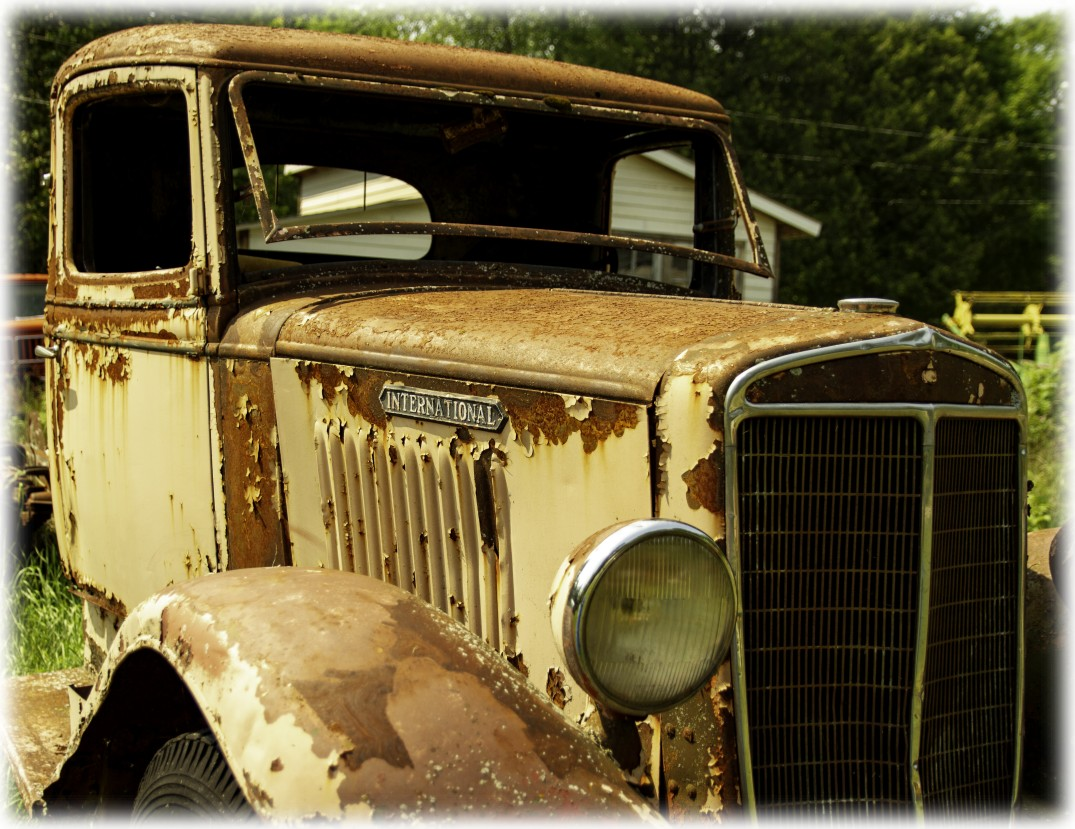
\includegraphics[width=4.0in]{figures/truck}
		\label{fig:title_figure}
	\end{figure} 
	
	\vspace{2cm}
	
	\textbf{Austin R.J. Downey}\\ Department of Mechanical Engineering \\ Department of Civil and Environmental Engineering \\ University of South Carolina, Columbia SC, USA 
	








	\vspace*{\fill}
	
	\today


\end{center}

\pagebreak

\pagebreak
\setcounter{page}{1}
\pagenumbering{roman}
\tableofcontents

\pagebreak

\setcounter{secnumdepth}{0} % Set the section depth to 0 so this is an un-umbered section in the table of contents.
\setcounter{page}{1}
\pagenumbering{arabic} 

\section{Preface}
\vspace{-1ex}
This text is a practical, example-driven guide to introduce classical machine learning techniques using the {\tt{scikit-learn}} library designed for engineers with limited to no programming experience. This preface collects the essential housekeeping information for using this text.



\vspace{-0.5ex}
\subsection{Accompanying Video Lectures}
\vspace{-1ex}
Videos of lectures associated with this text are available as a playlist 
\href{https://www.youtube.com/playlist?list=PL-2wJog-EC5-yp3CSFpj2vEcj3Pp6UcoC}{here}.

\begin{figure}[H]
	\centering
	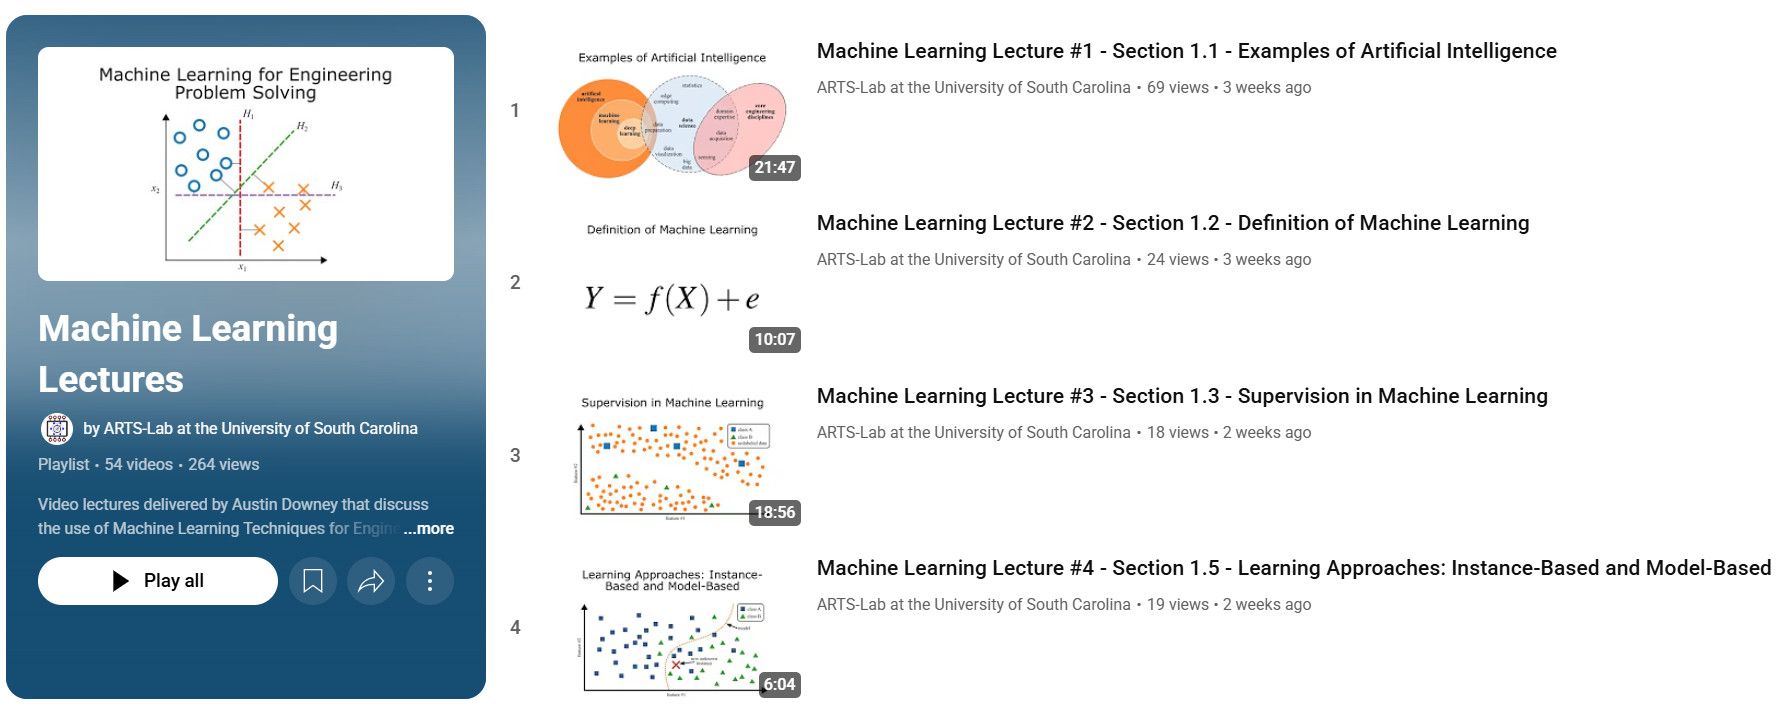
\includegraphics[width=6.0in]{figures/video_playlist}
	\vspace{-0.5ex}
	\caption{Playlist of videos associated with this text.}
	\label{fig:video_playlist}
	\vspace{-1.5ex}
\end{figure} 

\vspace{-0.5ex}
\subsection{Programming in Python}
\vspace{-1ex}
This text uses Python programmed though the Spyder IDE managed through the Anaconda platform for the examples, leveraging the {\tt{scikit-learn}} library to explain the topics discussed. To assist readers of the text, a six part video series that walks the practitioner though this combination of IDE and distribution manager is provided as a playlist  \href{https://www.youtube.com/playlist?list=PL-2wJog-EC5-wQQUdpc8MjztKZ1kE2ATS}{here}.

\begin{figure}[H]
	\centering
	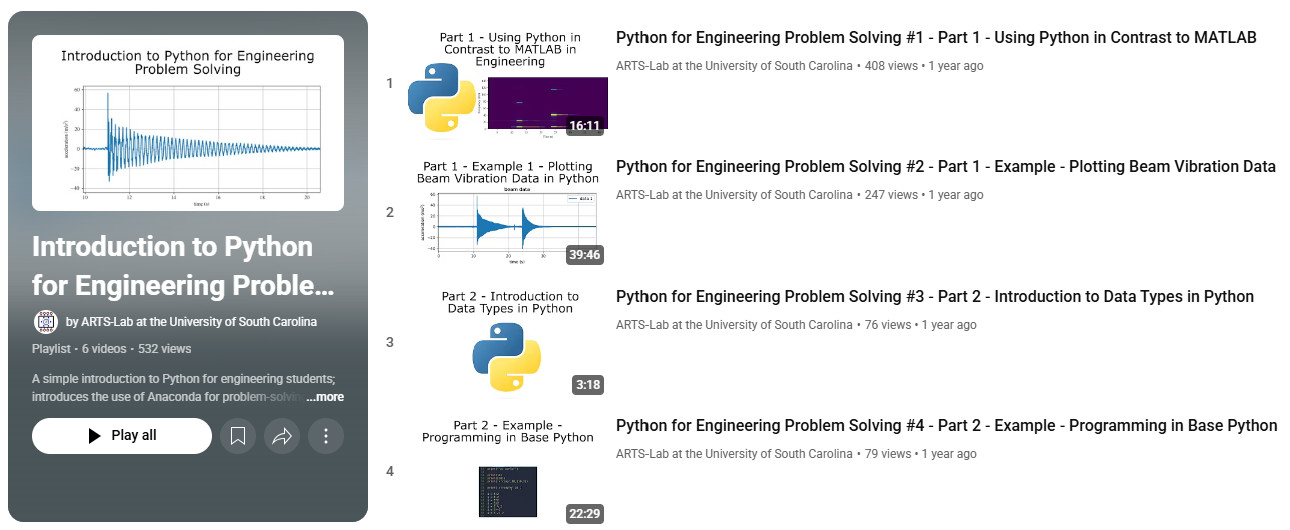
\includegraphics[width=6.0in]{figures/python_playlist}
	\vspace{-0.5ex}
	\caption{Playlist of videos for leaning how to program in Python using Spyder and Anaconda.}
	\label{fig:python_playlist}
	\vspace{-1.5ex}
\end{figure} 


\pagebreak
\clearpage                 % start the special page
\thispagestyle{noRhead}    % suppress only the right header on *this* page

\vspace{-0.5ex}
\subsection{Cover Art}
\vspace{-1ex}
The cover image, is a mid-1930s International Harvester C-series truck. Built between 1934 and 1936 at the company's Springfield Works in Springfield, Ohio. Roughly 80,000 C-series trucks where made during this short time. The C-series was International's first line to feature an all-steel cab and a host of mechanical upgrades over the prior W-series. This truck was photographed by Ethan McNeese on Washington Island in Door County, Wisconsin in 2021.

The truck on the cover underscores the simple idea that a machine's purpose is to turn raw input into useful work. The same principle drives machine learning, where digital ``machines'' transform data into insight and data-informed actions.



\vspace{-0.5ex}
\subsection{License}
\vspace{-1ex}
This work is licensed under a Creative Commons Attribution-ShareAlike 4.0 International License [cc-by-sa 4.0]. More information on the Attribution-ShareAlike 4.0 International (CC BY-SA 4.0) license can be found 
\href{https://creativecommons.org/licenses/by-sa/4.0/}{here}.
Unless otherwise denoted, all text, figures, diagrams, and photos used in this work are the sole property of the authors and are released under CC BY-SA 4.0 both in part and in whole. Reworks and redistributions of this work that fall within the CC BY-SA 4.0 licenses are encouraged.

\vspace{-0.5ex}
\subsection{Source Code}
\vspace{-1ex}
The source code for this text is available 
\href{https://github.com/austindowney/Machine-Learning-for-Engineering-Problem-Solving}{here}.




\subsection{Questions and Contact Information}
\vspace{-1ex}
For questions, corrections, or requests, contact Austin Downey at austindowney@sc.edu.


\clearpage                 	% start the special page
\setcounter{secnumdepth}{3} % reset the section depth so the following sections have numbers. The 3 means it has section, subsection, and subsubsection
\pagebreak

%%%%%%%%%%%%%		Notes on compiling Document		%%%%%%%%%%%%%
% Notes on compiling Document
%
% 1. Each chapter can be compiled on there own.
% 2. I set the document up with a common figures folder to allow for the reuse of figures and generally to keep the document clean. 
% 3. When compiling the main document, you must include the \graphicspath{{xx}} for the first chapter, to set it in chapter 1. From here on, it will think its in the chapter one folder but the <../figures> in each folder will work with this. 
% 4. I (Austin Downey) have gotten this to compile on Windows with MikTeX and Linux with TeXLive. Your results may vary. For Linux, I:
% 	i.	added the extra {} in \graphicspath
% 	ii.	removed the .tex extension from the file names except for chapter 1. 
% 5. The common bibliography is an issue that has yet to be sorted out.
%%%%%%%%%%%%%%%%%%%%%%%%%%%%%%%%%%%%%%%%%%%%%%%%%%%%%%%%%%%%%%%%%%

% Chapter 1 Basic Concepts
\graphicspath{{Chapter_1_Basic_Concepts/}}
\documentclass[12pt,letter]{article}
\usepackage{../downey_format}


\begin{document}
	
	% set the section number, along with figure and equation numbers
	\setcounter{section}{0}	
	\setcounter{figure}{\thesection}   
	\renewcommand\thefigure{\thesection.\arabic{figure}}
	\setcounter{equation}{\thesection}   
	\renewcommand\theequation{\thesection.\arabic{equation}}


\section{Basic Concepts in Machine Learning}

\begin{figure}[bp!]
    \centering
    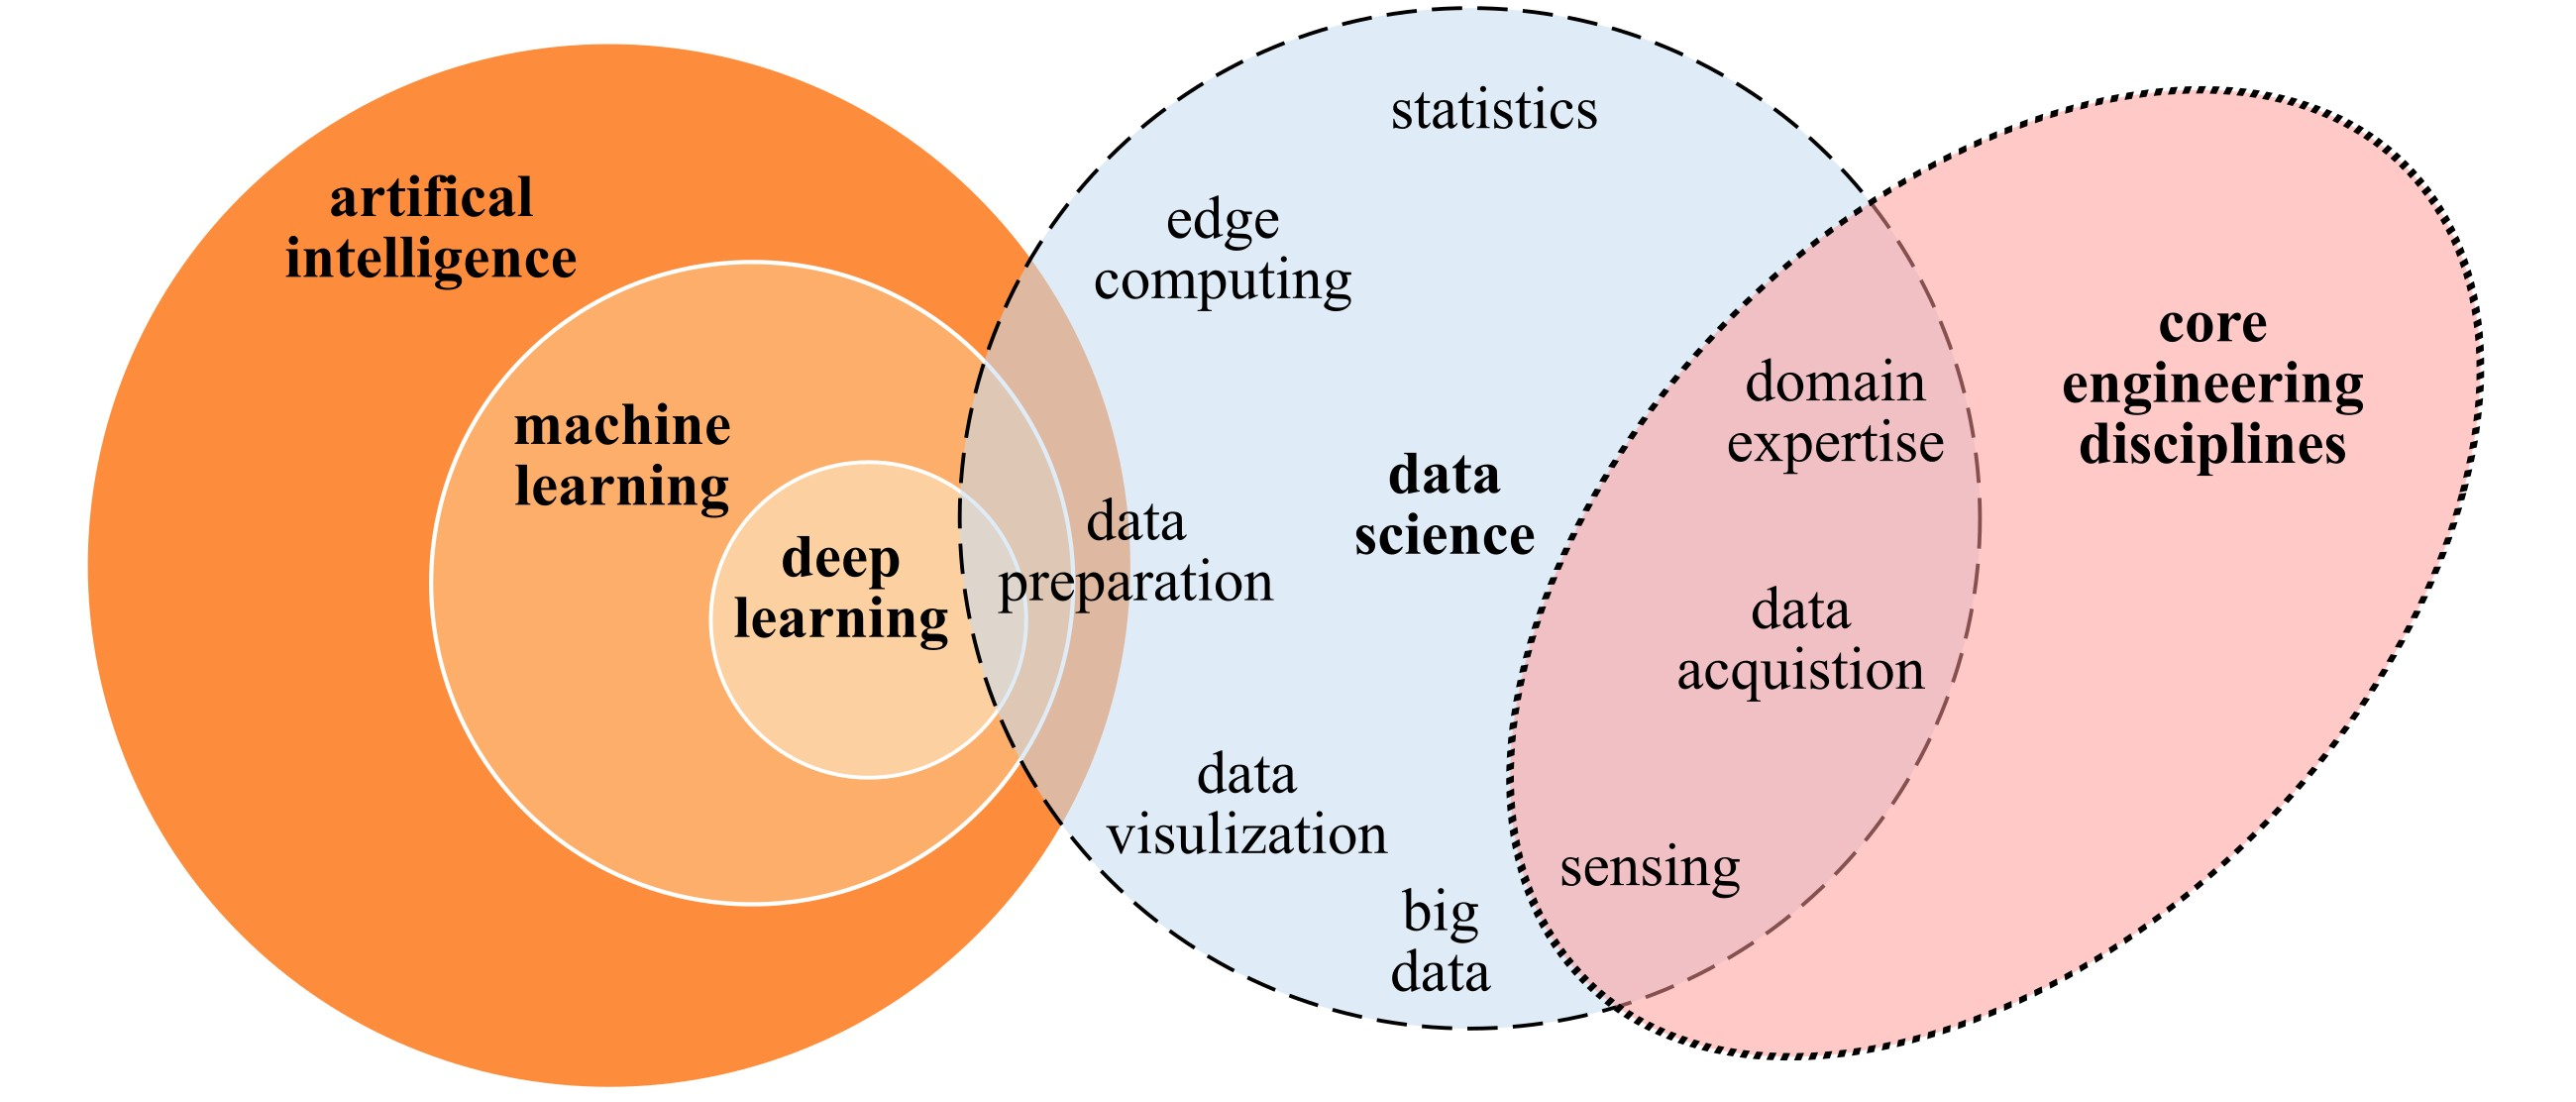
\includegraphics[width=\linewidth]{../figures/AI-vs-ML-vs-Deep-Learning}
    \caption{Overlap between the fields of Artificial Intelligence (AI), Data science (DS), and the core engineering disciplines of Civil, Mechanical, Electrical, and Chemical Engineering.}
    \label{fig:AI-vs-ML-vs-Deep-Learning}
\end{figure}

Machine Learning (ML) is a method of data analysis that automates analytical model building. ML is closely coupled to data science, as shown in figure~\ref{fig:AI-vs-ML-vs-Deep-Learning}, which is a multidisciplinary field that utilizes scientific methods, processes, algorithms, and systems to extract knowledge and insights from structured and unstructured data. It is based on the idea that systems can learn from data, identify patterns, and make decisions with minimal human intervention. This section introduces some foundational concepts in machine learning and its applications.

\begin{itemize}
    \item \textbf{ML is not creating robots}: A common misconception is that machine learning is about building robots. In reality, ML focuses on developing algorithms that can learn from and make predictions or decisions based on data.
    \item \textbf{The SPAM filter is one of the initial ML uses}: One of the earliest and most common applications of ML is the spam filter, which classifies emails as spam or not spam. This has been followed by numerous other applications such as:
    \begin{itemize}
        \item \textbf{Speech to text technology}: Converting spoken language into written text, which is used in virtual assistants and transcription services.
        \item \textbf{Medical diagnostics}: Assisting doctors by predicting diseases from medical images and patient data.
    \end{itemize}
    \item \textbf{ML has lots of fundamental concepts (jargon)}: To effectively understand and apply machine learning, it's essential to grasp several key concepts and terminologies, including:
    \begin{itemize}
        \item \textbf{Supervised vs unsupervised learning}: Supervised learning involves training a model on labeled data, while unsupervised learning deals with data that has no labels and tries to find hidden patterns.
        \item \textbf{Online versus batch learning}: Online learning algorithms update the model incrementally as new data arrives, whereas batch learning algorithms train the model using the entire dataset at once.
        \item \textbf{Instance-based vs model-based learning}: Instance-based learning algorithms, such as k-nearest neighbors, use specific instances to make predictions, whereas model-based algorithms, like linear regression, build a model from the training data and use it to make predictions.
    \end{itemize}
\end{itemize}


\begin{figure}[tp!]
    \centering
    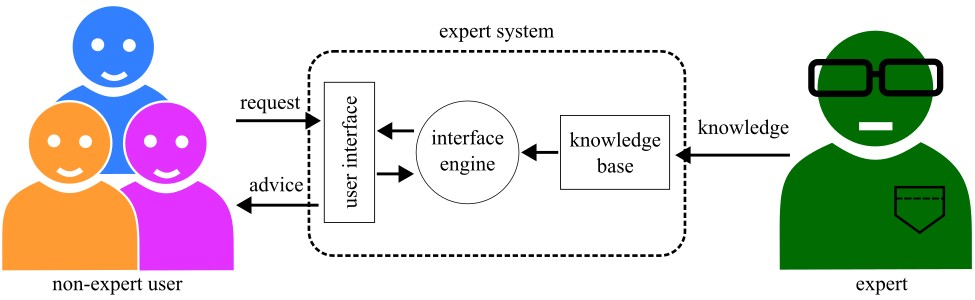
\includegraphics[width=6in]{../figures/expert_system}
    \caption{Diagram of an ``expert system'' in AI, which is a computer program that simulates the decision-making ability of a human expert by using a knowledge base and inference rules.}
    \label{fig:expert_system}
\end{figure}


\subsection{Examples of Artificial Intelligence}

The field of Artificial Intelligence (AI) encompasses a diverse array of technologies and methodologies aimed at enabling machines to perform tasks that typically require human intelligence. This section explores various examples of AI, Machine Learning, and Deep Learning technologies, highlighting their distinct characteristics and applications.

\subsubsection{Examples of Artificial Intelligence}

Artificial Intelligence (AI) encompasses a wide range of technologies aimed at making machines simulate human intelligence. Some examples include:

\begin{itemize}
    \item \textbf{Expert systems}: Computer programs that simulate the decision-making ability of a human expert by using a knowledge base and inference rules, as diagrammed in figure~\ref{fig:expert_system}.
    \item \textbf{Chatbots}: Programs designed to simulate conversation with human users, especially over the internet.
\end{itemize}



\pagebreak

\subsubsection{Examples of Machine Learning}

Machine Learning, as a subset of AI, involves algorithms that improve automatically through experience. Some common examples include:

\begin{itemize}
    \item \textbf{Linear regression}: A statistical method for modeling the relationship between a dependent variable and one or more independent variables.
    \item \textbf{Classification}: Techniques such as decision trees and support vector machines (SVMs) that categorize data into predefined classes.
    \item \textbf{Simple image/speech recognition}: Algorithms that identify objects in images or convert spoken language into text, fundamental in applications like facial recognition and virtual assistants. An example is the Symbolics Lisp Machine shown in figure~\ref{fig:Symbolics3640_Modified}.
\end{itemize}

\begin{figure}[t]
    \centering
    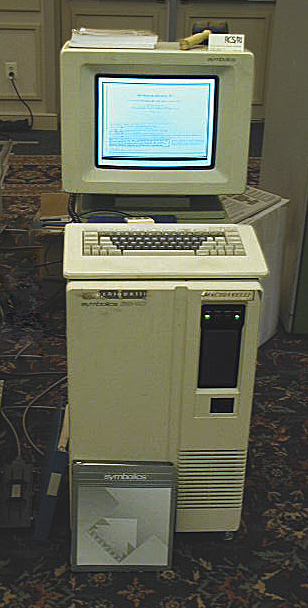
\includegraphics[width=2.2in]{../figures/Symbolics3640_Modified.jpg}
    \caption{A Symbolics Lisp Machine, a specialized hardware platform designed to run expert systems which are a version of AI focusing on answering questions to challenging problems.\protect\footnotemark[1]}
    \label{fig:Symbolics3640_Modified}
\end{figure}

\footnotetext[1]{Michael L. Umbricht and Carl R. Friend (Retro-Computing Society of RI), CC BY-SA 3.0 $<$https://creativecommons.org/licenses/by-sa/3.0$>$, via Wikimedia Commons}





\pagebreak
	\subsubsection{Examples of Deep Learning}

	
	Deep learning, an enhancement of machine learning, utilizes ``deep'' neural networks to construct knowledge graphs, as shown in figure~\ref{fig:simple_neural_network_vs_deep_learning}. Though conceptualized in the 1970s, it was initially unfeasible due to the problem of vanishing gradients within the networks. In 2012, Geoffrey E. Hinton's team demonstrated that a network with 60 million parameters and 650,000 neurons could effectively perform image classification across a dataset containing 1,000 categories (paper shown in figure~\ref{fig:imageNet_classificatoin_paper}). This breakthrough was facilitated by the use of GPUs and a novel regularization technique known as ``dropout.'' The team's modified model participated in the ILSVRC-2012 competition, securing a first-place top-5 test error rate of 15.3\%, a significant improvement over the 26.2\% recorded by the runner-up and a major leap when compared to the previous year as diagrammed in figure~\ref{fig:ImageNet-competition-results}.

		\begin{figure}[t]
			\centering
			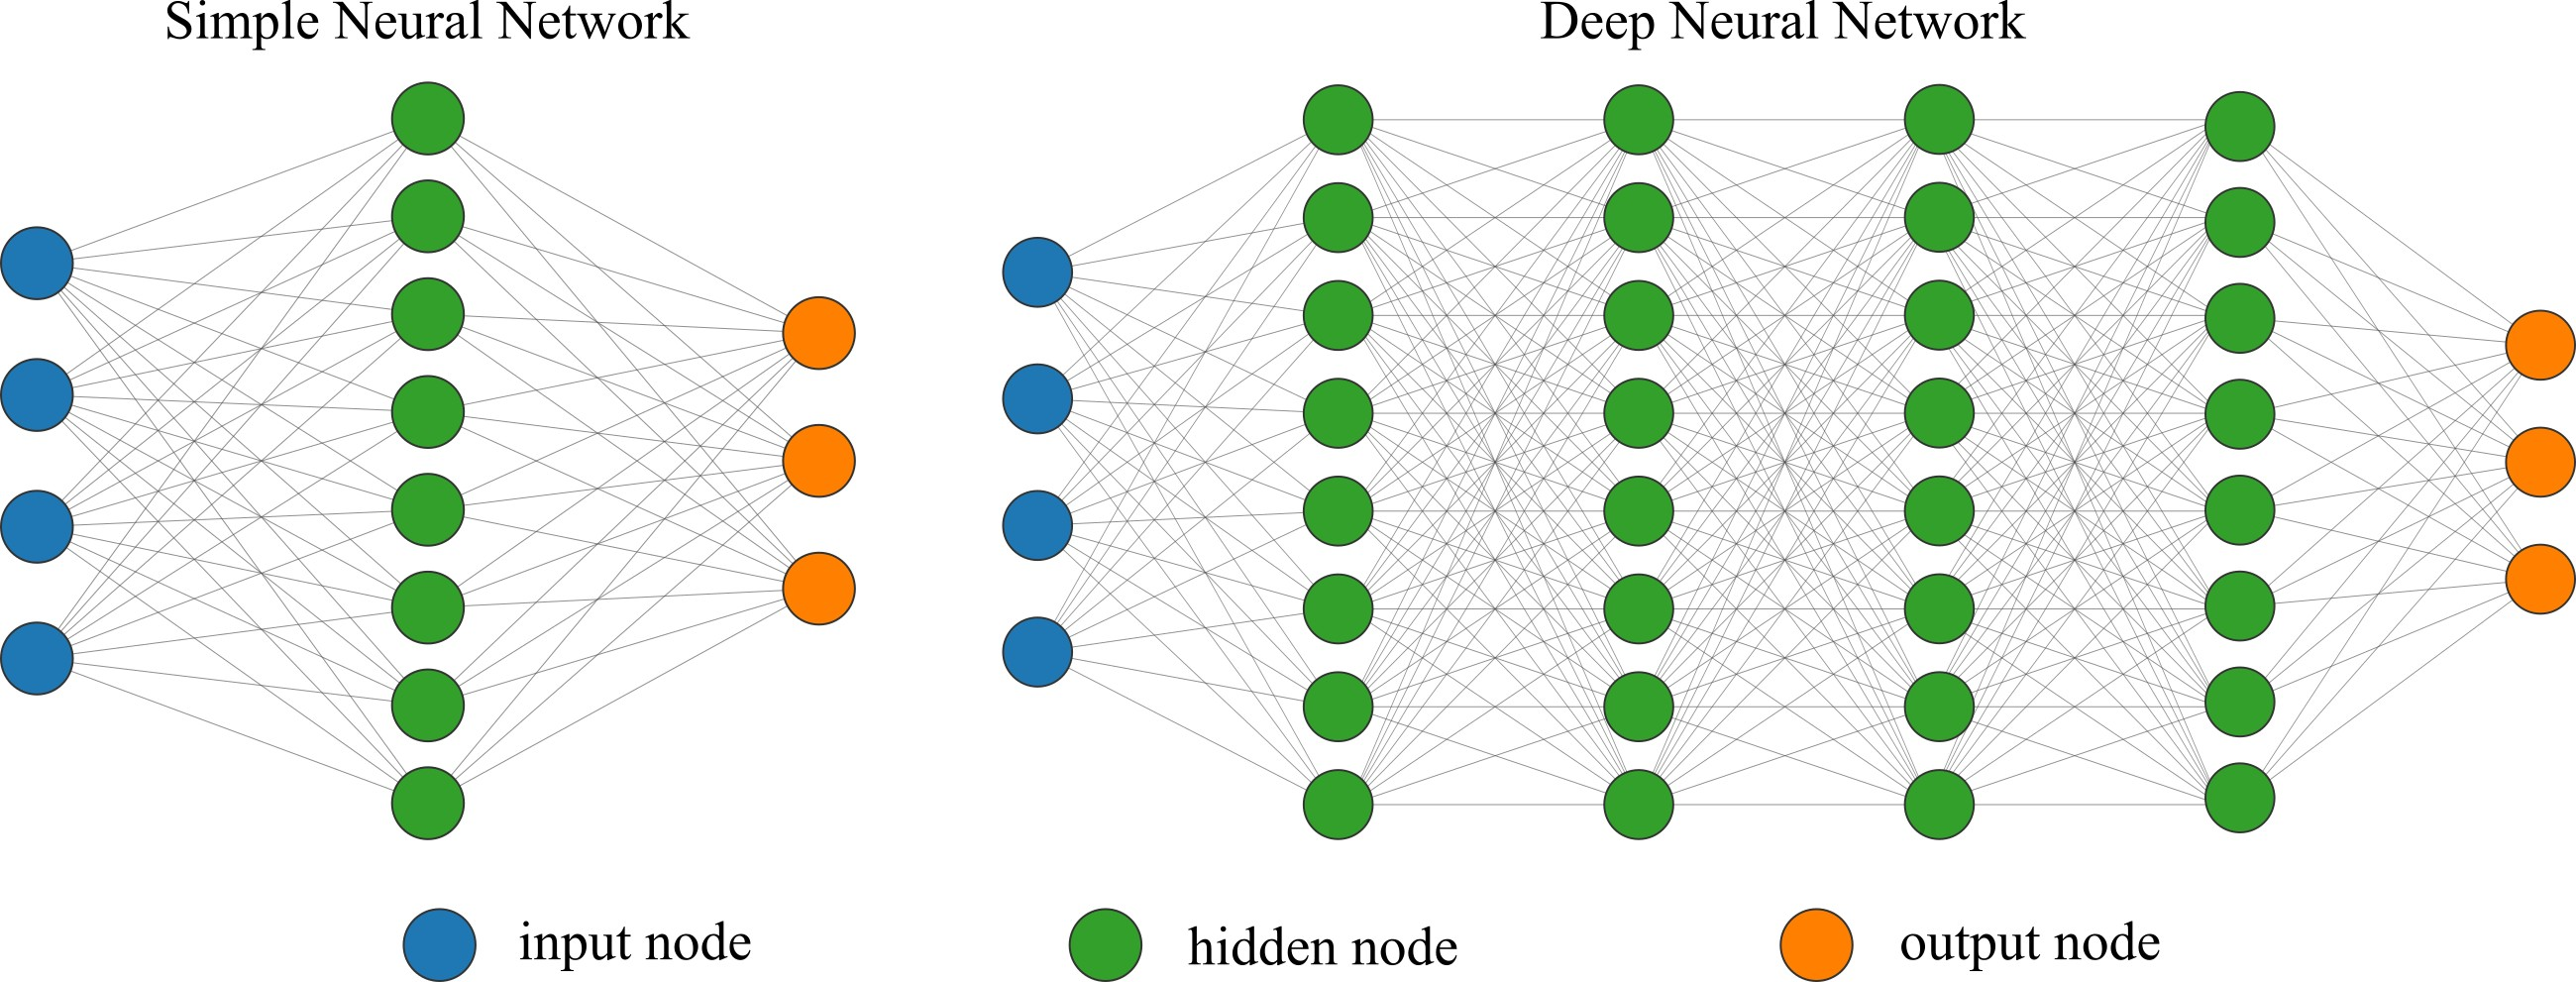
\includegraphics[width=6.5in]{../figures/simple_neural_network_vs_deep_learning.jpg}
			\caption{simple neural network vs deep learning}
			\label{fig:simple_neural_network_vs_deep_learning}
		\end{figure}

\pagebreak
	\begin{data}

		Imagenet in 2012 represented a significant step forward in machine learning by introducing the first practical example of deep learning, famously known as AlexNet (Figure~\ref{fig:imageNet_classificatoin_paper}) This model, developed by Geoffrey Hinton and his team, utilized deep convolutional neural networks to dramatically improve the accuracy of image classification, which was a longstanding challenge in the field.


		\begin{figure}[H]
			\centering
			\vspace{-2ex}
			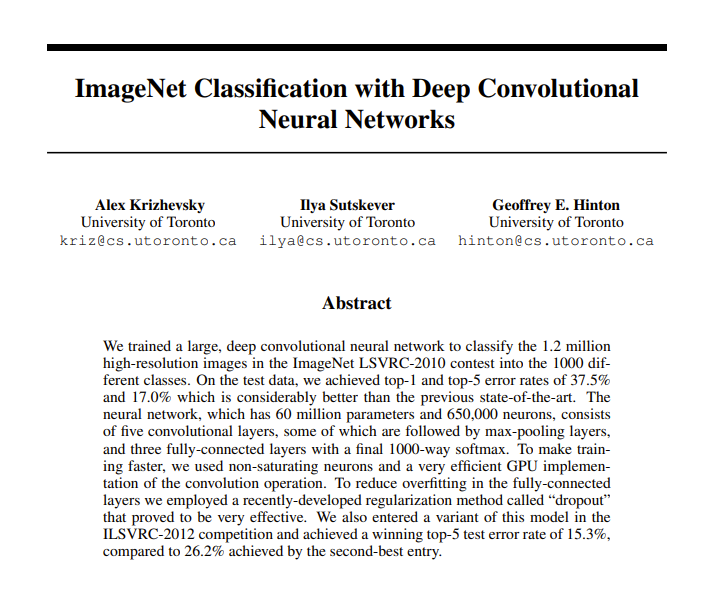
\includegraphics[width=5.0in]{../figures/imageNet_classificatoin_paper}
			\vspace{-4ex}
			\caption{Geoffrey's 2012 paper ``ImageNet Classification with Deep Convolutional Neural Networks''.\protect\footnotemark[1]}
			\label{fig:imageNet_classificatoin_paper}
		\end{figure}
		\footnotetext[1]{Copyright held by Authors and Neural Information Processing Systems Foundation, Inc., used under fair use. $<$https://proceedings.neurips.cc/paper/2012/file/c399862d3b9d6b76c8436e924a68c45b-Paper.pdf$>$}

		The results of AlexNet were rather monumental, reducing the top-5 test error rate to 15.3\% compared to 26.2\% by the next best entry, as shown in Figure~\ref{fig:ImageNet-competition-results}.  This was clear evidence of deep learning's superior capability over traditional machine learning methods, effectively revolutionizing the approach towards machine learning in the broader scientific community.

		\begin{figure}[H]
			\centering
			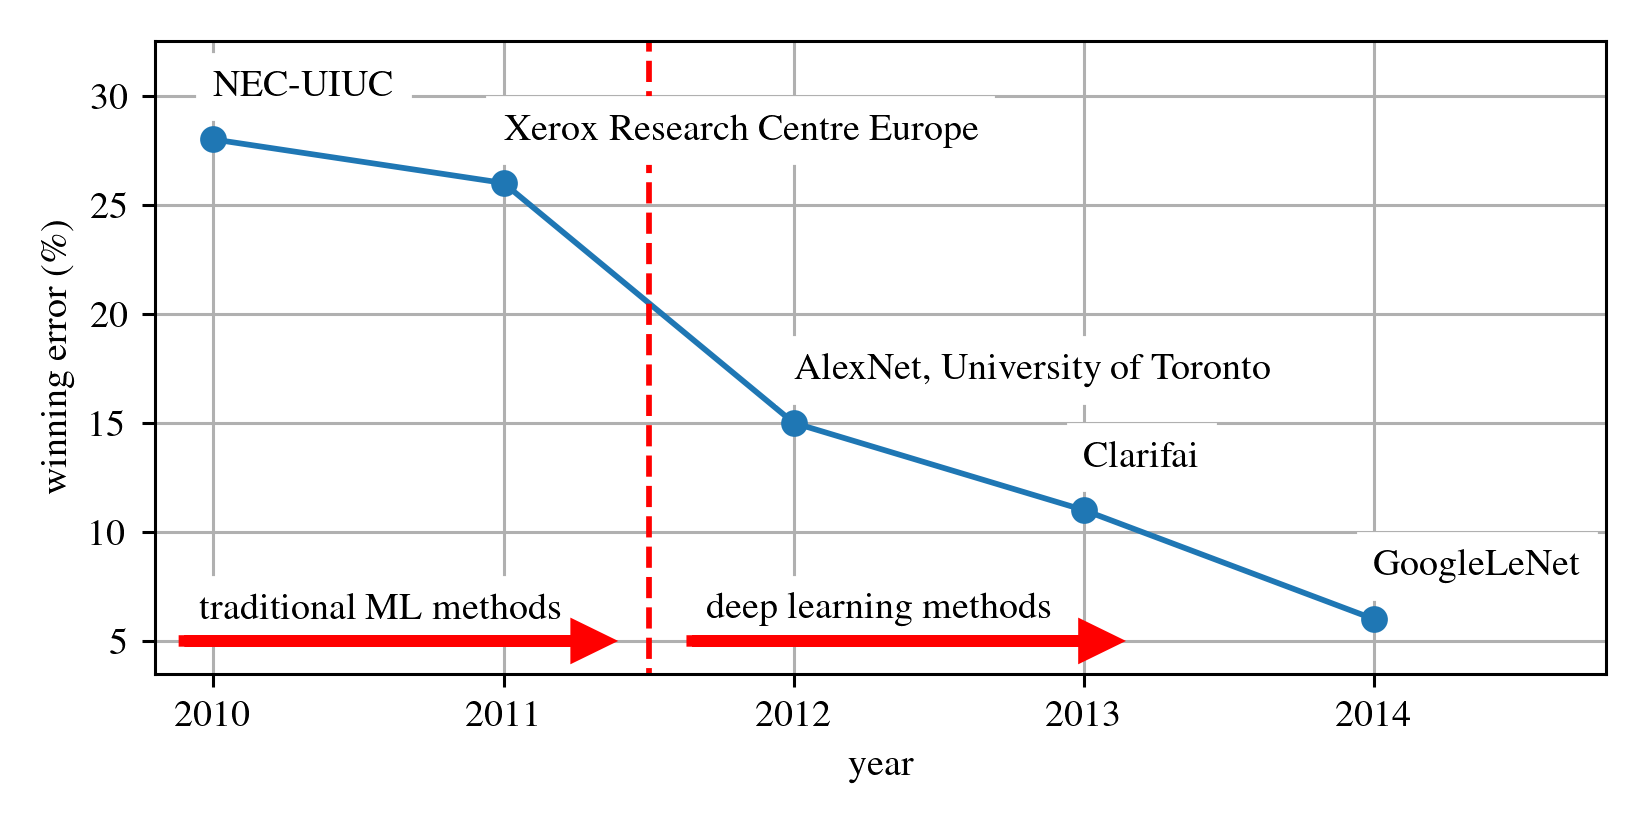
\includegraphics[width=4.95in]{../figures/ImageNet-competition-results}
			\caption{ImageNet Competition Results showing the impact of deep learning methods on image classification.}
			\label{fig:ImageNet-competition-results}
		\end{figure}

		The implications of this leap forward led to broad applications of deep learning that permeate numerous aspects of technology and science today. The impact of AlexNet and subsequent deep learning developments culminated in the awarding of the 2024 Nobel Prize in Physics to Geoffrey Hinton, recognizing his contributions to the field of artificial neural networks. Figure~\ref{fig:Nobel} shows the 2024 Nobel Award Ceremony in Stockholm Sweden with John Hopfield and Geoffrey Hinton receiving their awards from the King of Sweden. 

		\begin{figure}[H]
			\centering
			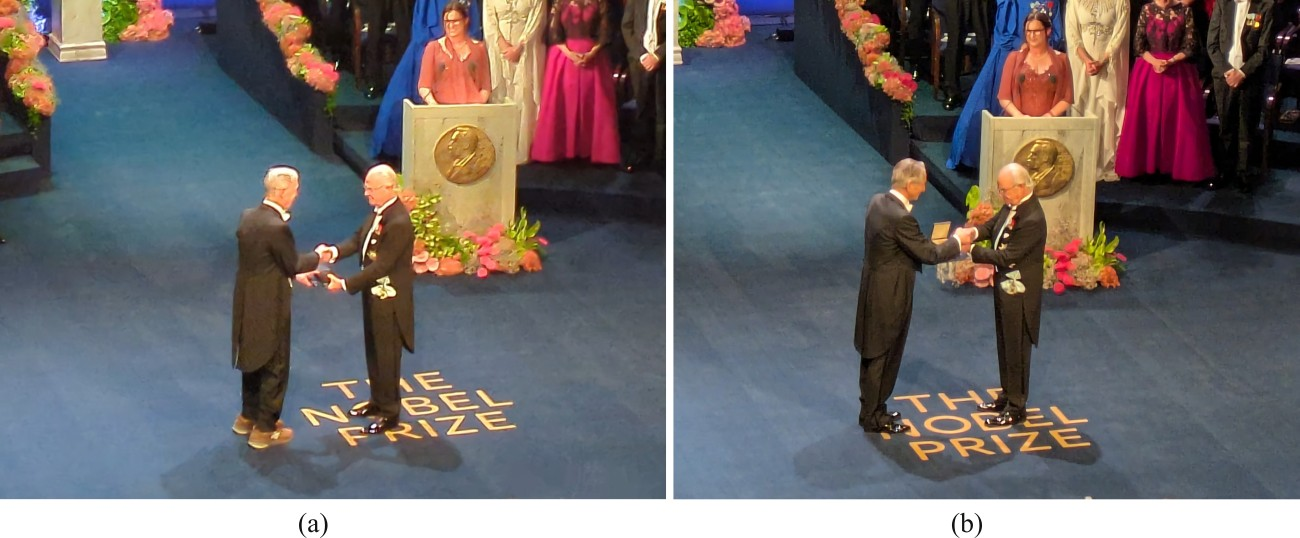
\includegraphics[width=4.95in]{../figures/Nobel}
			\caption{The 2024 Nobel Prize in Physics for ``for foundational discoveries and inventions that enable machine learning with artificial neural networks'' was awarded to: (a) John Hopfield and (b) Geoffrey  Hinton. \protect\footnotemark[1]}
			\label{fig:Nobel}
		\end{figure}
		\footnotetext[1]{The author of this text was lucky enough to attend the 2024 Nobel Prize Ceremony in Stockholm and took these pictures.}

	\end{data}


	\subsection{Definition of Machine Learning}

	The definitions and conventions that follow provide a common language and point of reference for all subsequent material:

		\begin{itemize}
			\item	Machine learning is the discipline of creating computer programs that improve automatically by analyzing data. Here a broader and a more engineering-focused definition of Machine learning is provided5:
			\begin{itemize}
				\item {[Machine Learning is the]} field of study that gives computers the ability to learn without being explicitly programmed. Arthur Samuel, 1959.
				\item A computer program is said to learn from experience E with respect to some task T and some performance measure P, if its performance on T, as measured by P, improves with experience E. Tom Mitchell, 1997.
			\end{itemize}
			\item The use of $X$ and $Y$ for variables. 
			\begin{itemize}
				\item For the $i^{\text{th}}$ sample, $x^{(i)}$ contains all its input features (excluding the target), while $y^{(i)}$ denotes the corresponding target value.
				\item General definition:	``Machine learning algorithms are described as learning a target function ($f$) that best maps input variables ($X$) to an output variable ($Y$).''
			\end{itemize}
		\end{itemize}
		
		\begin{equation}
			Y = f(X)
		\end{equation}
		
		\noindent This is described as a standard learning challenge where the goal is to predict future values $Y$ using new samples of input variables $X$. The function $f$ that relates inputs to outputs is not known. If it were, direct application would be possible, eliminating the necessity for learning it via machine learning methods. This process is more complex than it may initially seem. Furthermore, there is an error $e$ associated with this task that is independent of the input data $X$.

	
		\begin{equation}
			Y = f(X) + e
		\end{equation}
		
		\noindent This yields two primary phases in the machine-learning workflow:
		\begin{itemize}
			\item Training: Creating the model is a compute-intensive process often run in a data center
			\item Inference: Using the model can be computationally cheap and even performed ``at the edge''
		\end{itemize}

\pagebreak

			\begin{figure}[t]
				\centering
				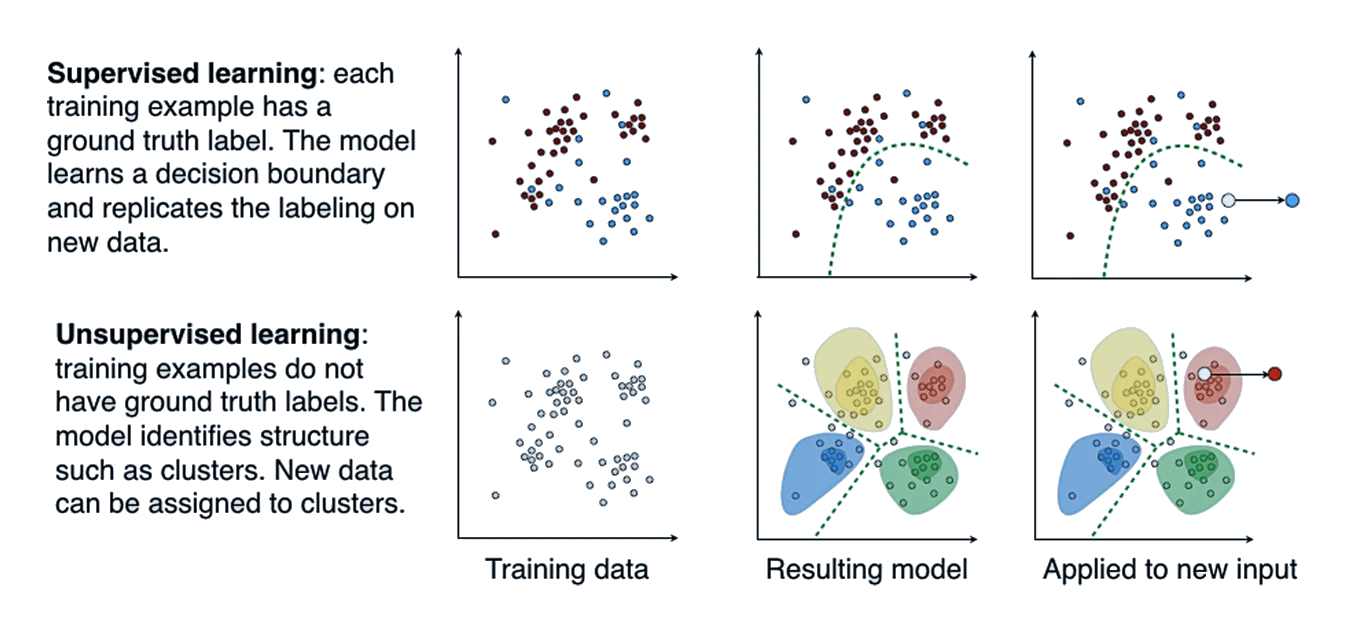
\includegraphics[width=\linewidth]{../figures/Supervised_and_unsupervised_machine_learning.png}
				\vspace{-6ex}
				\caption{Supervised vs unsupervised unsupervised machine learning methods\protect\footnotemark[1].}
				\label{fig:Supervised_and_unsupervised_machine_learning}
				\vspace{-1ex}
			\end{figure}

		\footnotetext[1]{modified from: Langs, G., R�hrich, S., Hofmanninger, J. et al., CC BY 4.0 $<$https://creativecommons.org/licenses/by/4.0$>$, via Wikimedia Commons}



	\subsection{Supervision in Machine Learning}
	\vspace{-1ex}

		The general domains of ML can be classified into supervised and unsupervised learning, as shown in figure~\ref{fig:Supervised_and_unsupervised_machine_learning}.

		
		\subsubsection{Supervised Learning}
	\vspace{-1ex}			
			In supervised learning, the data is pre-categorized with labels
			\begin{itemize}[itemsep=0.0ex,topsep=0.0ex]
				\item \textbf{Classification}, The process of categorizing a given set of data into classes
				\item \textbf{Regression}, The process of estimating the relationships between a dependent variables (i.e. output) and one or more independent variables (i.e. input).
			\end{itemize}
			In supervised learning, the training data provided to the algorithm includes the desired solutions, known as labels. A common task within this type of learning is classification. An example of classification is a spam filter, which is trained using numerous emails that are each labeled as either spam or ham. The objective for the spam filter is to learn how to accurately classify new emails based on this training. Regression is another typical task is to predict a target numeric value, such as the price of a house, given a set of features (size, proximity to railroad or highways, age of house, style, etc.) called predictors. To train a system you need to build a model and train in on many house sale examples, including both predictors (house features) and their labels (i.e., prices).
			Some of the most important supervised learning algorithms:
			\begin{itemize}[itemsep=0.0ex,topsep=0.0ex]
				\item	k-Nearest Neighbors
				\item	Linear Regression
				\item	Logistic Regression
				\item	Support Vector Machines (SVMs)
				\item	Decision Trees and Random Forests
				%\item	Neural networks (some)
			\end{itemize}
			
%			\begin{figure}[t]
%				\centering
%				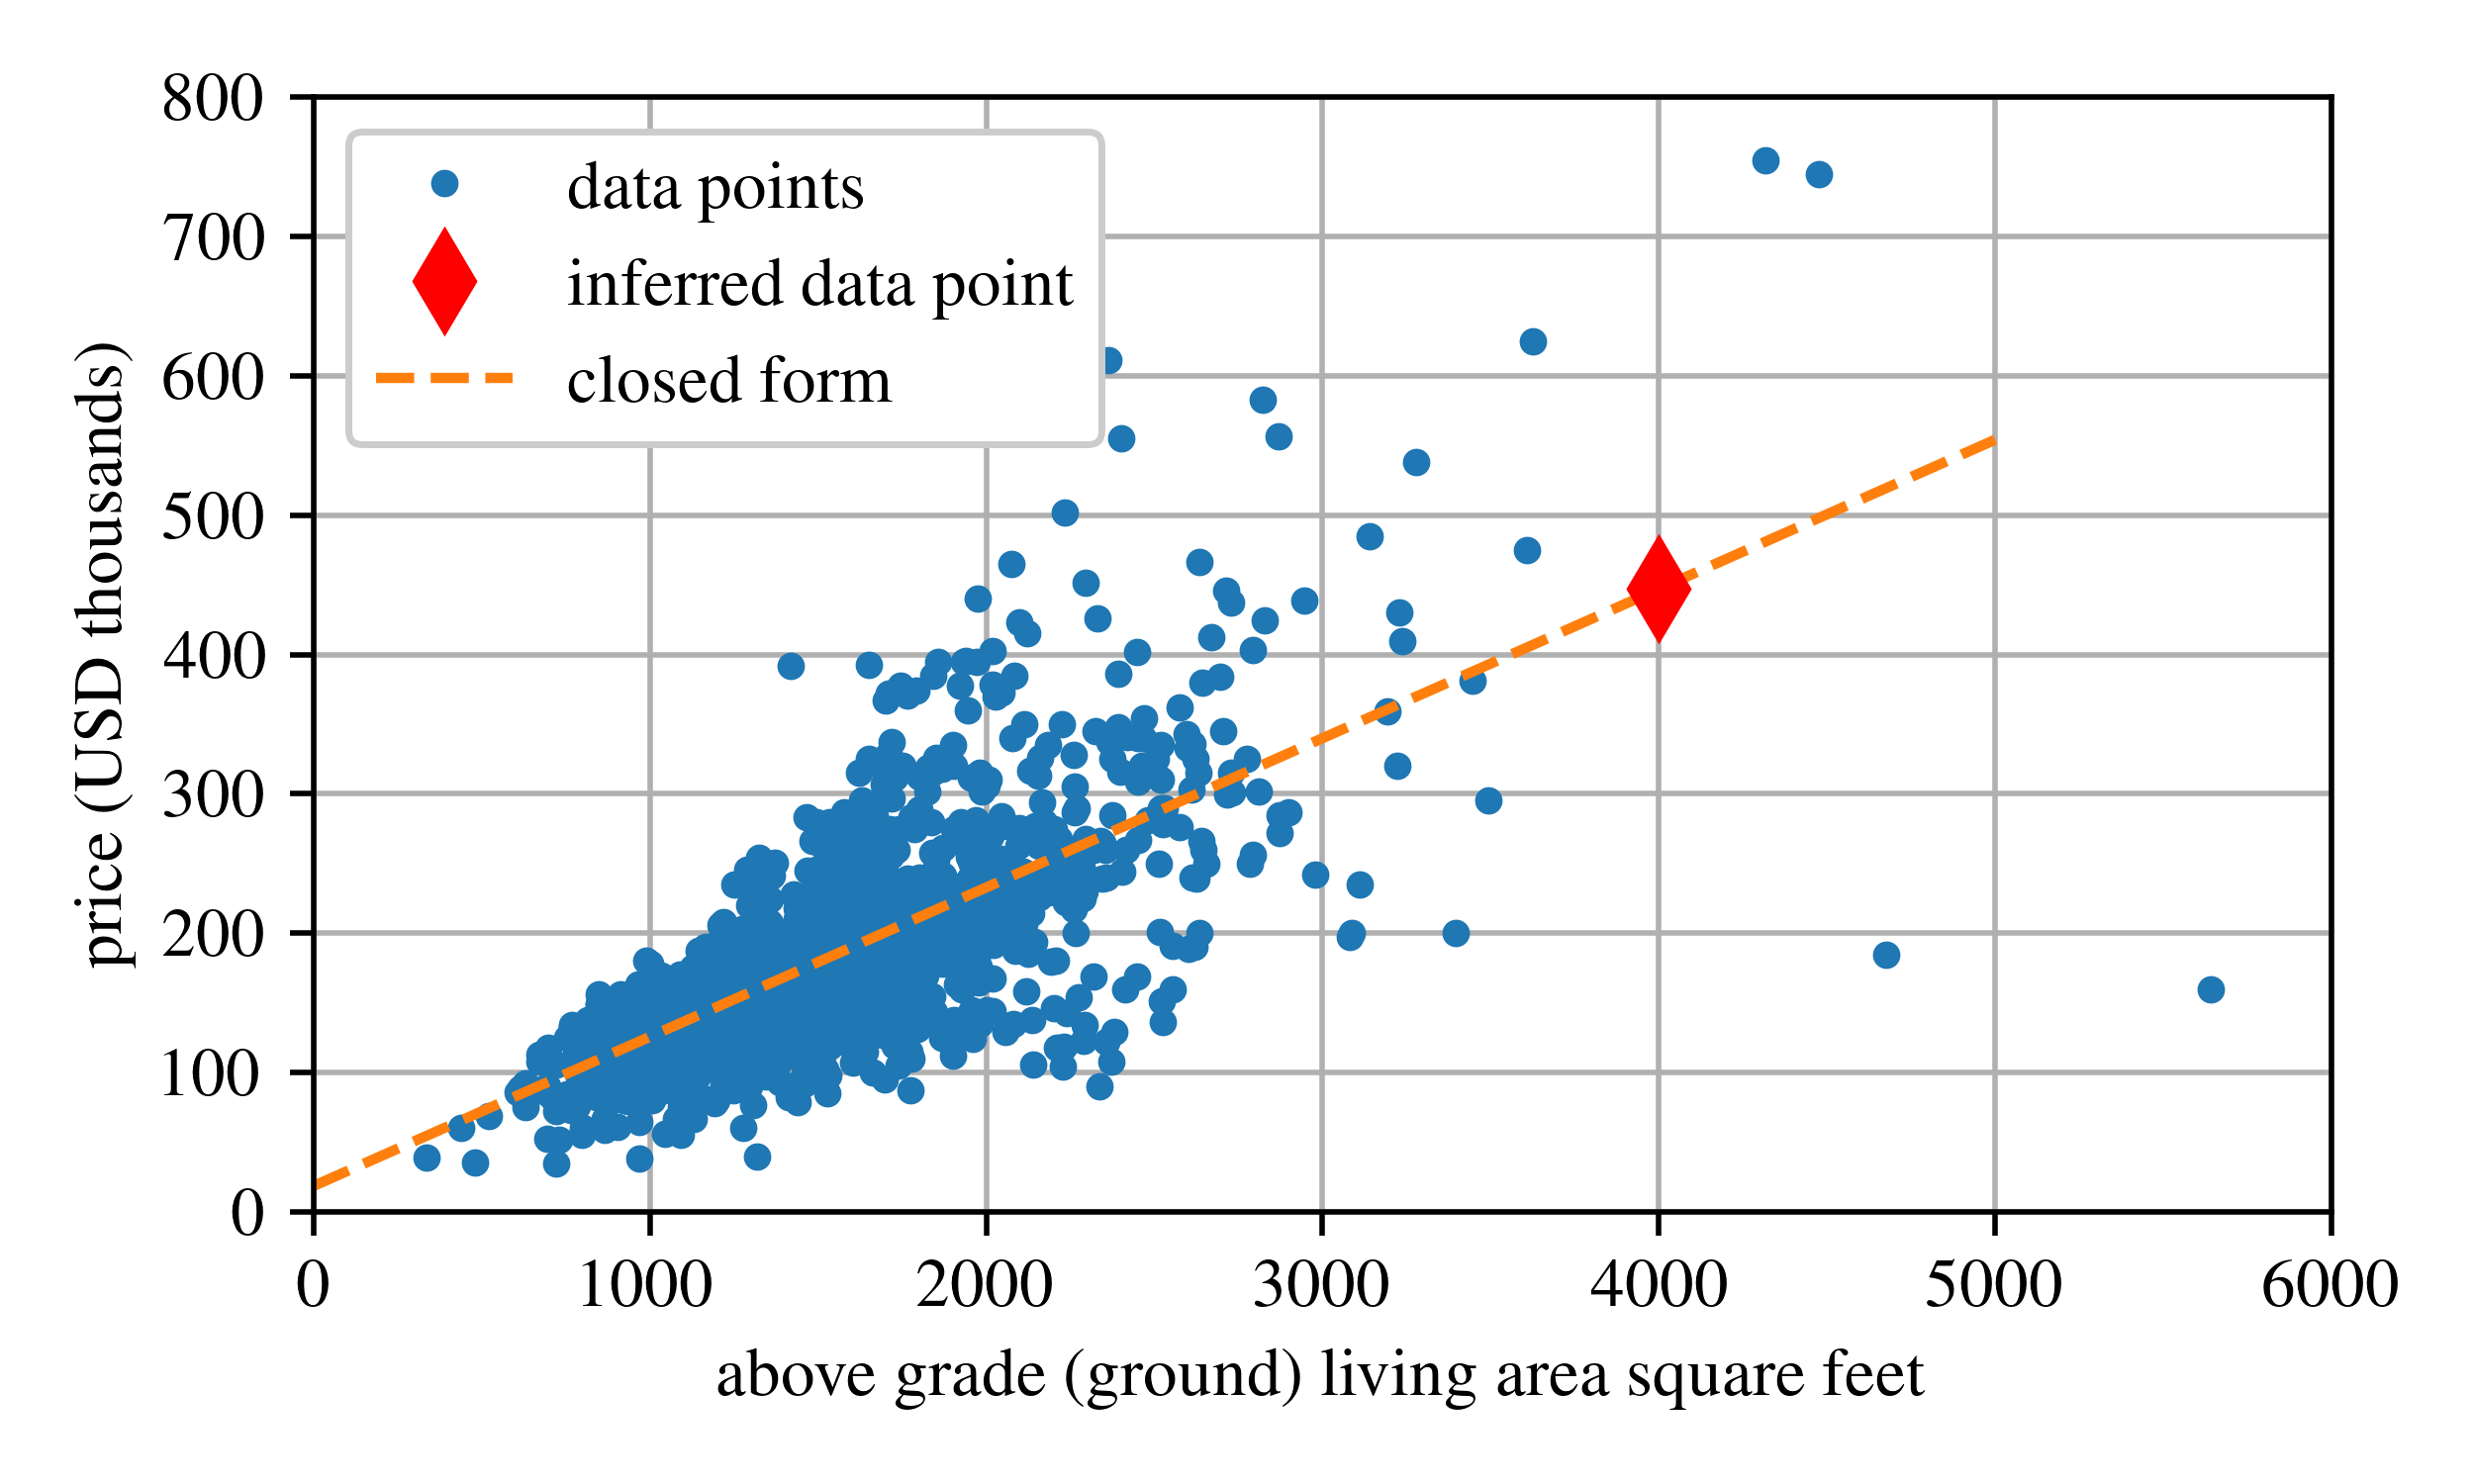
\includegraphics[]{../figures/Ames_simple_linear_regression_model_3}
%				\caption{Estimating the price of a house using the area of its living space.}
%				\label{fig:Boston_simple_linear_regression_model_3}
%			\end{figure}





			
			

			\begin{figure}[H]
				\centering
				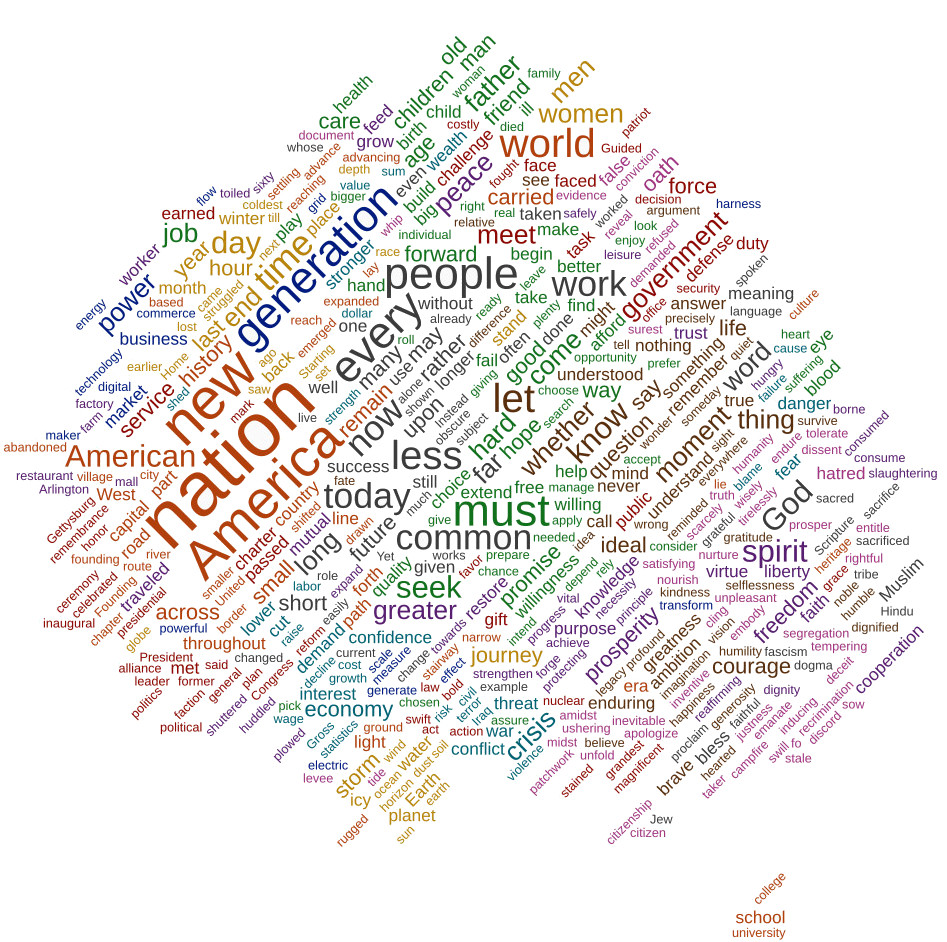
\includegraphics[width=4in]{../figures/semantic_word_cloud}
				\caption{A semantic word cloud of Barack Obama's First Inaugural Address \protect\footnotemark[1].}
				\label{fig:data_visualization}
			\end{figure}

		\footnotetext[1]{Modified from: GuoYongzhi, CC BY-SA 4.0 $<$https://creativecommons.org/licenses/by-sa/4.0$>$, via Wikimedia Commons}

			
		\subsubsection{Unsupervised Learning }

In unsupervised learning, the training data is unlabeled, and the system endeavors to learn independently without explicit guidance. For instance, consider a situation where you have extensive data on what people watch on YouTube. You might use a clustering algorithm to identify groups of similar users. However, at no point do you instruct the algorithm on which group a user belongs to; it discovers these connections autonomously. For example, it might identify that the types of videos people watch are closely linked to specific age and income metrics. Older viewers may prefer watching videos about vacations, while younger viewers might watch a lot of educational content, such as Khan Academy.

Visualization algorithms such as that in Figure~\ref{fig:data_visualization}) serve as an important instance of unsupervised learning algorithms: they take in extensive, complex, and unlabeled data and produce a 2D or 3D representation that can be conveniently visualized. These algorithms strive to maintain as much of the original data structure as possible (for example, ensuring that distinct clusters in the input space do not merge in the visual output). This helps in comprehending the organizational structure of the data and potentially uncovering hidden patterns. Other Important concepts in unsupervised learning include
\pagebreak
\begin{itemize}
	\item \textbf{Clustering}, The process of identifying and grouping similar data points in larger datasets without concern for the specific outcome
	\item \textbf{Association}, The process learning a rule-based method for discovering relations between variables data data
	\item \textbf{Dimension Reduction},  The process of reducing the number of input variables in training data.
\end{itemize}
Here are some of the most important unsupervised learning algorithms:
	\begin{itemize}
		\item	Clustering
		\item	k-Means
		\item	Hierarchical Cluster Analysis (HCA)
		\item	Expectation Maximization
	\end{itemize}



%\begin{figure}[H]
%    \centering
%    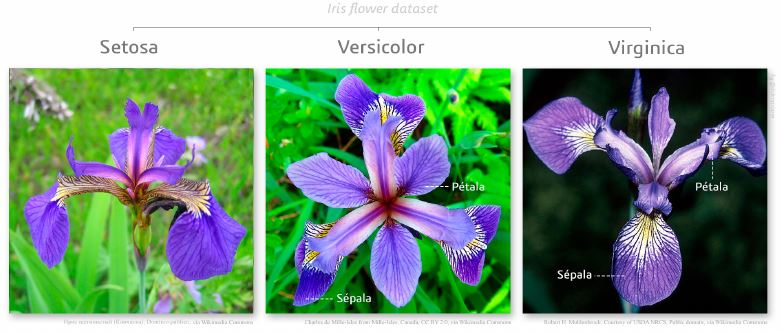
\includegraphics[width=6.5in]{../figures/iris_species}
%    \caption{Flowers representing three species of iris plants \protect\footnotemark[1]}
%    \label{fig:iris_species}
%\end{figure}
%\footnotetext[1]{Diego Mariano, CC BY-SA 4.0 $<$https://creativecommons.org/licenses/by-sa/4.0$>$, via Wikimedia Commons}


	
	

%		\begin{figure}[H]
%			\centering
%			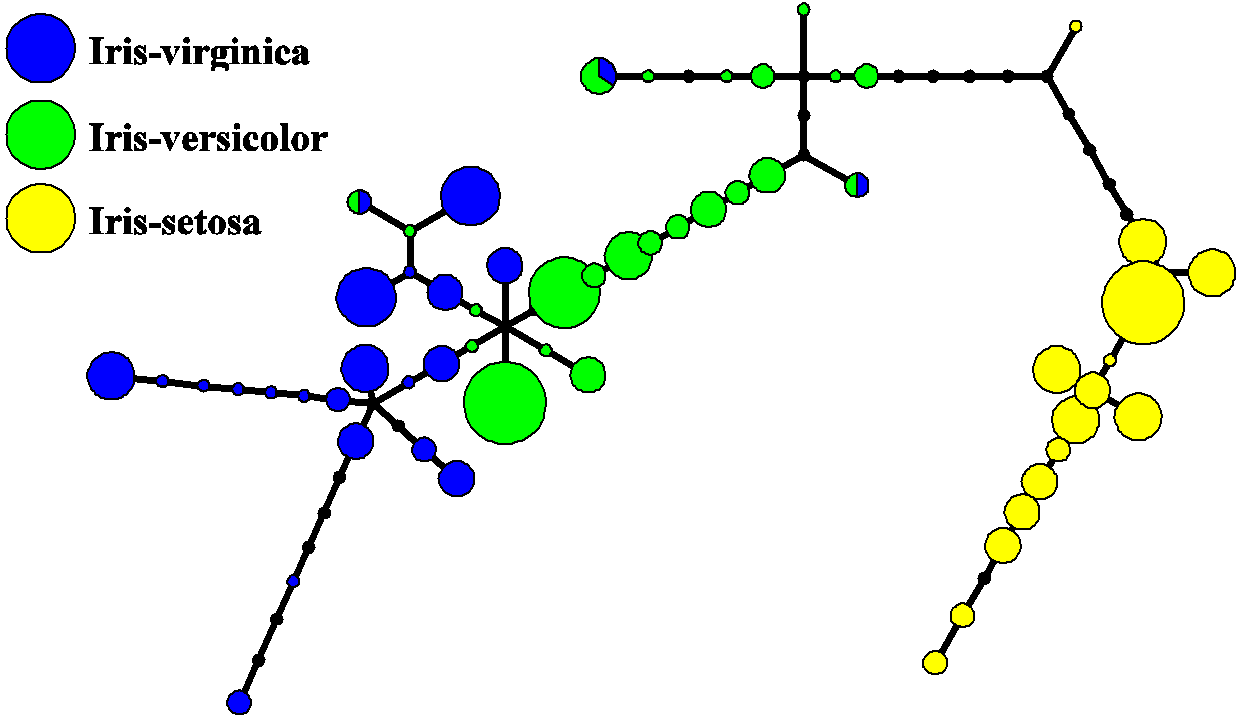
\includegraphics[width=5.5in]{../figures/Principal_tree_for_Iris_data_set.png}
%			\caption{Principal tree visualization for the Iris data set \protect\footnotemark[1]. }
%			\label{fig:Principal_tree_for_Iris_data_set}
%		\end{figure}
%		\footnotetext[1]{Agor153, CC BY-SA 3.0 $<$https://creativecommons.org/licenses/by-sa/3.0$>$, via Wikimedia Commons}
%


%			\begin{figure}[H]
%				\centering
%				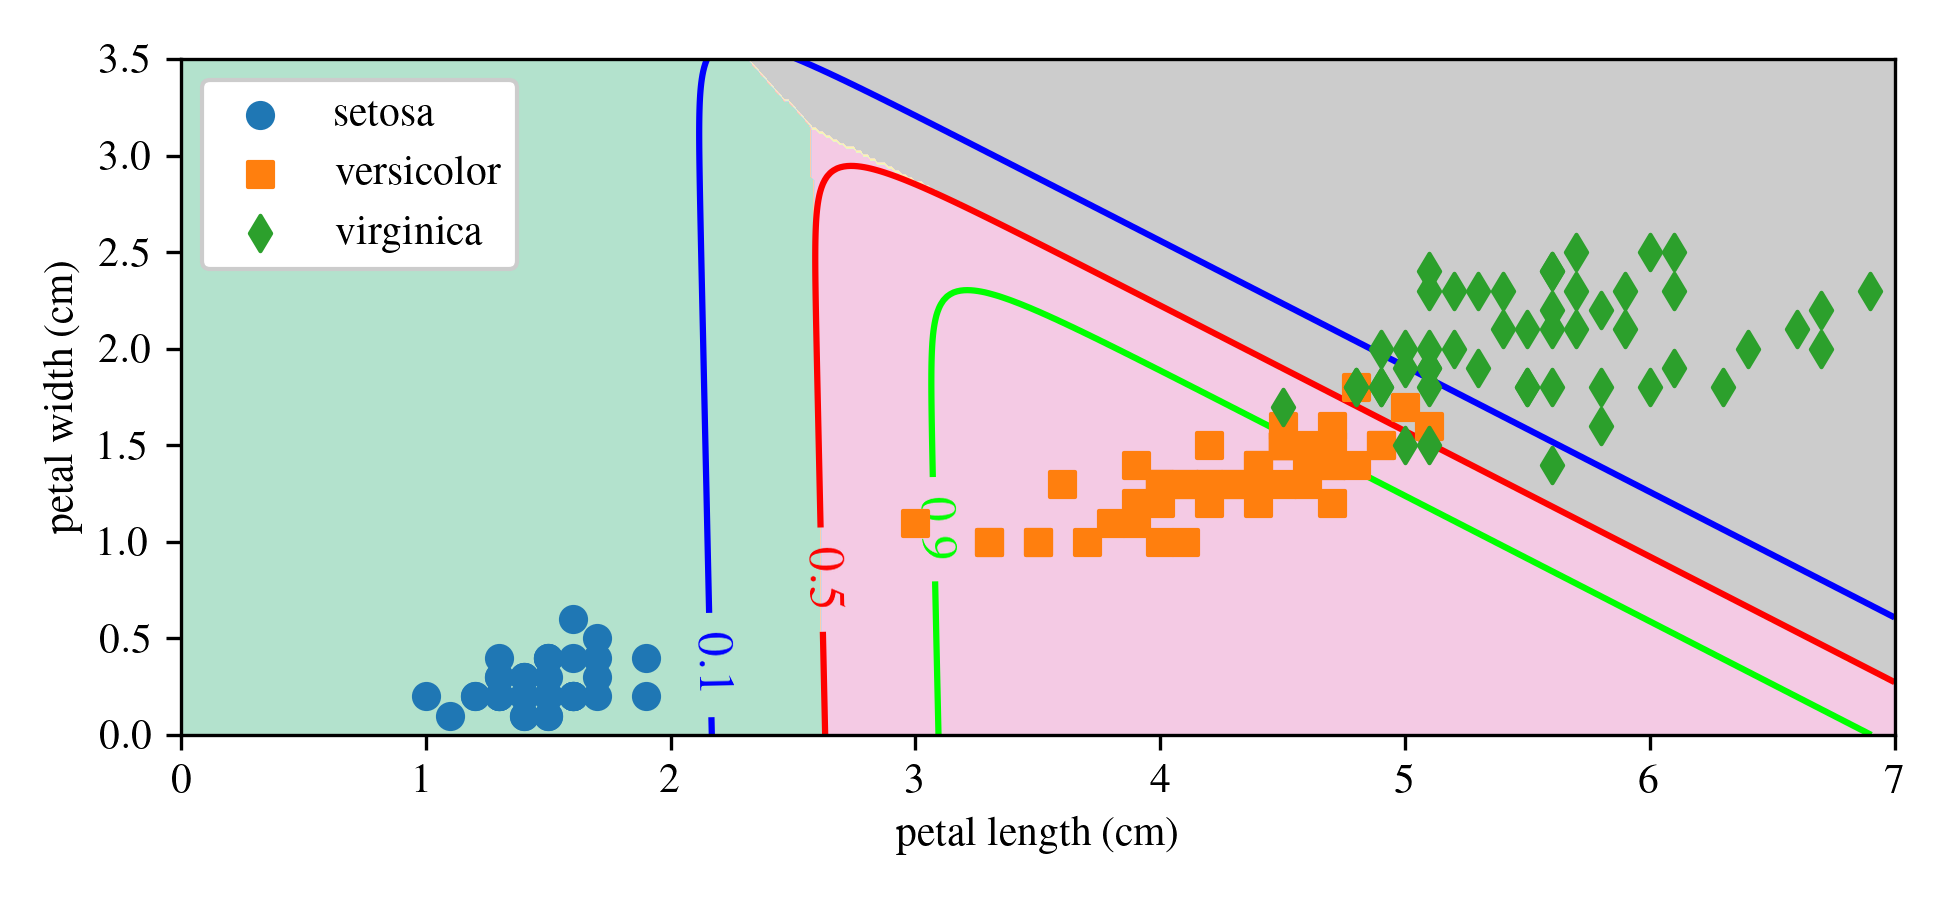
\includegraphics[width=5.5in]{../figures/Softmax_classification.png}
%				\caption{Classification of the three species for the Iris data set.}
%				\label{fig:Softmax_classification}
%			\end{figure}




%\begin{itemize}
%\item	Some important visualization items we will look at in class include. 
%				\begin{itemize}
%					\item	Principal Component Analysis (PCA)
%					\item	Kernel PCA
%					\item	Locally-Linear Embedding (LLE)
%					\item	t-distributed Stochastic Neighbor Embedding (t-SNE)
%				\end{itemize}
%\end{itemize}		

			
			\begin{figure}[H]
			\centering
				\includegraphics[width=6.5in]{../figures/Anomaly_detection}
				\caption{Anomaly Detection for a given set of data.}
				\label{fig:Anomaly_detection}
			\end{figure}
			
Another key application of unsupervised learning is anomaly detection as shown in figure~\ref{fig:Anomaly_detection}. The goal is to flag unusual credit-card transactions that may signal fraud, spot defects on a production line, or filter out outliers before passing a dataset to another learning algorithm. The model is first exposed to many examples of normal behavior so it can build a reference profile. When a new observation arrives it checks how closely the example matches that profile and labels it normal or anomalous accordingly.


		
		\subsubsection{Semisupervised Learning}
			
			Certain algorithms are designed to manage partially labeled training data, typically characterized by a substantial amount of unlabeled data with a minimal amount of labeled data  as shown in figure~\ref{fig:semisupervised_learning}.
			Many semi-supervised learning algorithms are hybrid forms, integrating features of both unsupervised and supervised learning approaches.
			
			An example is seen in image hosting services like Google Photos. Upon uploading your family images, the system automatically recognizes and groups repeated appearances of the same individuals across different photos, such as person 1 in photos A, C, and D and person 2 in photos A, B, and E. This clustering is the unsupervised component of the algorithm. The system then only needs a single label for each person to subsequently identify and tag everyone in all images, enhancing the ease of searching through photos.

			
			
			\begin{figure}[H]
				\centering
				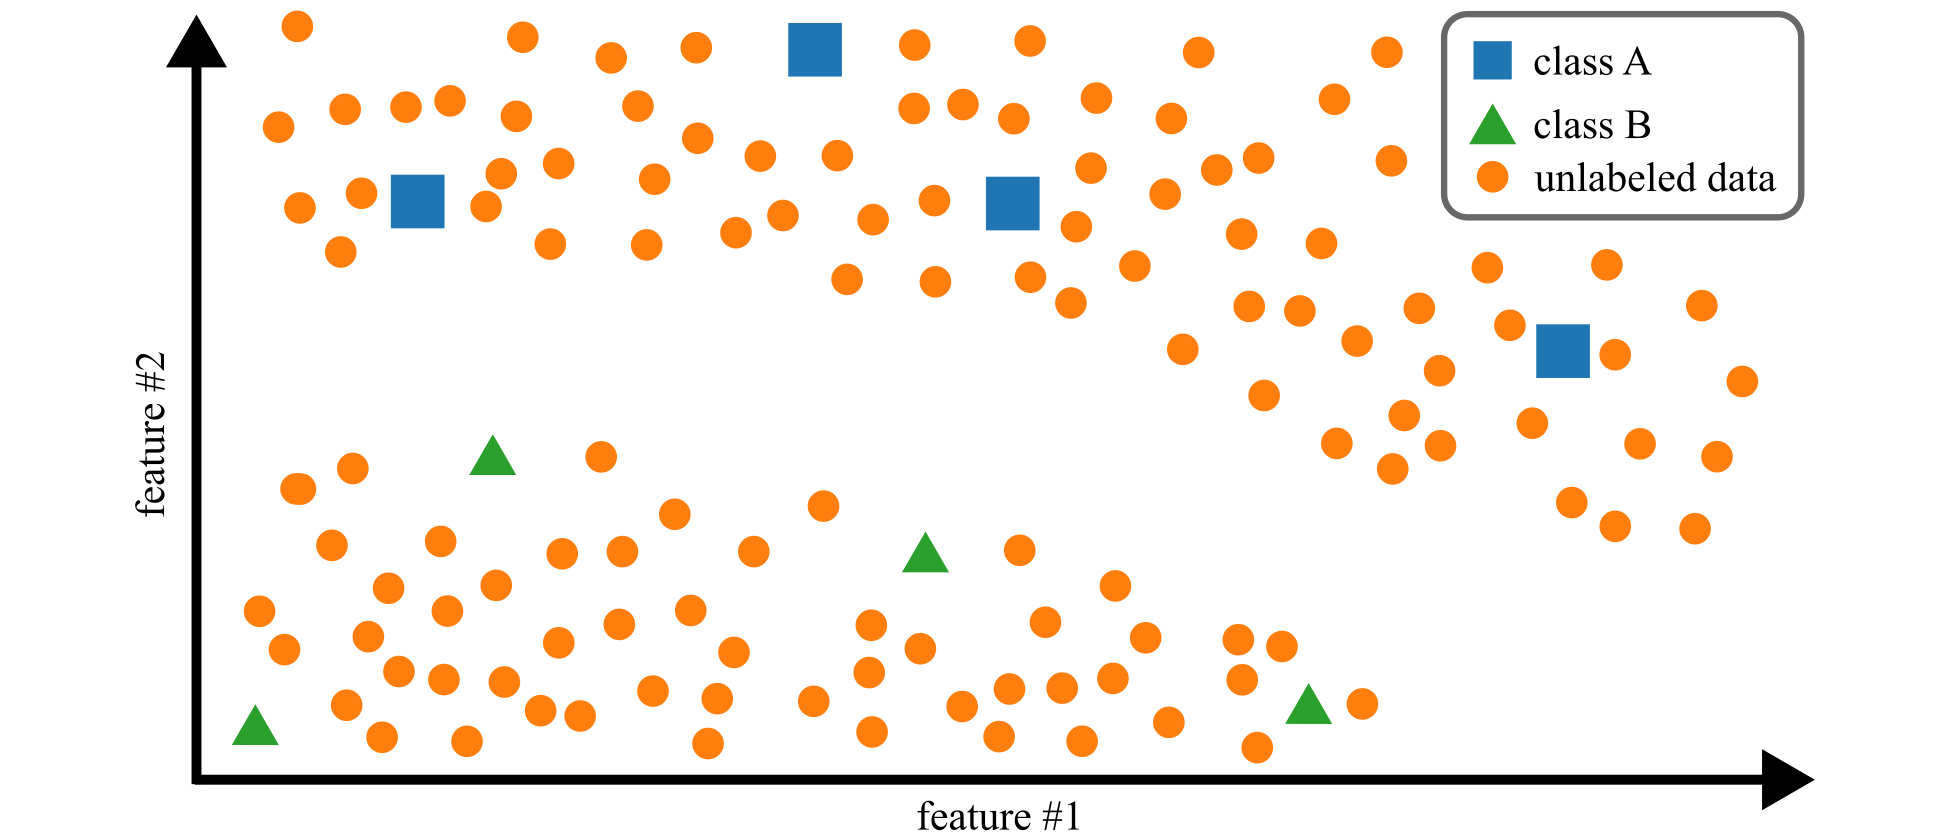
\includegraphics[width=\linewidth]{../figures/semisupervised_learning}
				\caption{Semisupervised learning enabling the use of a limited set of labeled data to infer the labels of larger unlabeled datasets.}
				\label{fig:semisupervised_learning}
			\end{figure}
		
		\subsubsection{Reinforcement Learning}
			
			Reinforcement learning follows a distinct paradigm in which an autonomous agent repeatedly interacts with its environment. At each step the agent observes the current state, chooses and executes an action, and then receives feedback in the form of a reward or penalty; as shown in figure~\ref{fig:reinforcement_learning_control_diagram}. By sampling many such cycles the agent gradually discovers a strategy, known as a policy, that maps perceived situations to actions so as to maximise the total reward accumulated over time.

			
%			\begin{ML_case_study}
%				
%			\textbf{Jean-Baptiste Mouret}
%				
%			\begin{itemize}
%				\item	Teaching creatures to walk
%				\item	\url{https://youtu.be/kQ2bqz3HPJE?t=58}
%				\item	Jean-Baptiste Mouret (2015) has been developing robots that give me nightmares. 
%				\item	The robot learns how to walk by ``searching'' a space to decide how to walk. 
%			\end{itemize}
%				
%			\end{ML_case_study}
%
%			\begin{ML_case_study}
%	
%			\textbf{Walking robots}
%				
%			\begin{itemize}
%				\item	\url{https://youtu.be/T-c17RKh3uE?t=23}
%				\item	It takes about 40 seconds for the robot to re-learn how to walk. It can be 96\% as fast with a broken leg. 
%			\end{itemize}
%						
%		\end{ML_case_study}		

			
			
			\begin{figure}[H]
				\centering
				
\includegraphics[width=\linewidth]{../figures/reinforcement_learning_control_diagram}
				\caption{reinforcement learning control diagram}
				\label{fig:reinforcement_learning_control_diagram}
			\end{figure}
			
			

	
	\subsection{Types of learning (Batch and Online)}
		
Machine learning systems can be broadly categorized based on how they process and learn from data.

%\todo{make figures for online and batch learning}


		\subsubsection{Batch Learning}
		
		

In batch learning, the system is fully trained using the entirety of the available data, which often demands significant time and computational resources, and is thus usually performed offline. Initially, the system undergoes training; after which, it is deployed into production where it no longer learns but merely applies the previously acquired knowledge. This method is referred to as offline learning. The deployment phase, known as inference, is typically executed swiftly.

To update a batch learning system with new information, such as recognizing a novel form of spam, it is necessary to develop a completely new version of the system. This version must be trained from the ground up using the entire dataset, both old and new data, before replacing the older system in production.

Despite these challenges, the training, evaluation, and deployment processes of a machine learning system can be automated, allowing even batch learning systems to adapt to changes. This approach is straightforward and usually effective; however, training on a full dataset can be time-consuming - often taking many hours - hence, systems are usually updated no more frequently than daily or weekly. Moreover, utilizing the full dataset requires extensive computing resources, such as CPU power, memory, disk space, and network bandwidth. For organizations with vast amounts of data, the costs of daily retraining from scratch can be prohibitively expensive.

If the dataset is exceptionally large, employing a batch learning algorithm may become impractical. Additionally, in situations where autonomous learning is essential and computational resources are limited, such as with smartphone applications or extraterrestrial rovers, the need to manage large datasets and conduct lengthy training sessions daily poses significant challenges.
		
		
		\subsubsection{Online Learning}

			
Online learning trains a model incrementally by presenting new data points one at a time or in small mini-batches. Each update is computationally light and fast, allowing the model to refresh its knowledge continuously as fresh data streams in. This approach is particularly appropriate for systems that:
\begin{itemize}[itemsep=0.25ex]
    \item receive data continuously, such as stock prices,
    \item need to quickly or autonomously adapt to changes,
    \item have limited computing resources: once an online learning system processes new data instances, they can be discarded to save space, unless there is a need to revert to a previous state and ``replay'' the data.
\end{itemize}
Online learning is also useful for managing large datasets that exceed the memory capacity of a single machine, known as out-of-core learning. The algorithm processes parts of the data, conducts a training step, and repeats this until all the data has been processed.

A critical parameter in online learning systems is the learning rate, which dictates how rapidly the system adapts to changing data. A high learning rate allows for rapid adaptation but may also lead to quick forgetting of old data and training on noise. A low learning rate results in slower learning and reduced sensitivity to variations in new data.

		
		\subsubsection{Bad Data in Machine Learning }
		\vspace{-1ex}		

		A significant challenge in online learning is the system's susceptibility to performance degradation when exposed to poor quality data. This is particularly problematic in live systems where clients might quickly notice issues. For instance, bad data could originate from a malfunctioning robot sensor or an attempt to manipulate search engine rankings through spamming. To mitigate these risks, it is crucial to vigilantly monitor the system and quickly disable learning or revert to a previously effective state if a decline in performance is observed. Additionally, monitoring the input data for anomalies and employing anomaly detection algorithms can help identify and respond to aberrant data.


			\begin{figure}[H]
				\centering
				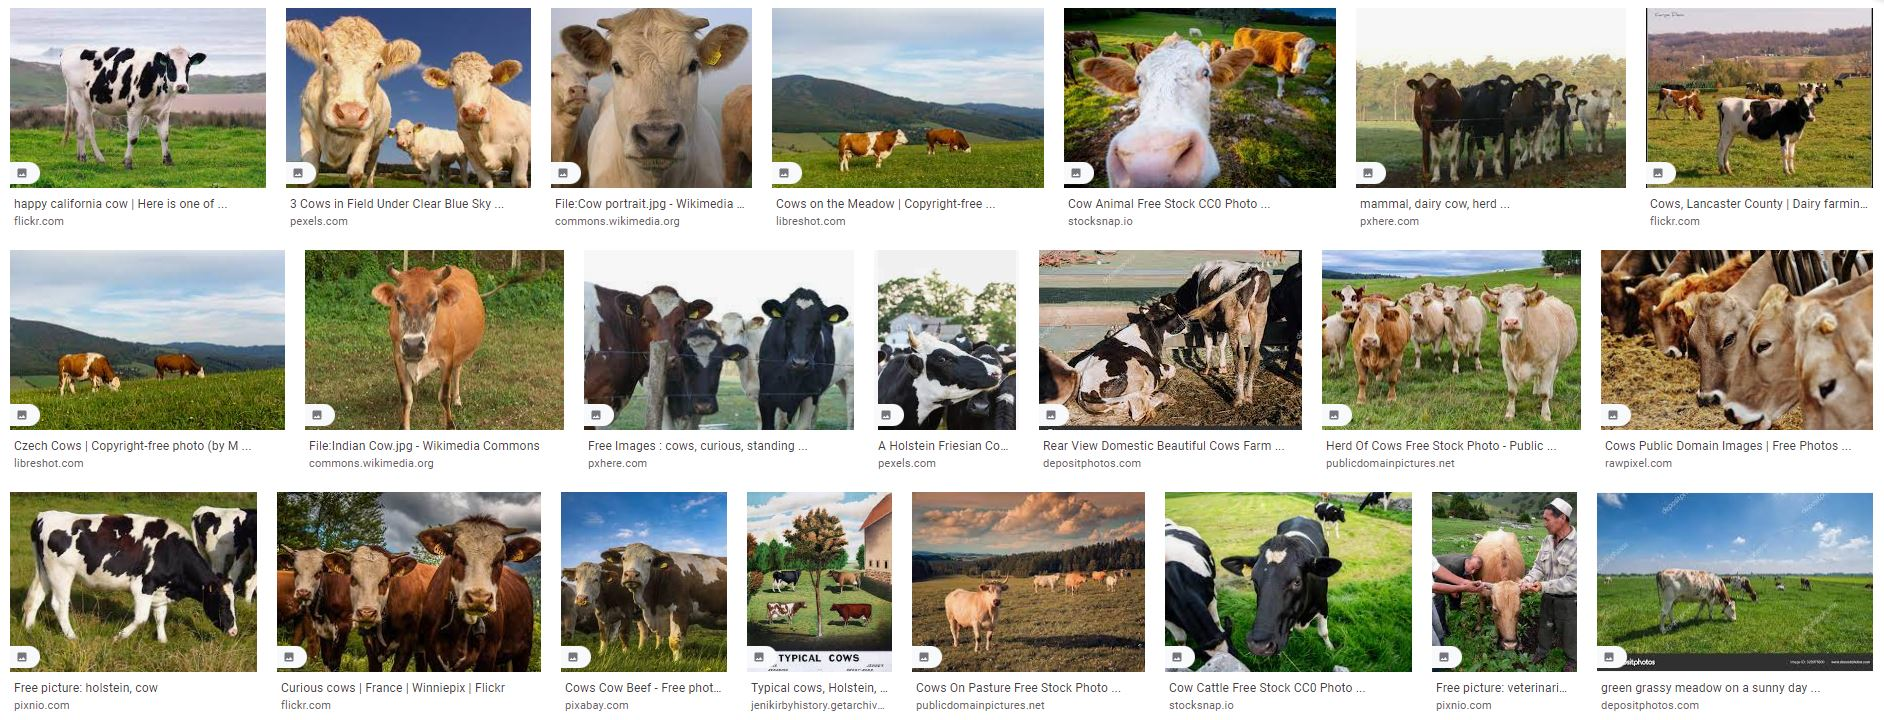
\includegraphics[width=6in]{../figures/cows}
				\vspace{-1ex}
				\caption{Training a machine learning algorithm to recognize cows may end up just learning to recognize grass. This is sometimes called ``short-cut learning''\protect\footnotemark[1].}
				\label{fig:cows}
			\end{figure}


			\footnotetext[1]{Screen shoot of a Google image search for cows taken by the Austin Downey, all images stated to be under a creative commons license per Google search tools; also assumed to be fair use under given the educational purpose of this text, via \url{https://www.google.com/}}


		For example, imagine training a convolutional neural network to recognize cows (Figure~\ref{fig:cows}). Every image in the training set shows black-and-white cattle standing on lush green pasture, so the easiest statistical cue for the model to latch onto is the dominant green background rather than the animals themselves. At inference time, the network confidently labels any scene filled with grass as ``cow,'' yet fails when presented with a cow on snow or asphalt. In other words, it has learned ``grass recognition,'' not ``cow recognition''.


		
	\subsection{Learning Approaches: Instance-Based and Model-Based}
		

Another method of classifying machine learning systems is based on their generalization capabilities. Typically, the main objective in machine learning is to make predictions, which requires the system to generalize from its training examples to new, unseen instances. Achieving high performance on training data is useful but not the ultimate goal; the system must also excel when confronted with new data.
There are primarily two strategies for generalization: instance-based learning and model-based learning.
		

\begin{figure}[H]
	\centering
	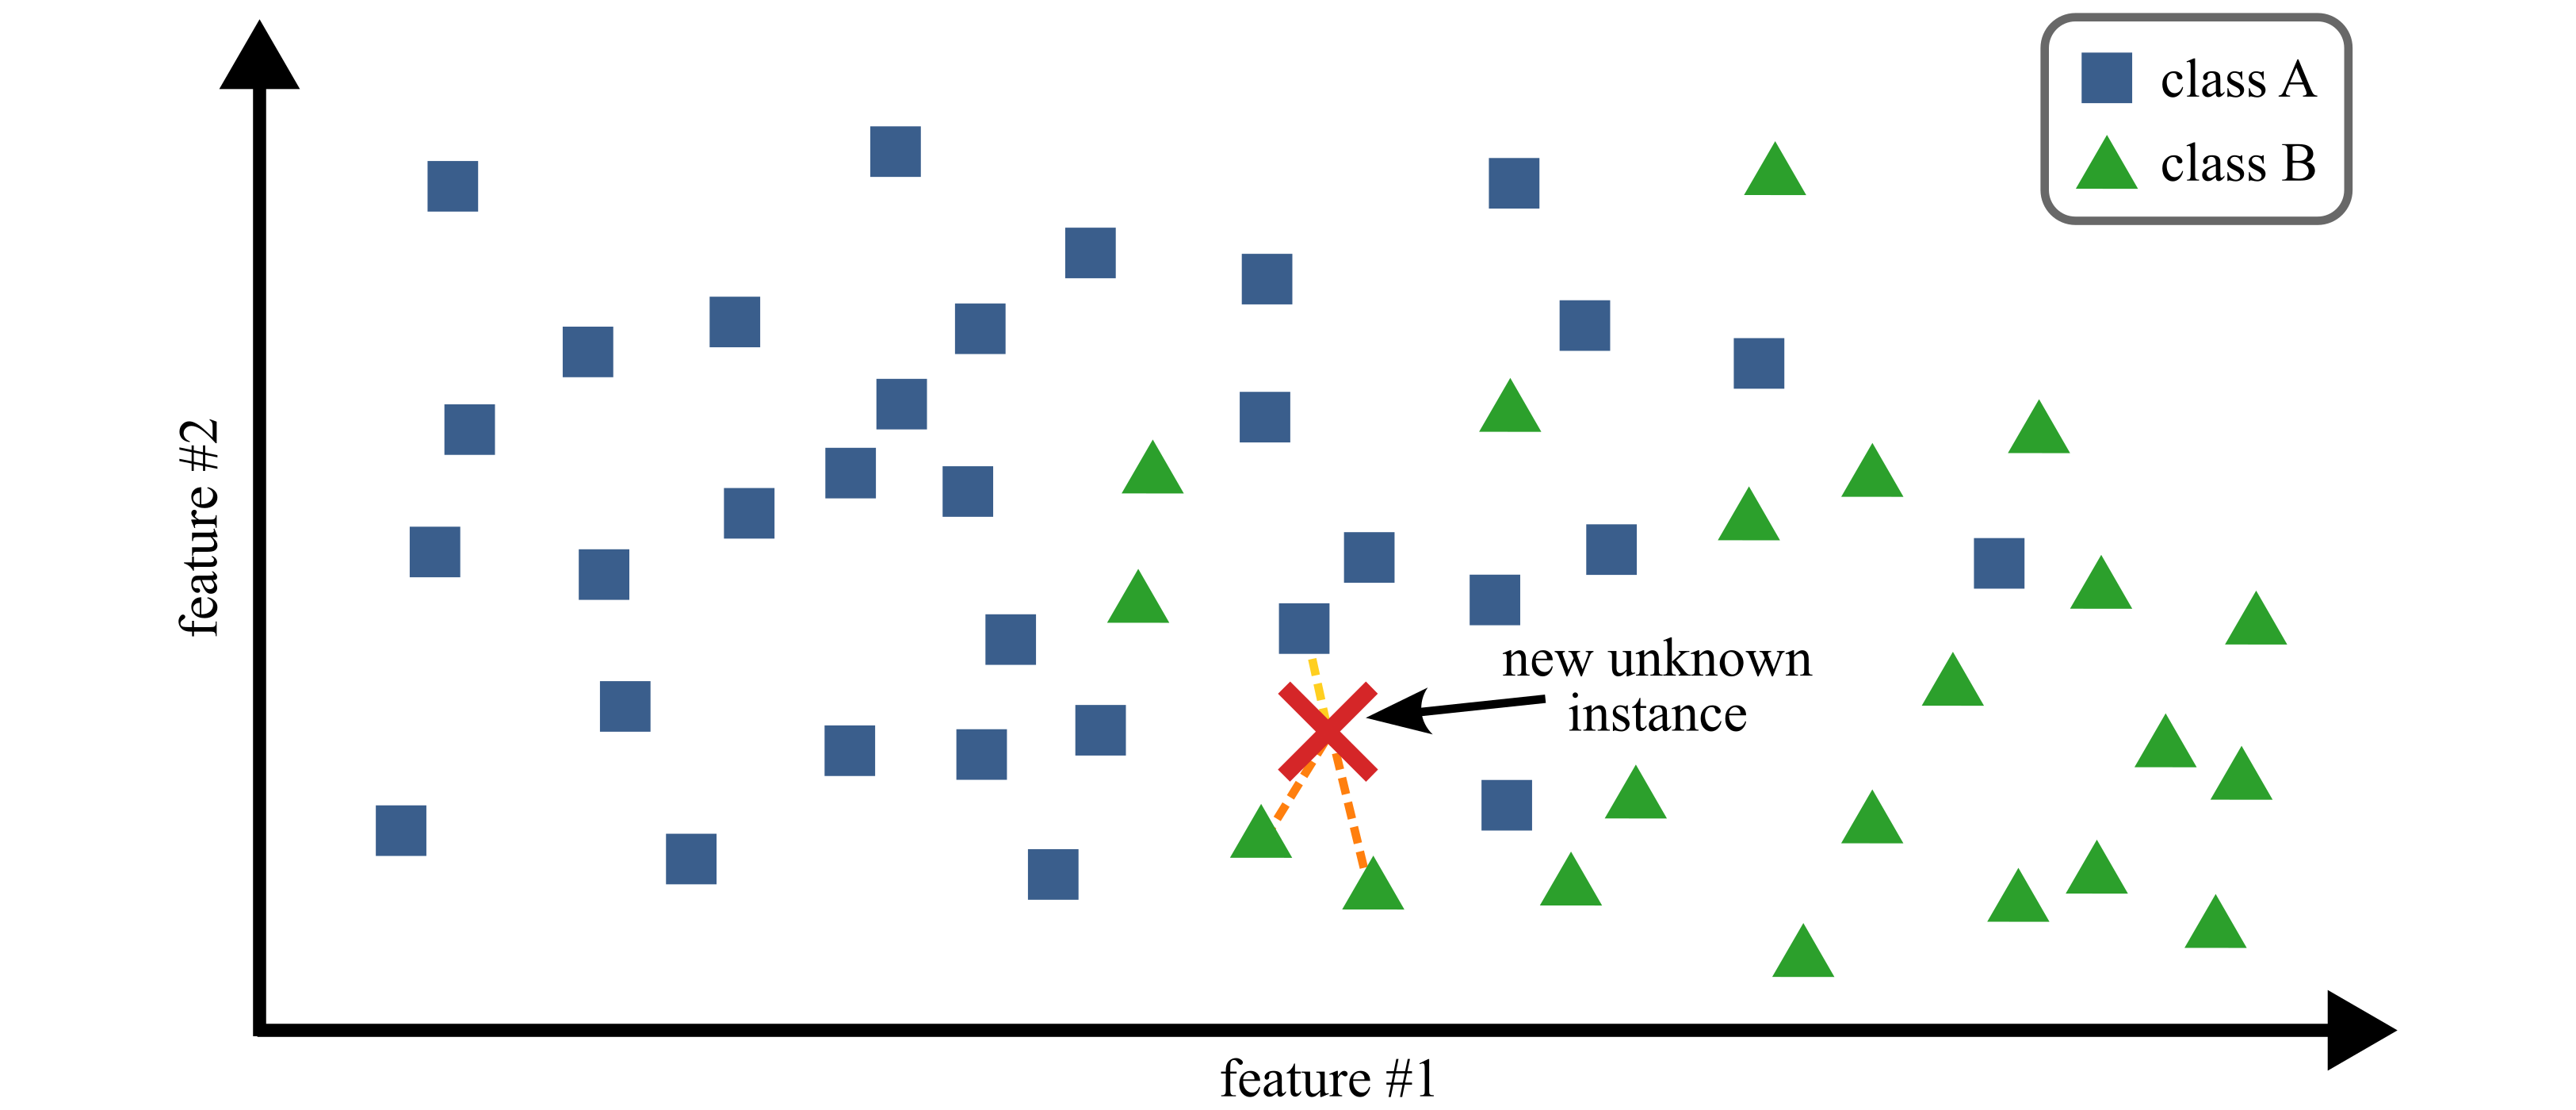
\includegraphics[width=\linewidth]{../figures/instance_based_learning}
	\caption{Instance-based learning where the class of a unknown instance is inferred from the its distance to data points with known labels.}
	\label{fig:instance_based_learning}
\end{figure}
		
		\subsubsection{Instance-based learning}
		

One of the simplest learning strategies is rote memorization. For instance, a spam filter built on this principle would only mark emails as spam if they match previously flagged emails exactly. While this approach is straightforward, it's hardly the most effective.
A more sophisticated spam filter could extend its detection capabilities to include emails that closely resemble known spam messages. This approach necessitates a metric for measuring the similarity between two emails. A basic method might involve counting the shared words between emails. Under this system, an email would be classified as spam if it shares a significant number of words with an email already identified as spam.
This method exemplifies instance-based learning (Figure~\ref{fig:instance_based_learning}), where the system memorizes specific examples and uses a similarity metric to generalize to new instances.
			
			

		\pagebreak
		
		\subsubsection{Model-based learning}
				\vspace{-1ex}
		
Another approach to generalization involves constructing a model based on a set of examples and then using this model to make predictions as shown in figure~\ref{fig:model_based_learning}. This method is known as model-based learning.
			
			
			\begin{figure}[H]
			\centering
				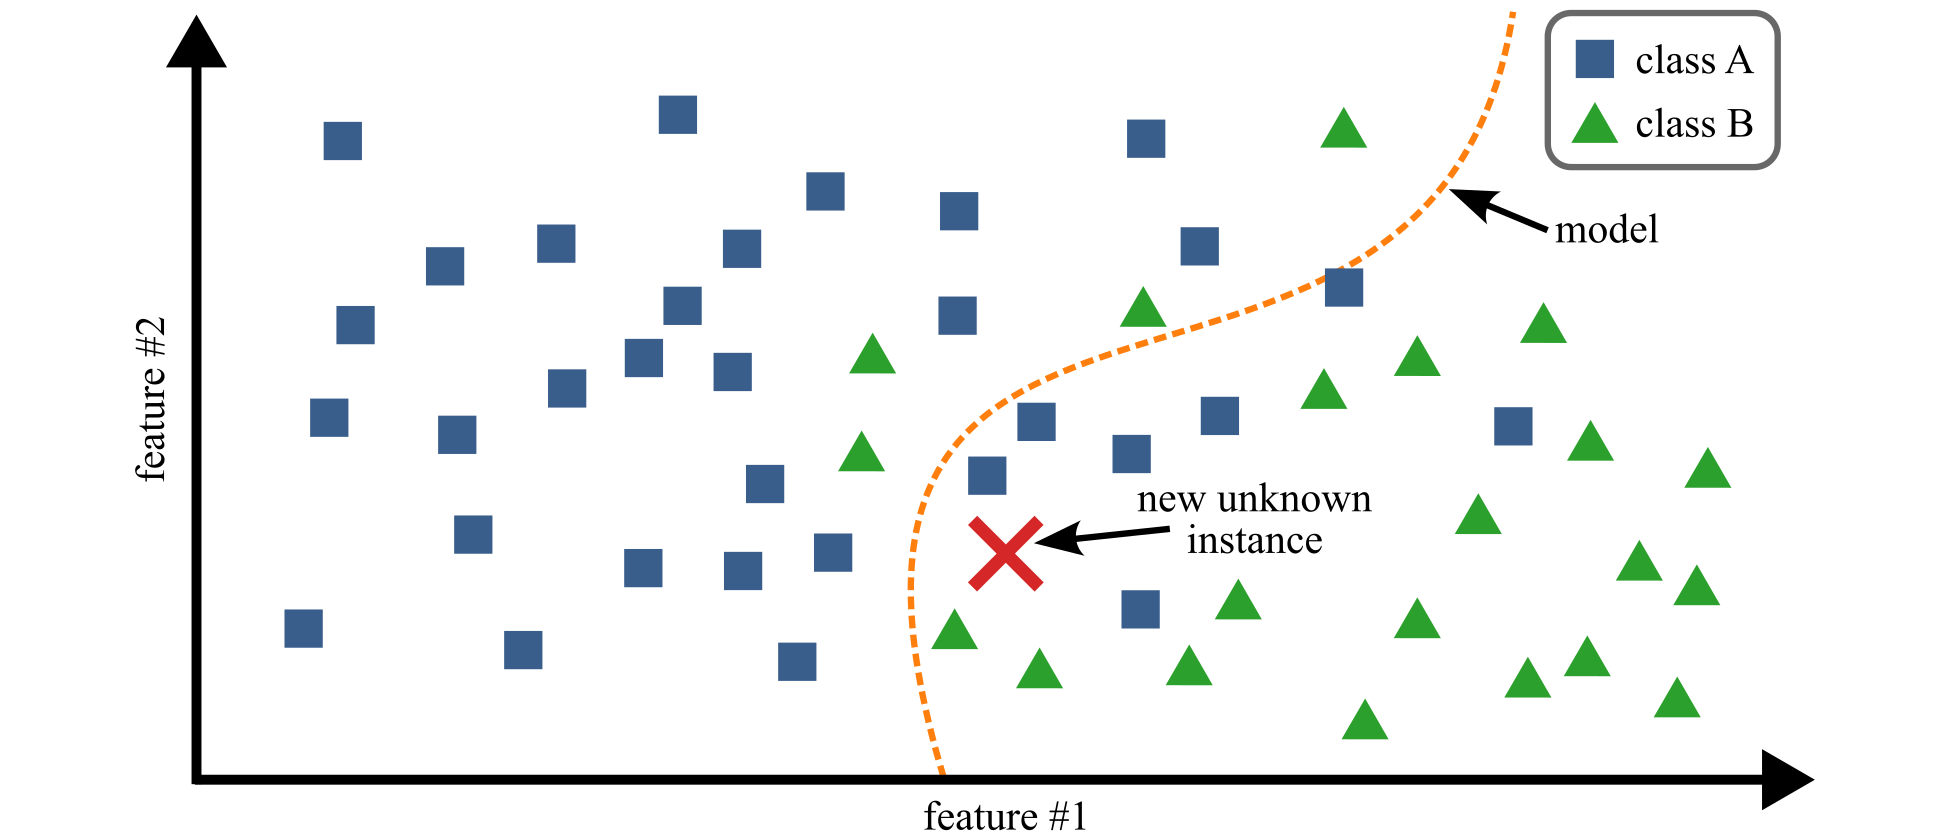
\includegraphics[width=6in]{../figures/model_based_learning}
				\caption{Model-based learning where the class of a unknown instance is inferred from its location in reference to a model trained on the data with known labels.}
				\label{fig:model_based_learning}
			\end{figure}
		
	
			\begin{figure}[H]
			\centering
				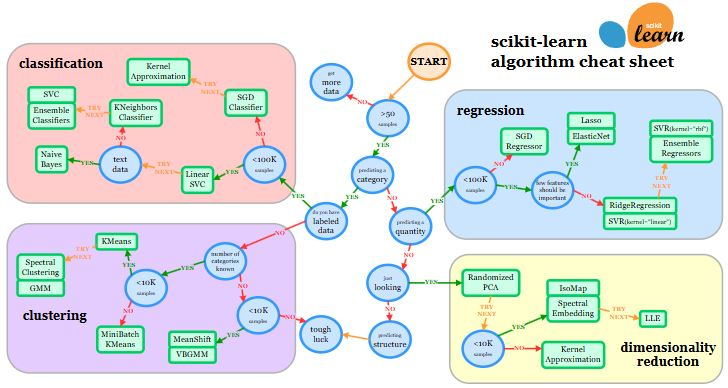
\includegraphics[width=6in]{../figures/ml_map}
				\caption{Flowchart of estimators used in the scikit learn library that intends guide users for what algorithms to use for a given case\protect\footnotemark[1].}
				\label{fig:ml_map}
			\end{figure}
			\footnotetext[1]{Scikit-learn algorithms cheat sheet, permissive simplified BSD license and assumed to be fair use under given its nature as documentation and the educational purpose of this text, via \url{https://scikit-learn.org/stable/tutorial/machine_learning_map/index.html}}
	
	
		\subsubsection{Selecting methods:}	


One of the initial challenges faced by newcomers to machine learning is selecting the appropriate algorithms (or estimators) for specific tasks. This is due to the fact that various algorithms excel with different kinds of data and problems. The flowchart depicted in Fig.~\ref{fig:ml_map}, which originates from the scikit-learn library documentation, is intended to guide users in choosing the most suitable algorithms for their particular datasets.


				\vspace{-1ex}
		\subsection{The Unreasonable Effectiveness of Data}
				\vspace{-1ex}

In a landmark study released in 2001, Microsoft researchers Michele Banko and Eric Brill demonstrated that a variety of Machine Learning algorithms, even relatively straightforward ones, achieved similar levels of performance on a complex task of natural language disambiguation when provided with sufficient data. This finding is illustrated in figure~\ref{fig:data_versus_algorithms} and further discussed in their paper\protect\footnotemark[1].

\footnotetext[1]{Michele Banko and Eric Brill. ``Scaling to very very large corpora for natural language disambiguation.'' Proceedings of the 39th annual meeting of the Association for Computational Linguistics. 2001.}

\begin{figure}[H]
\centering
	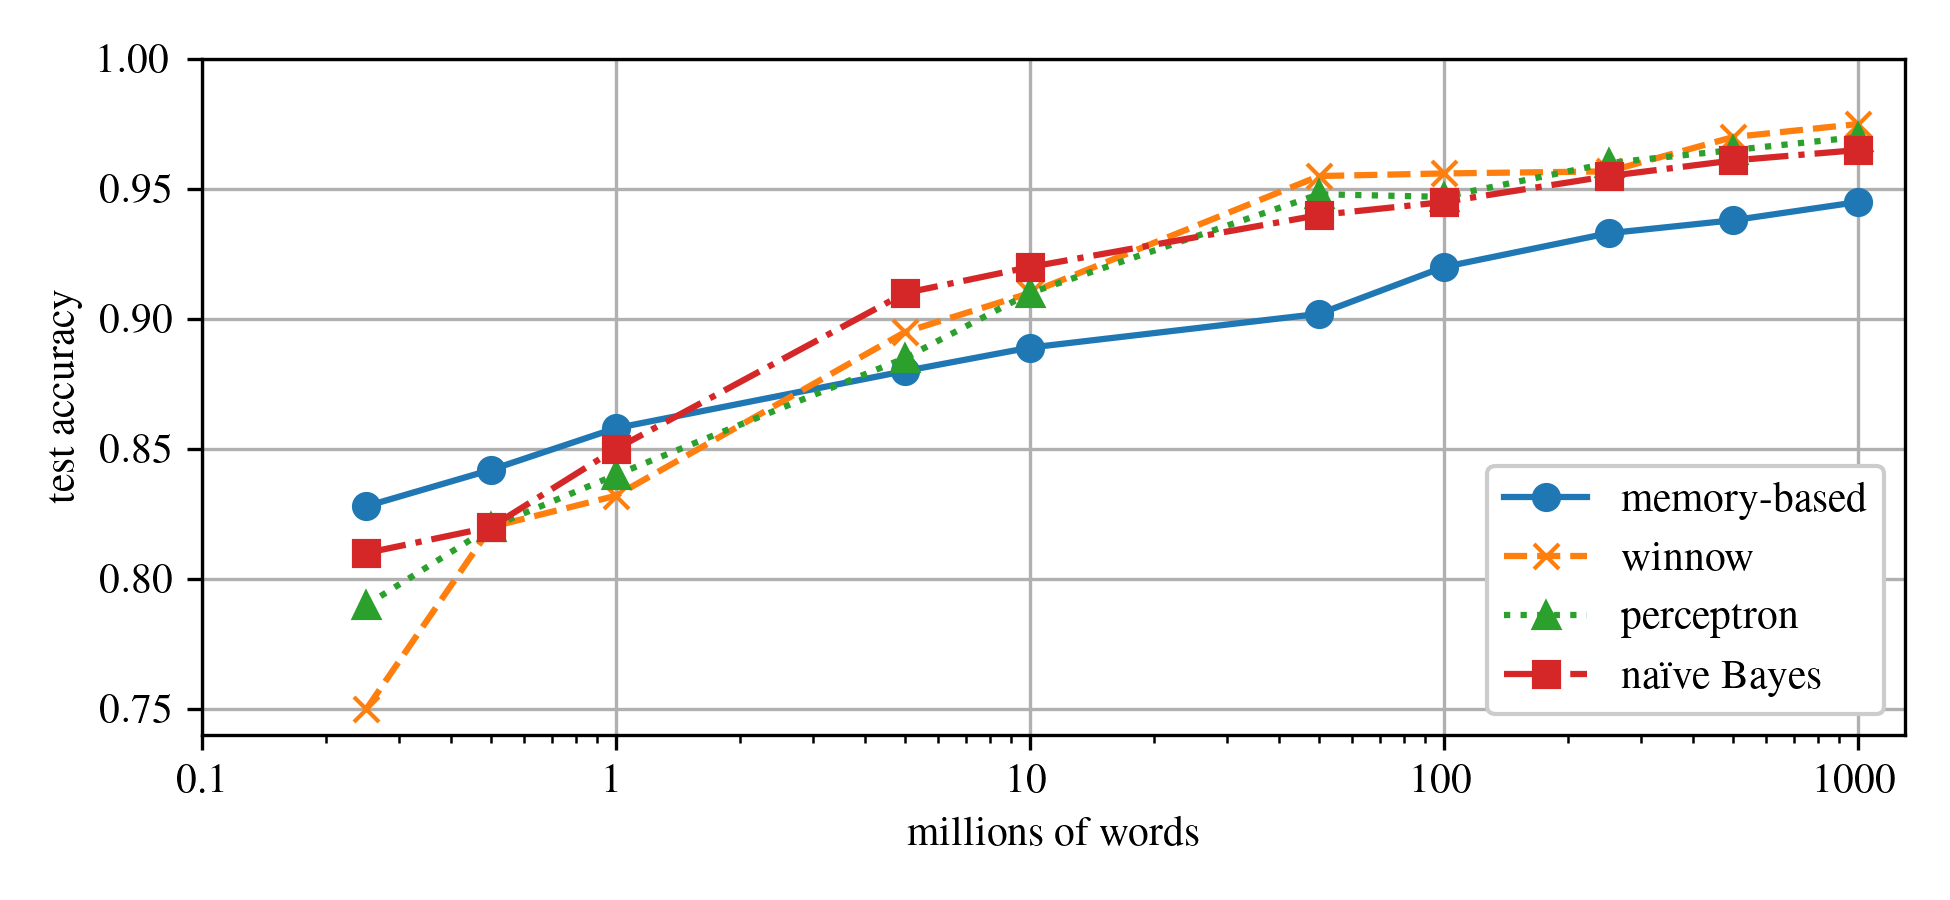
\includegraphics[width=6.5in]{../figures/data_versus_algorithms.png}
	\vspace{-2ex}
	\caption{Learning curves for four algorithms studied in Banko and Brill showing the importance of the amount of data when compared to algorithm selection.  }
	\label{fig:data_versus_algorithms}
\end{figure}


As the authors put it: ``these results suggest that we may want to reconsider the tradeoff between spending time and money on algorithm development versus spending it on corpus development.''. Or put more directly ``The Unreasonable Effectiveness of Data''\protect\footnotemark[2]. It's important to recognize, however, that small and medium-sized datasets remain prevalent, and acquiring additional training data is not always straightforward or economical. Therefore, the significance of algorithm selection should not be overlooked.

\footnotetext[2]{Halevy, Alon, Peter Norvig, and Fernando Pereira. ``The unreasonable effectiveness of data.'' IEEE intelligent systems 24.2 (2009): 8-12.}


\end{document}



% Chapter 2 Regression
\documentclass[12pt,letter]{article}
\usepackage{../downey_format}

\begin{document}
	
	% set the section number, along with figure and equation numbers
	\setcounter{section}{1}	
	\setcounter{figure}{0}   
	\renewcommand\thefigure{\thesection.\arabic{figure}}
	\setcounter{equation}{0}   
	\renewcommand\theequation{\thesection.\arabic{equation}}
	\section{Regression}


Regression is a fundamental tool in machine learning used to model the relationship between an independent variable (called data and denoted $x$) and a dependent variable (called target and denoted $y$). The goal is to learn a function that best predicts the target value from the input data. This relationship is shown in figure~\ref{fig:general_regression} .

\begin{figure}[H]
	\centering
	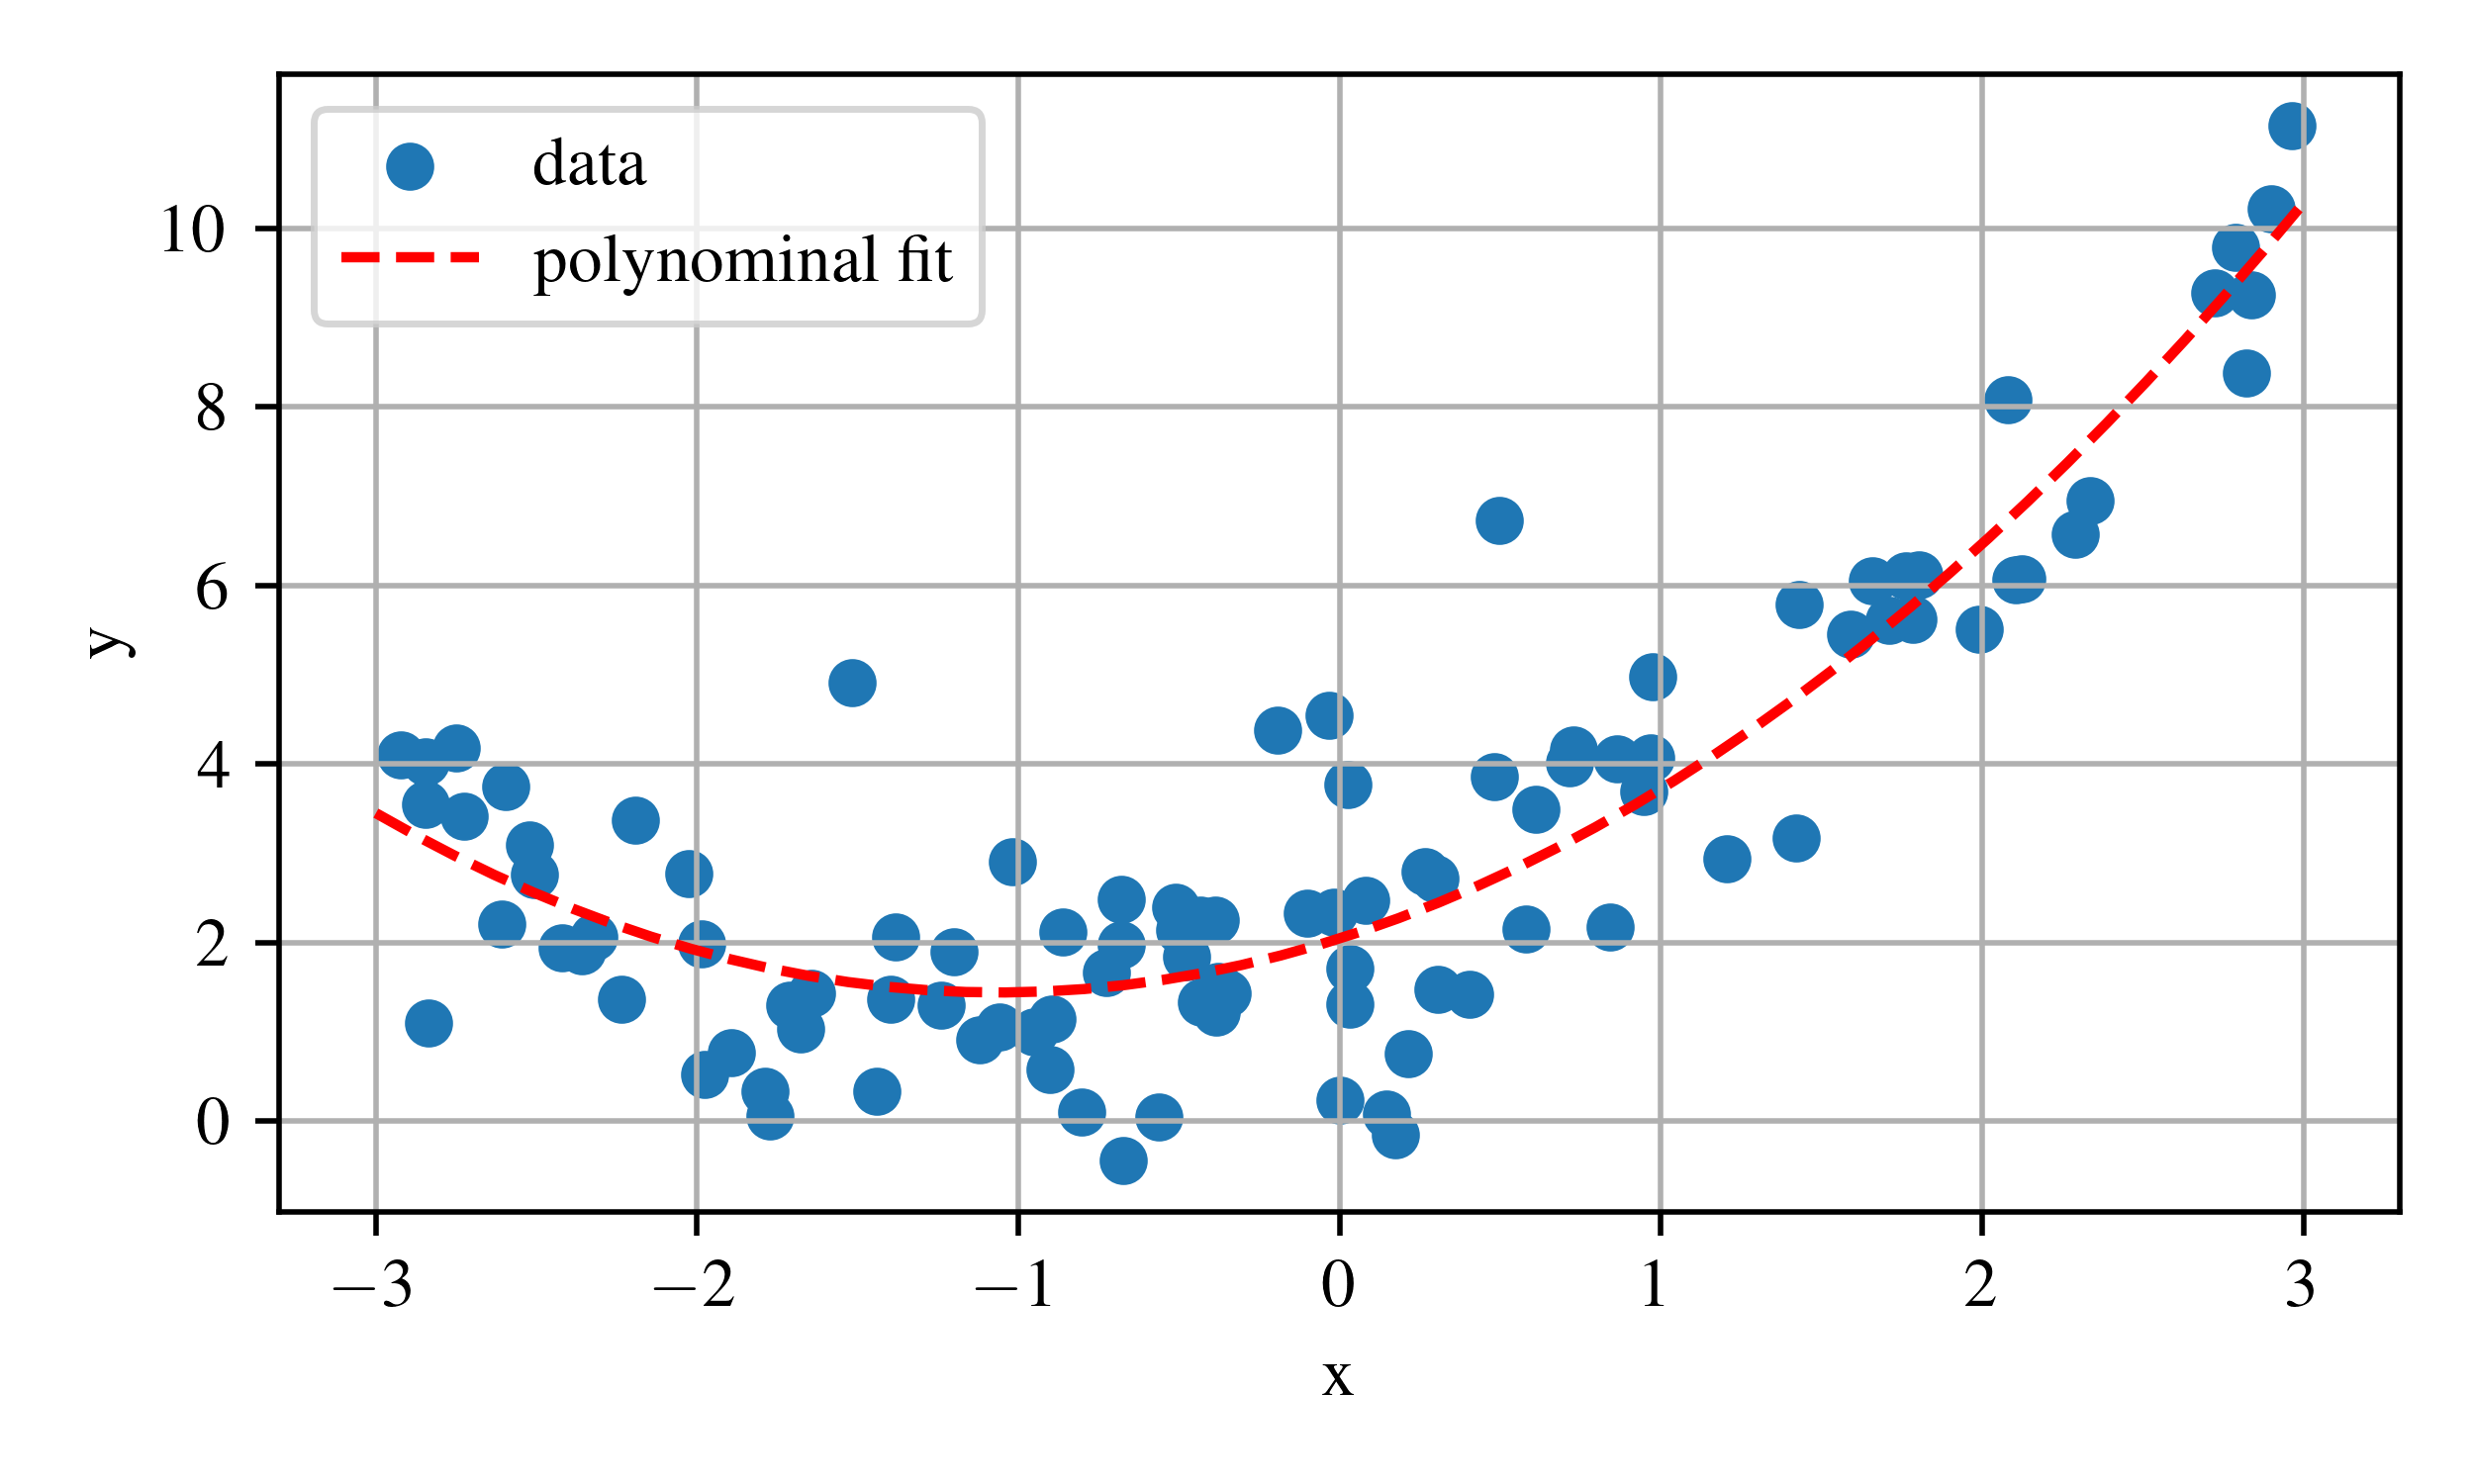
\includegraphics[width=4in]{../figures/polynomial_regression_3}
	\caption{Polynomial model fit via regression to a generic dataset. }
	\label{fig:general_regression}
\end{figure}
% \todo{need to update figure, add labels on x and y, get some sor of s-shaped data.}

In this chapter, we first examine Linear Regression and contrast two ways to estimate its parameters:
\begin{enumerate}
\item \textbf{Closed-form solution.} Solve for the parameter vector in one step by minimizing the cost function on the entire training set.  
\item \textbf{Gradient Descent .} Apply an iterative optimizer that repeatedly updates the parameters in small steps that lower the cost until it reaches the same optimum found by the closed-form method. We will look at three common Gradient Descent variants: Batch Gradient Descent, Mini-batch Gradient Descent, and Stochastic Gradient Descent.
\end{enumerate}
The first approach gives an exact answer immediately, whereas the second reaches that answer through successive refinements.





\begin{data}

	\textbf{Ames Housing Dataset}

	\noindent The Ames housing dataset provides details on individual residential property sales in Ames, Iowa, from 2006 to 2010 \protect\footnotemark[1]. It includes 2,930 entries and numerous variables (23 nominal, 23 ordinal, 14 discrete, and 20 continuous) that are used to evaluate home values \protect\footnotemark[2].
	
	\footnotetext[1]{The author of this text bought a home in Ames Iowa during this time right as the 2008 housing crash unfolded and on the last day they allowed home loans with no down payment.}
	\footnotetext[2]{De Cock, Dean. ``Ames, Iowa: Alternative to the Boston housing data as an end of semester regression project.'' Journal of Statistics Education 19.3 (2011).}
	%\footnotetext[2]{De Cock, Dean. ``Ames, Iowa: Alternative to the Boston housing data as an end of semester regression project.'' Journal of Statistics Education 19.3 (2011).}
	
	\begin{figure}[H]
		\centering
		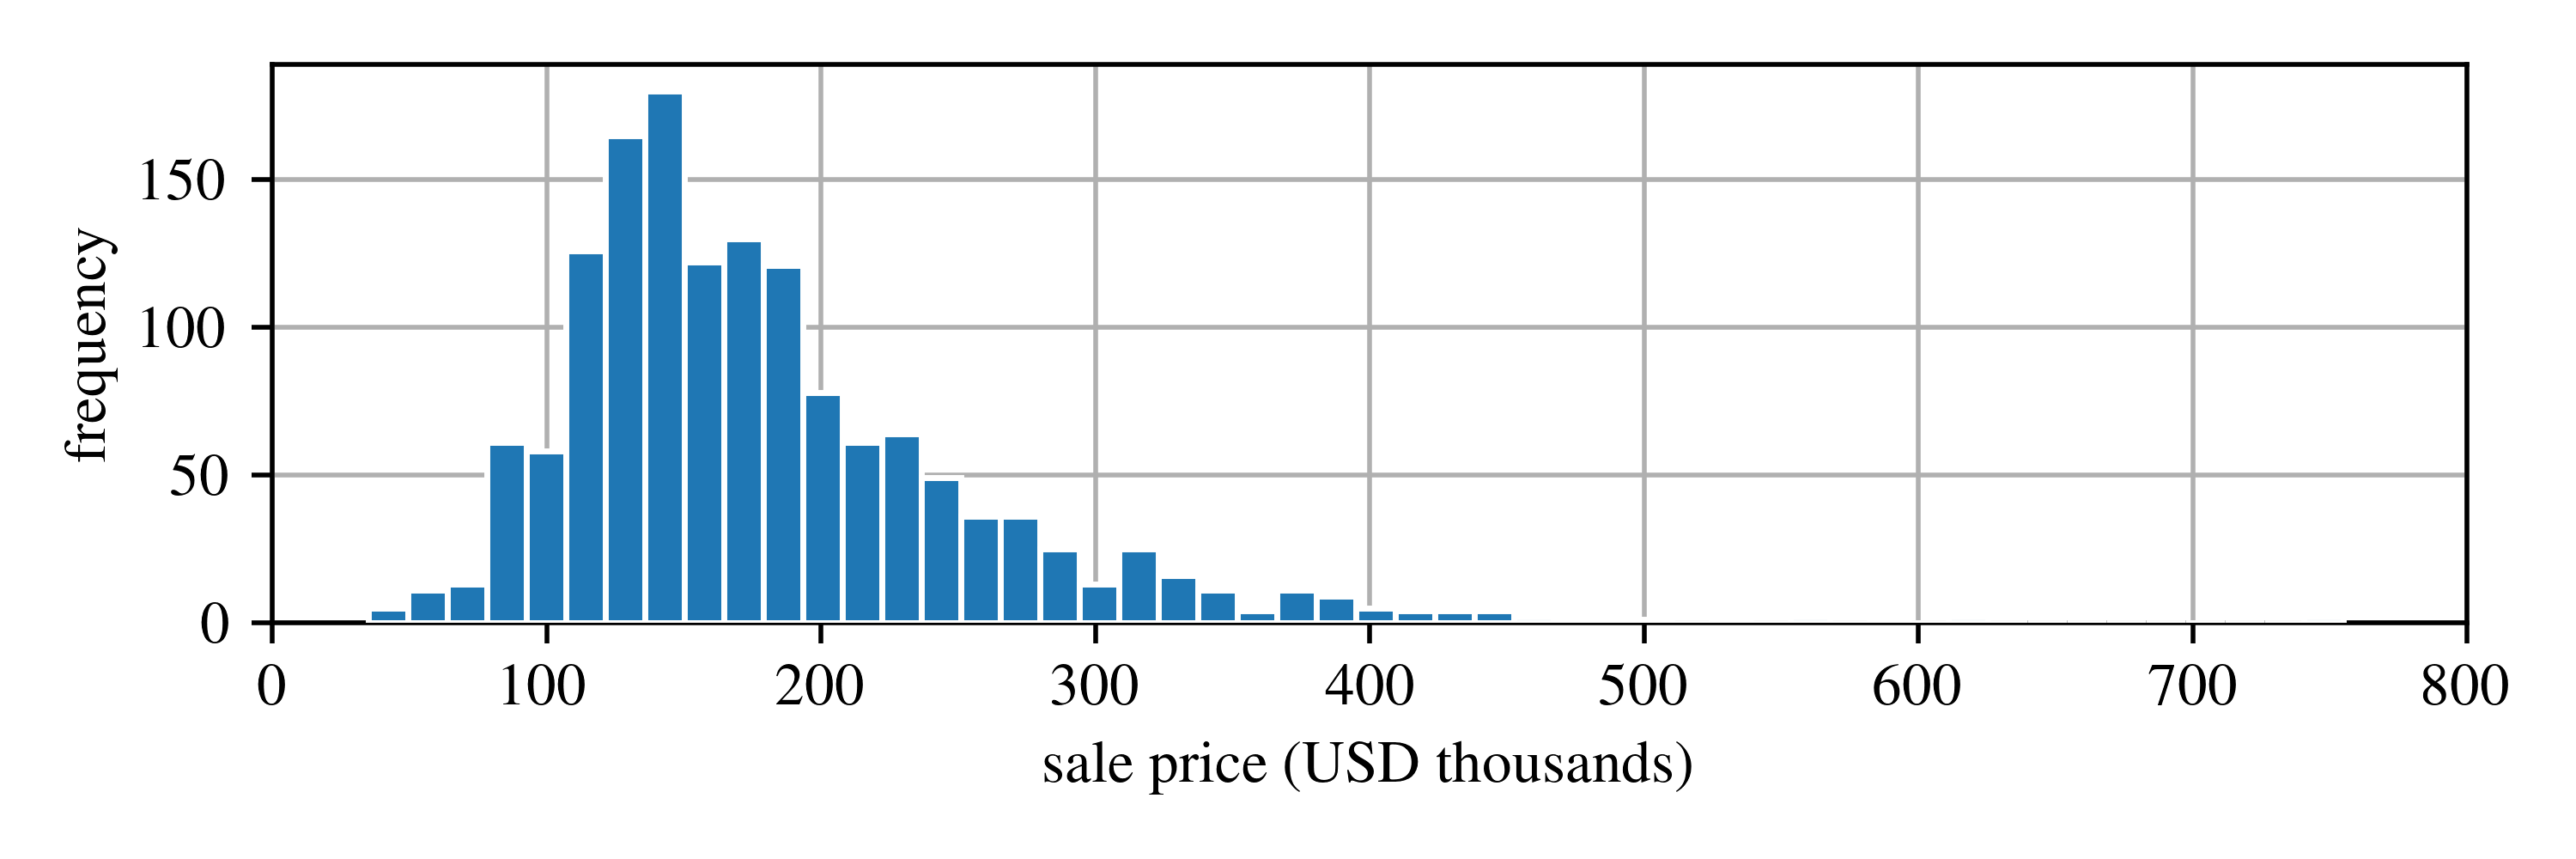
\includegraphics[width=5in]{../figures/Ames_histogram}
		\caption{Histogram of sale prices from 2006 to 2010 for the 2,930 entries.}
		\label{fig:Ames_histogram}
	\end{figure}
	
	\begin{figure}[H]
		\centering
		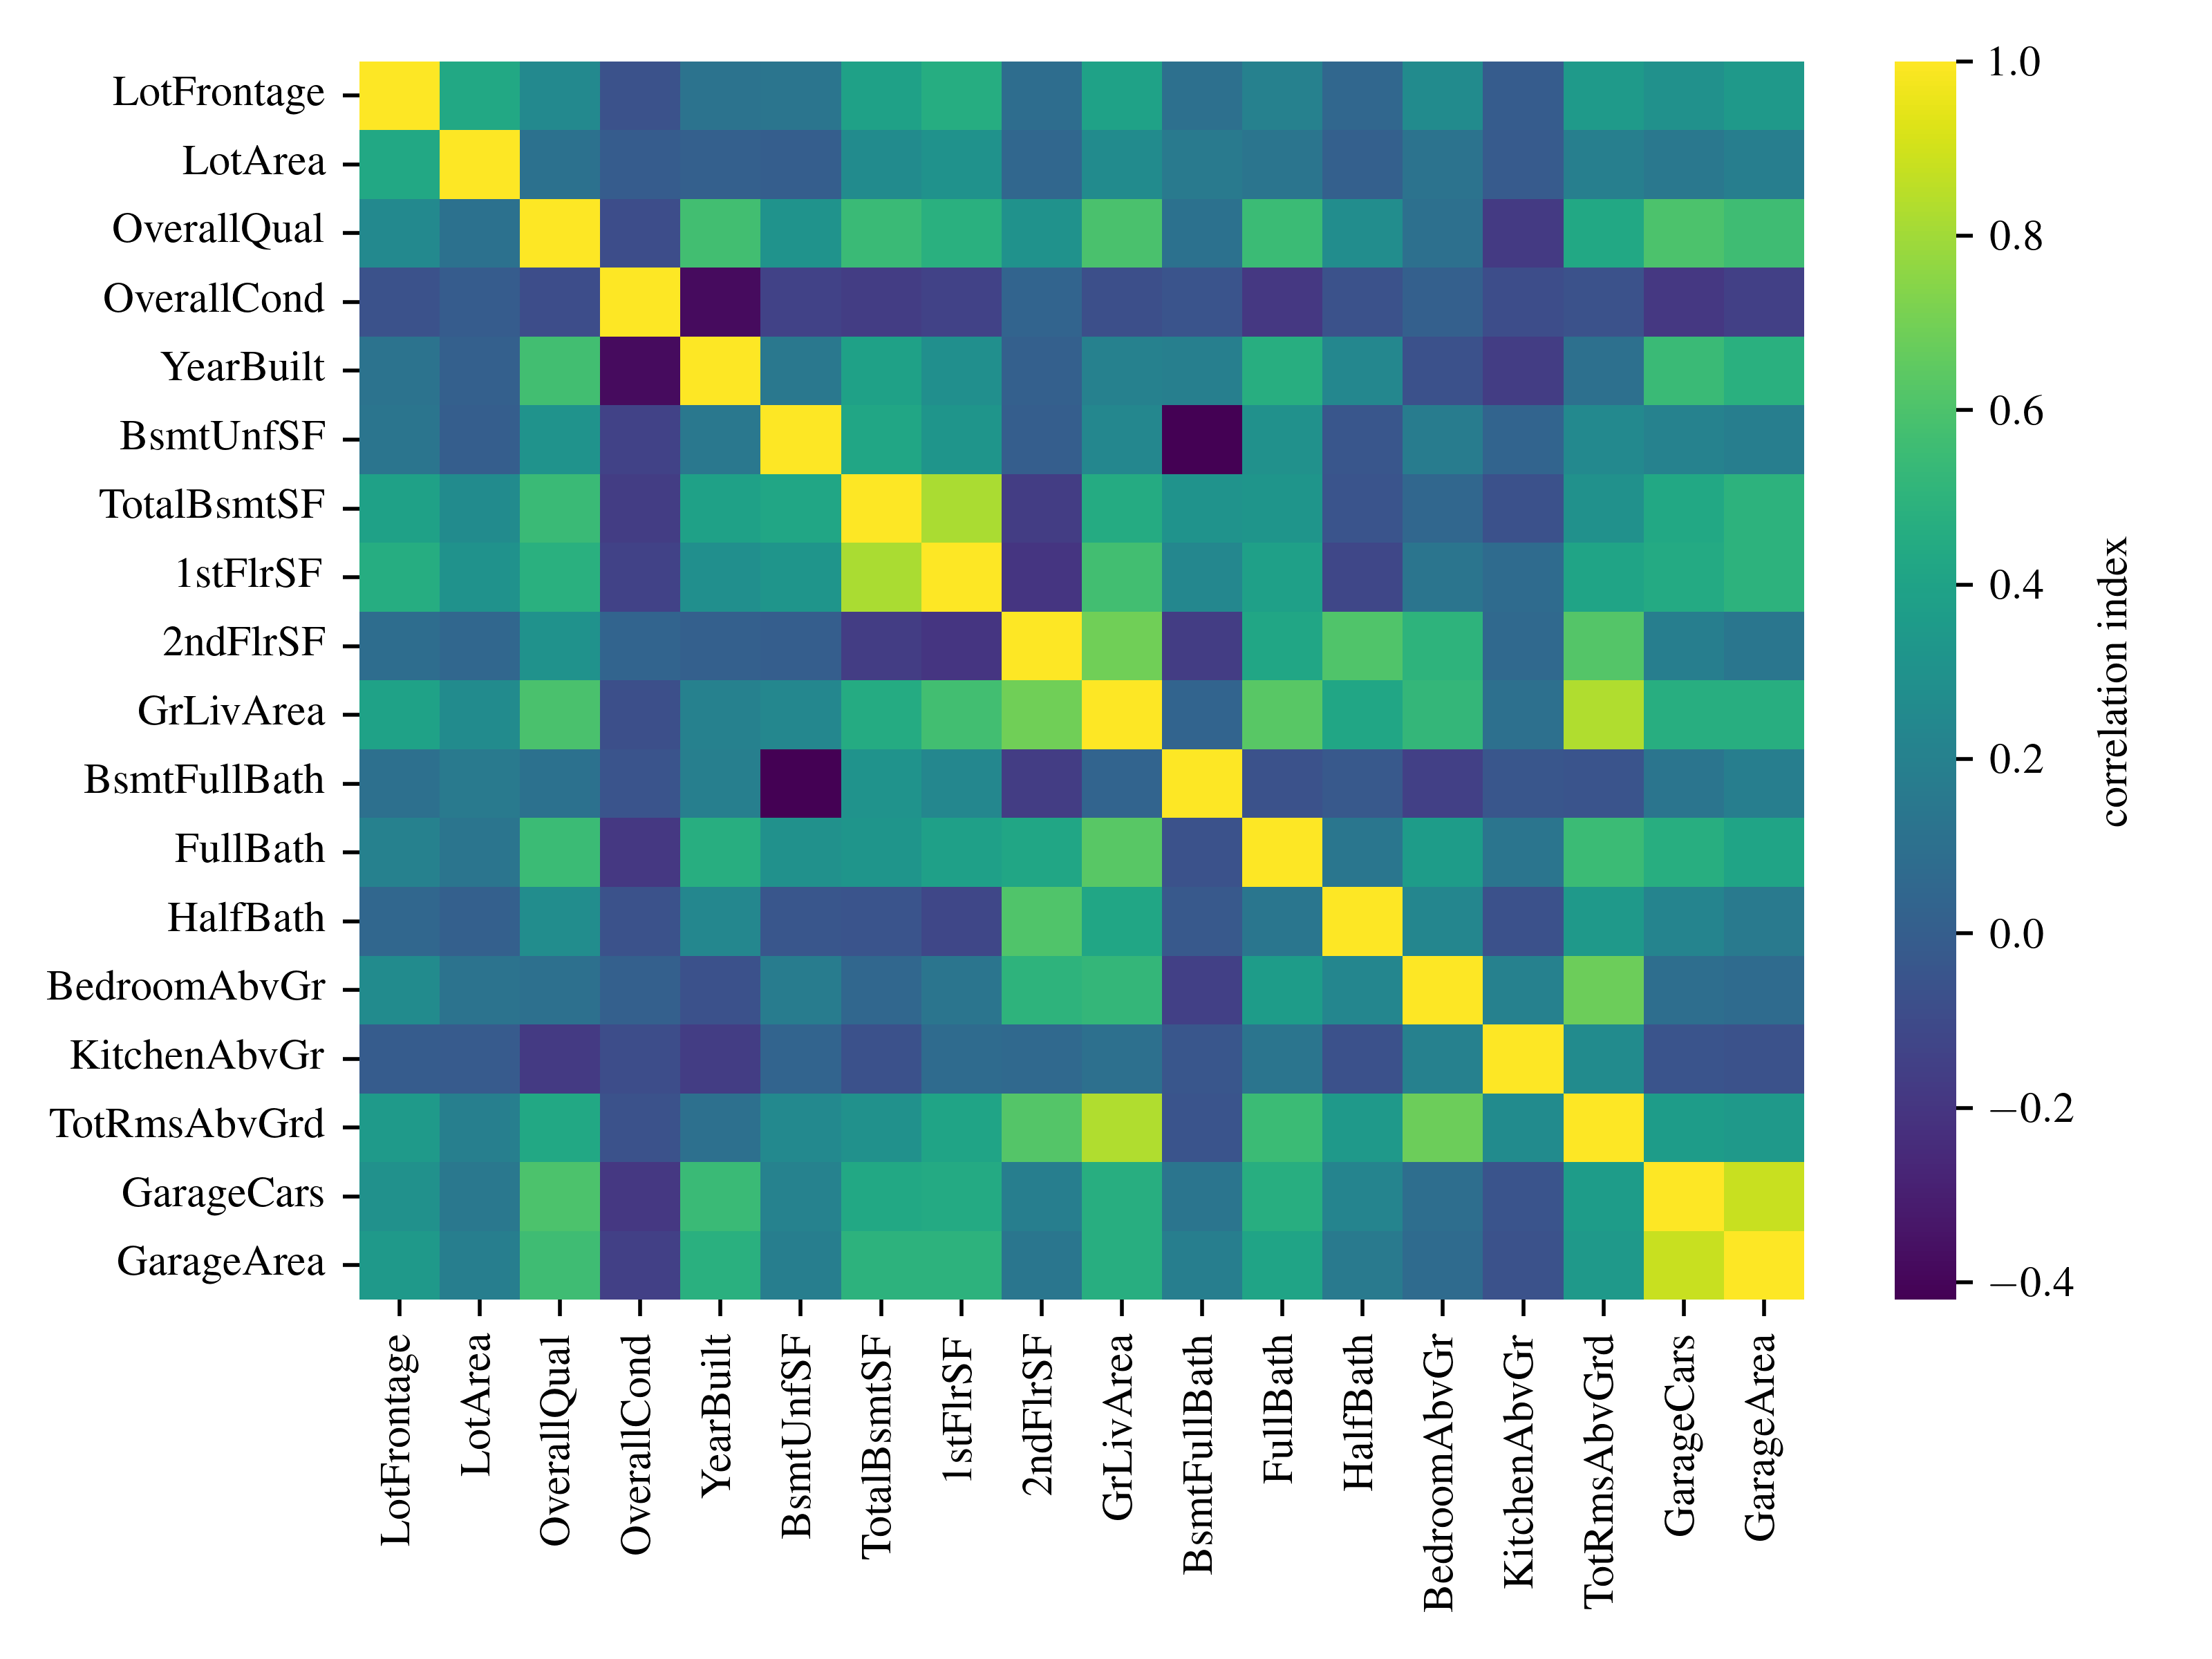
\includegraphics[width=5in]{../figures/Ames_housing_correlation_matirx}
		\caption{Correlation matrix for the 13 input parameters.}
		\label{fig:Ames_housing_correlation_matirx}
	\end{figure}

\end{data}





\subsection{Linear Regression}



Consider the scenario where you wish to determine the value of a house in Ames using the Ames dataset included in sklearn. To illustrate this, let us plot the relationship between the above ground living area and the housing price.

\begin{figure}[H]
    \centering
    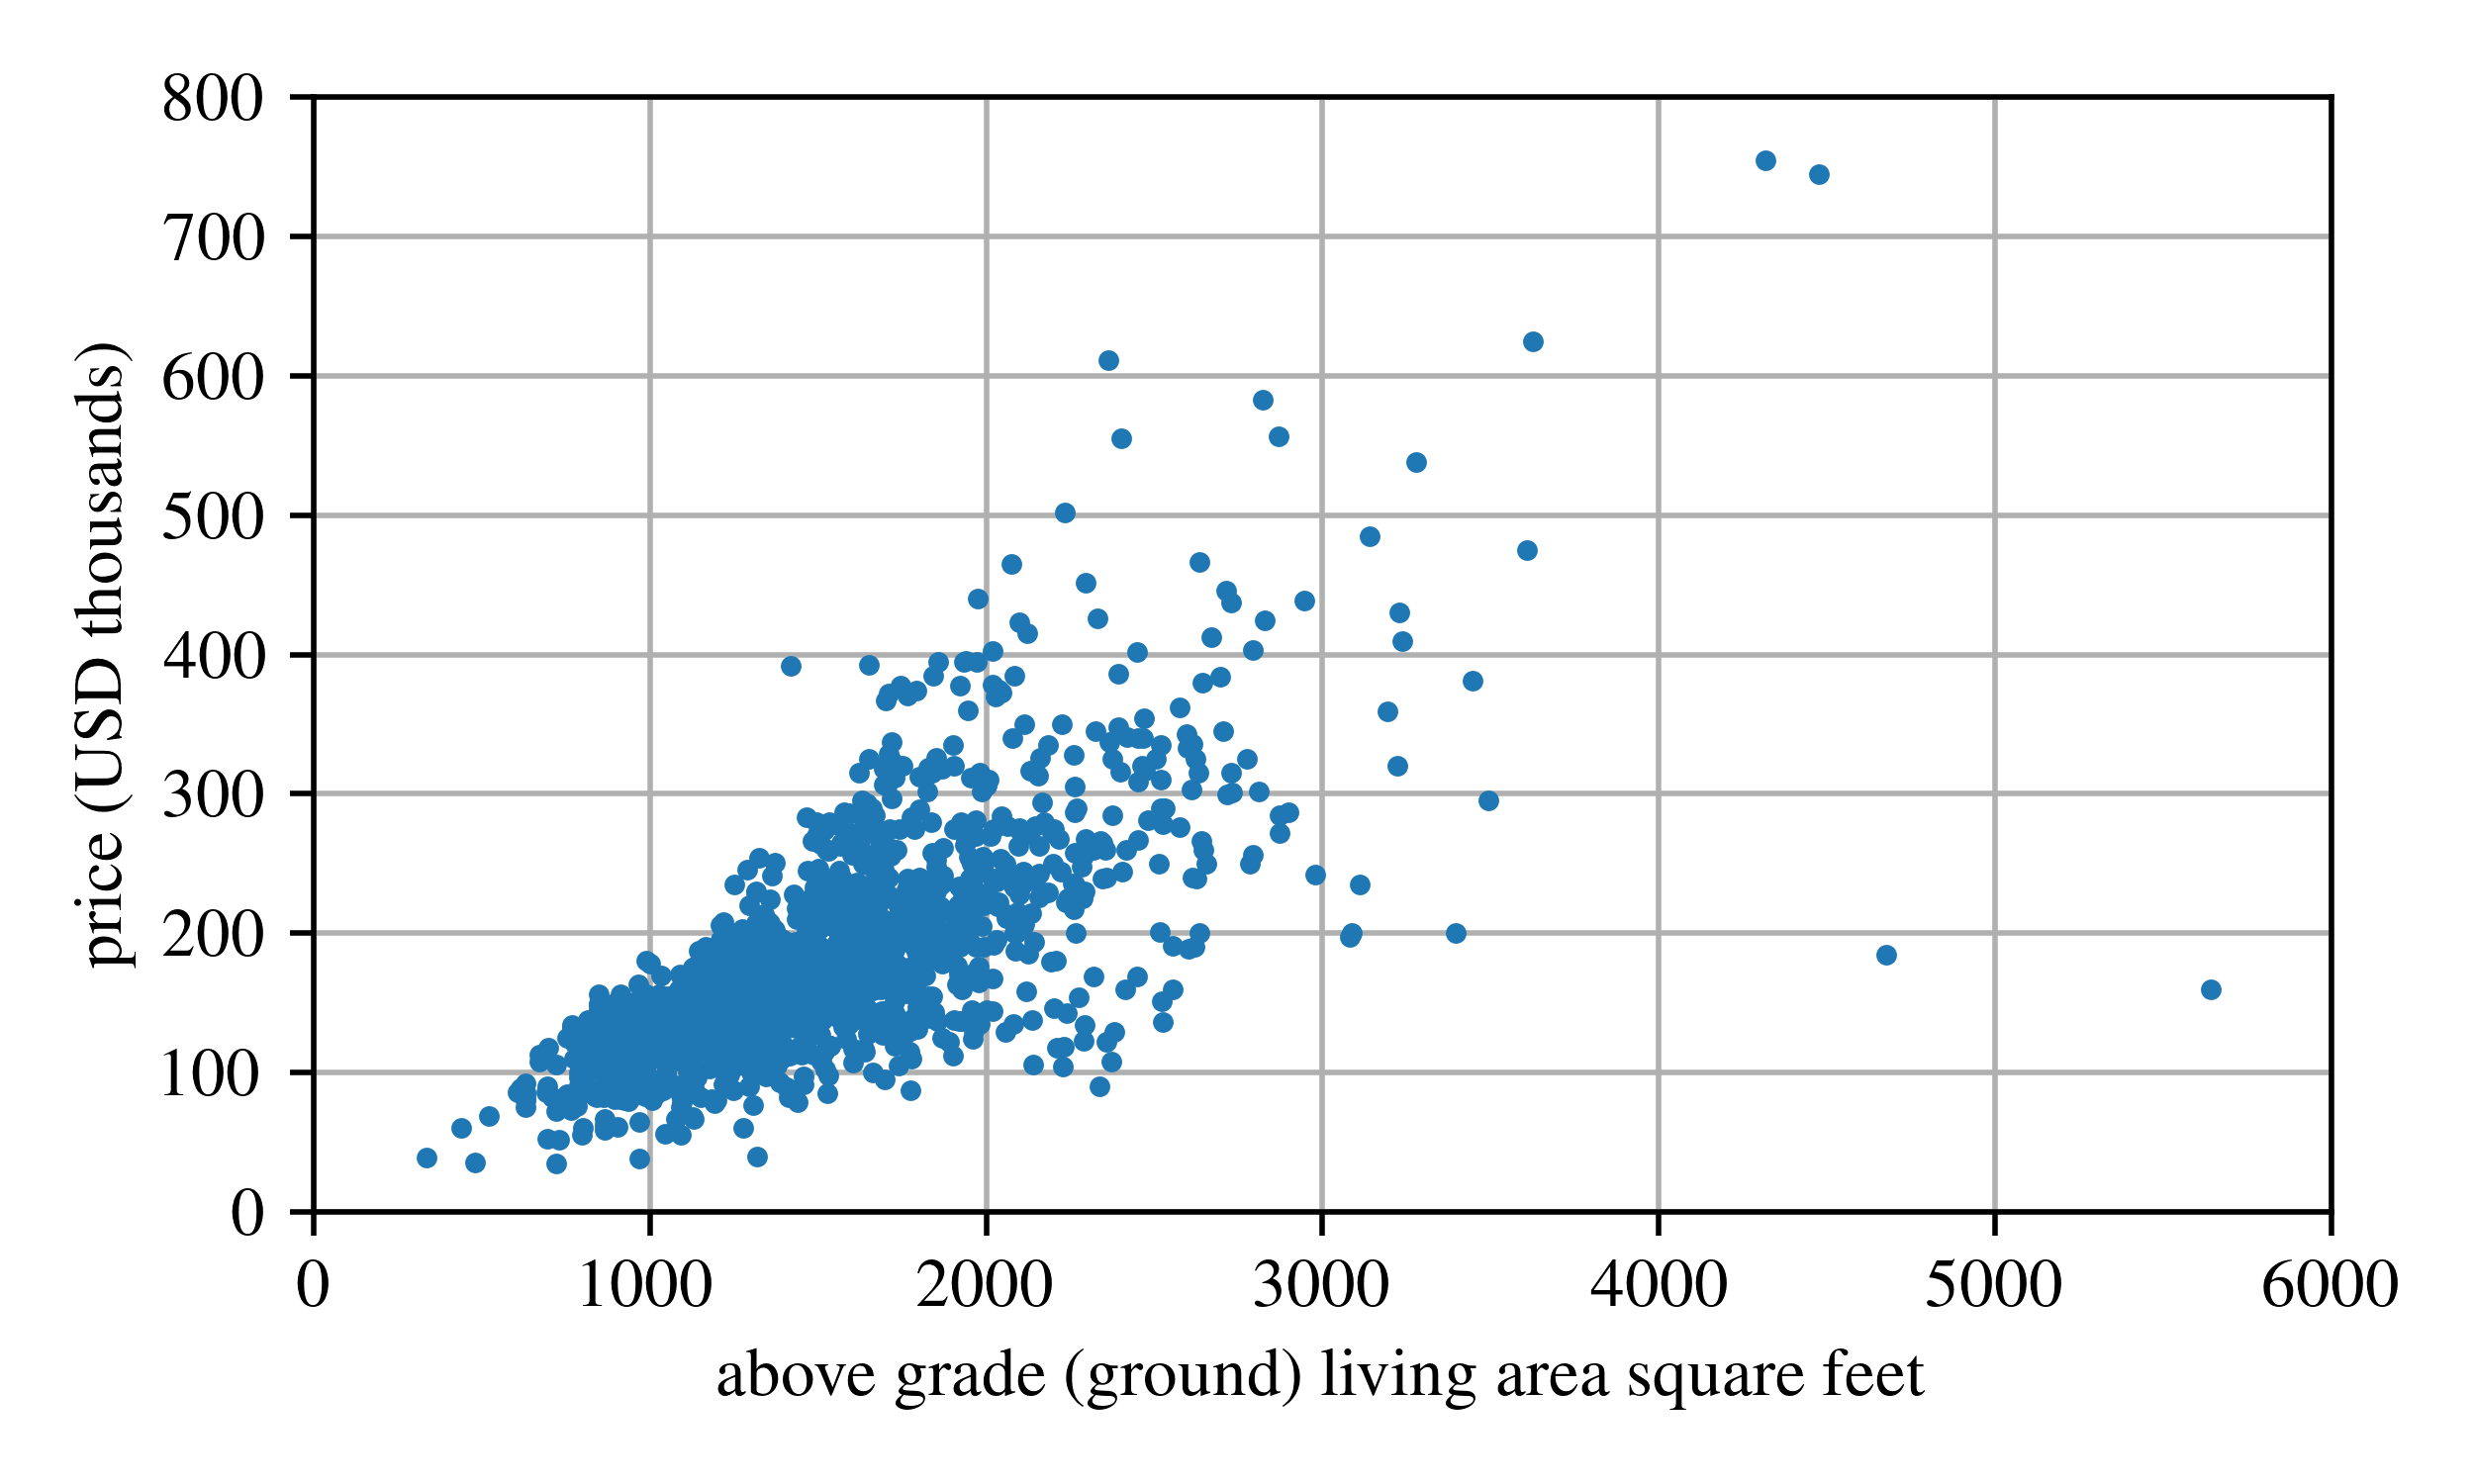
\includegraphics[]{../figures/Ames_simple_linear_regression_model_1.png}
    \caption{Ames housing data.}
    \label{fig:Ames_simple_linear_regression_model_1}
\end{figure}

A clear trend is observable, despite the data's noise (i.e., partial randomness): the value of a house increases with the above ground living area. Therefore, the house value can be modeled as a linear function of the above ground living area:
\begin{equation}
\text{price\_model} = \theta_1 + \theta_2 \times \text{above\_ground\_living\_area}
\end{equation}
This model comprises two parameters, $\theta_1$ and $\theta_2$, which can be adjusted to represent any linear relationship.

\begin{figure}[H]
    \centering
    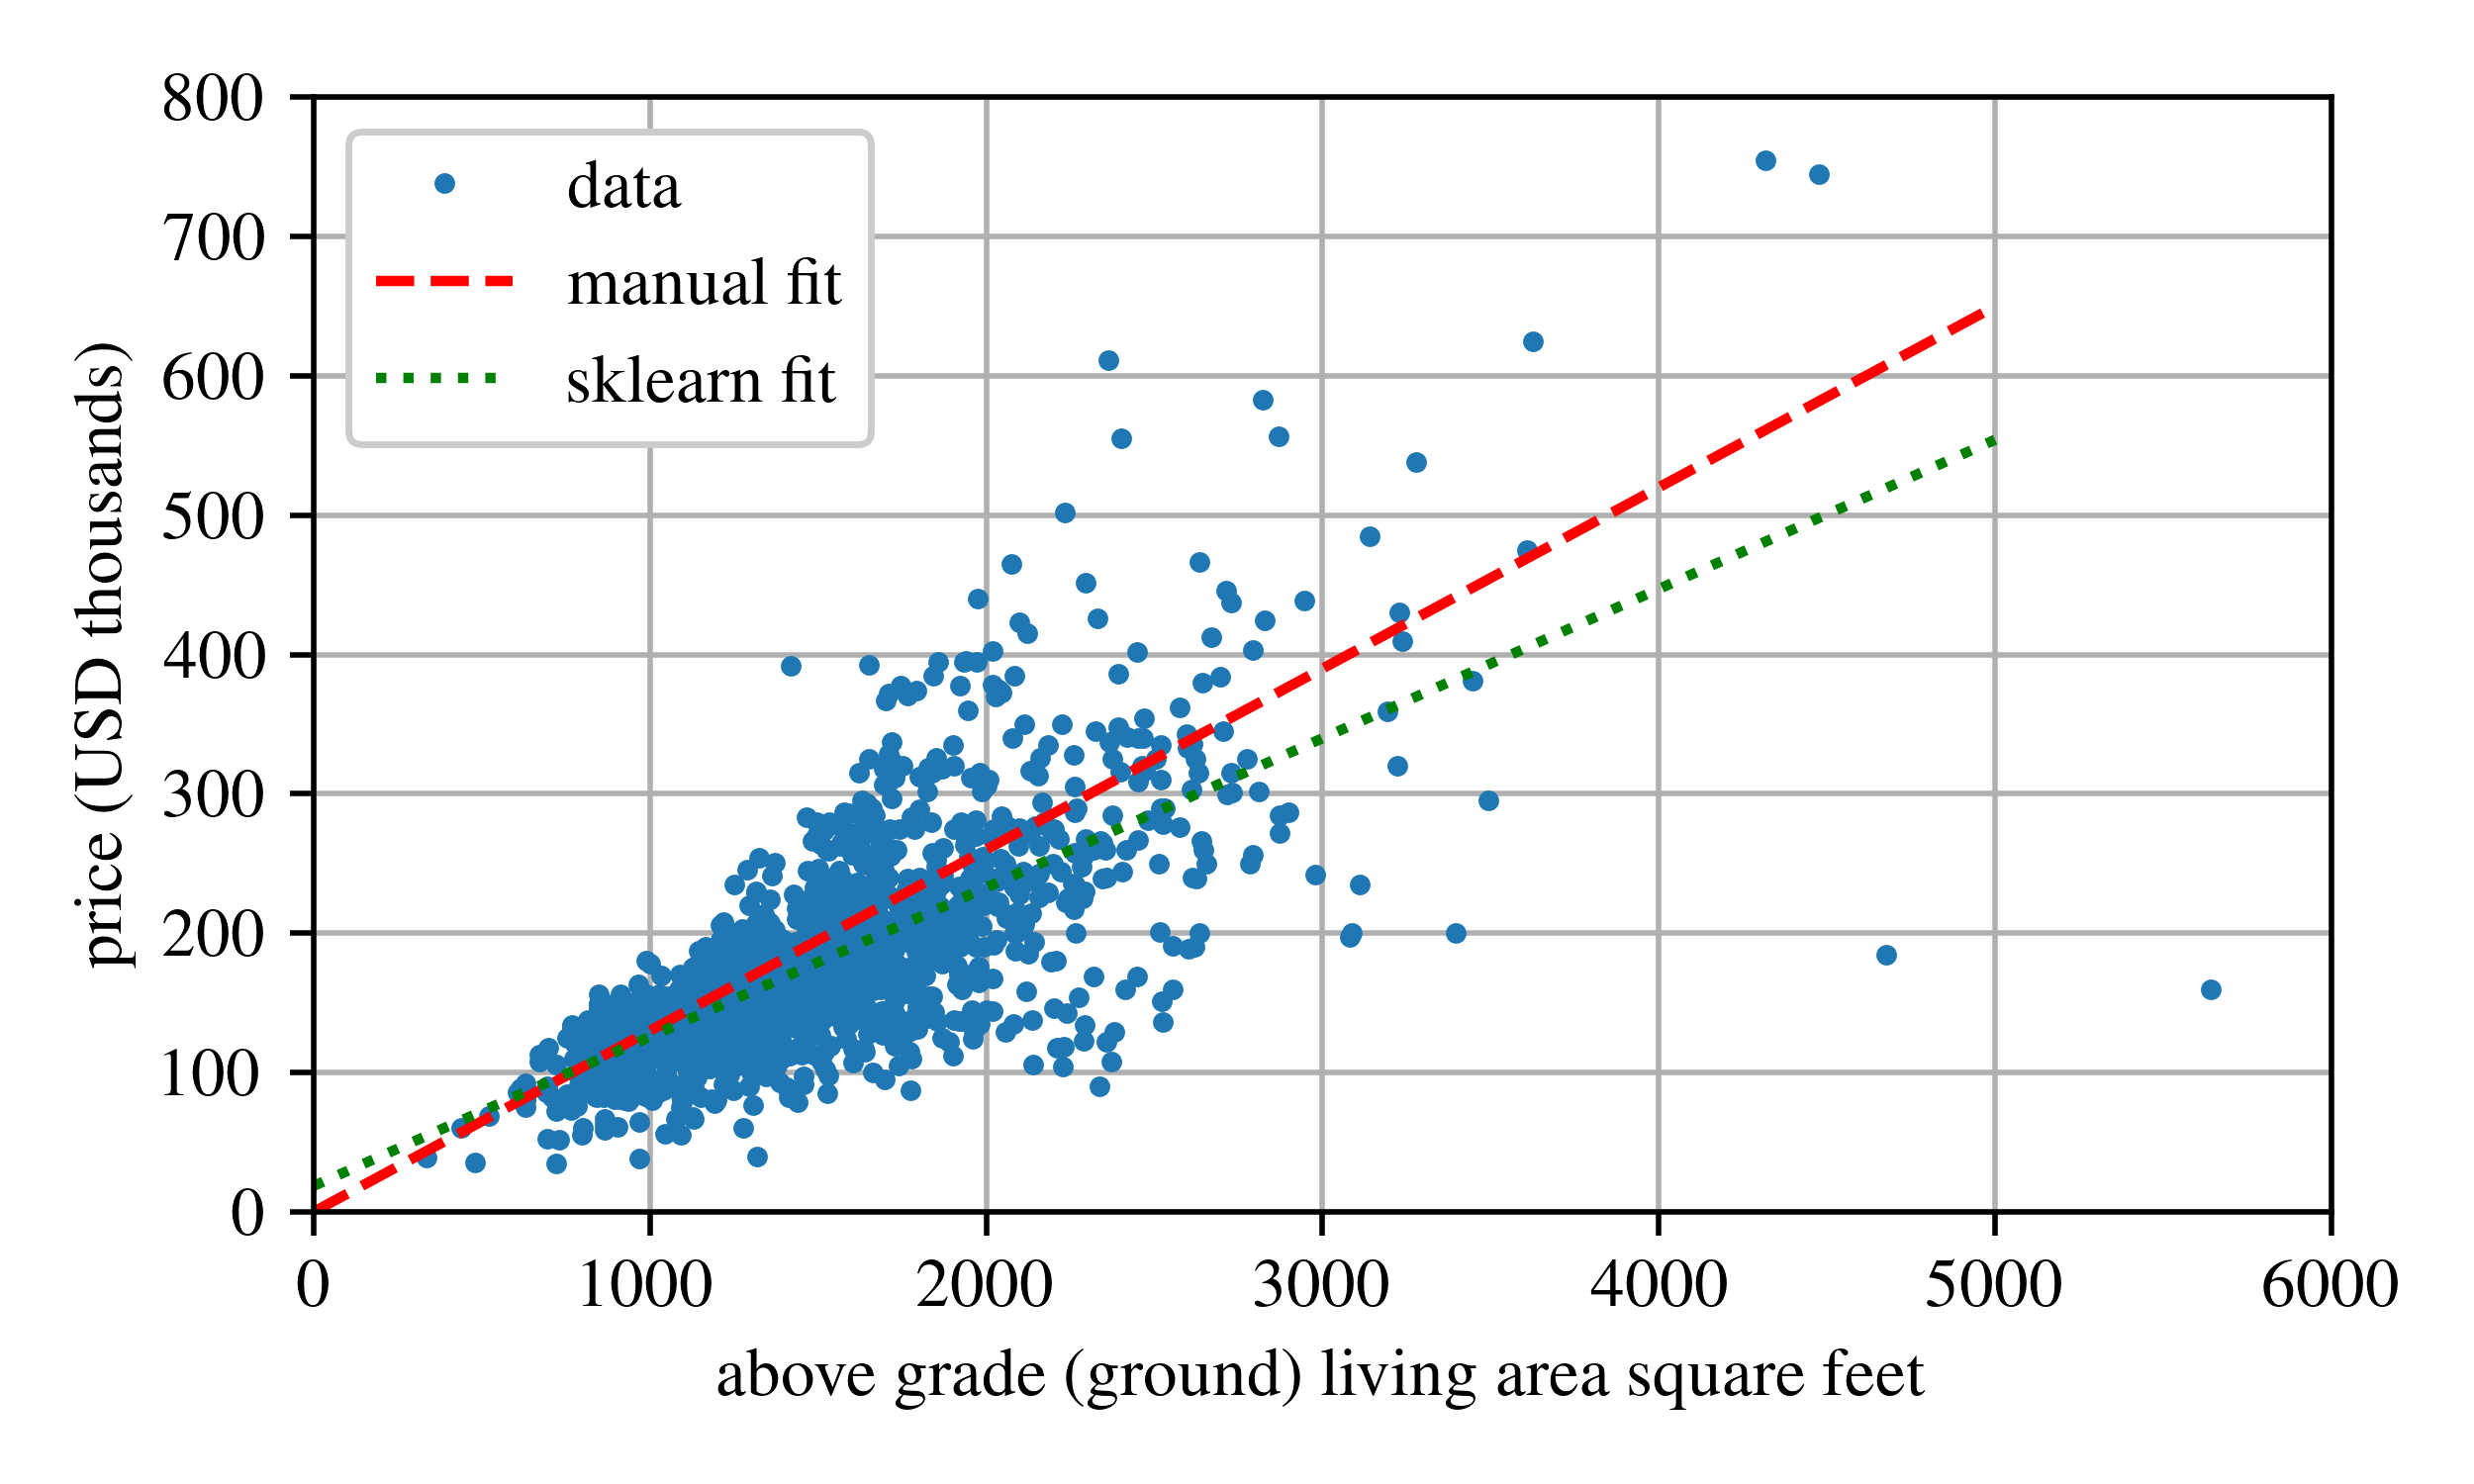
\includegraphics[]{../figures/Ames_simple_linear_regression_model_2.png}
    \caption{Ames housing data with trend lines.}
    \label{fig:GDP_data_trend}
\end{figure}








\begin{mdframed}[middlelinewidth=0.5mm]
\begin{center}
\gr{Notations}
\end{center}

\begin{itemize}
    \item $\textbf{x}$: a lowercase, bolded variable that denotes a vector.
    \item $\textbf{X}$: an uppercase, bolded variable that represents a matrix.
    \item $\textbf{X}$: this denotes the feature matrix, also known as the input matrix.
    \item $\textbf{y}$: this is the label vector corresponding to the feature matrix, representing the target outputs.
    \item $\textbf{x}^{(i)}$ represents the $i^\text{th}$ instance in the dataset $\textbf{X}$. For instance, a dataset about cats might include an entry for a specific cat named Mittens. This entry (labelled $y$) could detail several attributes such as age, weight, and length.
    \item $h$: the hypothesis or prediction function that, given a feature vector $\textbf{X}$, outputs the predicted values $\hat{\textbf{y}} = h(\textbf{X})$.
    \item $n$: the total number of features in the dataset, which defines the complexity or degree of the model.
    \item $m$: the total number of instances in the dataset.
    \item $\hat{x}$: an estimated value, indicated by a hat, and pronounced as ``$x$-hat''.
\end{itemize}
\end{mdframed}

\subsubsection{Closed Form Solution}

Before you can tune a model's parameters, you need a clear way to judge how well it fits the data. The standard approach is to define a cost function that assigns a numerical penalty to poor fits; lower values indicate better performance. For a linear model, this cost function measures the difference between the model's predictions and the actual training targets, and you minimize that difference using Ordinary Least Squares linear regression. Practically, you feed your training data into the algorithm, which then solves for the parameter values that align the linear relationship most closely to the data. In Python, this procedure is implemented in \texttt{scikit-learn} as \texttt{sklearn.linear\_model.LinearRegression}.

%
%To determine the optimal parameter values that enhance your model's performance, it is essential to define a suitable performance measure. 
%\begin{itemize}
%    \item We establish a cost function to quantify the inadequacy of the fit, where a lower value indicates a better fit.
%    \item For a linear model, we utilize a cost function that calculates the discrepancy between the model's predictions and the actual training data. The goal is to minimize this discrepancy, commonly addressed in Ordinary Least Squares Linear Regression.
%    \begin{itemize}
%        \item This involves inputting your training data into the algorithm, which then determines the parameters that best align the linear model with your data.
%        \item The function is implemented in scikit-learn as ``sklearn.linear\_model.LinearRegression''.
%    \end{itemize}
%\end{itemize}

In the context of the Ames housing data, a straightforward cost function used is the Mean Squared Error (MSE), defined as
\begin{equation}
\text{MSE} = J = \frac{1}{m} \sum_{i=1}^{m} (\hat{y}_i-y_i)^2
\end{equation}
\noindent where $m$ is the number of dataset instances, and $J$ serves as a general representation of the cost function in machine learning contexts.

The MSE is also applied to minimize the error in a linear regression model, with the hypothesis $h_\theta$, trained on dataset $\textbf{X}$. This is expressed as:
\begin{equation}
\text{MSE}(\textbf{X},h_\theta) = J = \frac{1}{m} \sum_{i=1}^{m} (\pmb{\theta}^\text{T}\textbf{x}^{(i)}-y^{(i)})^2
\end{equation}
\noindent where the objective is to minimize the cost function by iteratively refining the values of $\pmb{\theta}$.

\begin{figure}[H]
    \centering
    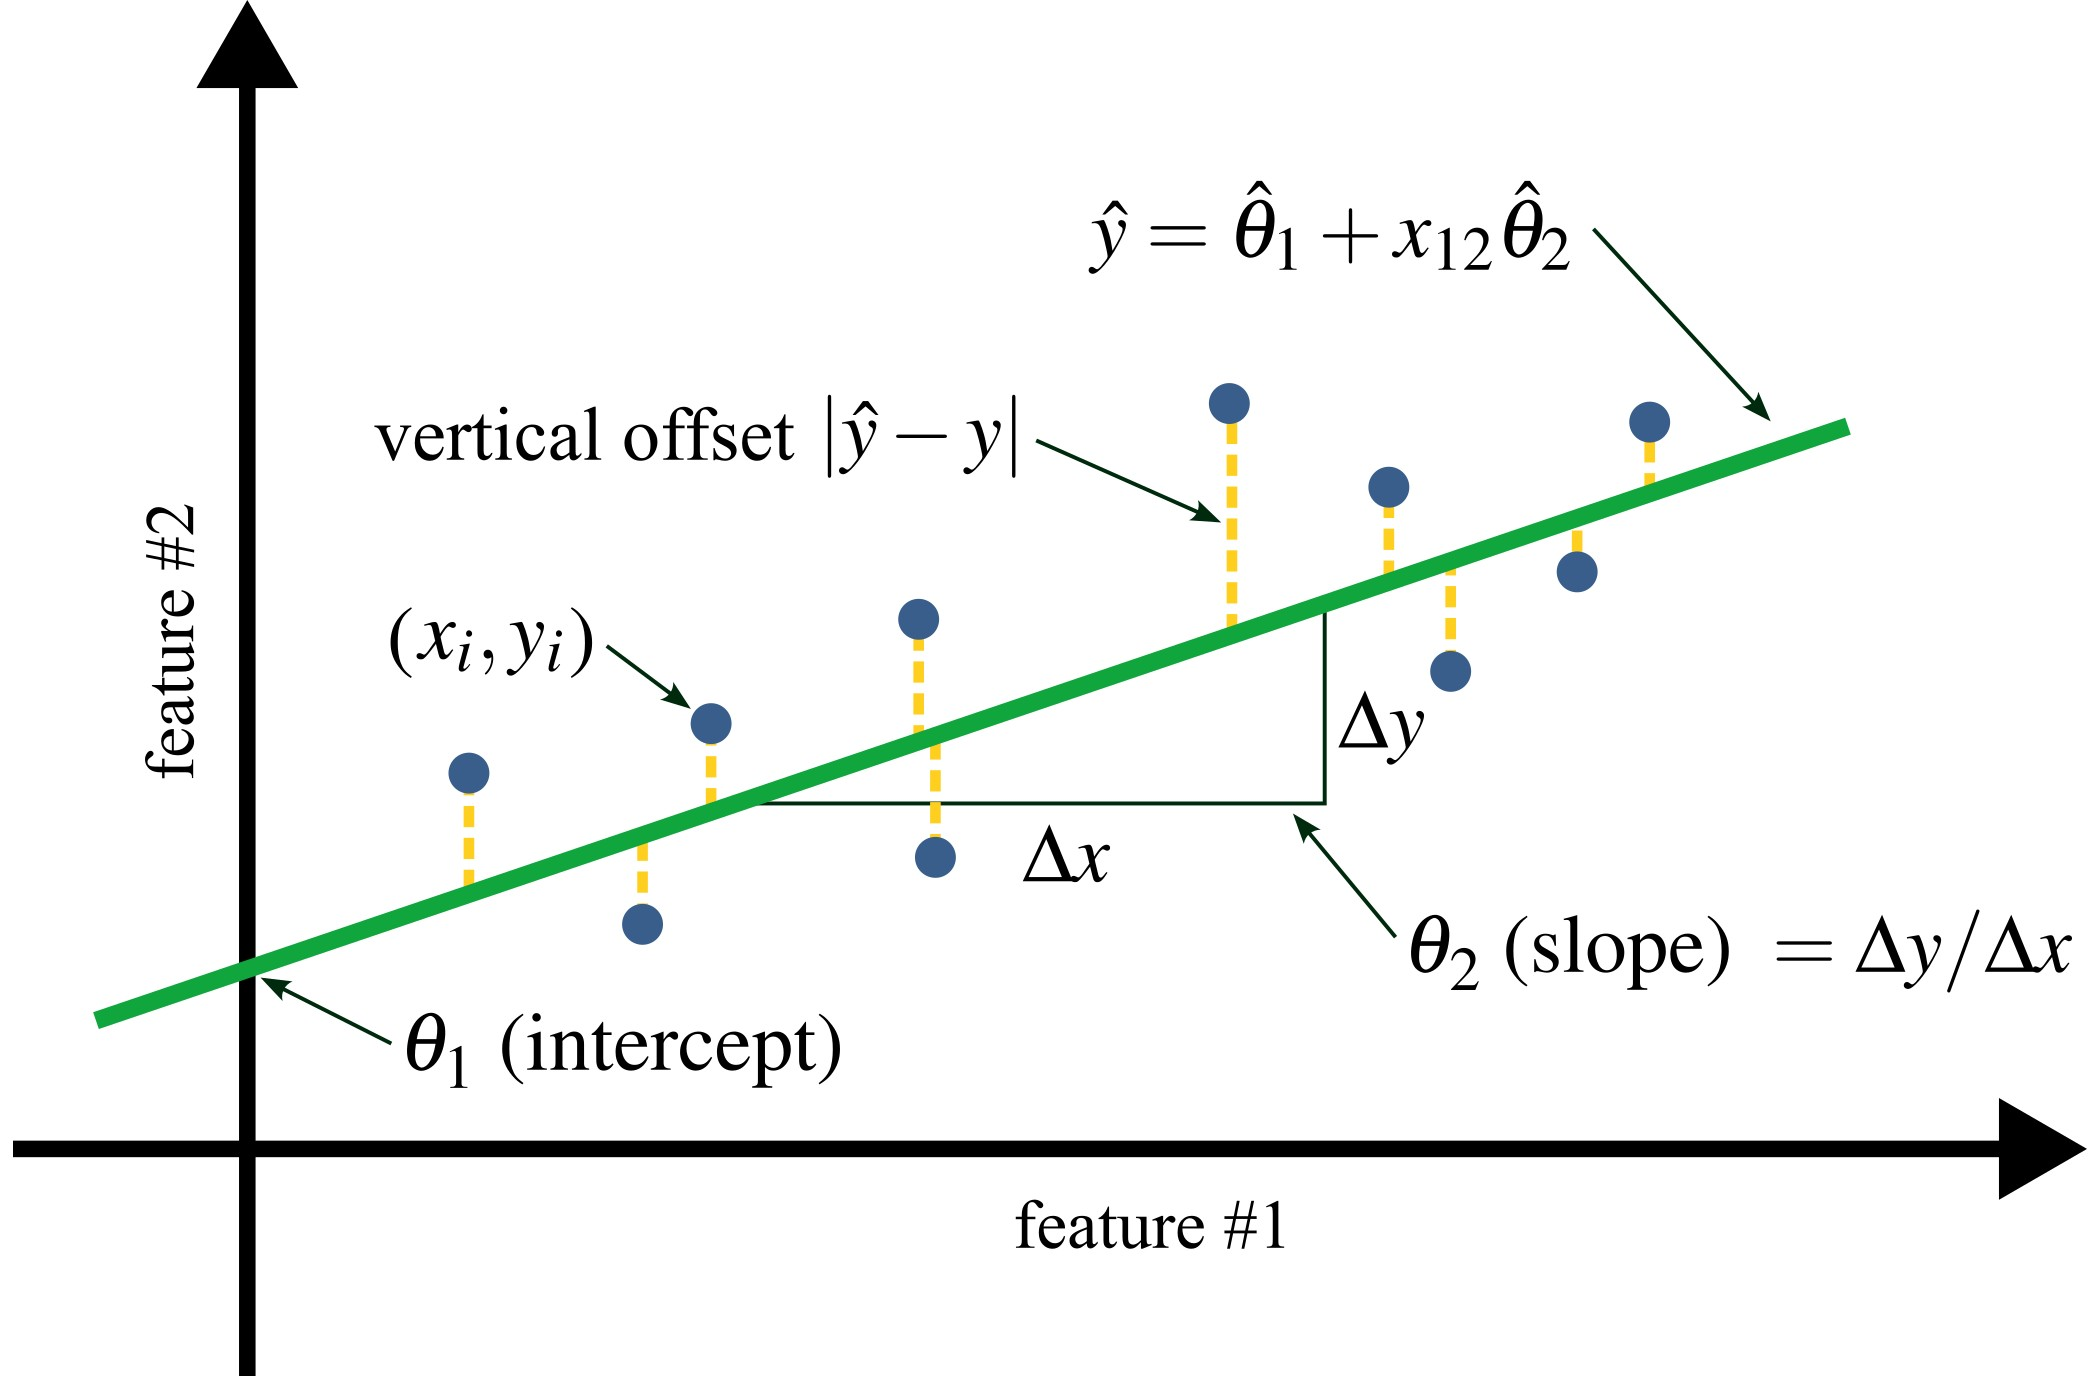
\includegraphics[width=4.2in]{../figures/least_squares}
    \caption{Linear regression of a two-feature dataset obtained with least squares.}
    \label{fig:least_squares}
\end{figure}

%% Math for the figure above
%$|\hat{y}-y|$ \\
%$x_i,y_i$ \\
%$\Delta x$ \\
%$\Delta y$ \\
%$\theta_1 \text{ (intercept)}$\\
%$\theta_2 \text{ (slope) } = \Delta y / \Delta x$ \\
%$\hat{y} = \hat{\theta}_1 + x_{12}\hat{\theta}_2$ \\


Consider a dataset containing $n$ observations, denoted as $(y_i, x_i)^n_{i=1}$. Each observation $i$ consists of a scalar response $y_i$ and a column vector $x_i$ that holds the values for $p$ predictors (regressors), represented as $x_{ij}$ where $j = 1, \dots, p$. In the context of a linear regression model, the response variable $y_i$ is modeled as a linear combination of the regressors, influenced by an error term $\epsilon_i$:
\begin{equation}
 y_i = \theta_1x_{i1}+\theta_2x_{i2}+\hdots+\theta_yx_{im}+\epsilon_i 
\end{equation}
This model can also be written in matrix notation as
\begin{equation}
\textbf{y} = \textbf{X} \pmb{\theta} + \epsilon
\end{equation}
Where: 
\begin{equation}
	\textbf{X} = \begin{bmatrix}
	x_{11} & x_{12} & \hdots & x_{1m} \\
	x_{21} & x_{22} & \hdots & x_{2m} \\
	\vdots & \vdots & \ddots & \vdots \\
	x_{n1} & x_{n2} & \hdots & x_{nm}
	\end{bmatrix},\;
	\pmb{\theta} = \begin{bmatrix}
	\theta_1 \\
	\theta_2 \\
	\vdots \\
	\theta_p
	\end{bmatrix},\;
	\textbf{y}=\begin{bmatrix}
	y_1 \\
	y_2 \\
	\vdots \\
	y_n
	\end{bmatrix}
\end{equation}
However, the best-fit model $\hat{y}$ will not be able to account for the unmodeled error, therefore: 
\begin{equation}
 \hat{y}_i = \hat{\theta}_1x_{i1}+\hat{\theta}_2x_{i2}+\hdots+\hat{\theta}_m x_{im}
\end{equation}
or 
\begin{equation}
 \hat{\textbf{y}} = \textbf{X} \hat{\pmb{\theta}}
\end{equation}


This goal is to find $\hat{\theta}$ such that the error is minimized. Mathmatically, this is simple enough as the $\hat{\theta}$ Is the minimization of the lease-squares hyperplane, or:
\begin{equation}
\hat{\pmb{\theta}}=(\textbf{X}\textsuperscript{T}\textbf{X})^{-1}\textbf{X}\textsuperscript{T}\textbf{y}
\label{eq:normal_equation}
\end{equation}
Equation~\ref{eq:normal_equation} is referred to as the normal equation. Consider a simple linear model with $p = 2$, where $x_{11} = 1$. In this scenario, $x_{11}$ acts as the bias term of the equation, whereas the remaining elements of $\textbf{X}$ represent the data. Without this bias term, the solution would only address the slope of the line. Subsequently, solving for $\hat{\theta}_1$ and $\hat{\theta}_2$ yields:
\begin{equation}
 [x_{11}x_{12}][\hat{\theta}_1\hat{\theta}_2] = \hat{y}
\end{equation}
As $x_{11} = 1$ (again, called the bias term) this becomes:
\begin{equation}
 \hat{y} = \hat{\theta}_1 + x_{12}\hat{\theta}_2
\end{equation}
This is simply another expression for the equation of a liner line:
\begin{equation}
y = mx + b
\end{equation}
Solving the model output for a input or a series of inputs can than be done simply enough. 

\begin{figure}[H]
	\centering
	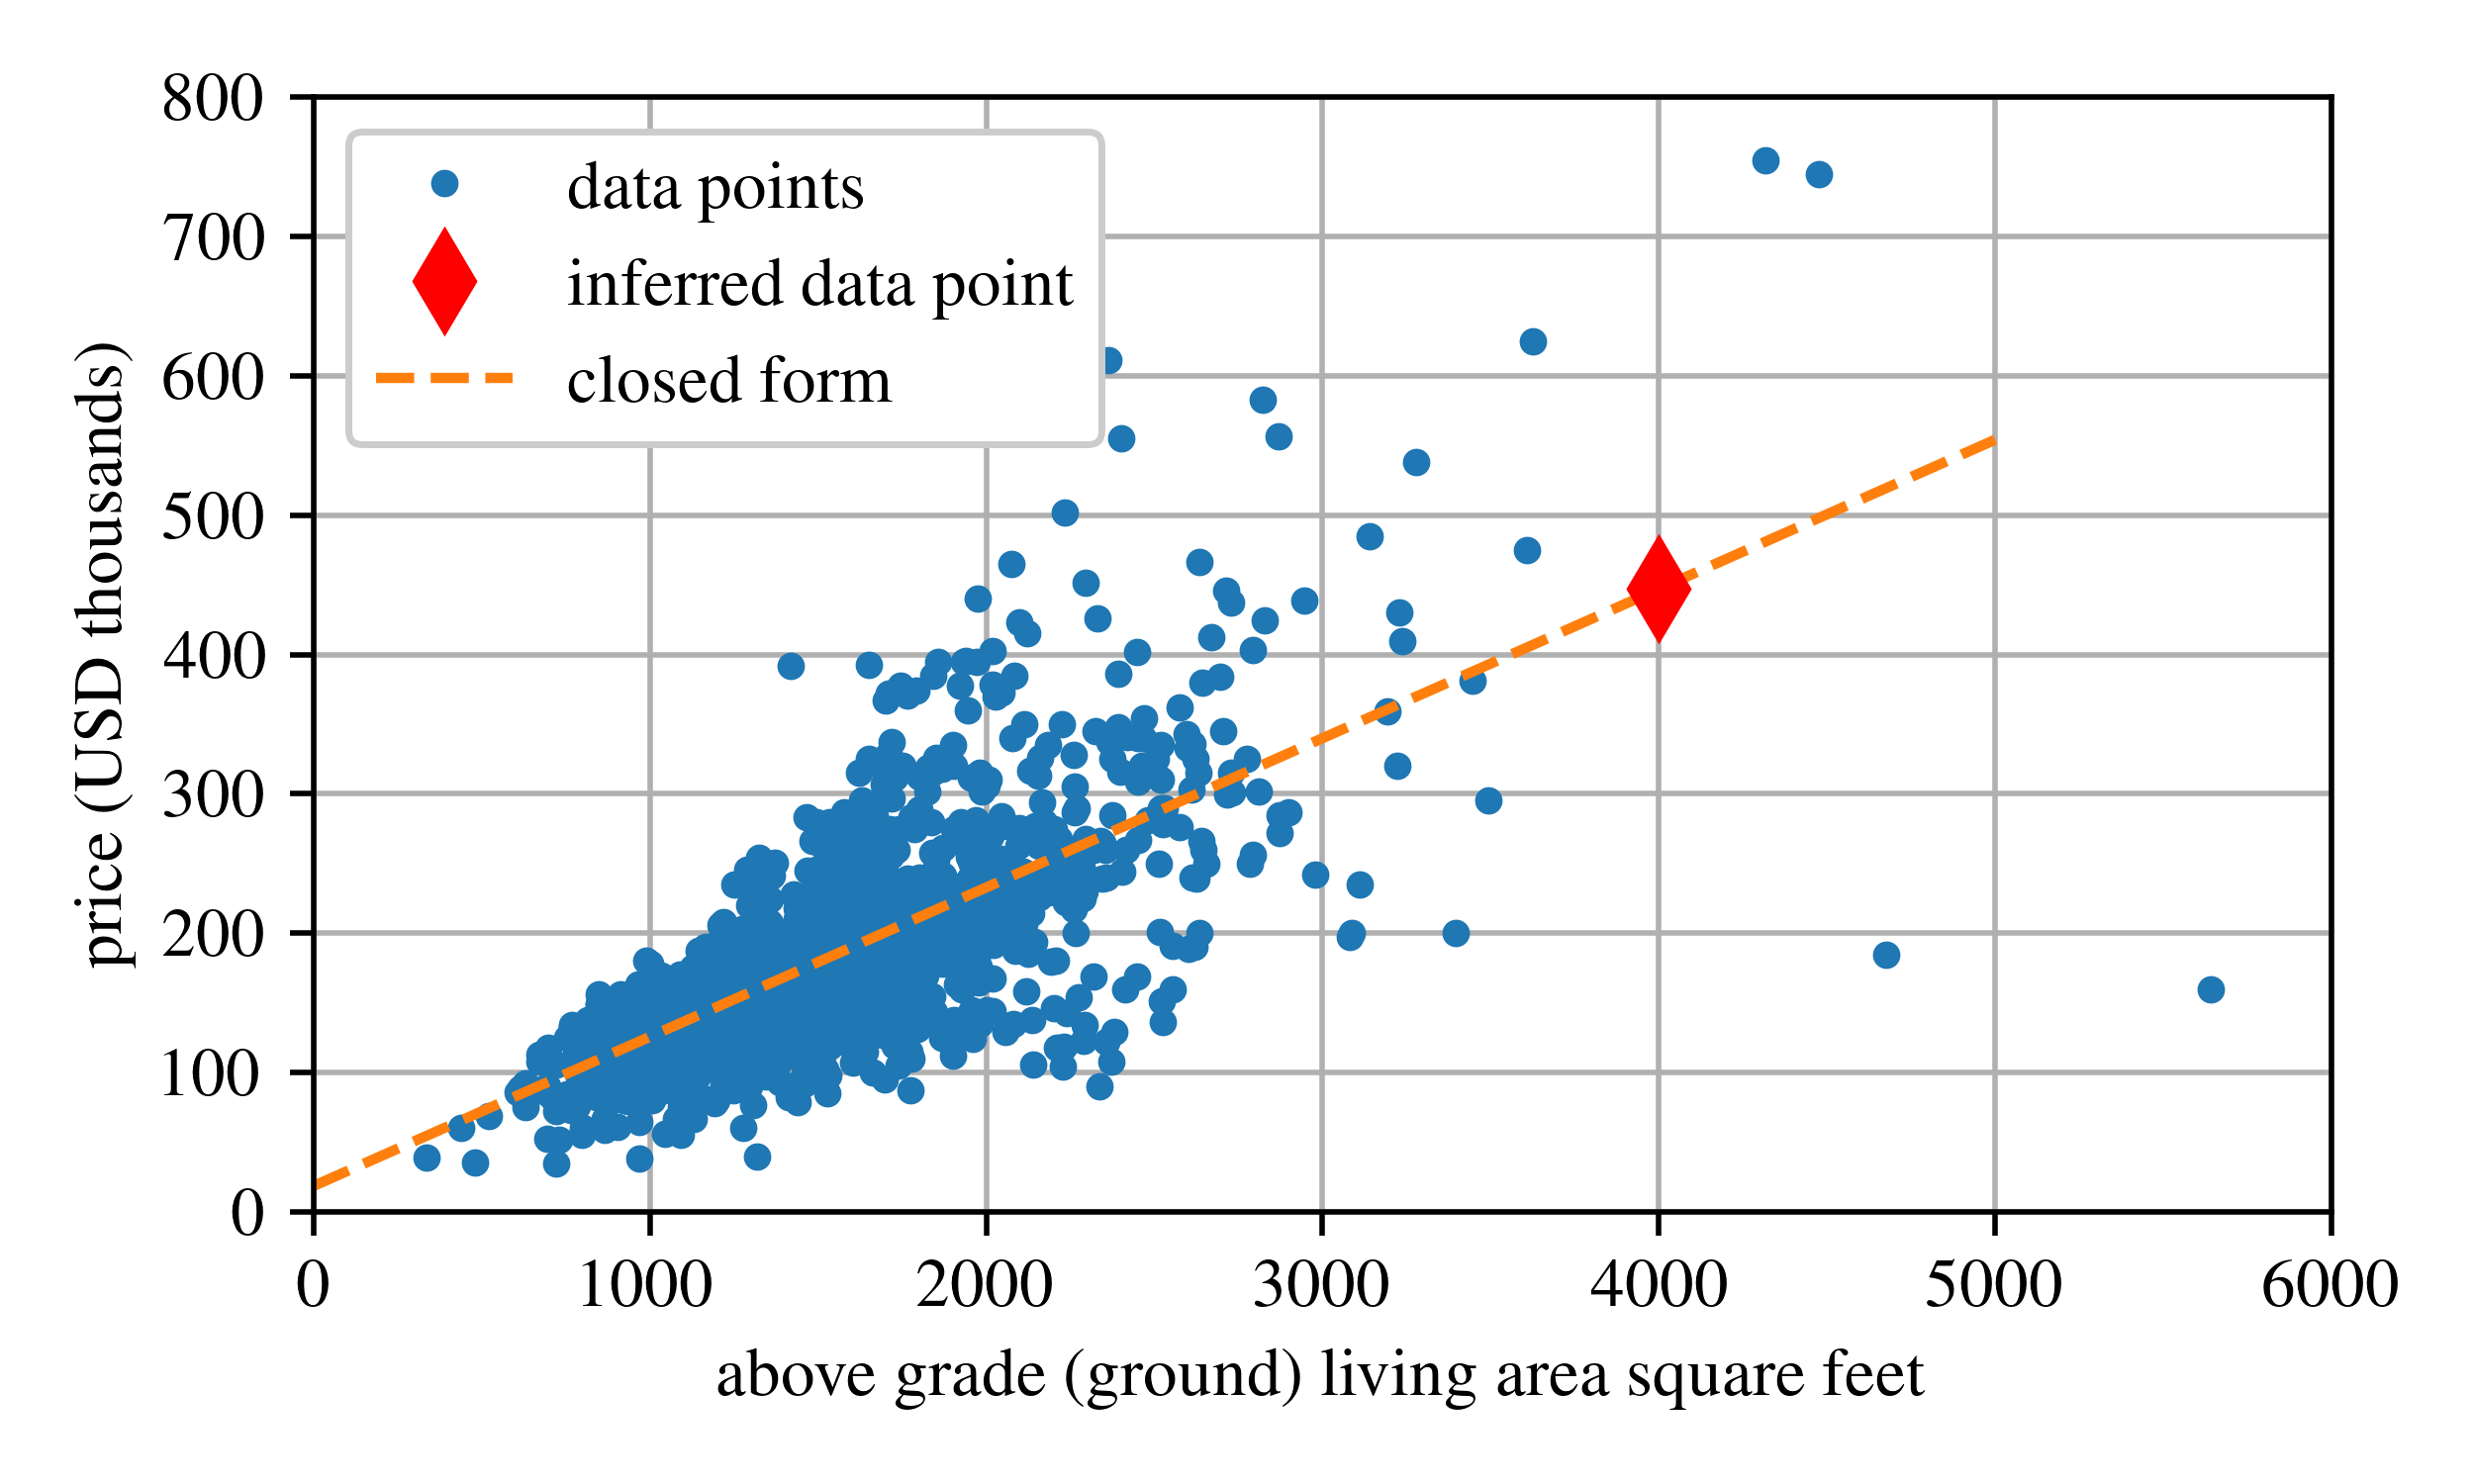
\includegraphics[]{../figures/Ames_simple_linear_regression_model_3.png}
	\caption{Ames housing data inferred.}
	\label{fig:Ames_simple_linear_regression_model_3}
\end{figure}


\subsubsection{Computational Complexity}

The Normal Equation calculates the inverse of $\textbf{X}^\text{T}\textbf{X}$, an $n \times n$ matrix, where $n$ represents the number of features. The computational complexity of matrix inversion generally ranges from $O(n^{2.4})$ to $O(n^3)$, depending on the specific algorithm used. Consequently, doubling the number of features would increase the computational effort by approximately $2^{2.4} \approx 5.3$ to $2^3 = 8$ times.


\begin{mdframed}[middlelinewidth=0.5mm]
\begin{center}
\rd{WARNING}
\end{center}
When the number of features becomes very large, for example around $100,000$, solving the Normal Equation becomes extremely slow.
\end{mdframed}



On the positive side, the computational complexity of this equation is linear with respect to the number of instances in the training set, denoted as $O(m)$. This allows it to efficiently handle large training sets, as long as they fit within memory.

Furthermore, once your Linear Regression model is trained (whether through the Normal Equation or another method), making predictions is very quick. The computational effort is linear in relation to both the number of instances you wish to predict and the number of features. Essentially, predicting for twice as many instances or features will approximately double the computation time.

Next, we will explore different methods for training a Linear Regression model that are more appropriate for scenarios with a large number of features, or when the training data exceeds memory capacity.

\begin{example}
\textbf{Linear Regression - Ames Housing Dataset}

\noindent This example uses the Ames housing dataset to model the relationship between above-ground living area and house price using linear regression. It compares a manual fit, a closed-form solution, and gradient descent, alongside Scikit-Learn's \texttt{LinearRegression} and \texttt{SGDRegressor}, to illustrate how each method fits a line to the data.

\end{example}

%\lstset{%
%caption={Example functions for Python code.},
%label={lst:functions},
%language=Python,
%basicstyle=\ttm,
%morekeywords={self},              % Add keywords here
%keywordstyle=\ttb\color{deepblue},
%emph={MyClass,__init__},          % Custom highlighting
%emphstyle=\ttb\color{deepred},    % Custom highlighting style
%stringstyle=\color{deepgreen},
%frame=tb,                         % Any extra options here
%showstringspaces=false
%}
%\begin{lstlisting}
%i=20
%
%class MyClass(Yourclass):
%    def __init__(self, my, yours):
%        bla = '5 1 2 3 4'
%        print bla
%
%# this is a comment
%for i in range(10):
%	i=10
%
%
%
%\end{lstlisting}


Gradient Descent is a versatile optimization algorithm capable of finding optimal solutions across a broad spectrum of problems. The core concept of Gradient Descent involves iteratively adjusting parameters to minimize a cost function \protect\footnotemark[1]. Consider the analogy of being lost in a dense fog in the mountains and seeking to descend:
\begin{enumerate}
\item You sense the ground's slope under your feet (the local gradient).
\item You descend in the direction of the steepest descent.
\item Reaching a point where the local gradient is zero indicates that you have found a minimum.
\end{enumerate}
	
\footnotetext[1]{Ruder, Sebastian. ``An overview of gradient descent optimization algorithms.'' arXiv preprint arXiv:1609.04747 (2016).}


The Gradient Descent process starts with random initialization of the parameter $\theta$, followed by gradual improvements. Each incremental step aims to reduce the cost function until the algorithm converges to a minimum.

\begin{figure}[H]
    \centering
    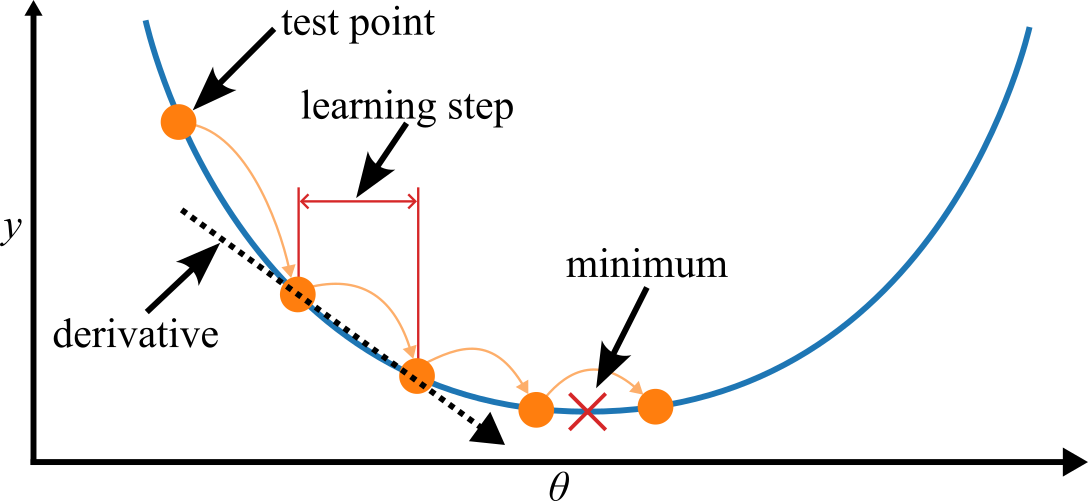
\includegraphics[]{../figures/gradient_descent_1}
    \caption{Illustration of gradient descent.}
    \label{fig:gradient_descent_1}
\end{figure}

A critical aspect of Gradient Descent is the step size, controlled by the learning rate hyperparameter. A small learning rate leads to a slow convergence, requiring many iterations. Conversely, a high learning rate might cause the algorithm to overshoot the minimum, potentially causing divergence and failing to find an optimal solution.

\begin{figure}[H]
    \centering
    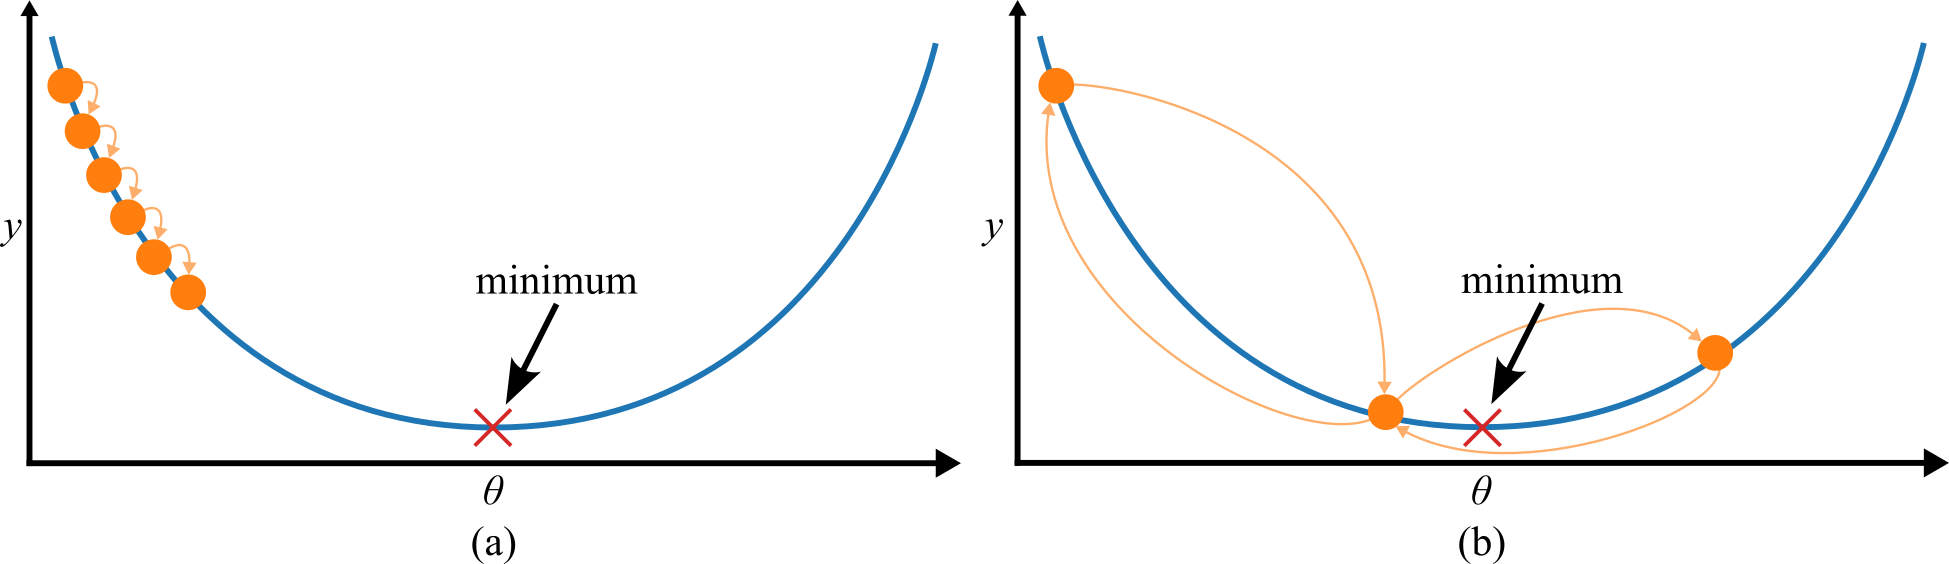
\includegraphics[]{../figures/gradient_descent_2}
    \caption{Effect of learning rate in gradient descent, showing: (a) a slow search with a low step size, and (b) a search with a large step size that oscillates around the minimum without ever finding the minimum.}
    \label{fig:gradient_descent_2}
\end{figure}



Cost functions do not always present themselves as neat, concave shapes. They can feature obstacles such as holes, ridges, plateaus, and various complex topographies that complicate the convergence to the minimum. The challenges associated with Gradient Descent include:
\begin{itemize}
\item Starting the algorithm from a random point on the left may lead to convergence at a local minimum rather than the more optimal global minimum.
\item Initiating on the right might result in a prolonged journey across a plateau, and terminating the process too soon could prevent reaching the global minimum.
\end{itemize}

\begin{figure}[H]
    \centering
    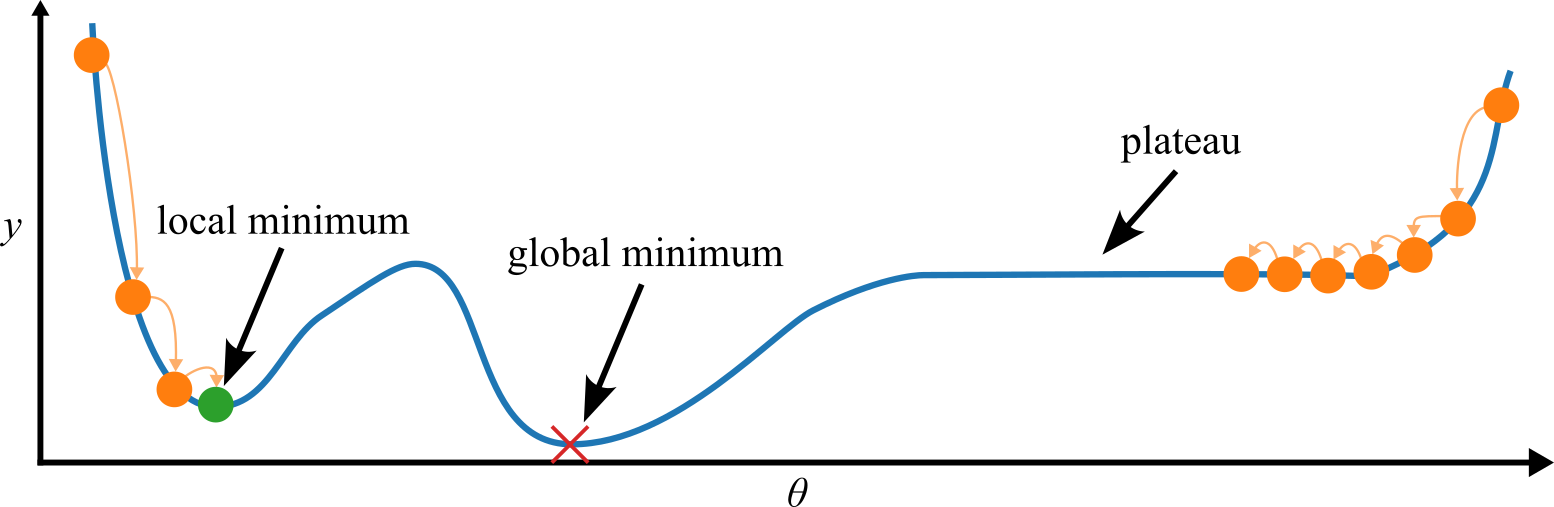
\includegraphics[]{../figures/gradient_descent_3}
    \caption{Gradient features and descent challenges.}
    \label{fig:gradient_descent_3}
\end{figure}

Fortunately, the Mean Squared Error (MSE) cost function for Linear Regression models is convex. This characteristic ensures that for any two points on the curve, the line segment joining them does not intersect the curve itself. Consequently:
\begin{itemize}
\item There are no local minima, only one global minimum exists.
\item It is a continuous function, and its slope changes smoothly.
\end{itemize}

These properties significantly benefit the optimization process: Gradient Descent can reliably approximate the global minimum given sufficient time and an appropriate learning rate.






\subsubsection{Comparison of Gradient Descent Methods}

Before looking into the mathematical details, let us examine how various gradient descent methods achieve the optimal solution, as illustrated in Figure~\ref{fig:Comparing_gradient_descent_methods}. Additionally, Table~\ref{table:Comparison_linear_regression} provides a comparative analysis of different gradient descent methods, highlighting their respective strengths and weaknesses.


\begin{figure}[H]
	\centering
	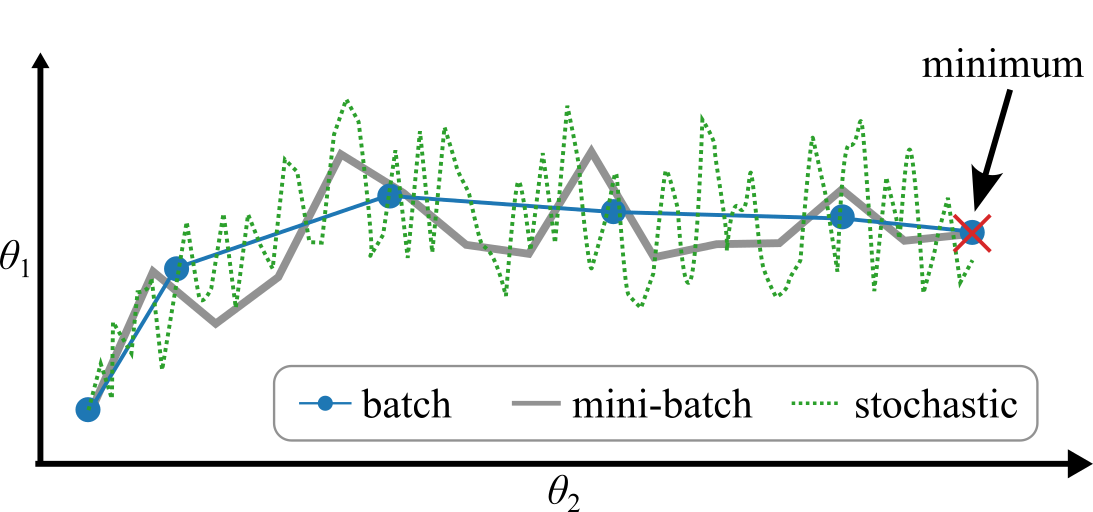
\includegraphics[]{../figures/comparing_gradient_descent_methods}
	\caption{Comparing gradient descent methods.}
	\label{fig:Comparing_gradient_descent_methods}
\end{figure}



% Please add the following required packages to your document preamble:
% \usepackage{booktabs}
\begin{table}[H]
\caption{Comparison of various linear regression solutions.}
\label{table:Comparison_linear_regression}
\resizebox{\textwidth}{!}{\begin{tabular}{@{}lllllll@{}}
\toprule
\multicolumn{1}{c}{algorithm} & {\begin{tabular}[c]{@{}c@{}}large number of\\  instances ($m$) \end{tabular}} & \multicolumn{1}{c}{\begin{tabular}[c]{@{}c@{}}data must\\ fit in memory\end{tabular}} & {\begin{tabular}[c]{@{}c@{}}large number of\\  features ($n$) \end{tabular}} & \multicolumn{1}{c}{hyperparams} & \multicolumn{1}{c}{\begin{tabular}[c]{@{}c@{}}scaling\\ required\end{tabular}} & \multicolumn{1}{c}{Scikit-Learn} \\ \midrule
normal equation & fast & yes & slow & 0 & no & \texttt{LinearRegression} \\
batch GD & slow & yes & fast & 2 & yes & n/a \\
stochastic GD & fast & no & fast &  $\ge 2$ & yes & \texttt{SGDRegressor} \\
mini-batch GD & fast & no & fast &  $\ge 2$ & yes & n/a \\ \bottomrule
\end{tabular}}
\end{table}




\begin{mdframed}[middlelinewidth=0.5mm]
\begin{center}
\bl{NOTE}
\end{center}
After training, there is minimal difference between the models: these algorithms converge on similar solutions and make predictions in a nearly identical manner.
\end{mdframed}






\subsubsection{Batch Gradient Descent}

\begin{figure}[H]
	\centering
	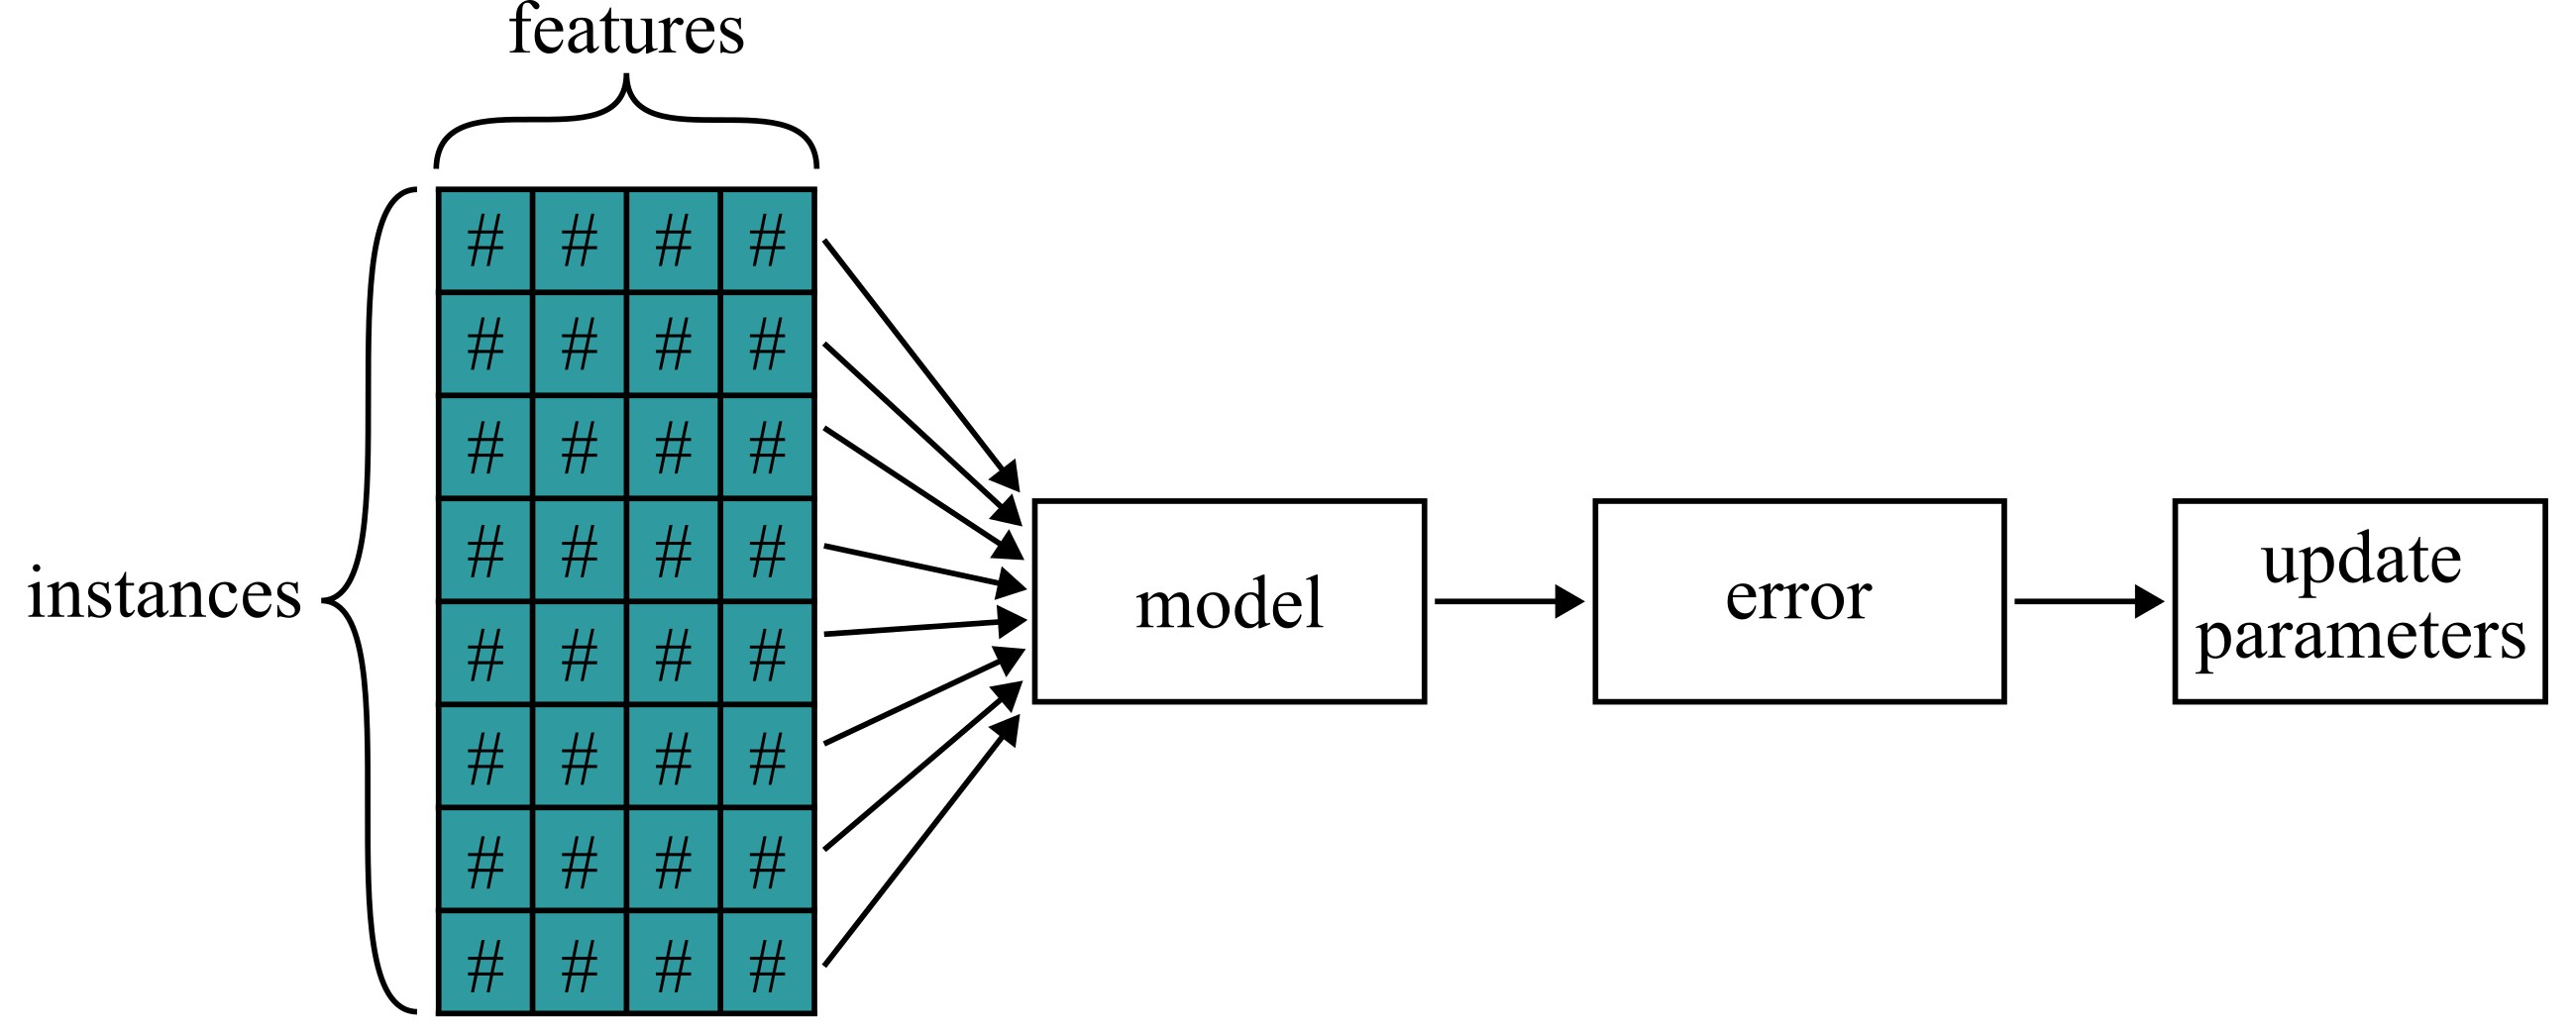
\includegraphics[width=5.4in]{../figures/gradient_descent_batch}
	\caption{Flowchart of Batch Gradient Descent.}
	\label{fig:gradient_descent_batch}
\end{figure}




Batch Gradient Descent processes the entire batch of training data $\textbf{X}$ at every step, which is the origin of its name, ``batch.'' Consider again our Mean Squared Error (MSE) cost function:
\begin{equation}
J = \frac{1}{m} \sum_{i=1}^{m} (\hat{y}_i - y_i)^2
\end{equation}
For a hypothesis $h_\theta$, the MSE for the dataset $\textbf{X}$ can be computed for each instance $\textbf{x}^{(i)}$ as follows:
\begin{equation}
J(\textbf{X}, h_\theta) = J = \frac{1}{m} \sum_{i=1}^{m} (\pmb{\theta}^\text{T}\textbf{x}^{(i)} - y^{(i)})^2
\end{equation}
With this foundation, we can implement gradient descent by computing the gradient of the cost function with respect to each parameter $\theta_j$. Specifically, this involves calculating how much the cost function changes when $\theta_j$ is altered slightly. This calculation is known as a partial derivative. Conceptually, it is akin to determining ``the slope of the mountain under my feet if I face east,'' then repeating the question facing north, and similarly for any other direction in a higher-dimensional space. The partial derivative of the cost function with respect to parameter $\theta_j$ is computed as:
\begin{equation}
\frac{\partial}{\partial \theta_j} J(\theta) = \frac{2}{m} \sum_{i=1}^{m}(\pmb{\theta}^\text{T}\textbf{x}^{(i)} - y^{(i)}) x_j^{(i)}
\label{eq:pd_cost_function}
\end{equation}



Rather than computing each partial derivative individually, all partial derivatives can be calculated simultaneously using the gradient vector, $\nabla_\theta J(\pmb{\theta})$, which encompasses all partial derivatives of the cost function for each model parameter:
\begin{equation}
	\nabla_\theta J(\pmb{\theta}) = \begin{pmatrix}
	\frac{\partial}{\partial \theta_0} J(\theta) \\
	\frac{\partial}{\partial \theta_1} J(\theta) \\
	\vdots  \\
	\frac{\partial}{\partial \theta_n} J(\theta)
	\end{pmatrix}
	= \frac{2}{m} \textbf{X}^\text{T} \cdot (\textbf{X} \pmb{\theta} - \textbf{y})
\end{equation}

\begin{mdframed}[middlelinewidth=0.5mm]
\begin{center}
\rd{WARNING}
\end{center}
Be aware that this method computes using the entire training set $\textbf{X}$ at every step of Gradient Descent, which is why the approach is named Batch Gradient Descent. Although this method can be exceedingly slow with large training sets, it performs well with numerous features, outpacing the Normal Equation in training Linear Regression models with extensive features.
\end{mdframed}

Once you obtain the gradient vector, which indicates the direction of ascent, the next step involves moving in the opposite direction, effectively going downhill. This is achieved by subtracting $\nabla_\theta J(\theta)$ from $\pmb{\theta}$, incorporating the learning rate $\eta$ to scale the step size:
\begin{equation}
\pmb{\theta}^{(\text{next step})} = \pmb{\theta} - \eta \nabla_\theta J(\pmb{\theta})
\end{equation}

Interestingly, this process aligns perfectly with the results from the Normal Equation. However, variations in the learning rate $\eta$ can significantly influence the outcomes. Figure~\ref{fig:learning_rates} illustrates the first 10 steps of Gradient Descent with three different learning rates, with the dashed line marking the starting point.




		\begin{figure}[H]
			\centering
			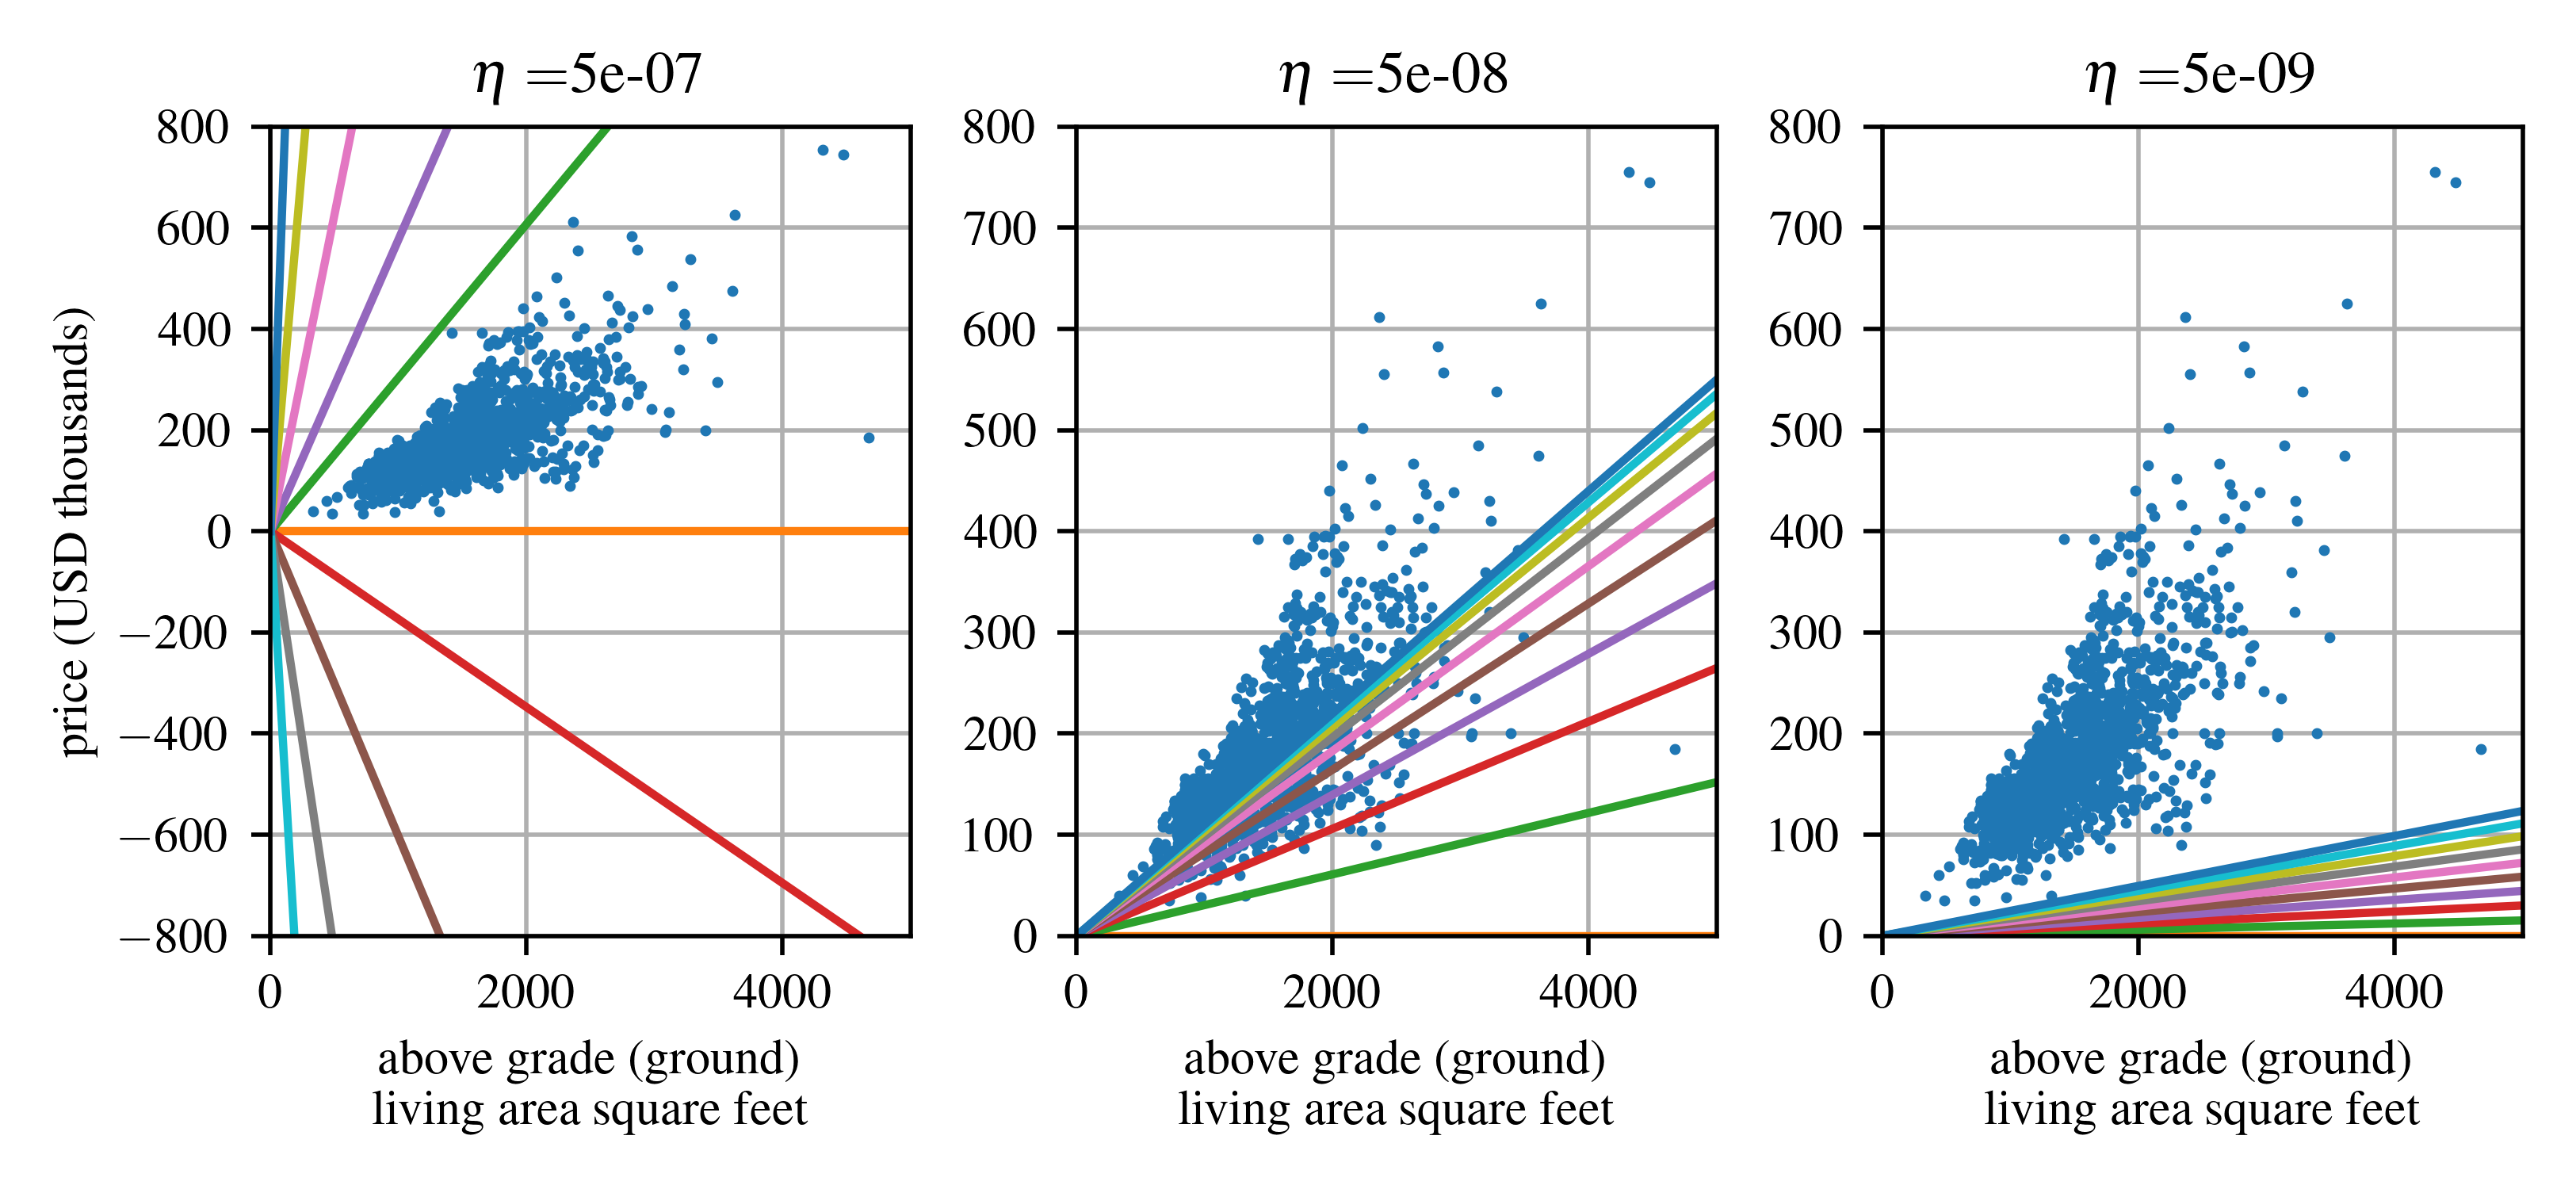
\includegraphics[width=6.5in]{../figures/Ames_learning_rates.png}
			\caption{The effects of different learning rates on the gradient descent algorithms, showing: (a)~too high ($\eta = 5e-07$); (b)~about right ($\eta = 5e-08$), and; (c)~too low ($\eta = 5e-09$).}
			\label{fig:learning_rates}
		\end{figure}


Figure~\ref{fig:learning_rates} highlights the impact of the learning rate on gradient descent.  
Figure~\ref{fig:learning_rates}(a) With a very large step size, \(\eta = 5\times10^{-7}\), each update overshoots the minimum so the algorithm diverges rather than converging.  
Figure~\ref{fig:learning_rates}(b) Using \(\eta = 5\times10^{-8}\) provides a balanced step size; the cost decreases just right~\protect\footnotemark[1] and the algorithm reaches the optimum in only a few iterations.  \footnotetext[1]{Pyle, K. ``Goldilocks and the three bears.'' Mother's Nursery Tales (1918): 207-213.} 
Figure~\ref{fig:learning_rates}(c) A small step size, \(\eta = 5\times10^{-9}\), keeps the algorithm moving toward the minimum yet progress is slow, requiring many more iterations to achieve the same result.


	




To identify an appropriate learning rate, a grid search can be employed. It is advisable to limit the number of iterations during grid search to avoid models that are too slow to converge.

Determining the correct number of iterations is also crucial. If set too low, the algorithm may stop far from the optimal solution. Conversely, overly high settings lead to unnecessary computations after convergence. A practical approach is to allow a large number of iterations but to halt the algorithm when the gradient vector's norm shrinks to below a small threshold $\epsilon$ (known as the tolerance), indicating proximity to the minimum.



\subsubsection{Stochastic Gradient Descent}


\begin{figure}[H]
	\centering
	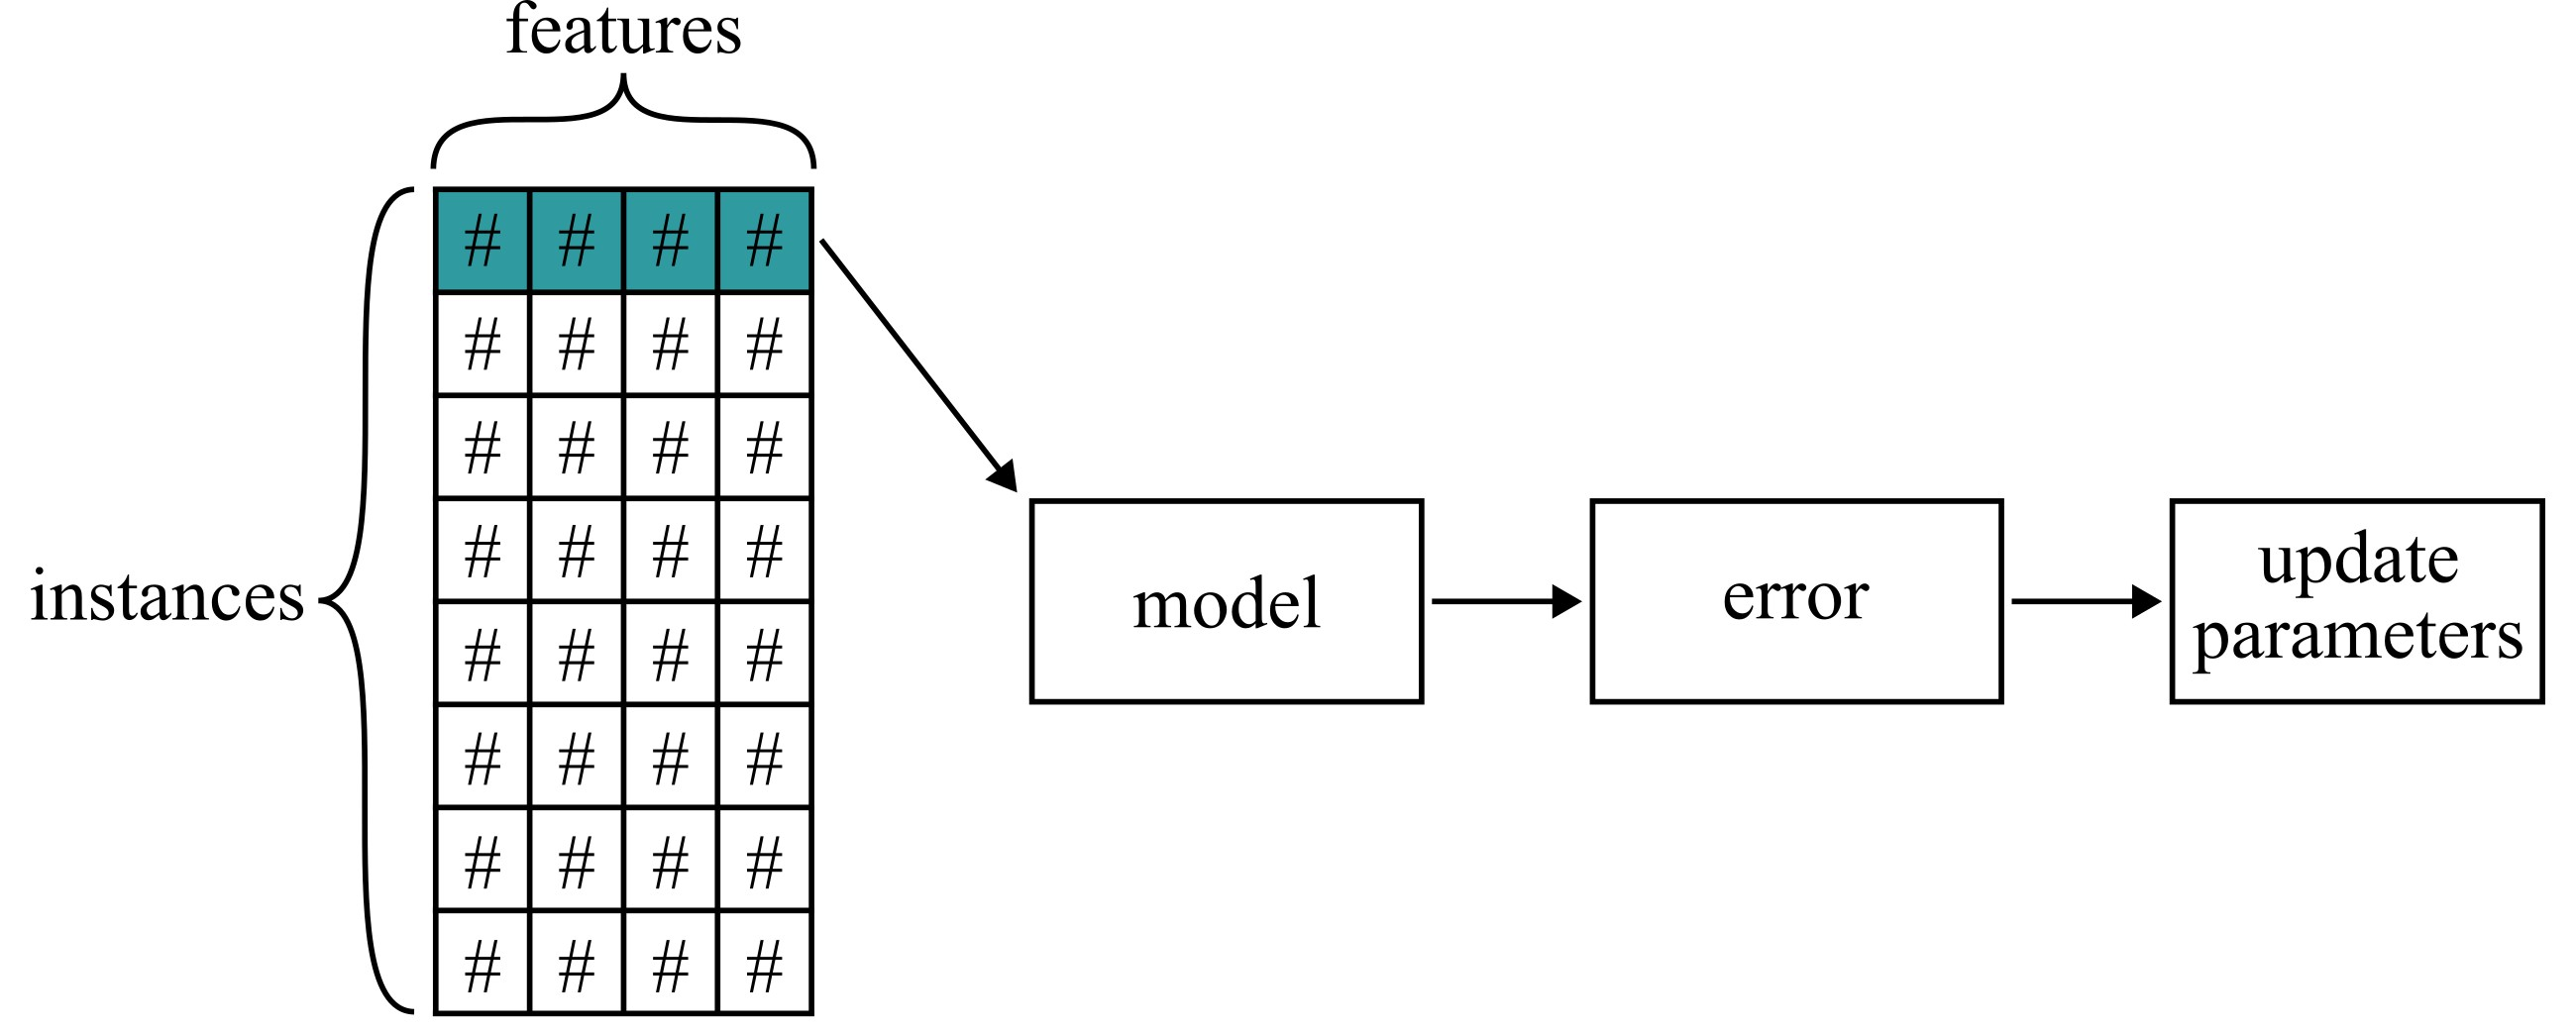
\includegraphics[width=5.4in]{../figures/gradient_descent_stochastic}
	\caption{Flowchart of Stochastic Gradient Descent.}
	\label{fig:gradient_descent_stochastic}
\end{figure}
Stochastic Gradient Descent (SGD) updates the model parameters after evaluating each individual training sample $x^{(i)}$ and its corresponding label $y^{(i)}$, which stands in contrast to batch gradient descent that uses the entire dataset for each update. The update rule for SGD can be expressed as:

\begin{equation}
\theta^{(\text{next step})} = \theta - \eta \nabla_\theta J(\theta; x^{(i)}; y^{(i)})
\end{equation}

While batch gradient descent tends to perform unnecessary recalculations for large datasets by reevaluating gradients for similar examples with each update, SGD eliminates this inefficiency by updating parameters incrementally. Consequently, SGD is generally faster and adaptable for online learning.

Due to its frequent and individual updates, SGD exhibits high variance in the objective function, causing significant fluctuations as illustrated in Fig.~\ref{fig:stochastic_gradient_descent_target}(b).


\begin{figure}[H]
	\centering
	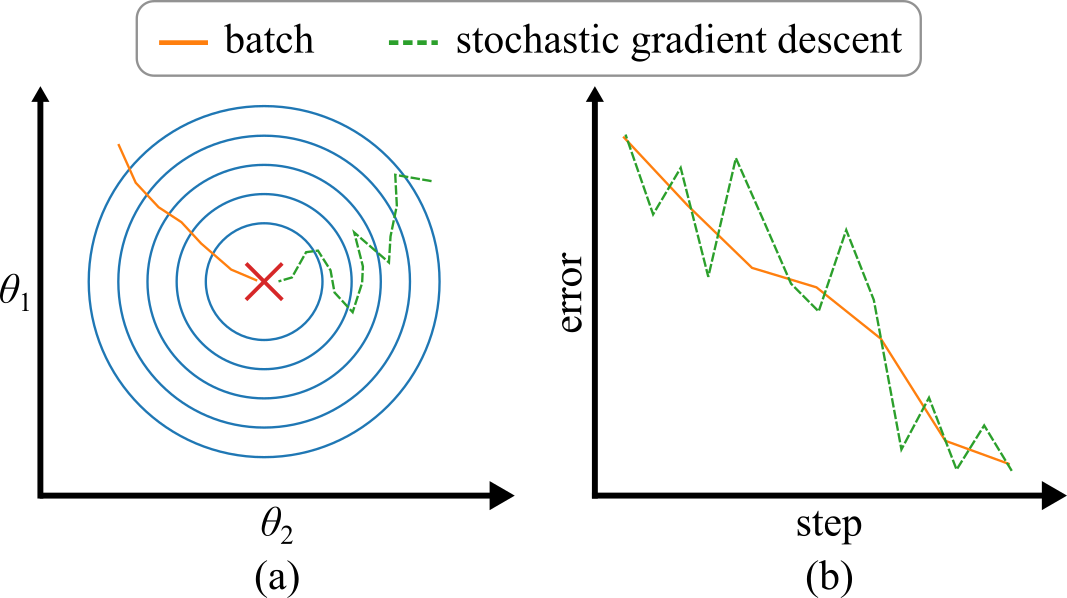
\includegraphics[]{../figures/stochastic_gradient_descent_target}
	\caption{Comparison of the iterative performance of  batch and Stochastic Gradient Descent, showing: (a) how they move towards their target, and (b) the error of each method for comparable steps.}
	\label{fig:stochastic_gradient_descent_target}
\end{figure}






\subsubsection{Mini-batch Gradient Descent}


\begin{figure}[H]
	\centering
	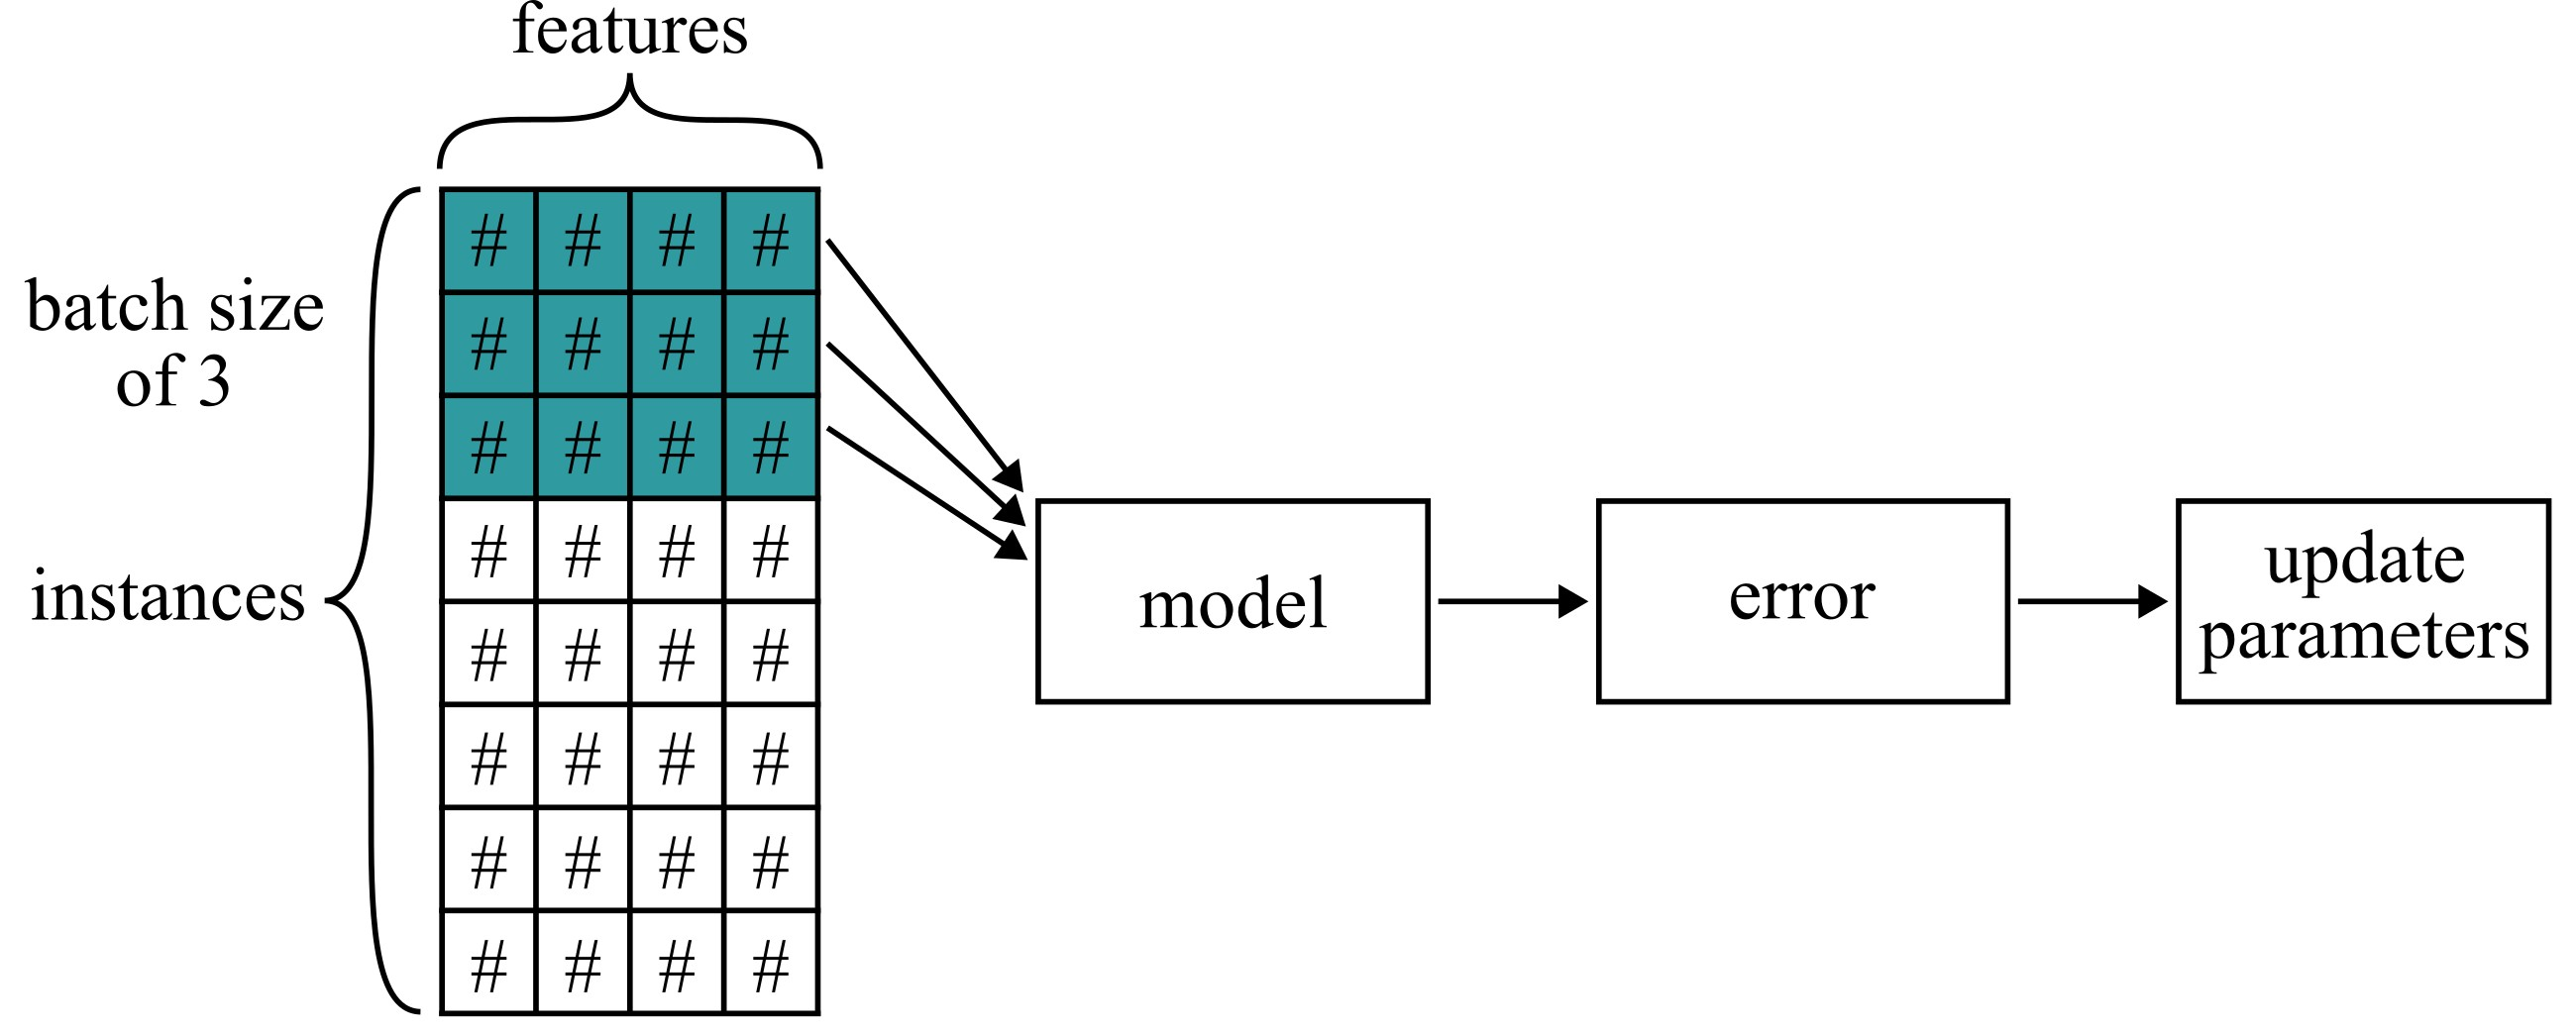
\includegraphics[width=5.4in]{../figures/gradient_descent_mini_batch}
	\caption{Flowchart of Mini-batch Gradient Descent.}
	\label{fig:gradient_descent_mini_batch}
\end{figure}


\begin{equation}
\theta^{(\text{next step})} = \theta - \eta \nabla_\theta J(\theta; x^{(i:i+n)}; y^{(i:i+n)})
\end{equation}

The final Gradient Descent algorithm we will discuss is Mini-batch Gradient Descent. This method combines elements of both Batch and Stochastic Gradient Descent: rather than calculating gradients using the entire training set (as in Batch GD) or a single instance (as in Stochastic GD), Mini-batch GD computes gradients using small, randomly selected subsets of instances known as minibatches. One significant benefit of Mini-batch GD over Stochastic GD is the improved performance from hardware-optimized matrix operations, particularly on GPUs.

Mini-batch GD's trajectory through parameter space tends to be more stable compared to the often erratic path of SGD, especially with larger minibatches. This stability typically brings Mini-batch GD closer to the minimum than SGD. However, Mini-batch GD might struggle more with escaping local minima in scenarios prone to such issues, which is less of a concern in Linear Regression. Figure~\ref{fig:Comparing_gradient_descent_methods} illustrates the trajectories of these three Gradient Descent techniques during training. While Batch GD precisely reaches the minimum, Stochastic GD and Mini-batch GD tend to oscillate nearby. It is important to note, however, that while Batch GD is slow in taking steps, both Stochastic GD and Mini-batch GD could also effectively reach the minimum with an appropriate learning rate schedule.




\subsubsection{Feature Scaling}

The cost function can resemble an elongated bowl if the feature scales vary significantly. Figure~\ref{fig:gradient_descent_5} illustrates the effect of feature scaling on Gradient Descent, comparing equal scaling of features (on the left) to disparate scaling (on the right).

\begin{figure}[H]
    \centering
    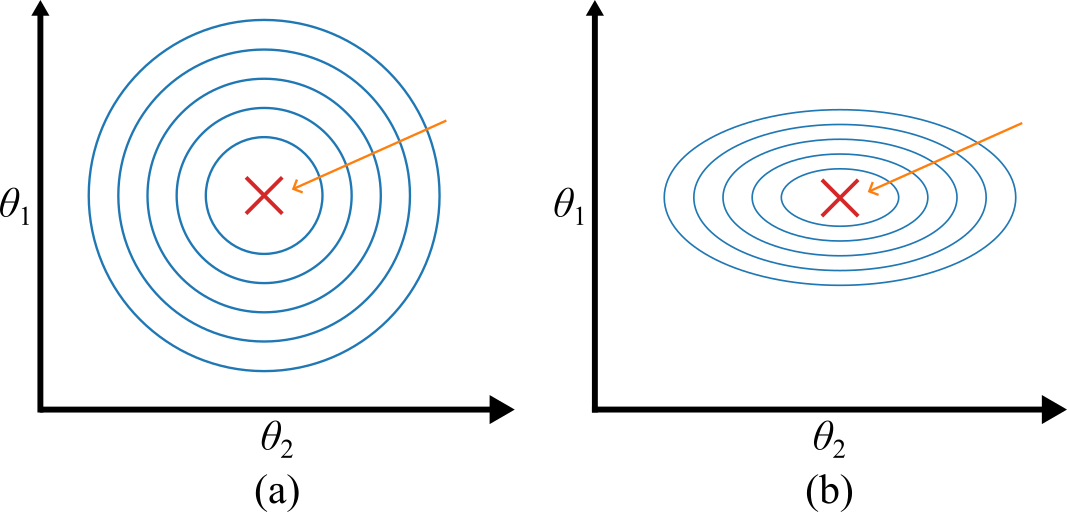
\includegraphics[]{../figures/gradient_descent_5.png }
    \caption{Gradient descent on a 2D surface for parameters that are: (a) equally scaled, and (b) unequally scaled.}
    \label{fig:gradient_descent_5}
\end{figure}

In figure~\ref{fig:gradient_descent_5}(a), Gradient Descent progresses directly towards the minimum, reaching it swiftly. However, in figure~\ref{fig:gradient_descent_5}(b) it initially moves almost orthogonally to the direction of the global minimum, followed by a lengthy traverse down a nearly flat valley, significantly delaying the convergence.

Training a model can be viewed as a search through the parameter space for the combination that minimizes the cost function. When additional parameters are introduced, this space gains extra dimensions, making the optimization task more challenging. In Ordinary Least Squares Linear Regression, however, the cost surface is convex and bowl-shaped, so any descent method is guaranteed to reach the global minimum. To normalize feature scales, two common methods are employed. The are Min-max scaling and Standardization. 
\begin{itemize}
\item \textbf{Min-max scaling}, often referred to as normalization, is straightforward: it rescales the data to a range of 0 to 1 by subtracting the minimum value and dividing by the range (max minus min).
\begin{equation}
\textbf{X}' = \frac{\textbf{X} - \textbf{X}_\text{min}}{\textbf{X}_\text{max} - \textbf{X}_\text{min}}
\end{equation}
Scikit-Learn offers \texttt{sklearn.preprocessing.MinMaxScaler} for this purpose.
\item \textbf{Standardization} differs significantly as it first subtracts the mean (resulting in a zero mean) and then divides by the standard deviation to achieve unit variance. This method does not limit values to a specific range, which can be problematic for certain algorithms, such as neural networks which often expect inputs between 0 and 1. However, standardization is less sensitive to outliers. For instance, if a median income is mistakenly recorded as 100, min-max scaling would compress all other values between 0 and 15 to between 0 and 0.15, whereas standardization would be minimally affected.
\begin{equation}
\textbf{X}' = \frac{\textbf{X} - \overline{\textbf{X}}}{\sigma}
\end{equation}
\texttt{sklearn.preprocessing.StandardScaler} is provided by Scikit-Learn for standardization.
\end{itemize}

\begin{mdframed}[middlelinewidth=0.5mm]
\begin{center}
\rd{WARNING}
\end{center}
It is crucial to apply scalers exclusively to the training data and not to the entire dataset, which includes the test set. This practice ensures that the model is not inadvertently exposed to test data during training. Once the scalers are fitted to the training data, they can then be used to transform the training set, the test set, and any new data subsequently encountered.
\end{mdframed}








\subsection{Polynomial Regression }



%\todo{Need to dicuss Bias and , include\_bias=False in sk.preprocessing.PolynomialFeatures. Why does this not need a bias? More math would be helpful. }


What if the underlying pattern of your data is more complex than a simple linear relationship? Consider the dataset shown in figure~\ref{fig:Polynomial_1} with non-linear characteristics (one feature across multiple instances), which typically can be modeled using a second-order polynomial
\begin{equation}
\hat{y}=ax^2+bx+c.
\label{eq:poly}
\end{equation}


\begin{figure}[H]
	\centering
	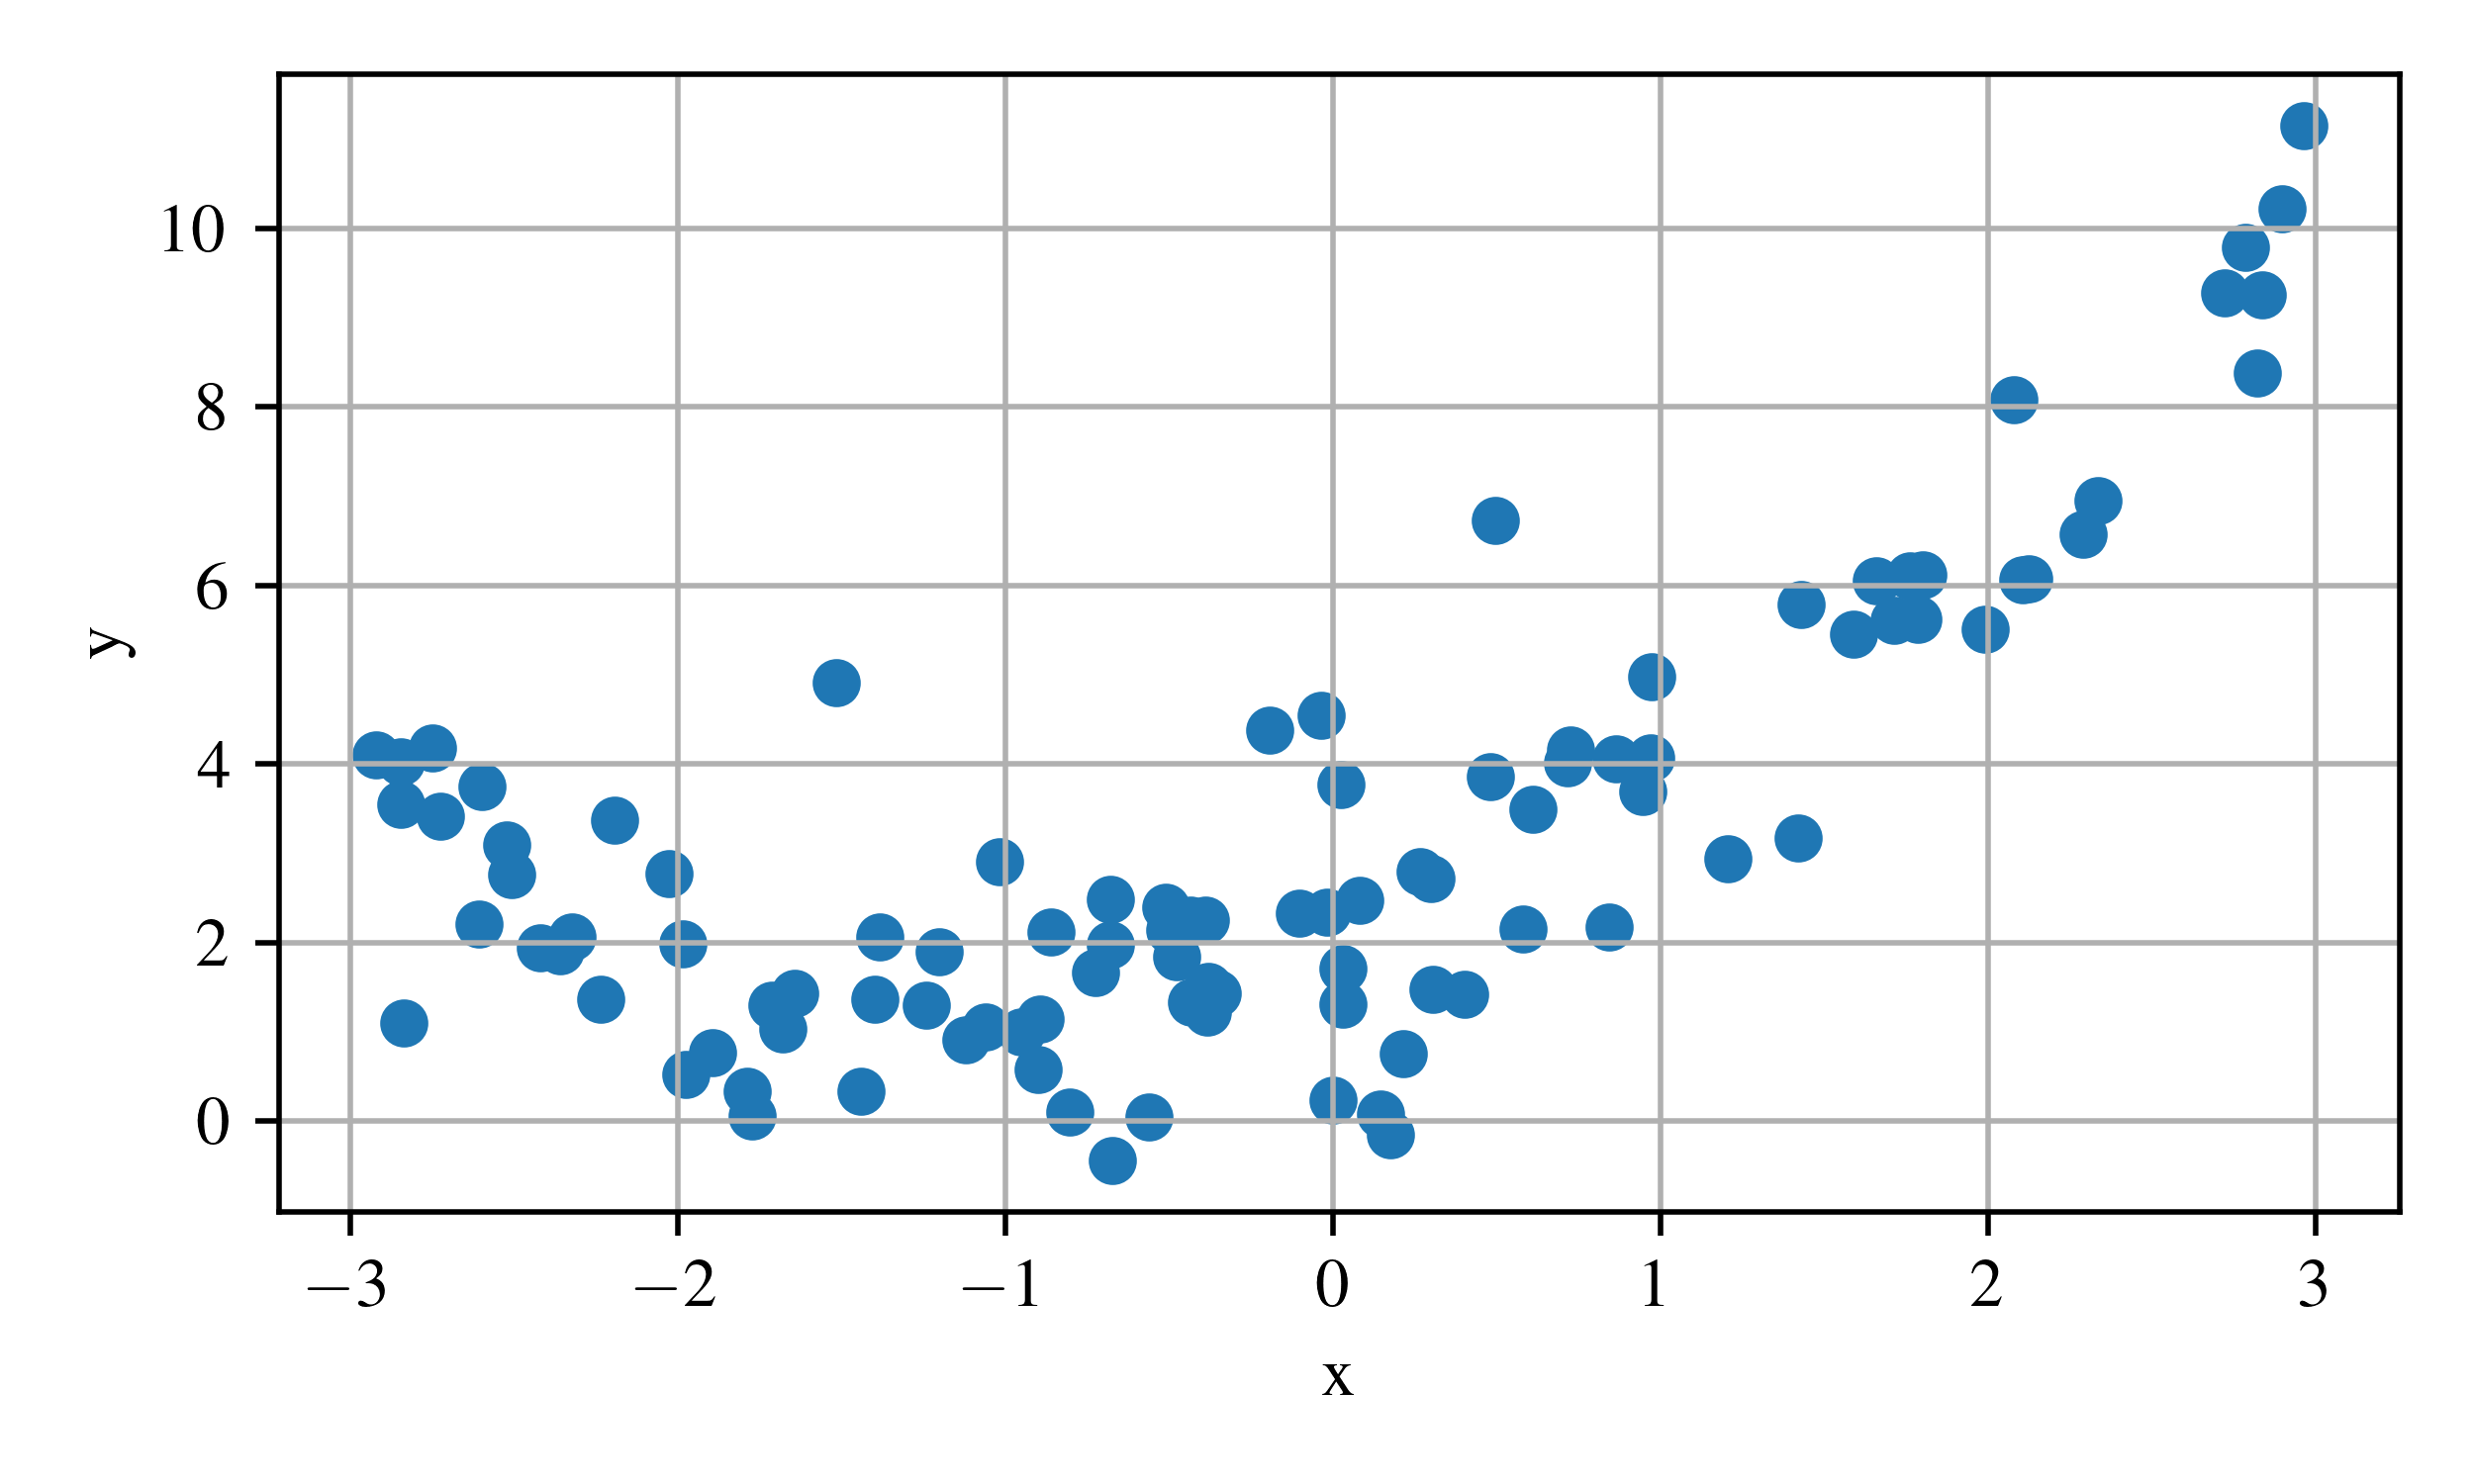
\includegraphics[width=4in]{../figures/polynomial_regression_1}
	\caption{Dataset derived from a 2\textsuperscript{nd}-order polynomial.}
	\label{fig:Polynomial_1}
\end{figure}

%\todo{need to talk about how this is only one feature, and we build off of that. }
%\url{https://medium.com/analytics-vidhya/understanding-polynomial-regression-5ac25b970e18}

A simple linear fit will under-perform, so you first enrich the training set by adding the squared term of each feature as an extra column; shown in figure~\ref{fig:Polynomial_2}. Although the model you train is still linear with respect to its parameters, it now operates on an augmented feature space and can represent the desired quadratic curve. This approach is called Polynomial Regression, and it extends naturally by including higher powers whenever more complex nonlinearities are present.


		\begin{figure}[H]
			\centering
			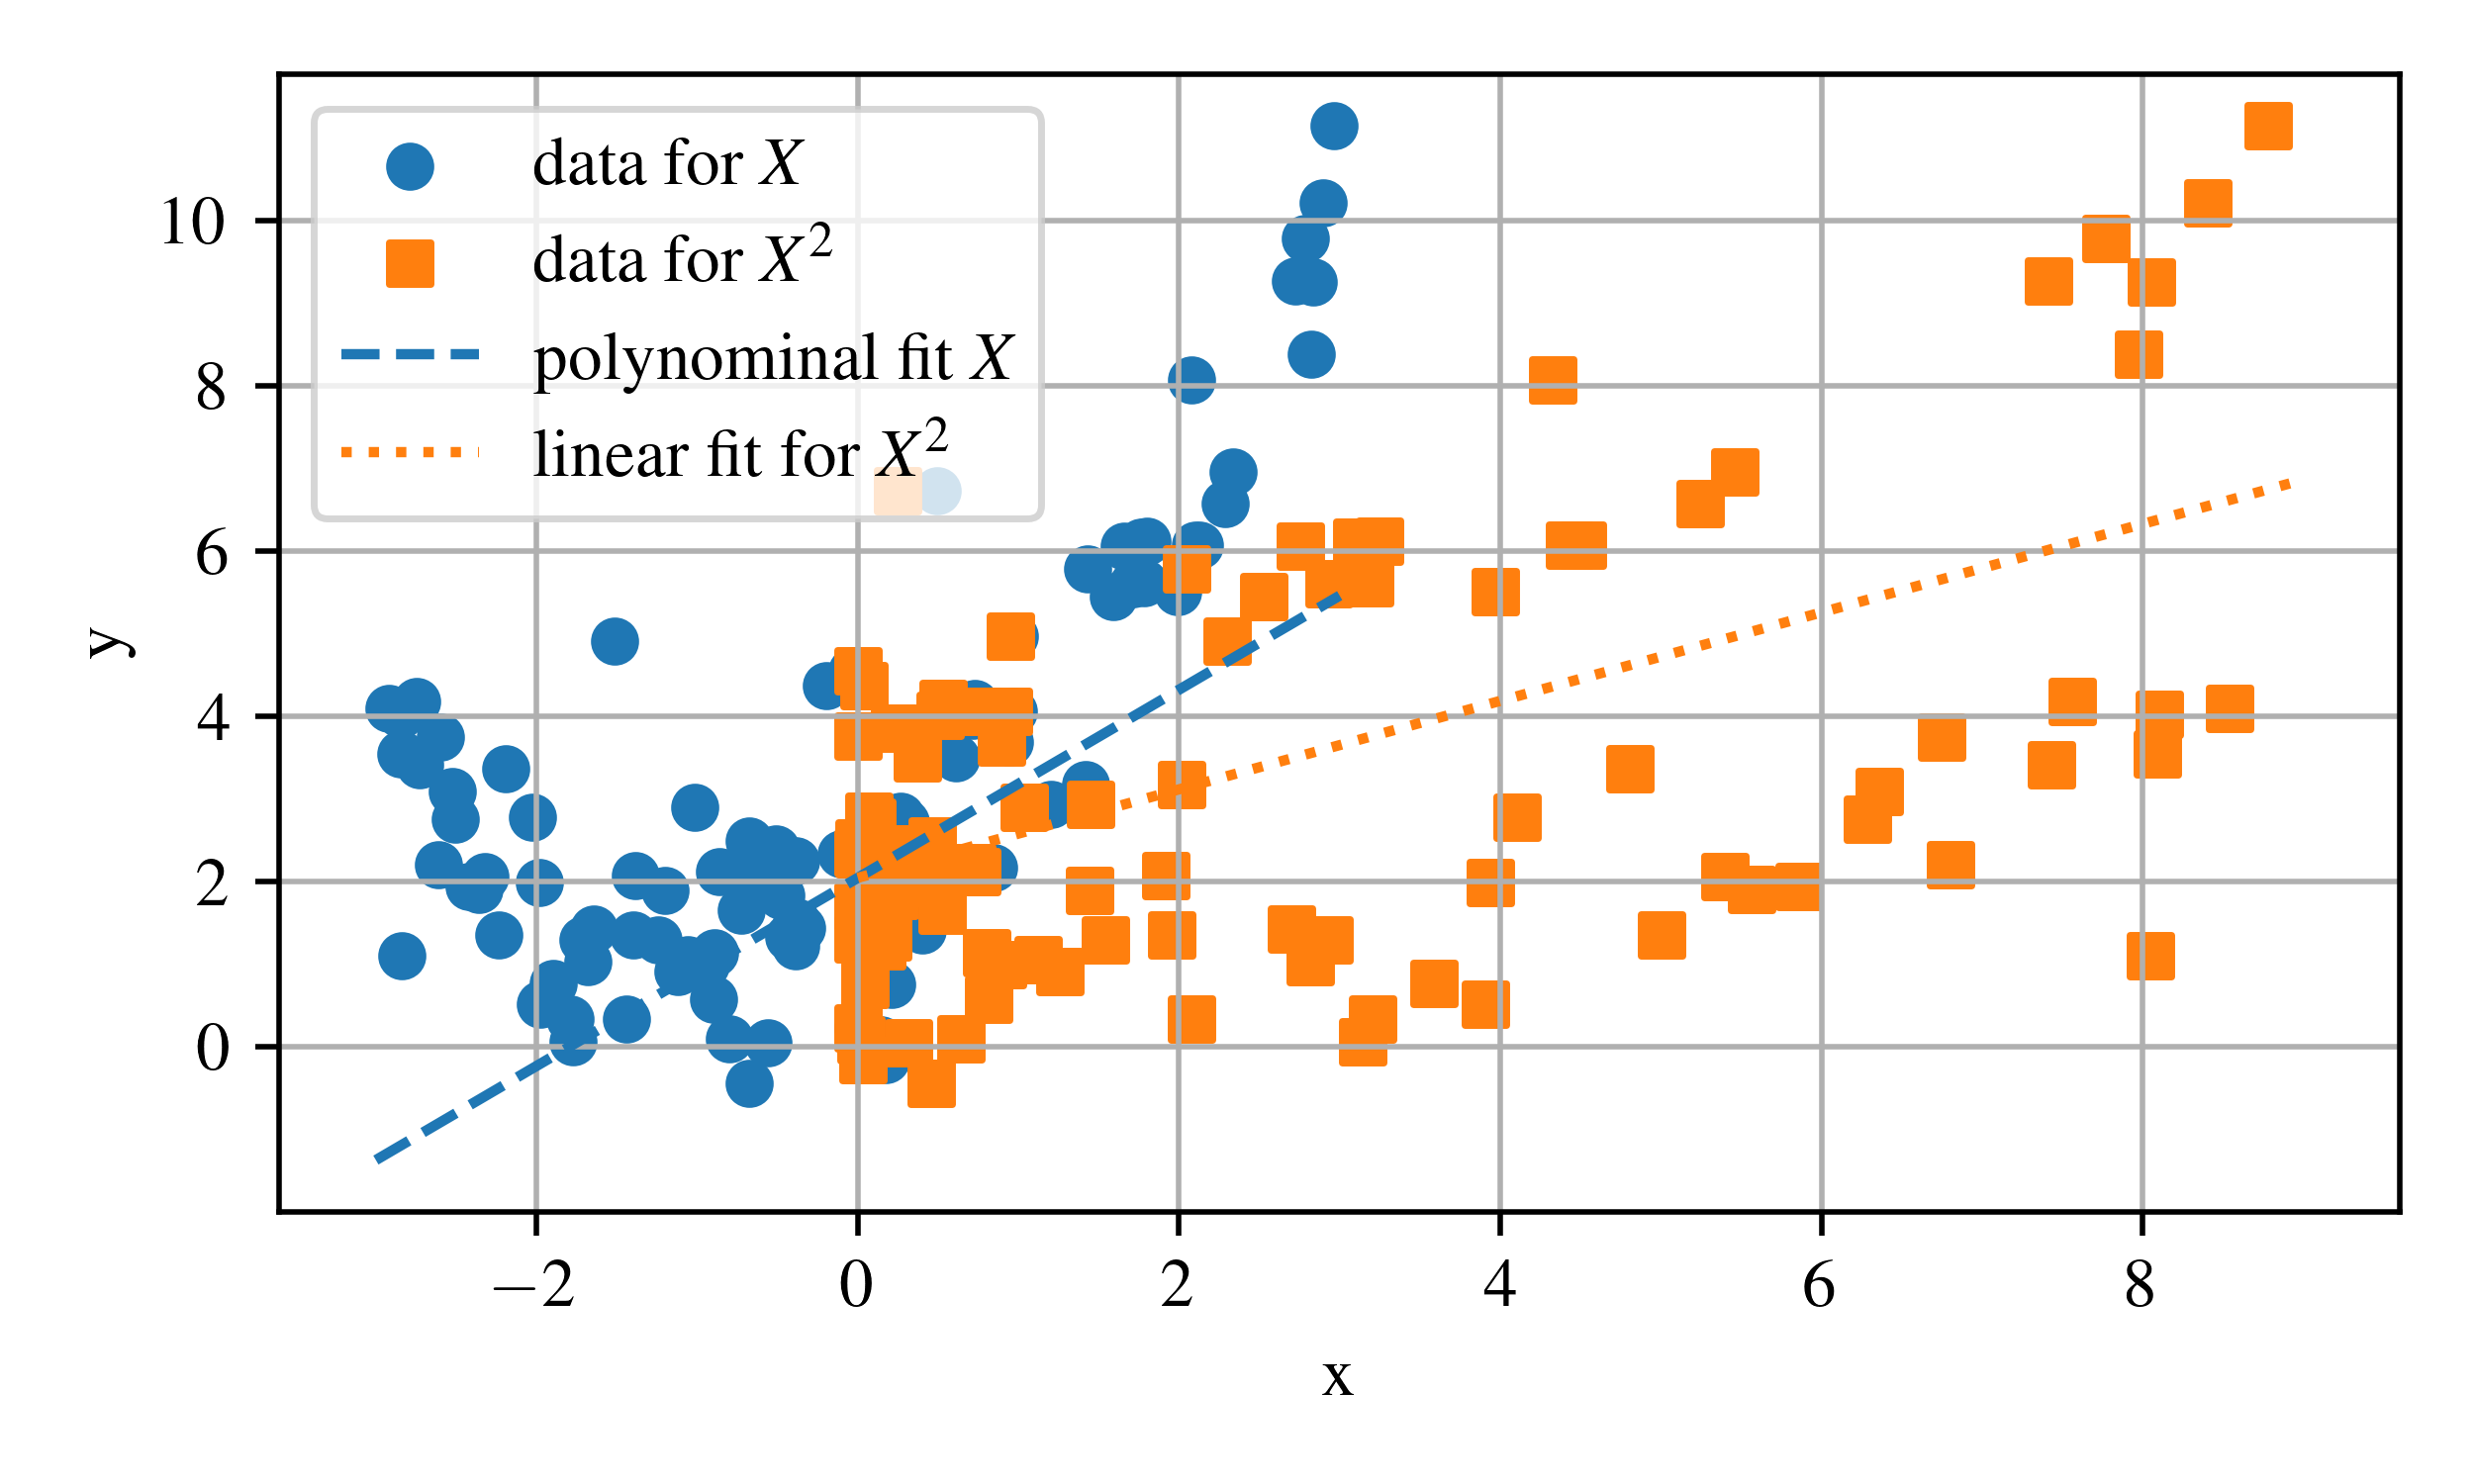
\includegraphics[width=4in]{../figures/polynomial_regression_2}
			\caption{Linear models fit to the individual features of a polynomial dataset.}
			\label{fig:Polynomial_2}
		\end{figure}

This data can then be incorporated into two linear models, where the slopes of the feature sets serve as the parameters for the base-line polynomial expression ($a$ and $b$ in Equation~\ref{eq:poly}) and the bias term is the offset ($c$ in Equation~\ref{eq:poly}). The results of such a polynomial fit is shown in figure~\ref{fig:Polynomial_3}.


		\begin{figure}[H]
			\centering
			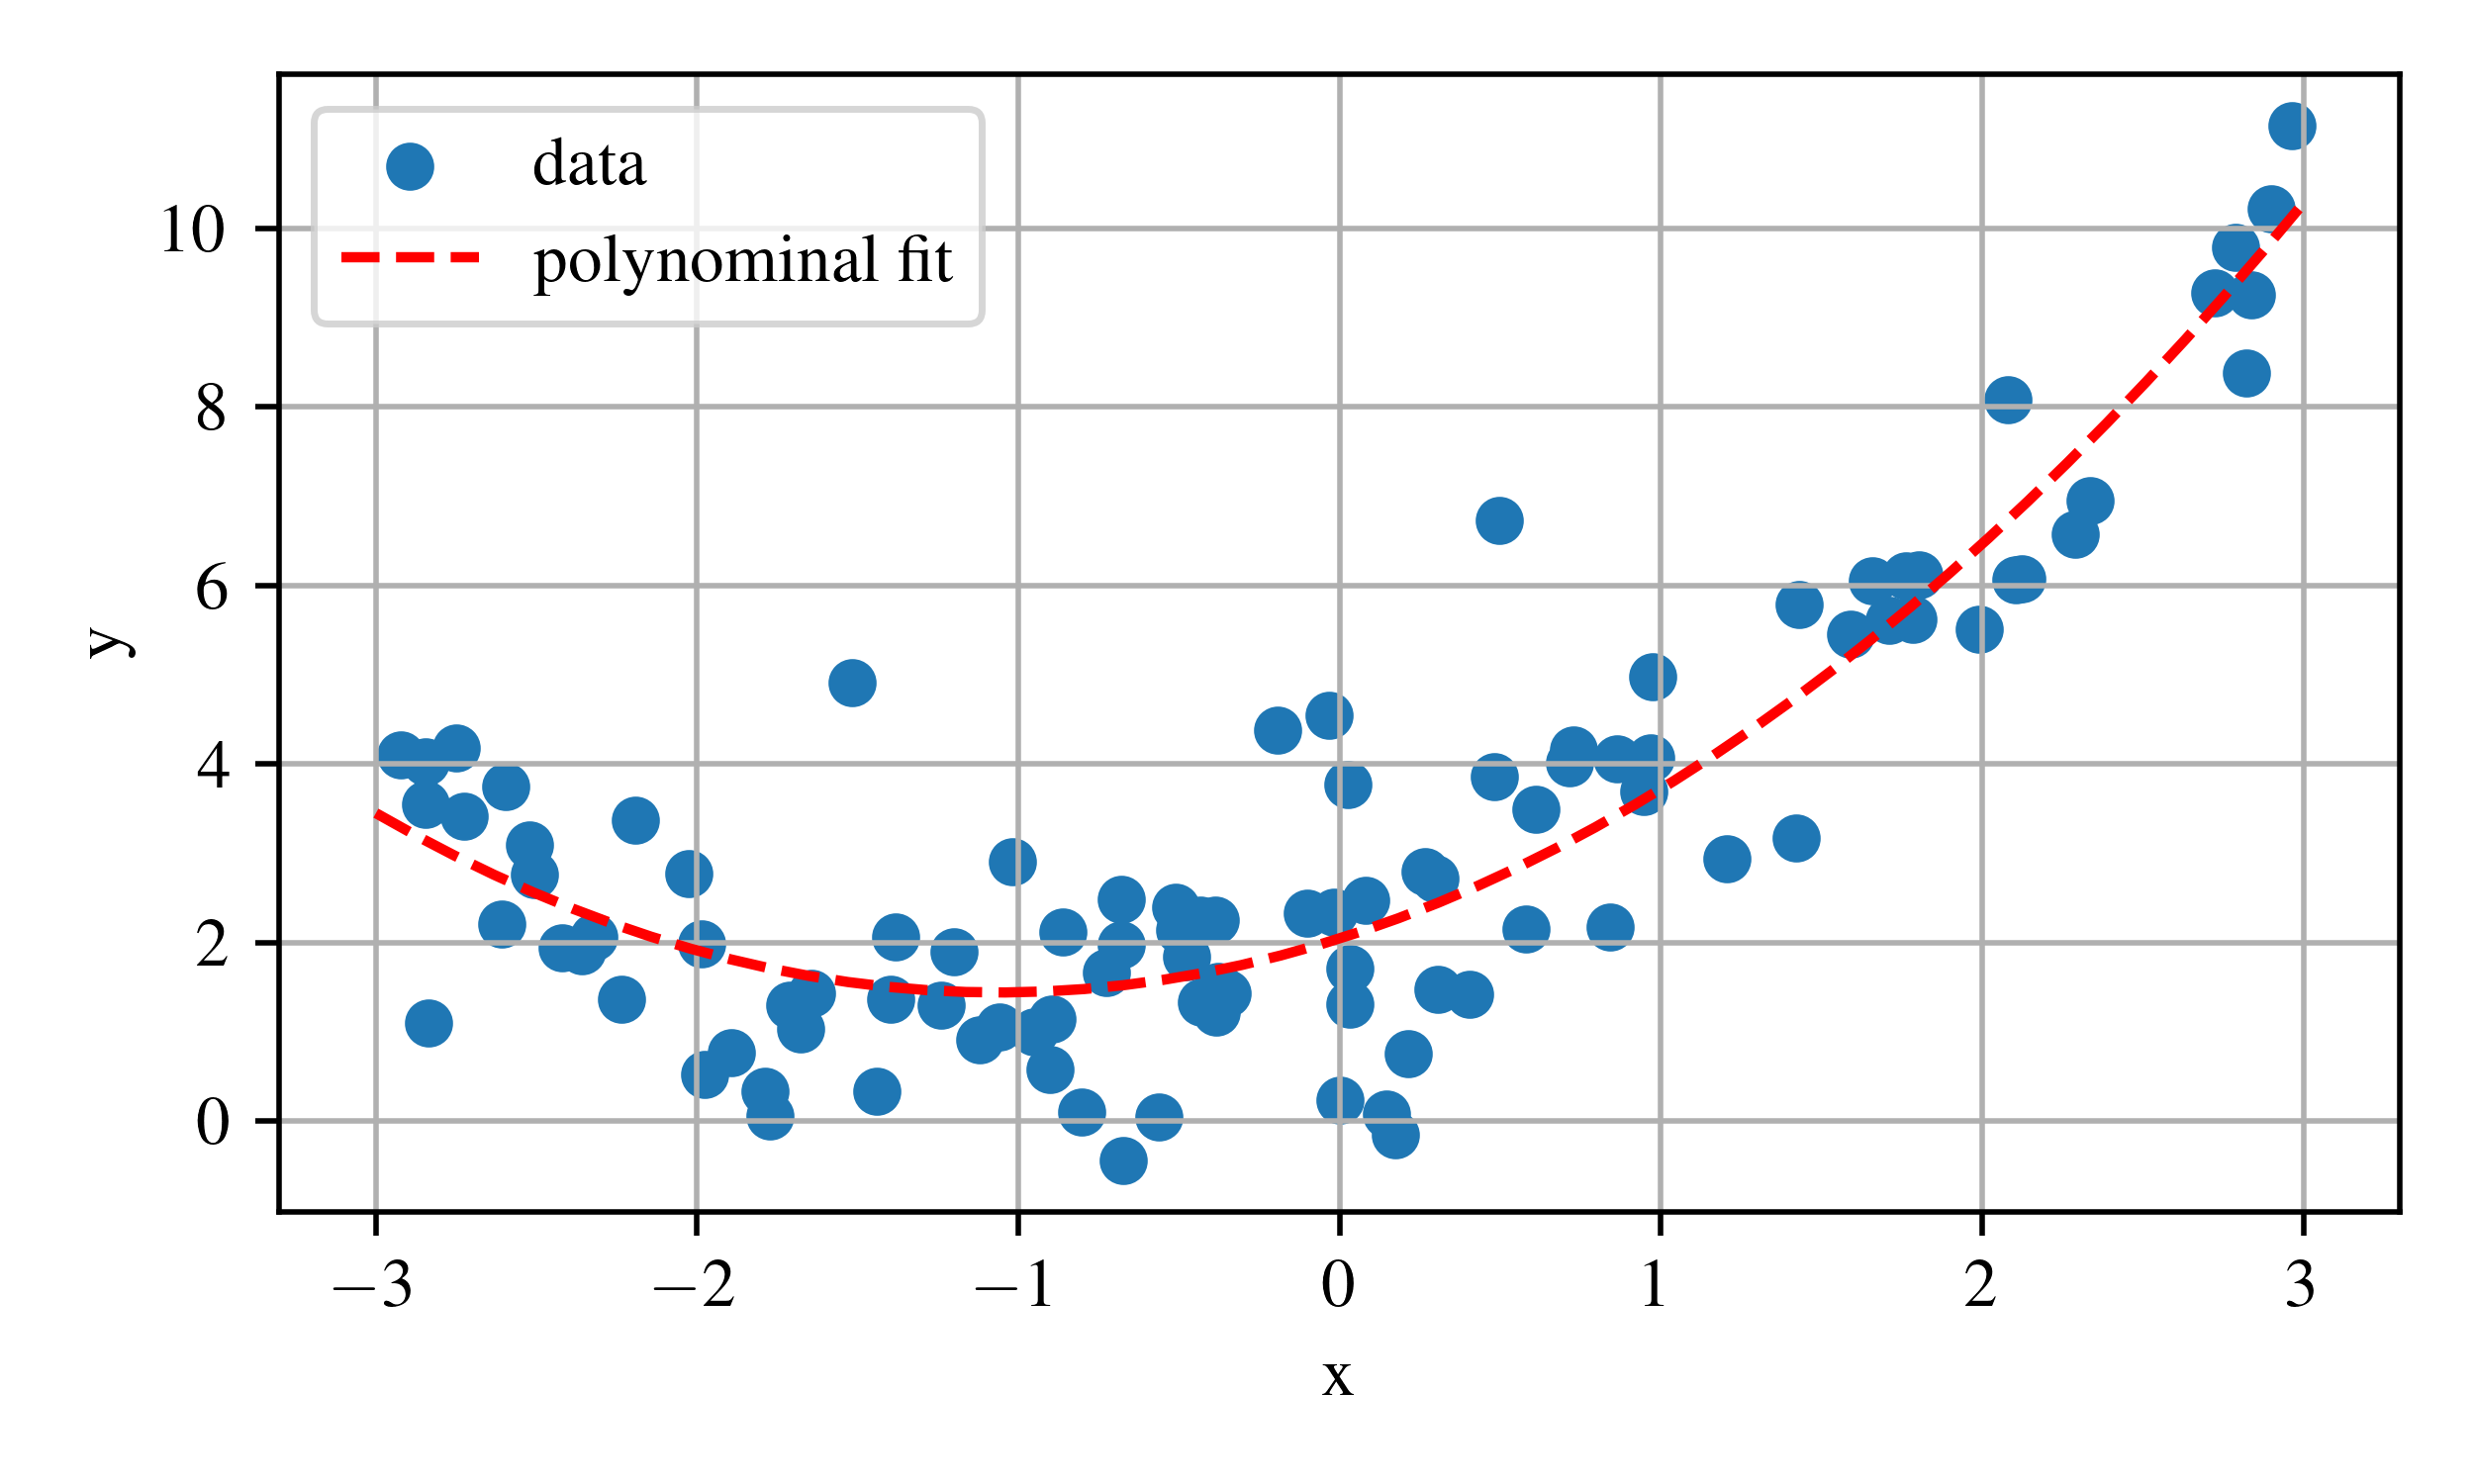
\includegraphics[width=4in]{../figures/polynomial_regression_3}
			\caption{Polynomial model fit to a dataset.}
			\label{fig:Polynomial_3}
		\end{figure}


It is important to note that Polynomial Regression can identify interrelationships between features in cases where multiple features exist, a capability beyond the scope of simple Linear Regression. This enhancement is enabled by \texttt{PolynomialFeatures}, which includes all possible combinations of features up to the specified degree. For instance, with two features $a$ and $b$, and a degree of 3, \texttt{PolynomialFeatures} would add not only $a^2, a^3, b^2,$ and $b^3$ but also the combined terms $ab, a^2b,$ and $ab^2$.



\begin{mdframed}[middlelinewidth=0.5mm]
\begin{center}
\rd{WARNING}
\end{center}
\texttt{PolynomialFeatures(degree=d)} expands an array with $n$ original features into one that includes $\frac{(n+d)!}{d!n!}$ features, accounting for all combinations of features up to the $d$-th degree. Here, $n!$ represents the factorial of $n$, calculated as $1 \times 2 \times 3 \times \cdots \times n$. Be cautious of the rapid increase in the number of features, known as combinatorial explosion!
\end{mdframed}

\begin{example}
\textbf{Polynomial Regression}

\noindent This example fits a non-linear dataset using polynomial regression by adding $x^2$ as an extra feature. It demonstrates how linear models can approximate curved relationships when polynomial terms are included, and shows the resulting fit compared to the original data.
\end{example}



\subsection{Training and Testing Data}

Training a predictive model on a dataset and then testing it with the same data is a fundamental error in methodology. Such a model could simply memorize the labels of the training samples, achieving perfect performance during training but failing to make any useful predictions on new, unseen data. This phenomenon is known as overfitting. To prevent this, it is standard practice in supervised machine learning to reserve a portion of the available data as a test set, denoted as $\textbf{X}_\text{test}$ and $\textbf{y}_\text{test}$.

		\begin{figure}[H]
			\centering
			
\includegraphics[]{../figures/training_test_datasets}
			\caption{Splitting data up into training and testing subsets.}
			\label{fig:training_test_datasets}
		\end{figure}


		\begin{figure}[H]
			\centering
			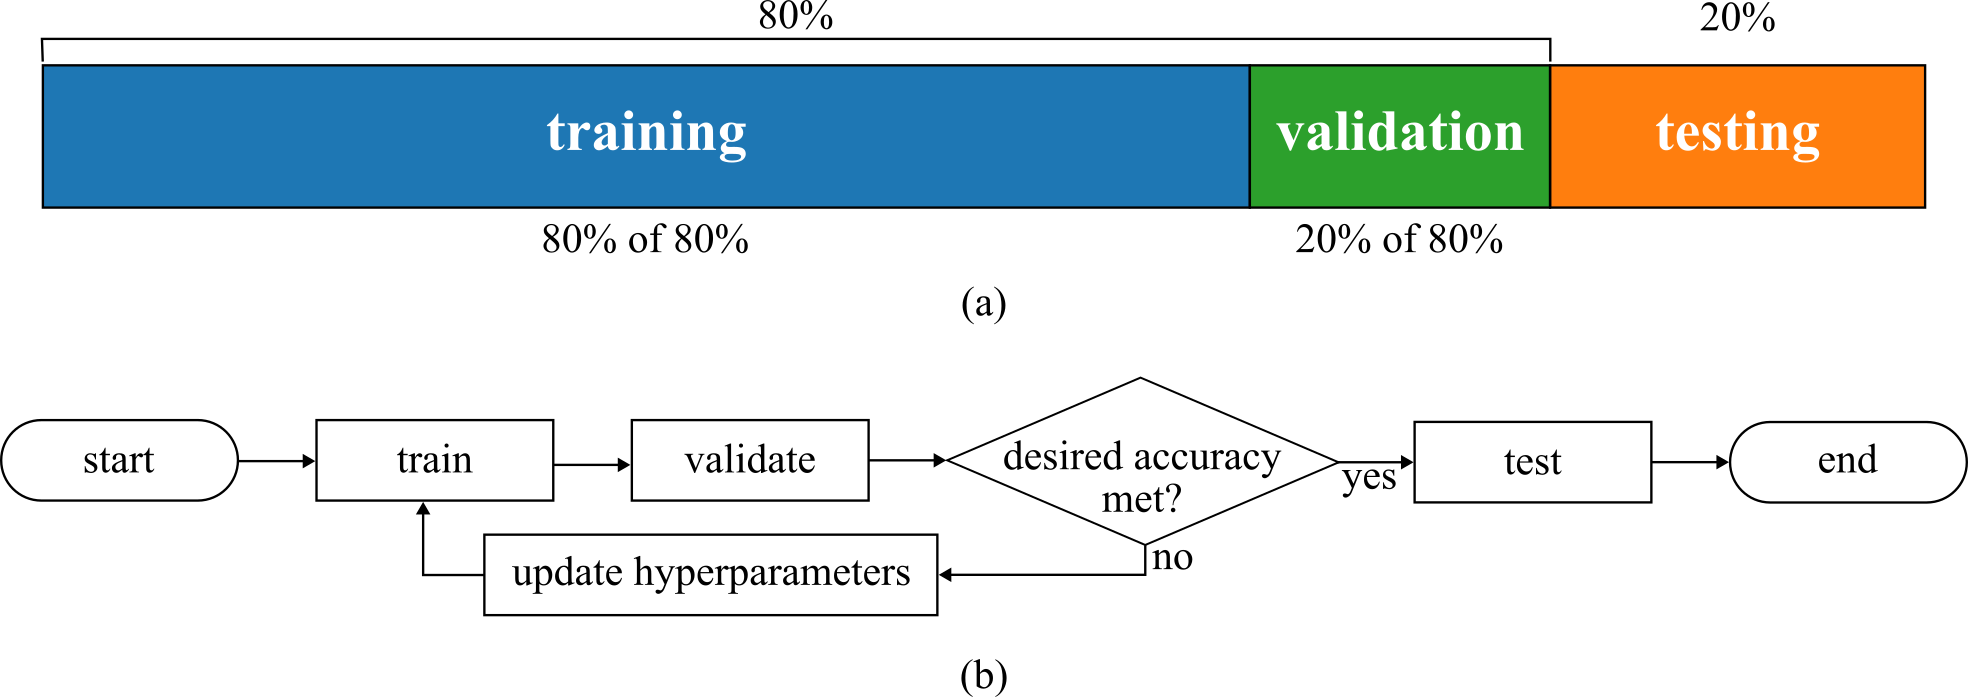
\includegraphics[]{../figures/training_validation_test_datasets}
			\caption{Splitting data up into training, validation, and testing subsets.}
			\label{fig:training_validation_test_datasets}
		\end{figure}


The function \texttt{sklearn.model\_selection.train\_test\_split} in scikit-learn randomly divides arrays or matrices into training and testing subsets.



\subsection{Pipelines}


Pipelines in scikit-learn streamline the process by sequentially applying a list of transformations followed by a final estimator to a dataset. Employing pipelines allows for the integration of multiple processing steps, which can then be cross-validated together while experimenting with various parameters. Fig.~\ref{fig:AutoML_diagram} illustrates a typical pipeline configuration in scikit-learn.



		\begin{figure}[H]
			\centering
			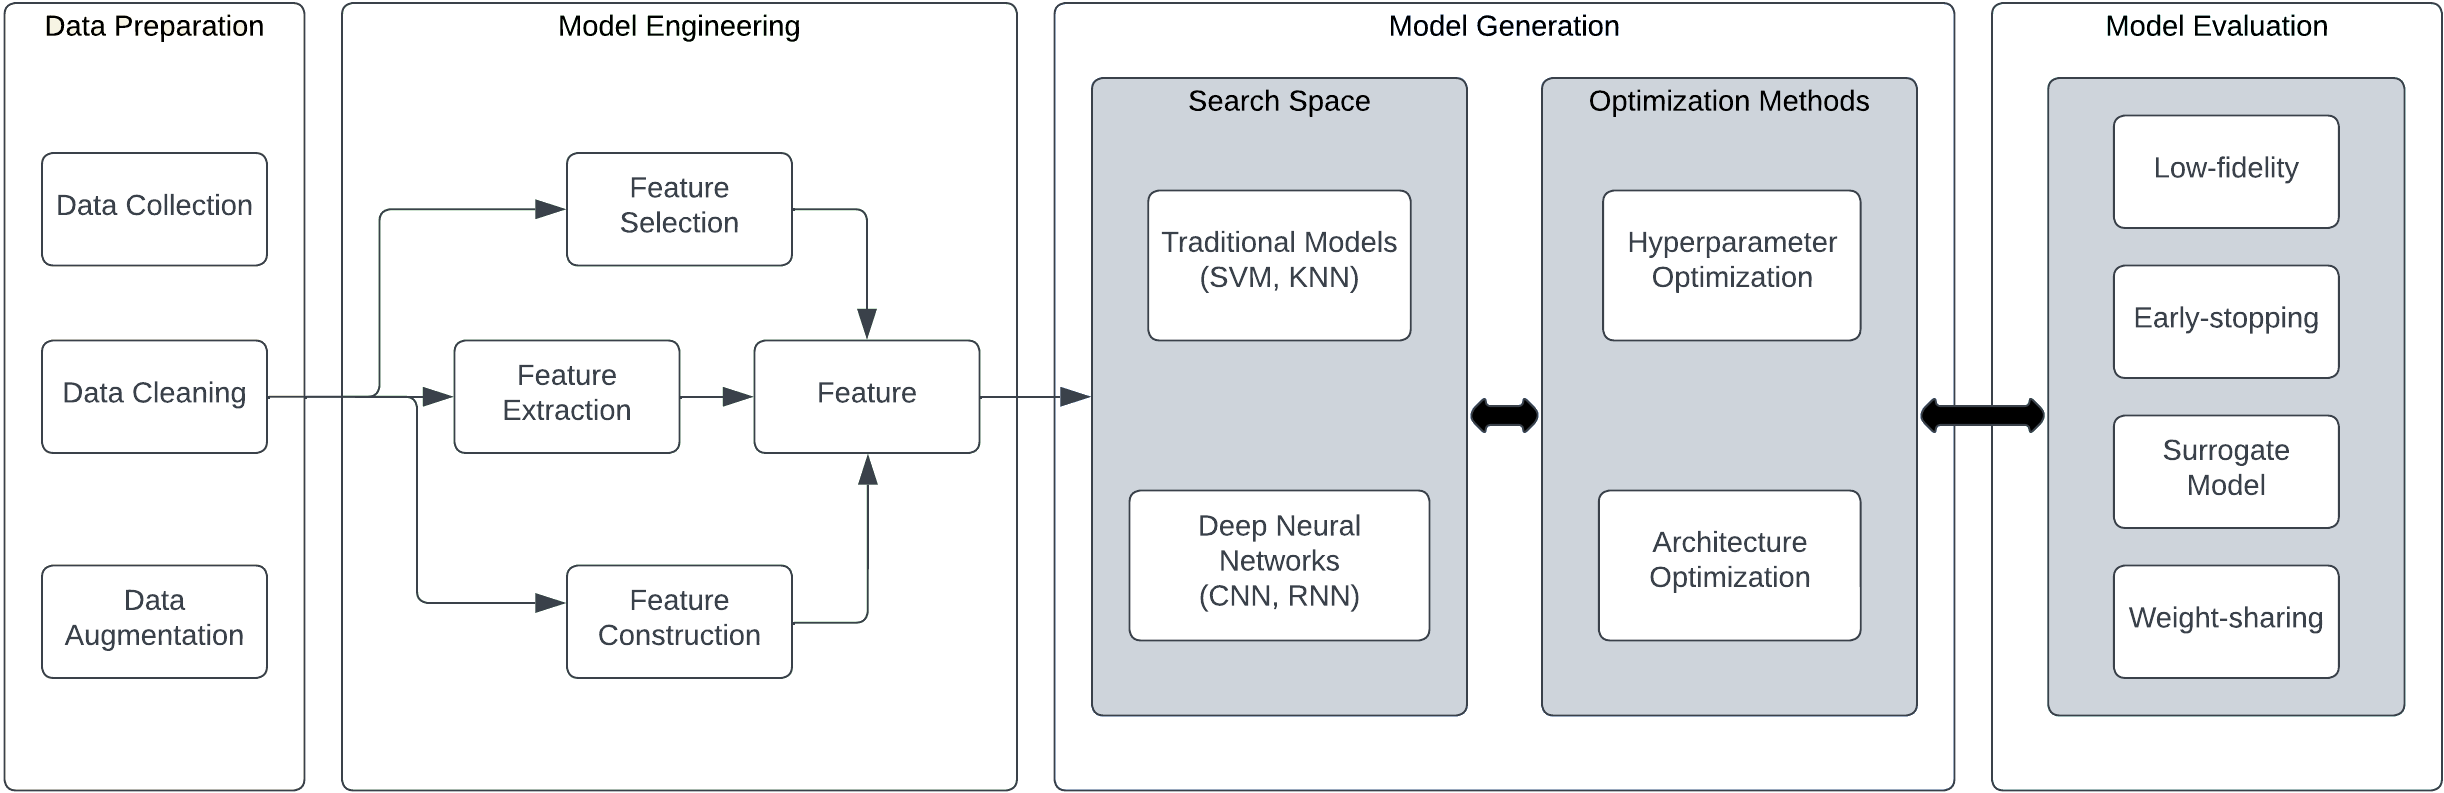
\includegraphics[width=6.5in]{../figures/AutoML_diagram}
			\caption{Pipeline setup for the automated deployment of pre-processing and modeling steps.\protect\footnotemark[1]}
			\label{fig:AutoML_diagram}
		\end{figure}


\footnotetext[1]{Modified from PopovaZhuhadar, CC BY-SA 4.0 $<$https://creativecommons.org/licenses/by-sa/4.0$>$, via Wikimedia Commons}

\subsection{Learning Curves}

Performing Polynomial Regression with a high degree typically allows for a closer fit to the training data compared to simple Linear Regression. For instance, Figure~\ref{fig:overfitting_1} demonstrates the application of a 30-degree polynomial model to a set of training data, contrasting it with both a linear model and a quadratic model (2\textsuperscript{nd}-degree polynomial). Observe how the 30-degree polynomial model contorts to closely match the training instances.
\begin{itemize}
\item The linear model exhibits underfitting.
\item The high-degree Polynomial Regression model drastically overfits the training data.
\item Among these, the quadratic model is likely to generalize best.
\end{itemize}
In this instance, the appropriateness of the quadratic model is clear since the data was initially generated using such a model. However, in real-world scenarios where the underlying function of the data is unknown, determining the optimal complexity for your model can be challenging. How can you ascertain whether your model is overfitting or underfitting the data?

\begin{figure}[h]
\centering
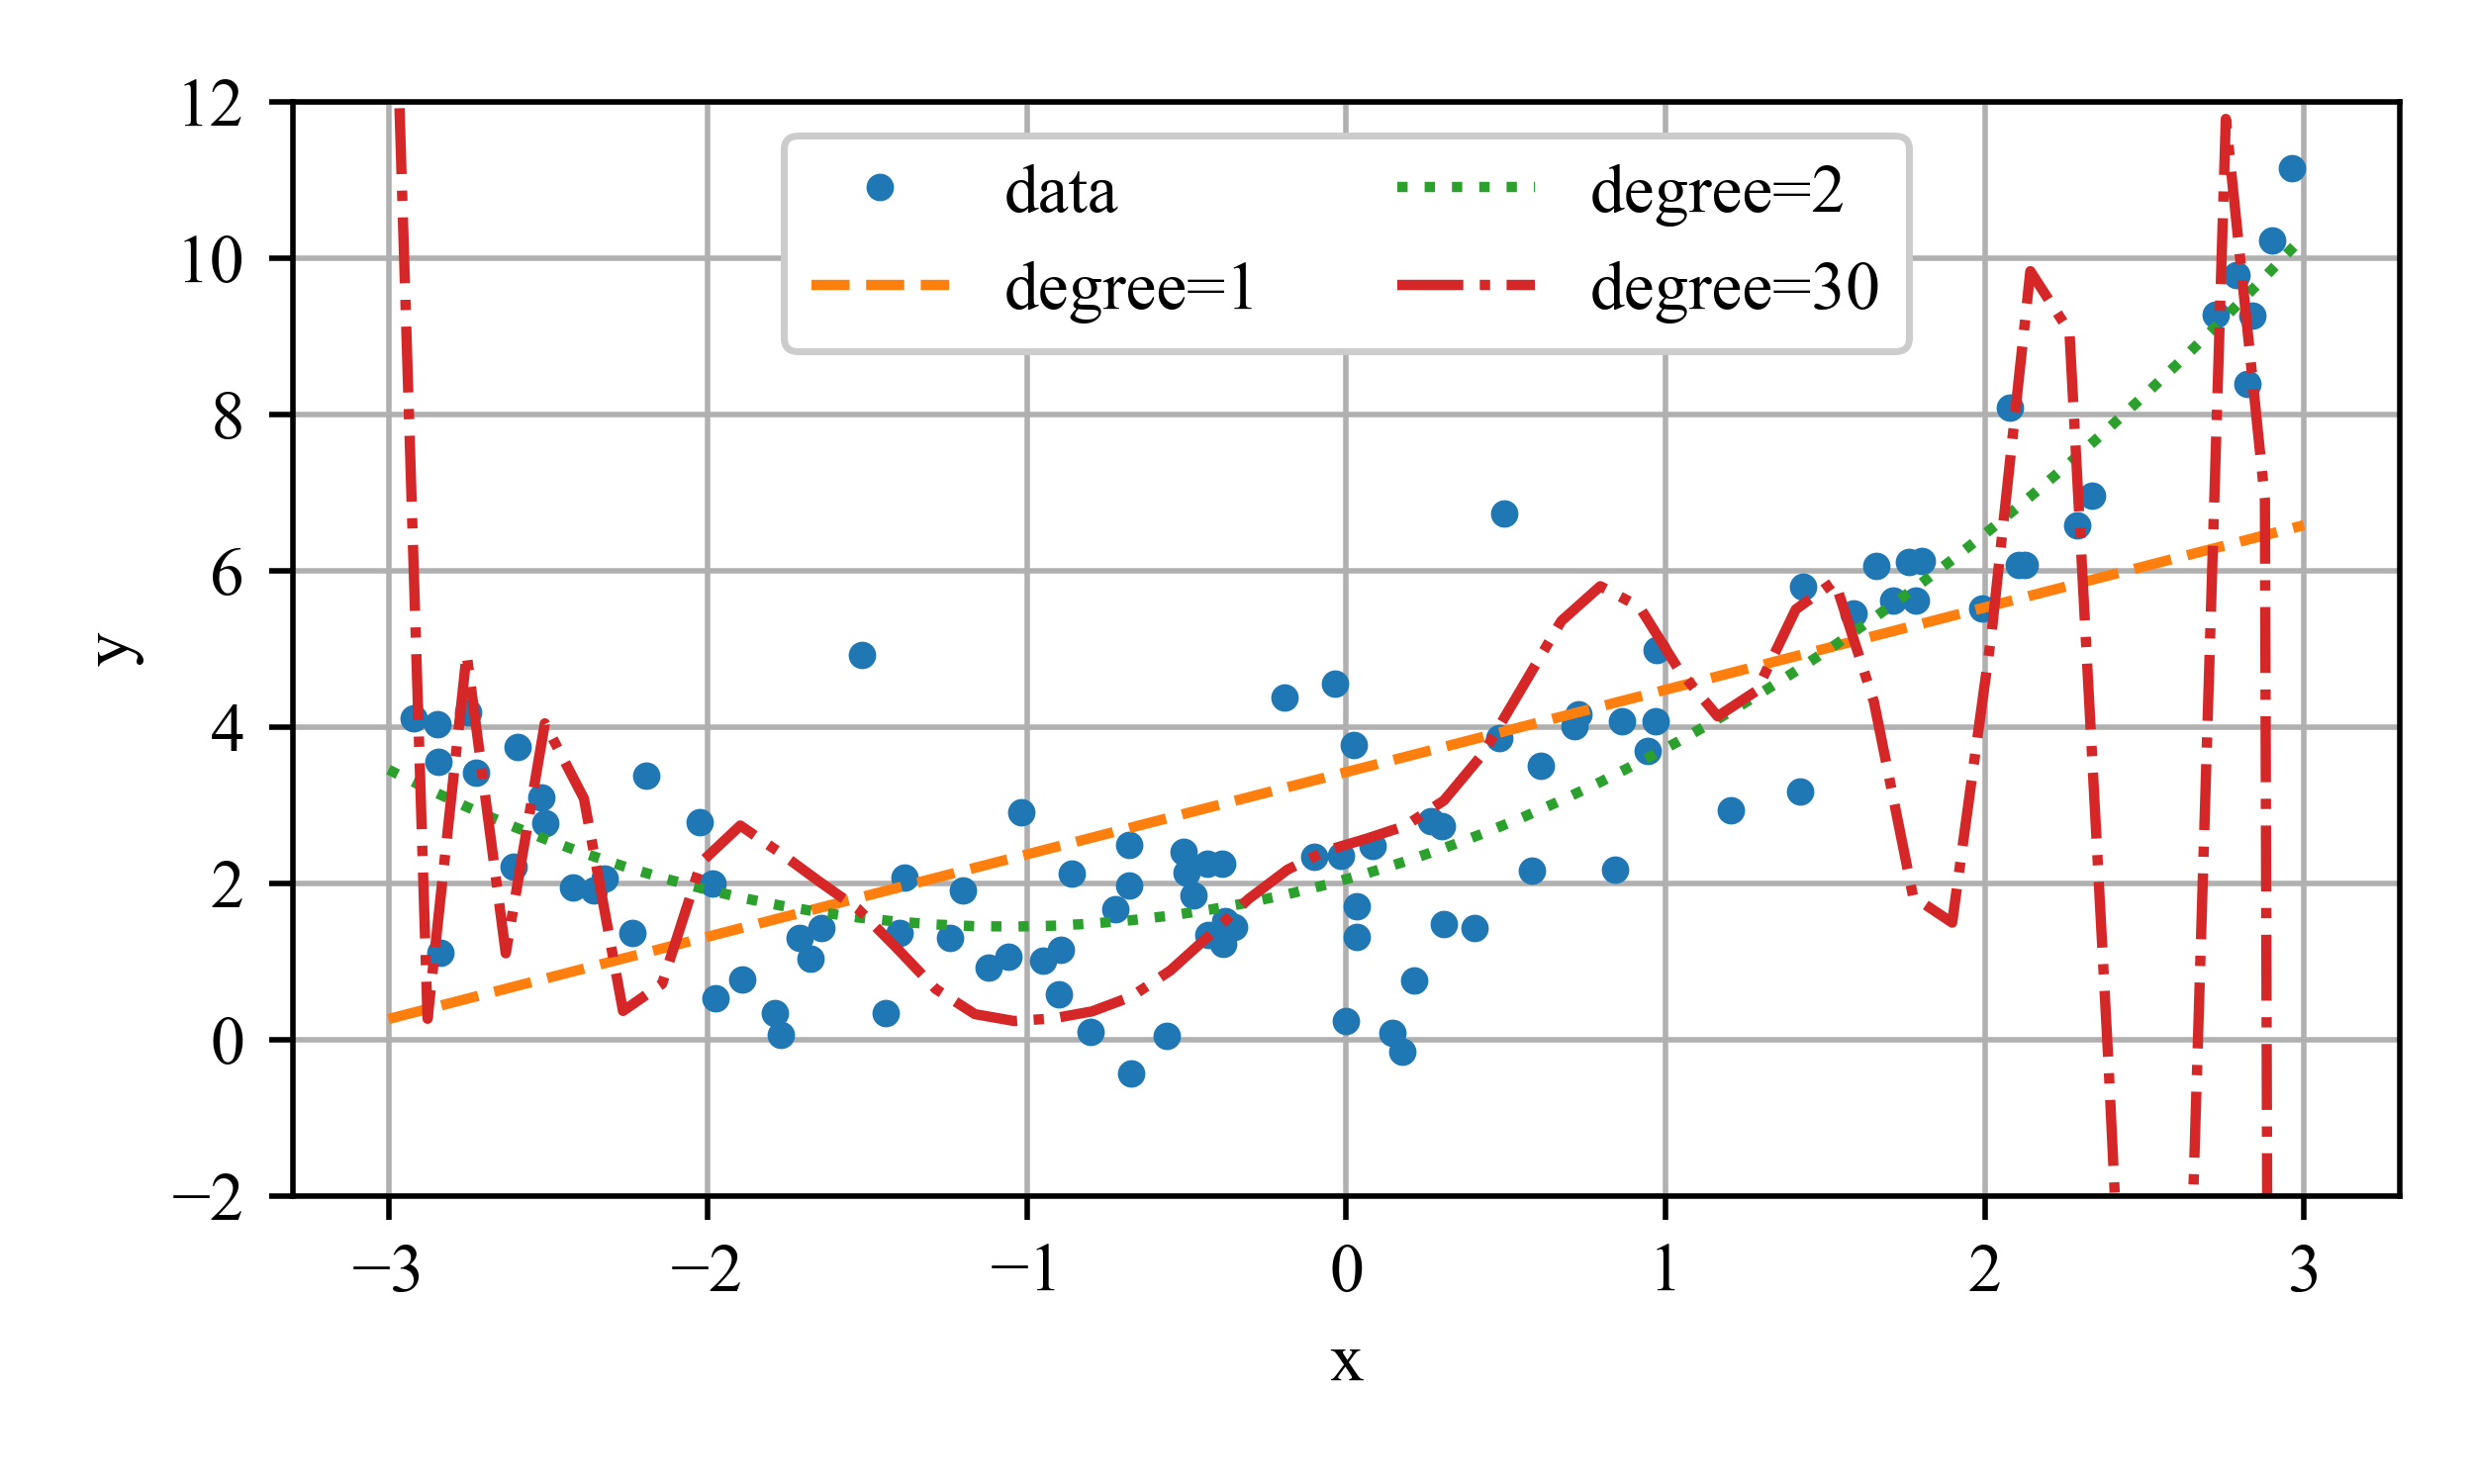
\includegraphics[]{../figures/overfitting_1.png}
\caption{Polynomial regression showing underfitting (degree=1), a respectable model fit (degree=2), and overfitting (degree=30).}
\label{fig:overfitting_1}
\end{figure}





\begin{figure}[H]
\centering
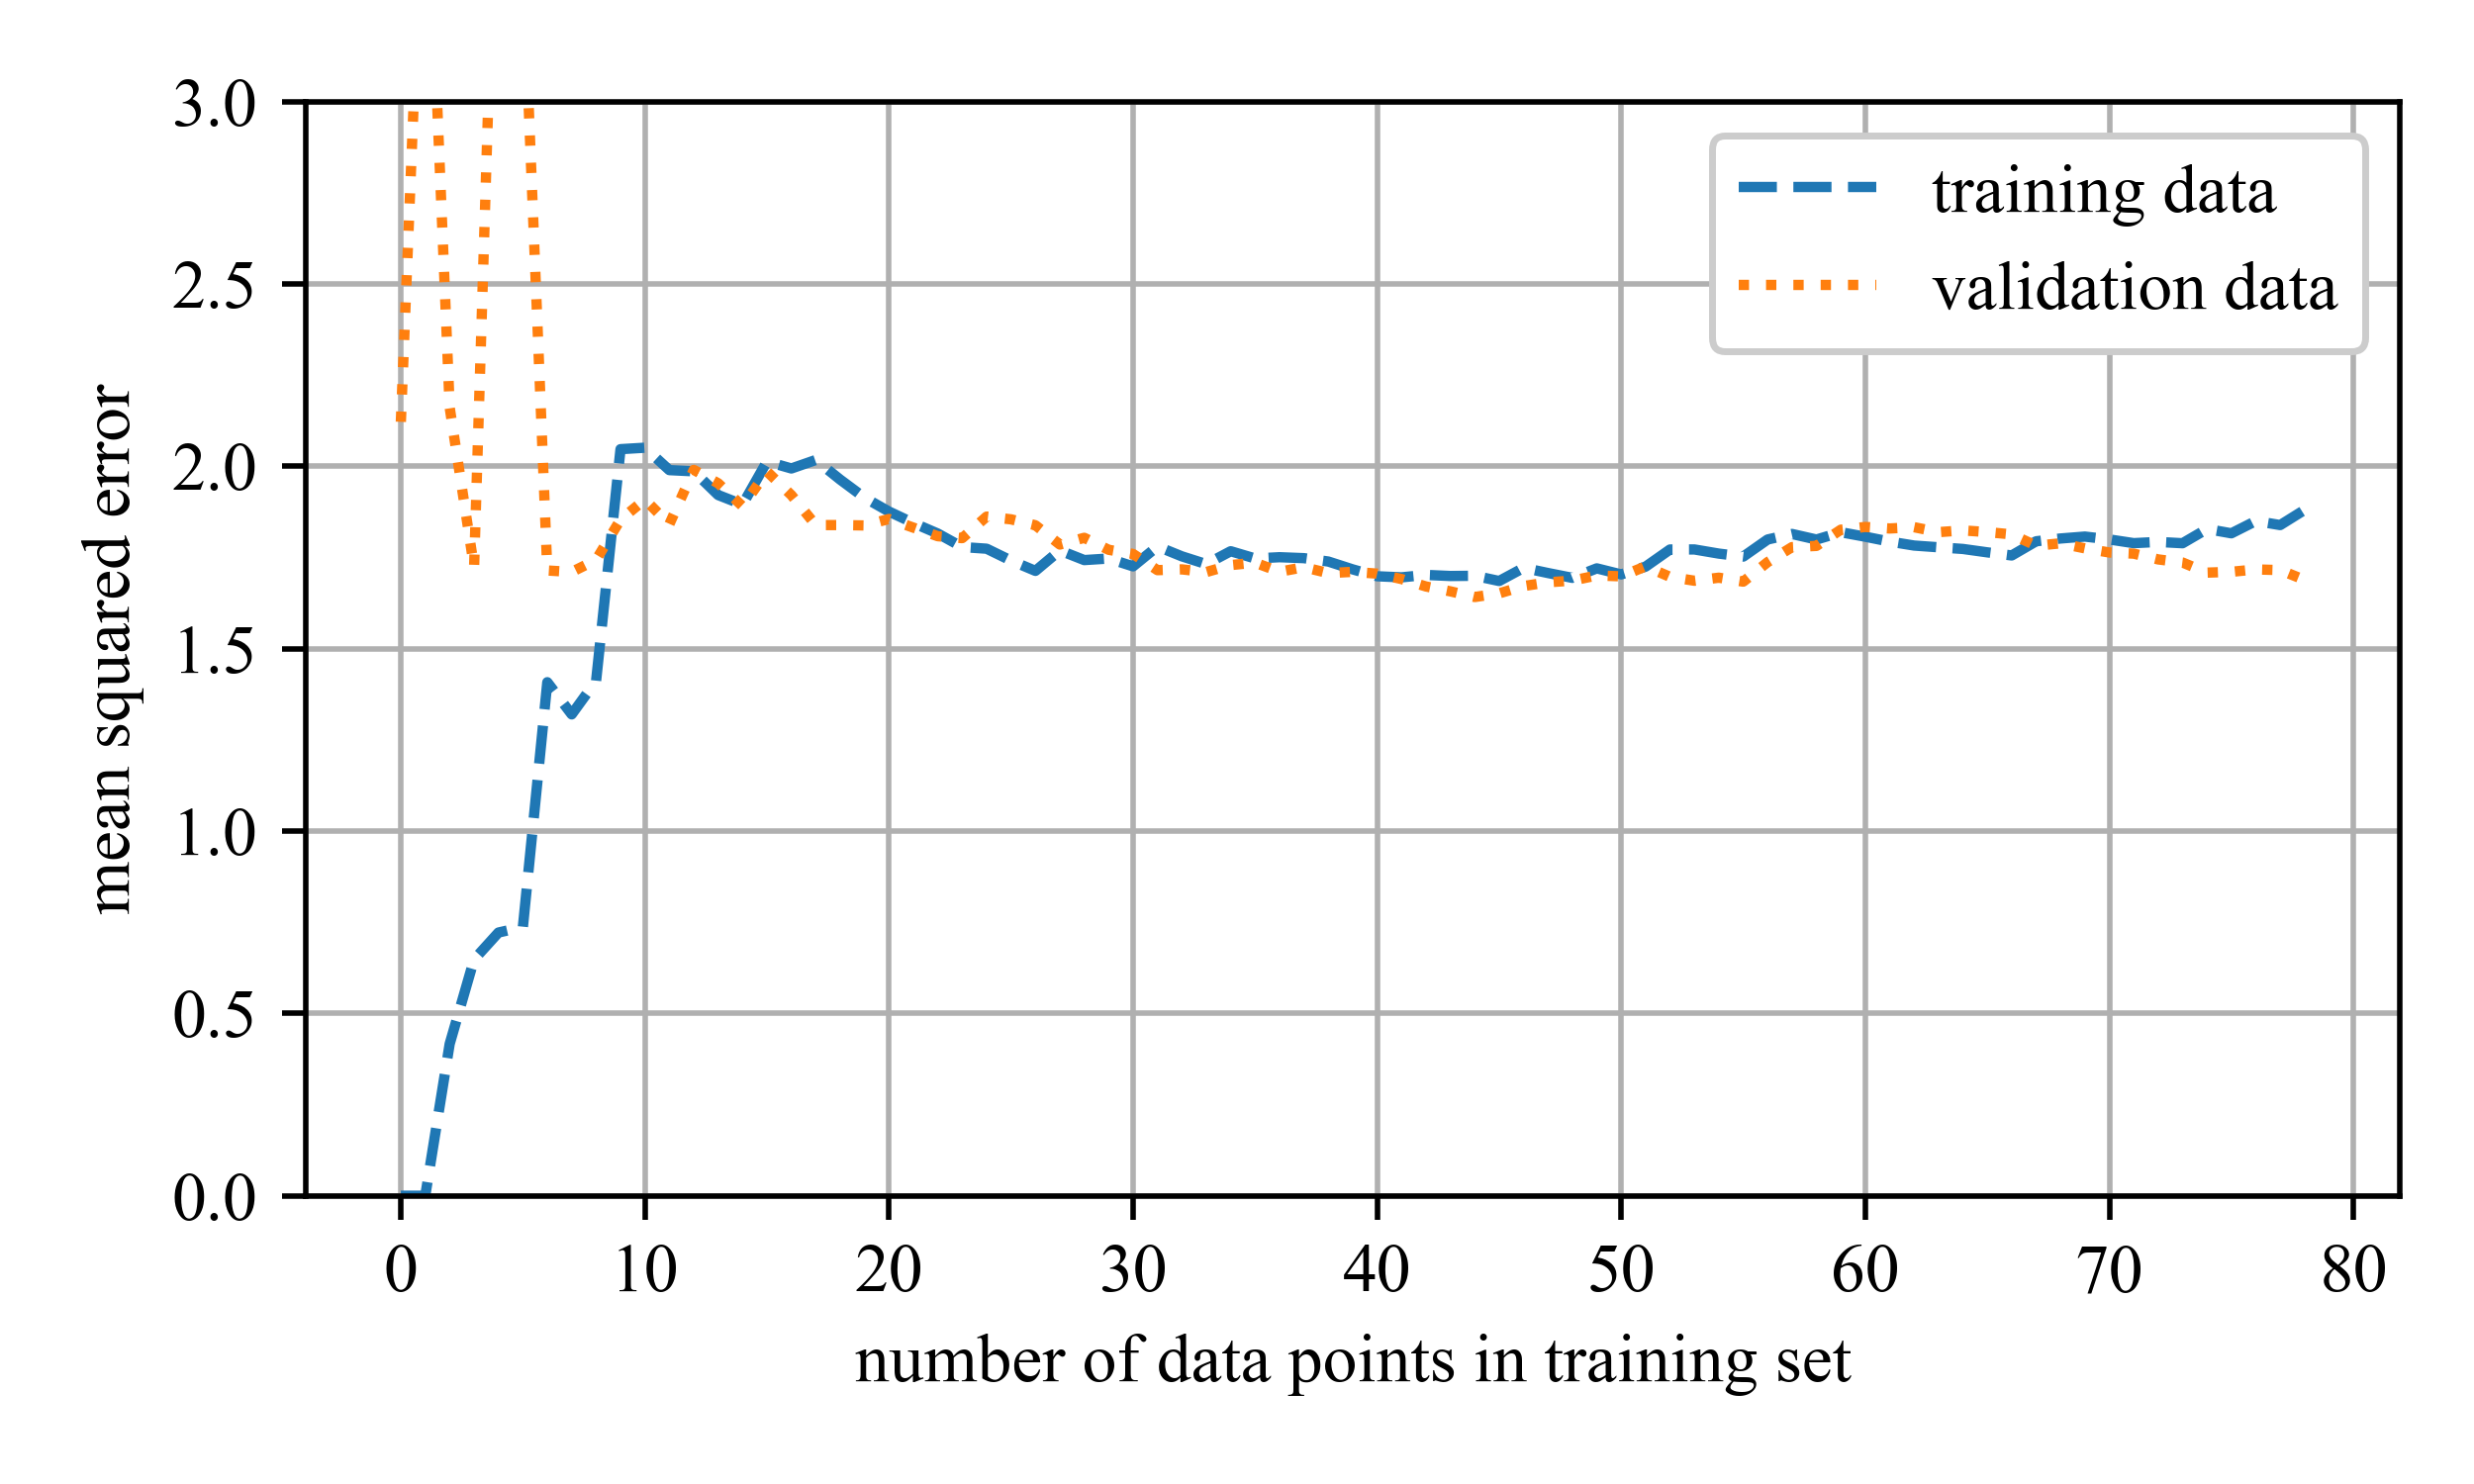
\includegraphics[]{../figures/overfitting_2.png}
\caption{Learning curves for the underfitting linear model (degree=1) where underfitting is evident because both curves have plateaued; they are close together and relatively high.}
\label{fig:overfitting_2}
\end{figure}

Examining the model's behavior in figure~\ref{fig:overfitting_3} on the training set shows a clear trend. With only one or two samples the fit is perfect, so the error curve begins at zero. As additional observations are introduced the model can no longer capture every point exactly, partly because of measurement noise and partly because the underlying relationship is nonlinear, and consequently the training error rises. After a sufficient number of samples the curve flattens out; beyond this plateau adding further data neither markedly lowers nor raises the average error.

\begin{figure}[H]
    \centering
    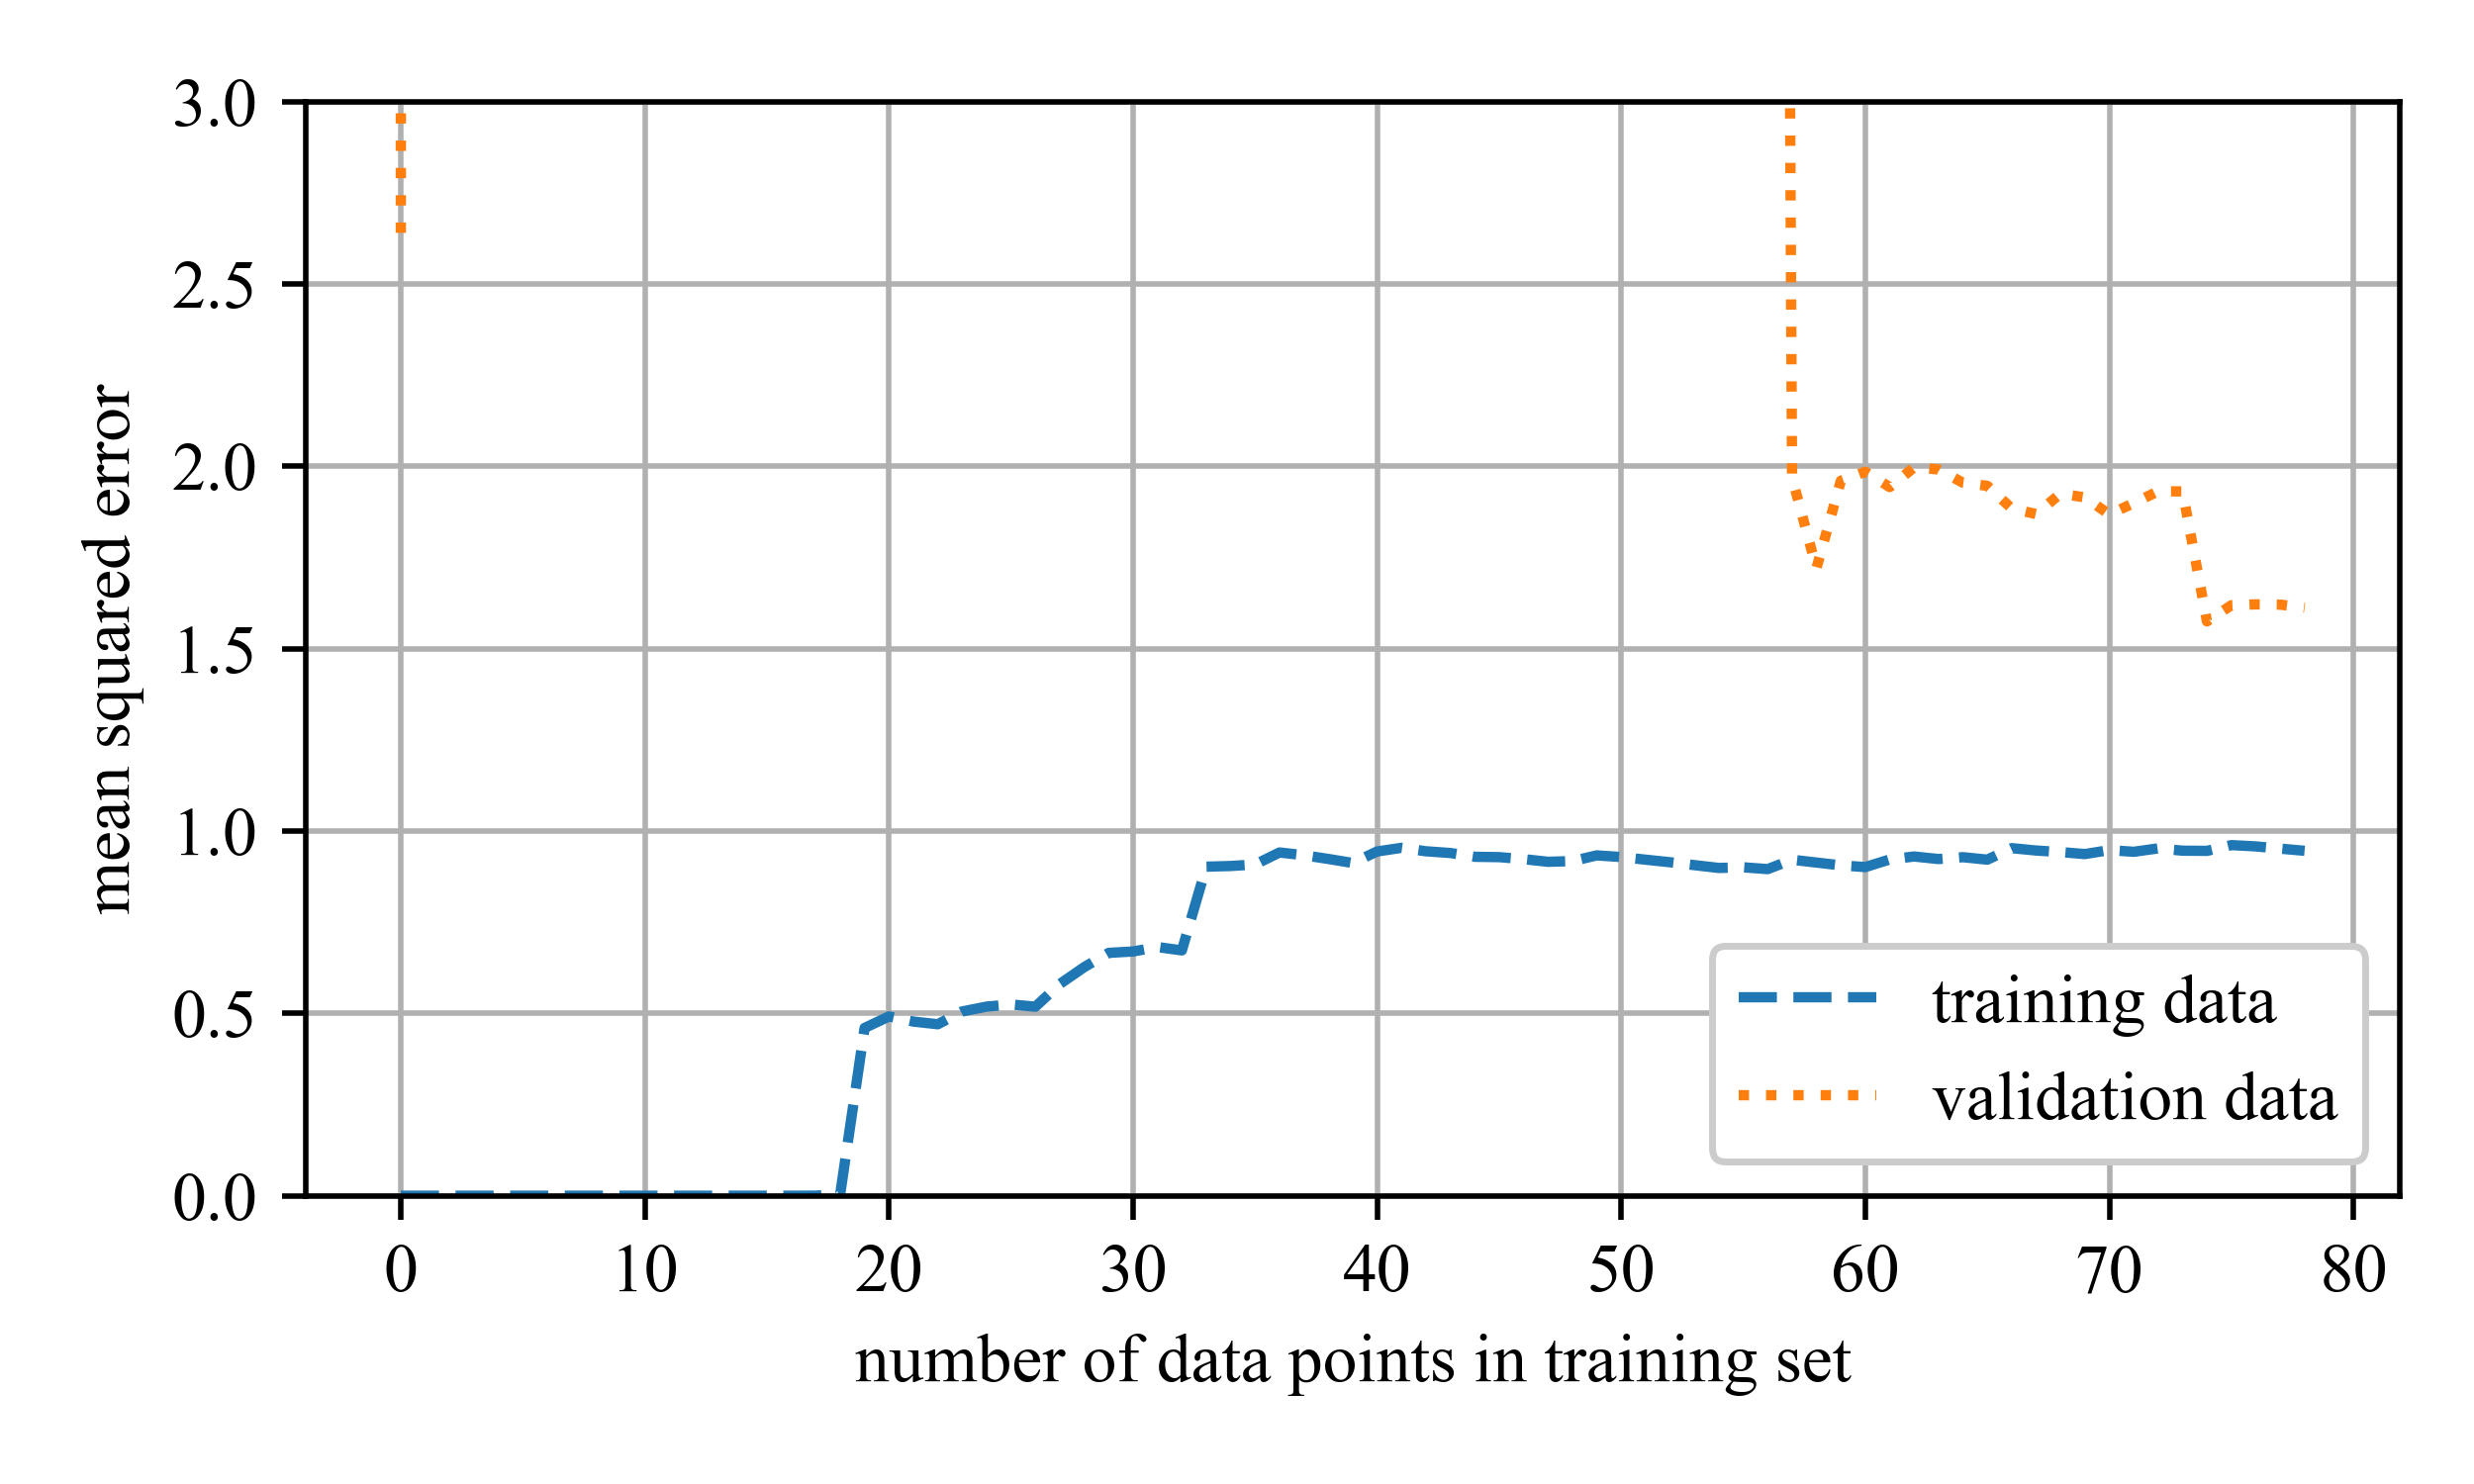
\includegraphics[]{../figures/overfitting_3.png}
    \caption{Learning curves for the overfitting polynomial model (degree=20) showing a significant gap between the curves, which indicates better performance on the training data than on the validation data.}
    \label{fig:overfitting_3}
\end{figure}

Inspection of the validation curve in figure~\ref{fig:overfitting_3}  tells a complementary story. With only a handful of training samples the model cannot generalize, so the validation error starts high. As more examples become available it learns progressively better patterns and the error falls. Eventually, though, the simple linear hypothesis is unable to capture the data's full complexity, causing the decline to flatten out; the validation curve plateaus at nearly the same level as the training curve. Their close proximity and uniformly large values are characteristic of an underfitting model.


Figure~\ref{fig:overfitting_3} displays the learning curves for a model fitted with a 20\textsuperscript{th}-degree polynomial. The overall shape resembles the curves seen earlier, yet two key differences stand out. First, the error on the training set is far lower than that achieved by the Linear Regression model, demonstrating the polynomial's extra flexibility. Second, a pronounced gap separates the training and validation curves, which means the model performs much better on the data it has already seen; this divergence is the hallmark of overfitting. Expanding the training set could reduce the gap, but without additional regularization the risk of overfitting would remain.


Next, let's apply the code using a 2\textsuperscript{nd} order polynomial, which accurately captures the essence of the data without underfitting or overfitting. These results are shown in Figure~\ref{fig:overfitting_4}. Here it can be seen that the training and validation curves again meet after converging, showing a well-fit model.

\begin{figure}[H]
    \centering
    \includegraphics[]{../figures/overfitting_4.png}
    \caption{Learning curves for the optimal polynomial model (degree=2) showing well-aligned curves that plateau at a relatively low error level.}
    \label{fig:overfitting_4}
\end{figure}



\begin{example}
\textbf{Learning Curves}

\noindent This example compares learning curves for linear and polynomial regression models. By plotting training and validation errors as the training set grows, it illustrates how model complexity impacts bias and variance, and helps identify underfitting and overfitting behavior.
\end{example}




\subsection{Regularized Linear Models}
Overfitting is frequently curbed by regularizing the model, meaning you introduce constraints that reduce its effective degrees of freedom and make it harder to memories noise. In a polynomial setting you can achieve this simply by choosing a lower-degree polynomial, while in a linear model you typically add a penalty that discourages large coefficient values. This naturally raises the question: how is regularization expressed mathematically?


\subsubsection{Ridge Regression}

% \todo{Clarify the benefits of ridge regression and refine the description.}



Ridge Regression modifies Linear Regression by adding a regularization term to the cost function, which compels the learning algorithm to fit the data while keeping the model weights as small as possible. The updated cost-function is
\begin{equation}
J(\theta) = \text{MSE}(\theta) + \alpha \frac{1}{2} \sum_{i=1}^{n} \theta_i^2.
\label{eq:ridge_regression}
\end{equation}
The hyperparameter $\alpha$ dictates the degree of regularization. If $\alpha = 0$, Ridge Regression reduces to plain Linear Regression. If $\alpha$ is very high, the model weights are significantly shrunk, resulting in a nearly flat line through the mean of the data. Equation~\ref{eq:ridge_regression} outlines the cost function for Ridge Regression. The bias term $\theta_0$ is not regularized, as indicated by the summation starting from $i = 1$.

\begin{mdframed}[middlelinewidth=0.5mm]
\begin{center}
\bl{NOTE}
\end{center}
The regularization term is only included during the training phase. After training, the model's performance should be evaluated based on the unregularized performance measure.
\end{mdframed}

\begin{figure}[H]
    \centering
    \includegraphics[width=6.5in]{../figures/ridge_regression.png}
    \caption{Visualization of Ridge Regression models with varying $\alpha$ values.}
    \label{fig:ridge_regression}
\end{figure}

Figure~\ref{fig:ridge_regression} illustrates various Ridge models trained on linear data, showcasing different $\alpha$ value. In Figure~\ref{fig:ridge_regression}(a), models are purely Ridge Regression, leading to linear predictions. In Figure~\ref{fig:ridge_regression}(b), the data undergoes Polynomial Regression with Ridge regularization. To do this, the data is first expanded using \texttt{PolynomialFeatures(degree=10)}, then scaled with \texttt{StandardScaler}, and finally, Ridge models are applied to these transformed features.


Increasing $\alpha$ results in flatter (i.e., more reasonable and less extreme) predictions, thereby reducing the model's variance but increasing its bias. Ridge Regression can be performed using a closed-form solution or through Gradient Descent, similar to Linear Regression. The pros and cons for each method mirror those discussed previously. The closed-form solution, an extension of the normal equation, is given by:
\begin{equation}
\hat{\theta} = (X^\text{T} \cdot X + \alpha A)^{-1} \cdot X^\text{T} \cdot y
\end{equation}
where $\alpha$ influences the regularization and $A$ is an $n \times n$ identity matrix with the top-left value replaced by 0 to exclude the bias term. When using Gradient Descent, the derivative of the cost function guides the adjustment toward optimal model parameters.

\begin{example}
\textbf{Ridge Regression}

\noindent This example demonstrates Ridge Regression as a regularized alternative to linear regression. A high-degree polynomial model is fit to noisy data using a pipeline with Ridge regularization, showing how the regularization term reduces overfitting and stabilizes the model.
\end{example}


%\subsubsection{Lasso Regression}
%
%\rd{Discuses other types of regularization.}
%
%
%
%\subsubsection{Elastic Net}
%
%\rd{Discuses other types of regularization.}

\subsection{Early Stopping}

An alternative approach to regularizing iterative learning methods 
(such as Gradient Descent) is to halt training as soon as the validation error hits its lowest point, a strategy known as early stopping. Figure~\ref{fig:early_stopping} illustrates a complex model, specifically a high-degree Polynomial Regression model, being refined through Batch Gradient Descent. Over the course of training, as epochs progress, the model's prediction error (RMSE) on both the training and validation sets decreases. However, after some time, the validation error ceases to decline and begins to increase, signaling that the model is beginning to overfit the training data. By implementing early stopping, training is terminated the moment the validation error reaches its minimum. Geoffrey Hinton praised this method stating, ``Early stopping (is) beautiful free lunch'' due to its simplicity \protect\footnotemark[1].

\footnotetext[1]{Pennington, Jeffrey, Richard Socher, and Christopher D. Manning. ``Glove: Global vectors for word representation.'' Proceedings of the 2014 conference on empirical methods in natural language processing (EMNLP). 2014.}


		\begin{figure}[H]
			\centering
			\includegraphics[width=6in]{../figures/early_stopping.png}
			\caption{An example showing how early stopping can result in a better model as it does not allow for the over-fitting of the training set.}
			\label{fig:early_stopping}
		\end{figure}


\begin{example}
\textbf{Early Stopping}

\noindent This example uses a high-degree polynomial model trained with stochastic gradient descent to demonstrate early stopping. By tracking training and validation errors across epochs, it highlights how halting training early can prevent overfitting and improve generalization.
\end{example}


\pagebreak
\includepdf[pages=1, width= 0.95\textwidth, pagecommand = {\subsection{Examples} \subsubsection*{Example 2.1}\vspace{0.5em}}]{../code/example_2.1_Ames_simple_linear_regression_model.pdf}
\includepdf[pages=2, width= 0.95\textwidth, pagecommand = {\vspace{0.5em}}]{../code/example_2.1_Ames_simple_linear_regression_model.pdf}
\includepdf[pages=3, width= 0.95\textwidth, pagecommand = {\vspace{0.5em}}]{../code/example_2.1_Ames_simple_linear_regression_model.pdf}

\includepdf[pages=1, width= 0.95\textwidth, pagecommand = {\subsubsection*{Example 2.2}\vspace{0.5em}}]{../code/example_2.2_polynominl_regression.pdf}
\includepdf[pages=2, width= 0.95\textwidth, pagecommand = {\vspace{0.5em}}]{../code/example_2.2_polynominl_regression.pdf}

\includepdf[pages=1, width= 0.95\textwidth, pagecommand = {\subsubsection*{Example 2.3}\vspace{0.5em}}]{../code/example_2.3_learning_curves.pdf}
\includepdf[pages=2, width= 0.95\textwidth, pagecommand = {\vspace{0.5em}}]{../code/example_2.3_learning_curves.pdf}

\includepdf[pages=-, width= 0.95\textwidth, pagecommand = {\subsubsection*{Example 2.4}\vspace{0.5em}}]{../code/example_2.4_ridge_regression.pdf}

\includepdf[pages=1, width= 0.95\textwidth, pagecommand = {\subsubsection*{Example 2.5}\vspace{0.5em}}]{../code/example_2.5_early_stopping.pdf}
\includepdf[pages=2, width= 0.95\textwidth, pagecommand = {\vspace{0.5em}}]{../code/example_2.5_early_stopping.pdf}









\end{document}


% Chapter 3 Classification
\documentclass[12pt,letter]{article}
\usepackage{../downey_format}

\begin{document}

	% set the section number, along with figure and equation numbers
	\setcounter{section}{2}	
	\setcounter{figure}{0}   
	\renewcommand\thefigure{\thesection.\arabic{figure}}
	\setcounter{equation}{\thesection}   
	\renewcommand\theequation{\thesection.\arabic{equation}}

	\section{Classification}

In Chapter~1, we examined various tasks that machine learning excels at, such as regression (predicting values) and classification (identifying classes). Having explored linear and polynomial regression in Chapter~2, we now turn our attention to classification in this section.







\subsection{Binary Classifier}

A binary classifier is a model that assigns inputs to one of two distinct classes.
Linear binary classification is a simple but powerful method used to separate data into two distinct classes by drawing a straight decision boundary---such as a line (in 2D) or hyperplane (in higher dimensions)---between them. It works by computing a weighted sum of the input features and applying a threshold to determine the output class. Mathematically, it learns a weight vector $\boldsymbol{\theta}$ and bias term $b$ such that the decision rule can be written as:
\begin{equation}
\hat{y} = \begin{cases}
1 & \text{if } \boldsymbol{\theta}^\text{T} \mathbf{x} + b \geq 0 \\
0 & \text{otherwise}
\end{cases}
\end{equation}
where $\mathbf{x}$ is the input feature vector. During training, the weights are adjusted to minimize classification error, often using gradient descent on a suitable loss functions (e.g., hinge loss or logistic loss). 

Despite its simplicity, the linear classifier is often surprisingly effective, especially when the data is linearly separable or nearly so. An example of such a case is shown in figure~\ref{fig:x_y_plot_linear_classifier} where the three models ($H_1$, $H_2$, and $H_3$) are linear models defined by the hyperparameters $ \boldsymbol{\theta}$ that each correctly classify the data. The challenge then becomes how does one obtain the hyperparameters $ \boldsymbol{\theta}$. To start, we will show that the hyperparameters $ \boldsymbol{\theta}$ can be obtained through gradient descent.



\begin{figure}[H]
    \centering
    \includegraphics[]{../figures/x_y_plot_linear_classifier}
    \caption{Linear classifier that can be implemented with gradient descent.}
    \label{fig:x_y_plot_linear_classifier}
\end{figure}


\begin{data}
\textbf{MNIST (Modified National Institute of Standards and Technology) Dataset}

\noindent  In this chapter, we utilize the MNIST (Modified National Institute of Standards and Technology) dataset, a collection of 70,000 small images of handwritten digits. This dataset is known as ``modified'' because it combines two earlier sets of images: one created by U.S. high school students and another by US Census Bureau employees. First published in 1998, the dataset is particularly suitable for machine learning tasks as each image is labeled with the digit it represents. Each digit has been normalized and centered in a 28x28 pixel frame and anti-aliased to introduce grayscale levels.

Typically, the dataset is split into two parts: the first 60,000 images are used for training, and the remaining 10,000 serve as validation data. It is standard practice to train and test models on the first 60,000 images, reserving the last 10,000 for final validation at the end of the project when the classifier is ready for deployment.

\begin{figure}[H]
    \centering
    \includegraphics[width=6.0in]{../figures/MNIST_data_set}
    \caption{A collection of the 10 digits (0-9) that make up the MNIST data set.}
    \label{fig:MNIST_data_set}
\end{figure}

Scikit-Learn includes a helper function that facilitates the downloading of the MNIST dataset.


\begin{figure}[H]
	\centering
	\includegraphics[width=6.0in]{../figures/MNIST_digit_features}
	\caption{The 784 features that range from 0 to 256 and each represent an 8-bit gray scale pixel for a ``5 digit'' from the MNIST data set.}
	\label{fig:MNIST_digit_features}
\end{figure}


\end{data}


To begin, we simplify our task by focusing on identifying all the ``5''s in the MNIST dataset. This task involves using a binary classifier that checks whether each digit is a 5. The number 5 is notoriously difficult to classify correctly within the MNIST dataset, making it a sensible starting point for binary classification.


\begin{example}
\textbf{MNIST Dataset}

\noindent This example demonstrates how to use \texttt{sklearn.datasets.fetch\_openml} to load the MNIST dataset. It also includes  visualization steps to display sample handwritten digits.
\end{example}



\subsubsection{Regularized Linear Classifier}
%\todo{Consider adding mathematical detail, possibly involving the MSE error cost function.}

A practical algorithm for building this ``5-detector'' is the Regularized Linear Classifier solved with Stochastic Gradient Descent (SGD). The Regularized Linear Classifier offers an efficient and straightforward approach for discriminative learning of linear classifiers under convex loss functions, scaling well with large datasets and maintaining simplicity in implementation as it processes one training example at a time. The main advantages of the Regularized Linear Classifier include:
\begin{itemize}
\item Efficiency.
\item Ease of implementation, providing many opportunities for optimization.
\end{itemize}
However, the Stochastic Gradient Descent classifier also presents certain disadvantages:
\begin{itemize}
\item It requires careful tuning of several hyperparameters, including the regularization parameter and the number of iterations.
\item It is sensitive to feature scaling.
\end{itemize}

\begin{mdframed}[middlelinewidth=0.5mm]
\begin{center}
\bl{NOTE}
\end{center}
The Regularized Linear Classifier solved with Stochastic Gradient Descent is commonly referred to simply called a Stochastic Gradient Descent classifier, despite Stochastic Gradient Descent only being the method used to trail the linear model. This is exemplified by the fact that scikit-learn uses the name \texttt{SGDClassifier} for their model that implements a ``Regularized linear models with stochastic gradient descent (SGD) learning''. 
\end{mdframed}


Given a labeled training set ${(\mathbf x^{(i)},y^{(i)})}_{i=1}^m$ with
$y^{(i)}\in{1,0}$ ($1$ marks the digit ``5''), the regularised linear ``5-detector'' learns a weight vector $\boldsymbol{\theta}$ (bias in the first entry $\boldsymbol{\theta}_1$) by minimising

\begin{equation}
\label{eq:svm_obj}
J(\boldsymbol{\theta}) =
\frac{1}{m}\sum_{i=1}^{m}
\max \bigl(0,1-y^{(i)}\boldsymbol{\theta}^{\text{T}}\mathbf x^{(i)}\bigr)
+ \frac{\lambda}{2}\,\bigl\lVert\boldsymbol{\theta}_{1:}\bigr\rVert_2^{2},
\end{equation}
where the first term is the hinge loss enforcing a unit margin around the decision boundary. The second term applies $\ell_2$-regularisation of strength $\lambda>0$ to all weights except the bias ($\boldsymbol{\theta}_{1}$). Minimising \eqref{eq:svm_obj} with stochastic-gradient descent yields a sparse, margin-maximising classifier that generalises well to unseen handwritten digits.



\begin{example}
\textbf{Regularized Linear Classifier}

\noindent This example trains a regularized linear classifier using \texttt{SGDClassifier} to distinguish the digit ``5'' from other digits in the MNIST dataset. It highlights how regularization helps improve generalization performance by penalizing large weights, and demonstrates basic prediction on a selected digit using a learned linear decision boundary.
\end{example}



\subsection{Performance Measures for Binary Classification}

Assessing the performance of a classifier can be more intricate than evaluating a regressor. Nonetheless, there are numerous performance metrics available that facilitate the comprehensive evaluation of a classifier's effectiveness.



\subsubsection{Confusion Matrix}

First, a brief explanation of Type I and Type II errors. These terms are not exclusive to classification problems in machine learning; they are also crucial in statistical hypothesis testing:

\begin{enumerate}
\item[] \textbf{Type I Error:} False positive (incorrectly rejecting a true null hypothesis)
\item[] \textbf{Type II Error:} False negative (incorrectly failing to reject a false null hypothesis)
\end{enumerate}

These four cases from statistical testing can be combined into a single matrix known as the confusion matrix. In the context of our 5-detector, consider the simplified confusion matrix shown in figure~\ref{fig:confusion_matrix_binary}.

\begin{figure}[H]
    \centering
    \includegraphics[]{../figures/confusion_matrix_binary.png}
    \caption{Confusion matrix binary.}
    \label{fig:confusion_matrix_binary}
\end{figure}


 A effective approach to evaluating classifier performance is to examine the confusion matrix. The essence is to tally the instances where class~A is incorrectly classified as class~B. A well-performing classifier will exhibit high values along the diagonal and lower values elsewhere in the matrix. Each row represents the actual class, while each column represents the predicted class. For instance, to determine how often the classifier misidentified images of 5s as 3s, inspect the intersection of the 5\textsuperscript{th} row and 3\textsuperscript{rd} column in figure~\ref{fig:confusion_matrix}.



\begin{figure}[H]
    \centering
    \includegraphics[width=4in]{../figures/digit_confusion_matrix_limited.png}
    \caption{Confusion matrix for the first 1,000 data points from the MNIST dataset.}
    \label{fig:confusion_matrix}
\end{figure}

\begin{figure}[H]
    \centering
    \includegraphics[]{../figures/confusion_matrix_breakout.png}
    \caption{Confusion matrix breakout.}
    \label{fig:confusion_matrix_breakout}
\end{figure}


Each row in the confusion matrix corresponds to an actual class, while each column corresponds to a predicted class This is diagrammed in figure~\ref{fig:confusion_matrix_breakout}. The first row represents non-5 images (the negative class), and the second row represents images classified as 5s (the positive class). The first column of the first row indicates true negatives (TN), while the second column of the first row shows false positives (FP). The second row denotes images of 5s (the positive class): the first column represents false negatives (FN), and the second column displays true positives (TP). A perfect classifier would only have nonzero values along the main diagonal (from top left to bottom right).






\begin{example}
\textbf{Binary Confusion Matrix}

\noindent This example evaluates a binary classifier trained to detect the digit ``5'' using a confusion matrix. The matrix summarizes the number of true positives, true negatives, false positives, and false negatives. It also visualizes specific misclassifications to help interpret where the model fails, such as incorrectly labeling a ``5'' as not a ``5'' (false negative) or misidentifying another digit as a ``5'' (false positive).
\end{example}



\subsubsection{Accuracy, Precision, and Recall}
The confusion matrix provides detailed information, but sometimes a more concise metric is preferred. Before looking into accuracy, let's define it as
\begin{equation}
\text{Accuracy} = \frac{\text{Number of Correct Predictions}}{\text{Total number of Predictions}}
\end{equation}
or
\begin{equation}
\text{Accuracy} = \frac{TP+TN}{TP+TN+FP+FN}.
\end{equation}
While accuracy offers valuable insights, it's essential to consider the number of falsely classified positive and negative predictions, especially within the context of the problem being addressed. For instance, a 99\% accuracy rate might seem satisfactory for predicting credit card fraud. However, what if a false negative indicates a severe virus or cancer? This is why we need to look deeper into the accuracy formula.


%\todo{Look into replacing the verbage of relevant instances and selected instances with True Positives and True Negatives.}
This is where precision and recall come into play. For this, we will need a definitions of instances
\begin{equation}
\text{Selected instances} = TP + FP
\end{equation}
and
\begin{equation}
\text{Relevant instances} = TP + FN
\end{equation}
which are visualized in figure~\ref{fig:piechart_TP_vs_FP}. With these definitions in mind in mind, let's define precision as
\begin{equation}
\text{Precision} = \frac{\text{selected relevant instances}}{\text{selected instances}},
\end{equation}
or,
\begin{equation}
\text{Precision} = \frac{TP}{TP + FP}.
\end{equation}
One way to achieve perfect precision is to make only one positive prediction and ensure it's correct (precision = 1/1 = 100\%). However, this approach would be impractical as it would ignore most positive instances. Recall complements precision by considering all relevant results, both true positives and false negatives. Recall, also known as sensitivity or true positive rate (TPR), is the ratio of positive instances correctly detected by the classifier. We can define recall as
\begin{equation}
\text{Recall} = \frac{\text{selected relevant instances}}{\text{relevant instances}},
\end{equation}
or,
\begin{equation}
\text{Recall} = \frac{TP}{TP + FN}.
\end{equation}

While the definition of accuracy, precision, and recall may not be immediately intuitive, a visualizations such as that shown in figure~\ref{fig:piechart_TP_vs_FP} can help clarify them.

\begin{figure}[H]
    \centering
    \includegraphics[]{../figures/piechart_TP_vs_FP.png}
    \caption{Visual representation of relevant instances, showing their relation to True Positives (TP) and False Positives (FP). }
    \label{fig:piechart_TP_vs_FP}
\end{figure}


To balance precision and recall, we often use the F1 score, which is the harmonic mean of precision and recall. The F1 score favors classifiers with similar precision and recall, computed as
\begin{equation}
F_1 = 2 \times \frac { \text{precision} \times \text{recall}}{\text{precision} + \text{recall}} = \frac{TP}{TP + \frac{FN + FP}{2}}.
\end{equation}
However, optimizing both precision and recall simultaneously is challenging due to the precision/recall tradeoff. 

Figure~\ref{fig:decision_threshold} illustrates the tradeoffs when adjusting the decision threshold in a Regularized Linear Classifier. By adjusting the classification threshold, we can control the balance between precision and recall. Lowering the threshold increases recall but reduces precision, and vice versa. 
% \todo{add an example on how to adjust the threshold in training.}


\begin{figure}[H]
    \centering
    \includegraphics[]{../figures/decision_threshold.png}
    \caption{Visualization changing thresholds on the classification of digits in a ``5-detector'' and the resulting change in precision and recall.}
    \label{fig:decision_threshold}
\end{figure}

To determine the optimal threshold, it's helpful to plot precision and recall against the threshold values. By default, the classifier in scikit-learn uses a threshold of zero, but this can be adjusted as needed. As illustrated in Figure~\ref{fig:F1_score_plot}, it's relatively straightforward to develop a classifier with nearly any desired precision: simply adjust the threshold to a sufficiently high value. However, it's important to bear in mind that a high-precision classifier may not be very practical if its recall is too low. 




\begin{figure}[H]
    \centering
    \includegraphics[width=6.5in]{../figures/F1_score_plot.png}
    \caption{Visualization of the precision, recall, and F1 score as a function of changing a threshold value. }
    \label{fig:F1_score_plot}
\end{figure}





Figure~\ref{fig:precision_vs_recall} reports a precision vs recall curve that is obtained by changing the threshold of the trained model. At the leftmost part of the precision-recall curve (low recall), precision is highest because the model makes very few positive predictions, and those are likely true positives. As recall increases, the model starts predicting more positives, including more false positives, which reduces precision. The shape of the curve is also important; a steep drop-off indicates that the addition of false positives happens rapidly with increasing recall, whereas a more gradual decline suggests a better balance between precision and recall.

		\begin{figure}[H]
			\centering
			\includegraphics[width=6in]{../figures/precision_recall_curve}
			\caption{The relationship between precision vs recall for a changing threshold value.}
			\label{fig:precision_vs_recall}
		\end{figure}

By analyzing the curve, one can choose a threshold that balances precision and recall according to the specific needs of the application. For instance, in medical diagnosis, high recall is crucial to ensure no cases are missed, even if precision is lower. Additionally, the area under the precision-recall curve (AUC-PR) can be used to compare models. A higher area indicates a model with better performance across all thresholds.

\begin{example}
\textbf{Accuracy, Precision, and Recall}

\noindent This example computes and compares three key classification metrics (accuracy, precision, and recall) for a linear classifier trained to detect the digit ``5'' in the MNIST dataset. It shows both manual and \texttt{sklearn}-based calculations, introduces the F1 score, and visualizes how precision and recall vary with the classification threshold using a precision-recall curve.
\end{example}


\subsection{$k$-fold Cross-validation}
As you've likely observed, training your SGD classifier doesn't always yield consistent results in terms of model performance; hence the ``stochastic'' in stochastic gradient descent. One approach to obtaining a solution closer to the global minimum is to allow the gradient descent algorithm to iterate over more epochs. However, this poses a challenge as it's highly time-consuming and may lead to overfitting the model. Moreover, the variability in model performance makes it difficult to gauge the model's effectiveness.

\begin{figure}[H]
    \centering
    \includegraphics[width=6.5in]{../figures/k-fold_cross-validation_trials}
    \caption{Performance metrics for 500 5-detectors trained either with full data or through $k$-fold cross-validation with 3 folds.}
    \label{fig:k-fold_cross-validation_trials}
\end{figure}

$k$-fold cross-validation offers a more rigorous method for evaluating your algorithm's performance. For instance, consider Figure~\ref{fig:k-fold_cross-validation_trials}, which depicts the performance metrics for 500 classification models trained as 5-detectors. Noticeably, the results obtained using $k$-fold cross-validation exhibit significantly less variability compared to training the classifier on the full dataset. In $k$-fold cross-validation, the training set is divided into smaller subsets for training and validation. The model is trained on these subsets and evaluated on the validation sets. Figure~\ref{fig:grid_search_cross_validation} provides a graphical representation of this technique.

\begin{figure}[H]
    \centering
    \includegraphics[]{../figures/grid_search_cross_validation.png}
    \caption{Illustration of how $k$-fold cross-validation operates.}
    \label{fig:grid_search_cross_validation}
\end{figure}

Of course, Scikit-Learn provides a cross-validation feature, known as \texttt{sk.model\_selection.\allowbreak cross\_val\_score}. This function conducts $k$-fold cross-validation by randomly partitioning the training set into distinct folds. Each fold is used for validation while the rest are used for training the SGD classifier. The reported performance metrics are averaged across all folds. It's important to note that by partitioning the data into folds, the number of samples available for learning is limited, which may result in peculiar classifiers with unusually high or low error rates. Despite being more computationally expensive, this approach effectively utilizes all the data for training and validation.





\begin{example}
\textbf{$k$-fold Cross-Validation}
 
\noindent This example trains a binary classifier to detect the digit ``5'' from the MNIST dataset using Stochastic Gradient Descent (SGD). It first demonstrates how model performance can vary when trained multiple times on the same dataset. Then, by applying $k$-fold cross-validation using \texttt{sk.model\_selection.cross\_val\_predict}, it shows how splitting the data into $k$ subsets helps reduce this variation and provides a more reliable estimate of accuracy, precision, and recall.
\end{example}

\subsection{Multiclass Classification}
Previously, we explored binary classifiers, which distinguish between two classes. Now, we'll explore the use of multiclass classifiers (also known as multinomial classifiers), which can discern between more than two classes. The simplest approach to multiclass classification involves multiple iterations of a binary classifier. There are two primary strategies for achieving this, both of which are considered in the context of the MNIST database challenge:

\begin{itemize}
\item \textbf{One-versus-Rest (OvR)}: This strategy involves creating a system capable of classifying digit images into 10 classes (from 0 to 9) by training 10 binary classifiers, one for each digit (e.g., a 0-detector, a 1-detector, etc.). When classifying an image, the decision score from each classifier is obtained, and the class with the highest score is selected. While sometimes referred to as One-Versus-All (OvA), this term is slightly misleading as it does not involve comparisons against the same class.
\item \textbf{One-versus-one (OvO)}: This approach trains a binary classifier for every pair of digits, such as one for distinguishing between 0s and 1s, another for distinguishing between 0s and 5s, and so forth. If there are $N$ classes, $N \times (N - 1) / 2$ classifiers need to be trained. For the MNIST problem, this translates to training 45 binary classifiers. During classification, the image is evaluated against all 45 classifiers, and the class with the most victories is selected. The primary advantage of OvO is that each classifier only needs to be trained on the relevant portion of the training set for the two classes it distinguishes, which is beneficial for algorithms that scale poorly.
\end{itemize}

\begin{figure}[H]
    \centering
    \includegraphics[width=3.5in]{../figures/one_vs_rest}
    \caption{One-versus-Rest (OvR) classifier for a multi-class dataset.}
    \label{fig:one_vs_rest}
\end{figure}

\begin{figure}[H]
    \centering
    \includegraphics[width=3.5in]{../figures/one_vs_one}
    \caption{One-versus-one (OvO) classifier for a multi-class dataset.}
    \label{fig:one_vs_one}
\end{figure}

Certain algorithms, such as Support Vector Machine classifiers, suffer from scalability issues with larger training sets. Algorithms that do not scale well with large datasets often resort to the OvO approach because training many small classifiers is computationally cheaper than fitting a handful of models on the full data. For most binary classifiers the OvR strategy is the norm. Some methods (including Random Forests and na\"{\i}ve Bayes) support multiclass problems natively and therefore require neither reduction strategy.

\begin{example}
\textbf{Multiclass Regularized Linear Classifier}

\noindent This example extends the use of \texttt{SGDClassifier} to multiclass classification on the MNIST dataset. It compares three approaches: One-vs-Rest (OvR), One-vs-One (OvO), and Scikit-Learn's default automatic strategy. Each method trains multiple binary classifiers to distinguish between the 10 digit classes.
\end{example}



\subsection{Performance Measures for Multiclass Classification}


Assessing a multiclass classifier often poses more challenges compared to evaluating a binary classifier. Nonetheless, many of the principles and methodologies utilized in evaluating binary classifiers can be seamlessly applied to multiclass classifiers as well.


\subsubsection{Confusion Matrix}



%First, you can look at the confusion matrix. You need to make predictions using the \texttt{cross\_val\_predict()} function, then call the \texttt{confusion\_matrix()} function, just like you did earlier:

First, examine the confusion matrix. To do this, generate predictions using the \texttt{cross\_val\_\allowbreak predict()} function, followed by calling the \texttt{confusion\_matrix()} function, similar to your previous steps. The confusion matrix in figure~\ref{fig:digit_confusion_matrix} appears satisfactory, with most images located on the main diagonal, indicating correct classification. However, the 5s appear slightly darker than other digits, suggesting fewer instances of 5s in the dataset or inferior performance of the classifier on 5s. Further investigation confirms both scenarios.




\begin{figure}[H]
    \centering
    \includegraphics[width=4.0in]{../figures/digit_confusion_matrix.png}
    \caption{Confusion matrix for the MNIST data set solved using a one-vs-one classifier with Stochastic Gradient Descent and a $k$-fold of 3.}
    \label{fig:digit_confusion_matrix}
\end{figure}



To turn figure~\ref{fig:digit_confusion_matrix} into a figure that highlights the mistakes, first normalize each entry of the confusion matrix by the number of images in its true class so you compare error rates rather than raw counts that would overweight frequent classes. Then set the diagonal cells to \texttt{NaN} so only the off-diagonal errors remain visible, and plot the resulting matrix. The resulting figure~\ref{fig:digit_confusion_matrix_2} more clearly highlights the errors in the confusion matrix.


\begin{figure}[H]
    \centering
    \includegraphics[width=4.0in]{../figures/digit_confusion_matrix_error.png}
    \caption{Normalized confusion matrix (similar to figure~\ref{fig:digit_confusion_matrix}) with the diagonal removed to emphasize errors.}
    \label{fig:digit_confusion_matrix_2}
\end{figure}

The refined plot facilitates a clear understanding of the classifier's error patterns. Rows represent actual classes, while columns depict predicted classes. Columns corresponding to classes 8 and 9 exhibit brightness, indicating numerous misclassifications as 8s or 9s. Likewise, rows for classes 8 and 9 also appear bright, signifying frequent confusion between 8s, 9s, and other digits. Conversely, some rows, like row 1, display darkness, indicating accurate classification of most 1s (with few exceptions confused with 8s). Notably, errors are asymmetric; for instance, more 5s are misclassified as 8s than vice versa.

Analyzing the confusion matrix provides valuable insights for classifier enhancement. In this case, efforts should concentrate on improving the classification of 8s and 9s, along with addressing the specific 3/5 confusion. Potential strategies include gathering more training data for these digits, devising new features (e.g., counting closed loops), or preprocessing images to emphasize distinguishing patterns (e.g., using Scikit-Image, Pillow, or OpenCV).



\subsubsection{Analyzing Individual Errors}

Analyzing individual errors provides valuable insights into the classifier's behavior and reasons for its failures.

\begin{figure}[H]
    \centering
    \includegraphics[]{../figures/3s_and_5s.png}
    \caption{Confusion matrix showing digits classified as 3s and 5s for the same classifier used to obtain the results shown in figure~\ref{fig:digit_confusion_matrix}.}
    \label{fig:3s_and_5s}
\end{figure}

The left half of figure~\ref{fig:3s_and_5s} contains the blocks for images the classifier labelled as 3, while the right half shows those it labelled as 5. A few misclassified digits are so poorly written that even a human might hesitate, yet many errors look quite clear. Remember that a regularised linear classifier assigns a single weight to every pixel for each class and then sums the weighted pixel intensities to score each class. 

Because just a handful of pixels separate a 3 from a 5, a linear classifier often confuses the two. Their main distinction is the small stroke that joins the top bar to the bottom curve; even a slight shift or rotation of this junction can flip the prediction. The linear model is therefore very sensitive to translations and rotations. Pre-processing the images to center the digits and correct their orientation should lessen the 3-5 confusion and improve performance across the board.
5 

A non-linear model can learn more complex patterns by applying transformations (such as kernel mappings), effectively giving different relative importance to various parts of the image, and would therefore be better equipped to  capture more intricate pixel patterns and more effectively separate these digits.






\begin{example}
\textbf{Multiclass Confusion Matrix}

\noindent This example uses a One-vs-One classifier trained with Stochastic Gradient Descent to evaluate multiclass classification performance on the MNIST dataset. It constructs a confusion matrix using 3-fold cross-validation and visualizes both the raw classification counts and the normalized error rates, helping identify which digits are most commonly misclassified.
\end{example}

\pagebreak
\includepdf[pages=-, width= 0.95\textwidth, pagecommand = {\subsection{Examples} \subsubsection*{Example 3.1}\vspace{0.5em}}]{../code/example_3.1_load_MNIST.pdf}

\includepdf[pages=1, width= 0.95\textwidth, pagecommand = {\subsubsection*{Example 3.2}\vspace{0.5em}}]{../code/example_3.2_MNIST_SGD.pdf}
\includepdf[pages=2, width= 0.95\textwidth, pagecommand = {\vspace{0.5em}}]{../code/example_3.2_MNIST_SGD.pdf}

\includepdf[pages=1, width= 0.95\textwidth, pagecommand = {\subsubsection*{Example 3.3}\vspace{0.5em}}]{../code/example_3.3_confusion_matirx.pdf}
\includepdf[pages=2, width= 0.95\textwidth, pagecommand = {\vspace{0.5em}}]{../code/example_3.3_confusion_matirx.pdf}

\includepdf[pages=1, width= 0.95\textwidth, pagecommand = {\subsubsection*{Example 3.4}\vspace{0.5em}}]{../code/example_3.4_precision_recall_accuracy.pdf}
\includepdf[pages=2, width= 0.95\textwidth, pagecommand = {\vspace{0.5em}}]{../code/example_3.4_precision_recall_accuracy.pdf}

\includepdf[pages=1, width= 0.95\textwidth, pagecommand = {\subsubsection*{Example 3.5}\vspace{0.5em}}]{../code/example_3.5_k-fold_cross-validation.pdf}
\includepdf[pages=2, width= 0.95\textwidth, pagecommand = {\vspace{0.5em}}]{../code/example_3.5_k-fold_cross-validation.pdf}

\includepdf[pages=-, width= 0.95\textwidth, pagecommand = {\subsubsection*{Example 3.6}\vspace{0.5em}}]{../code/example_3.6_Multiclass_SDG.pdf}

\includepdf[pages=-, width= 0.95\textwidth, pagecommand = {\subsubsection*{Example 3.7}\vspace{0.5em}}]{../code/example_3.7_multiclass_confusion_matrix.pdf}

\end{document}



% Chapter 4 Regression-based Classification
\documentclass[12pt,letter]{article}
\usepackage{../downey_format}

\begin{document}

	% set the section number, along with figure and equation numbers
	\setcounter{section}{3}	
	\setcounter{figure}{0}   
	\renewcommand\thefigure{\thesection.\arabic{figure}}
	\setcounter{equation}{0}   
	\renewcommand\theequation{\thesection.\arabic{equation}}

\section{Regression-Based Classification}

Certain algorithms that were first developed for regression can be adapted for classification, and some classifiers can be modified to predict continuous values. Converting a linear regressor into a classifier by adding a logistic link, for instance, retains the original coefficient vector, which makes it easy to see how each input feature influences the decision. As these dual-purpose models expose many of the hyper-parameters found in their regression versions, they often provide more opportunities for fine-tuning and clearer interpretability than algorithms designed purely for classification.

\subsection{Logistic Regression}


Logistic Regression, sometimes called logit regression, models the probability that a sample belongs to a specific class, such as the chance that an email is spam. When this probability exceeds 50\%, the model predicts the positive class (label~``1''); otherwise, it predicts the negative class (label~``0''). It therefore acts as a binary classifier.


The predicted probability is
\begin{equation}
    \hat{p} = h_\theta(X) = \sigma(\theta^\text{T} \cdot X).
\end{equation}
Here $\hat{p}$ is the estimated probability, and $\sigma(\cdot)$ is the sigmoid function, an $S$-shaped curve that maps any real number to the interval $(0,1)$. The logistic function is defined in Equation~\ref{eq:logistic_function} and illustrated in Figure~\ref{fig:sigmoid_function}. As before, $h_\theta(X)$ denotes the hypothesis that the input matrix $X$, augmented with a bias term, belongs to the positive class under the parameters~$\theta$.


\begin{equation}
    \sigma(x) = \frac{1}{1 + e^{-x} }.
    \label{eq:logistic_function}
\end{equation}


		\begin{figure}[H]
			\centering
			\includegraphics[width=6.1in]{../figures/sigmoid_function}
			\caption{Sigmoid function that maps any real-valued input $x$ to a value between 0 and 1. }
			\label{fig:sigmoid_function}
		\end{figure}

Once the probability $\hat{p} = h_\theta(X)$ that an instance $X$ belongs to the positive class has been estimated using Logistic Regression, the prediction ($\hat{y}$) can be made. $\hat{y}$ is calculated as
\begin{equation}
  \hat{y} = 
  \begin{cases}
  0 & \text{if } \hat{p} < 0.5, \\
  1 & \text{if } \hat{p} \ge 0.5.
  \end{cases}
\label{eq:model_prediction}
\end{equation}
Note that $\sigma(x) < 0.5$ when $x < 0$, and $\sigma(x) \ge 0.5$ when $x \ge 0$. Therefore, the Logistic Regression model predicts 0 if $\theta^\text{T} \cdot X$ is negative, and 0 if it is positive.

Now that we understand how logistic regression assigns probabilities and produces predictions, let's walk through a concise example that shows its training procedure and the associated cost function.
Training seeks parameter values $\theta$ that give high predicted probabilities to positive examples ($y = 1$) and low probabilities to negative ones ($y = 0$). This aim is captured by the cost defined in equation~\ref{eq:cost_function}, which evaluates a single training sample $x$. To achieve this, we require a cost function, such as 
\begin{equation}
  C(\theta) = 
  \begin{cases}
  - \log (\hat{p}) & \text{if } y=1, \\
  - \log (1-\hat{p}) & \text{if } y=0.
  \end{cases}
\label{eq:cost_function}
\end{equation}
The considered cost function is plotted in figure~\ref{fig:Logistic_Regression_cost_function}.

\begin{figure}[H]
	\centering
	\includegraphics[width=5.5in]{../figures/Logistic_Regression_cost_function.png}
	\caption{Cost function behavior for classification that heavily penalizes incorrect predictions.}
	\label{fig:Logistic_Regression_cost_function}
\end{figure}

The cost function in equation~\ref{eq:cost_function} behaves intuitively: $-\log(\hat{p})$ increases sharply as $\hat{p} \to 0$, so the loss is large when the model assigns a probability near0 to a positive example. It likewise produces a high loss when the model predicts a probability close to1 for a negative example. Conversely, because $-\log(\hat{p})\to0$ as $\hat{p} \to 1$, the loss becomes negligible when the predicted probability is near1 for a positive instance or near0 for a negative one, aligning with our expectations.



The overall cost, denoted $J(\theta)$, is the mean loss across all $m$ training examples. This metric is commonly called the log-loss and written as 
\begin{equation}
J(\theta) ;=; -\frac{1}{m}\sum_{i=1}^{m}\Big[y^{(i)} \log \bigl(\hat{p}^{(i)}\bigr) ;+; \bigl(1 - y^{(i)}\bigr) \log \bigl(1-\hat{p}^{(i)}\bigr)\Big].
\label{eq:log_loss}
\end{equation}

Because there is no closed-form solution for the parameters $\theta$ (embedded within $\hat{p}$), the minimum must be found with an iterative optimizer. The cost surface is convex, so gradient descent or another suitable algorithm will reach the global minimum provided the learning rate is reasonable and enough iterations are allowed. The gradient of the cost with respect to the $j^\text{th}$ parameter $\theta_j$ is given as
\begin{equation}
\frac{\partial J}{\partial \theta_j} ;=; \frac{1}{m} \sum_{i=1}^{m} \Bigl[\sigma \bigl(\theta^\text{T}X^{(i)}\bigr) - y^{(i)}\Bigr],x^{(i)}_{j}.
\label{eq:Logistic_cost_function_partial_derivatives}
\end{equation}


This equation resembles the partial derivative used in gradient descent. For every training example, it finds the prediction error, multiplies it by the $j^\text{th}$ feature value, and then averages these products over all $m$ samples. With the resulting gradient vector of partial derivatives, you can update the parameters using the Batch Gradient Descent algorithm, completing the training of a Logistic Regression model. Stochastic Gradient Descent performs the update after each single example, while Mini-batch Gradient Descent updates the parameters after processing each mini-batch.



\begin{data}
\textbf{Iris Flower Dataset}

\noindent The Iris dataset, collected by botanist Edgar Anderson in 1935, lists sepal length, sepal width, petal length, and petal width for 150 flowers drawn equally from three species: Iris-Setosa, Iris-Versicolor, and Iris-Virginic  (refer to Figure~\ref{fig:iris_species})a. Statistician Ronald Fisher analysed these measurements in a 1936 study on linear discriminant analysis, and the data have since become a standard benchmark in statistics and machine learning because they are small, clean, and perfectly balanced, making them ideal for testing classification algorithms and visualisation techniques.




\begin{figure}[H]
    \centering
    \includegraphics[width=5.5in]{../figures/iris_species.jpg}
    \caption{Flowers representing three species of iris plants \protect\footnotemark[1]}
    \label{fig:iris_species}
\end{figure}

		\begin{figure}[H]
			\centering
			\includegraphics[width=5.5in]{../figures/Iris_dataset_scatterplot.png}
			\caption{Iris dataset scatterplot showing sepal length vs. sepal width (left) and petal length vs. petal width (right).  }
			\label{Iris_dataset_scatterplot}
		\end{figure}

\footnotetext[1]{Diego Mariano, CC BY-SA 4.0 $<$https://creativecommons.org/licenses/by-sa/4.0$>$, via Wikimedia Commons}
\end{data}



\begin{example}
\textbf{Iris Dataset Exploration}

\noindent This example introduces the Iris dataset (Figure~\ref{fig:iris_species}), originally compiled by Ronald Fisher. It demonstrates how to load the dataset, access feature and label information, and visualize the relationships between sepal and petal measurements across the three iris species.
\end{example}

\subsubsection{1-D Decision Boundaries}

The petal width of Iris-virginica flowers usually lies between 1.4~cm and 2.5~cm, whereas the other two species range from 0.1~cm to 1.8~cm. Because these intervals overlap, the classifier's certainty changes across the scale. Above roughly 2~cm, the model is confident that any given sample is Iris-virginica. Moreover, below 1~cm it is equally sure the flower is not Iris-virginica (This means the model redicts high probability for the class ``Not Iris-Virginica''). In between the limits of the classes, the model is unsure. When you call \texttt{predict()} instead of \texttt{predict\_proba()}, it outputs the most likely class, creating a decision boundary around 1.6~cm where both class probabilities reach 50~percent. Thus, flowers with petal widths greater than 1.6~cm lead to a prediction of Iris-virginica, while flowers with smaller petal widths yield the opposite prediction even if confidence is low.


\begin{figure}[H]
	\centering
	\includegraphics[width=6.2in]{../figures/Iris_dataset_decision_boundary_1D.png}
	\vspace{-3ex}
	\caption{Decision boundary for the flowers of three Iris plant species with C set to $C=10^{10}$ .}
	\label{fig:Iris_dataset_decision_boundary_1D}
\end{figure}

\vspace{-2ex}
\begin{example}
\textbf{1D Logistic Regression}

\noindent This example builds a logistic regression model to classify Iris-Virginica based on a single feature: petal width. It visualizes class probabilities and shows the decision boundary at the 50\% threshold.
\end{example}

	\vspace{-2ex}
\subsubsection{2-D Decision Boundaries}


Figure~\ref{fig:Iris_dataset_decision_boundary_2D} plots petal width against petal length for the Iris samples. After training, the logistic regression model assigns each point the probability that the flower is \textit{Irisvirginica}. The dashed line marks where this probability equals50 \%, forming the decision boundary, which is linear. The parallel contour lines show equal-probability levels from 10\% to 90\%. Points be beyond the top-right line have a greater than 90\% probability  of being classified as Iris-Virginica by the model.



		\begin{figure}[H]
			\centering
			\includegraphics[width=6.2in]{../figures/Iris_dataset_decision_boundary_2D.png}
			\vspace{-3ex}
			\caption{A 2D decision boundary for the Iris dataset.}
			\label{fig:Iris_dataset_decision_boundary_2D}
		\end{figure}

\pagebreak

\begin{example}
\textbf{2D Decision Boundary}

\noindent This example uses logistic regression to classify the Iris-Virginica species based on petal length and width. A 2D decision boundary is visualized in the petal feature space, with prediction regions and probability contours illustrating classifier confidence.
\end{example}



\subsection{Softmax Regression}

Logistic Regression can be generalised to handle many classes in a single model, so there is no need to train and merge several binary classifiers. This multiclass version is called Softmax Regression, or Multinomial Logistic Regression. Softmax Regression provides a straightforward way to perform regression-based classification when more than two classes are present. For an input vector $\mathbf{x}$, the model first computes a score $s_k(\mathbf{x})$ for every class $k$, then turns these scores into class probabilities with the softmax (normalised exponential) function. The score is obtained exactly as in linear regression:
\begin{equation}
s_k(\textbf{x}) = \textbf{x}^\text{T}\pmb{\theta}^{(k)}.
\end{equation}
Here each class has its own parameter vector $\boldsymbol{\theta}^{(k)}$, and the collection of these vectors is usually stored as the rows of a parameter matrix $\Theta$.

After the model has calculated a score for each class given an input $\mathbf{x}$, it converts these scores to probabilities with the softmax function. For class $k$ the predicted probability is
\begin{equation}
\hat{p}_k = \sigma\big(s(\textbf{x}) \big)_k = \frac{\exp \big(s_k(\textbf{x})\big)}{\sum_{j=1}^{K} \exp \big(s_j(\textbf{x}) \big)}.
\label{eq:softmax}
\end{equation}
In this expression, $\mathbf{s}(\mathbf{x})$ is the vector of class scores for the input, $\sigma\bigl(\mathbf{s}(\mathbf{x})\bigr)_k$ is the probability that $\mathbf{x}$ belongs to class $k$, and $K$ is the total number of classes. In short, equation~\ref{eq:softmax} exponentiates each score and then normalises the results by dividing by the sum of all exponentials so the probabilities sum to one.


Like logistic regression, a Softmax~Regression model assigns an input to the class whose predicted probability is largest, which coincides with the class that has the highest score:
\begin{equation}
\hat{y} = \mathop{\text{argmax}}_{k} \sigma \big(\textbf{s}(\textbf{x})\big)_k = \mathop{\text{argmax}}_{k} s_k(\textbf{x}) = \mathop{\text{argmax}}_{k} \big( (\theta^{(k)})^\text{T} \cdot \textbf{x} \big).
\end{equation}


\begin{mdframed}[middlelinewidth=0.5mm]
\begin{center}
\bl{NOTE}
\end{center}
The argmax operator returns the argument that maximises a function. In this setting, it yields the index $k$ for which the estimated probability $\sigma \bigl(s(\mathbf{x})\bigr)_k$ attains its largest value.
\end{mdframed}



With probability estimation and prediction established, we next consider training. The task is to learn parameters that place a large probability on the correct class and correspondingly small probabilities on all others. This objective is met by minimising the cost in equation~\ref{eq:cross_entropy_cost_function}, known as the cross entropy, which heavily penalises the model when it assigns a low probability to the true label. Cross entropy is widely used to measure how well predicted class probabilities agree with the actual classes. The cost function is
\begin{equation}
J(\Theta) = -\frac{1}{m} \sum_{i=1}^{m} \sum_{k=1}^{K} y_k^{(i)} \log (\hat{p}_k^{(i)}).
\label{eq:cross_entropy_cost_function}
\end{equation}

\begin{mdframed}[middlelinewidth=0.5mm]
\begin{center}
\bl{NOTE}
\end{center}
In this expression, $y_k^{(i)} = 1$ when the $i^\text{th}$ sample's true label is class $k$, and $y_k^{(i)} = 0$ otherwise.
\end{mdframed}
When considering only two classes ($K = 2$), it's important to highlight that this cost function aligns with the Logistic Regression's cost function, commonly referred to as log loss (refer to Equation~\ref{eq:log_loss}).

The gradient of the cross-entropy cost with respect to $\boldsymbol{\theta}^{(k)}$ is
\begin{equation}
\nabla_{\theta^{(k)}}J(\Theta) = \frac{1}{m} \sum_{i=1}^{m} (\hat{p}_k^{(i)}-y_k^{(i)} X^{(i)}).
\end{equation}
By computing this vector for each class, you obtain the full gradient, which can then be fed to Gradient~Descent or another optimizer to find the parameter matrix $\Theta$ that minimises the cost.




Applying Softmax Regression to the three-class iris problem in Scikit-Learn is straightforward. The \texttt{LogisticRegression} estimator normally uses one-versus-all when more than two classes are present, but setting \texttt{multi\_class=``multinomial''} activates true Softmax learning. Choose a solver that supports this option, such as \texttt{lbfgs} (see the library documentation). The model applies $\ell_{2}$ regularisation by default, governed by the hyperparameter $C$. After training, a flower with 5~cm long and 2~cm wide petals is classified as Iris-Virginica with probability 94.2\%, while the probability of Iris versicolor is 5.8\%.


\begin{mdframed}[middlelinewidth=0.5mm]
\begin{center}
\bl{NOTE}
\end{center}
The Softmax Regression classifier is multiclass, not multioutput. As such, Softmax Regression can only predict one class at a time, so it works for problems where each input belongs to exactly one category-like classifying an email as spam, promotions, or updates. It can't be used for cases where multiple labels may apply, such as tagging a news article with topics like politics, economics, and technology all at once.
\end{mdframed}


Figure~\ref{fig:Softmax_classification} displays the decision regions, shaded with background colours to mark each class. The borders separating any two classes are straight lines. The plot also includes contour curves for the predicted probability of the Iris-Versicolor class. At the point where all three borders meet, every class receives a probability of 33\%, so the selected class can have a confidence below 50\%.


\begin{figure}[H]
	\centering
	\includegraphics[width=5.5in]{../figures/Softmax_classification.png}
	\caption{Softmax classification for the three iris plant species.}
	\label{fig:Softmax_classification}
\end{figure}



\begin{example}
\textbf{Softmax Classification}

\noindent This example applies softmax regression to classify all three iris species using petal length and width. It builds a multinomial logistic regression model and visualizes the decision boundaries along with confidence contours over the 2D petal feature space.
\end{example}

\pagebreak
\includepdf[pages=-, width= 0.95\textwidth, pagecommand = {\subsection{Examples} \subsubsection*{Example 4.1}\vspace{0.5em}}]{../code/example_4.1_Iris_data_set.pdf}

\includepdf[pages=1, width= 0.95\textwidth, pagecommand = {\subsubsection*{Example 4.2}\vspace{0.5em}}]{../code/example_4.2_Iris_1D_decision_boundary.pdf}
\includepdf[pages=2, width= 0.95\textwidth, pagecommand = {\vspace{0.5em}}]{../code/example_4.2_Iris_1D_decision_boundary.pdf}

\includepdf[pages=1, width= 0.95\textwidth, pagecommand = {\subsubsection*{Example 4.3}\vspace{0.5em}}]{../code/example_4.3_Iris_2D.pdf}
\includepdf[pages=2, width= 0.95\textwidth, pagecommand = {\vspace{0.5em}}]{../code/example_4.3_Iris_2D.pdf}

\includepdf[pages=1, width= 0.95\textwidth, pagecommand = {\subsubsection*{Example 4.4}\vspace{0.5em}}]{../code/example_4.4_softmax.pdf}
\includepdf[pages=2, width= 0.95\textwidth, pagecommand = {\vspace{0.5em}}]{../code/example_4.4_softmax.pdf}


\end{document}




% Chapter 5 Decision Trees
\documentclass[12pt,letter]{article}
\usepackage{../downey_format}




\begin{document}
	
	% set the section number, along with figure and equation numbers
	\setcounter{section}{4}	
	\setcounter{figure}{0}   
	\renewcommand\thefigure{\thesection.\arabic{figure}}
	\setcounter{equation}{0}   
	\renewcommand\theequation{\thesection.\arabic{equation}}
	\section{Decision Trees}


Decision trees are flexible learners that work well for classification, regression, and multi-output problems. A single tree can capture intricate relationships in the data with minimal preprocessing. Each tree also acts as the core building block of ensemble methods such as Random Forests, which are among the most reliable models in modern practice. One limitation is size: a fully grown tree can become quite large, so pruning or depth limits are often applied to control memory use and reduce overfitting.

In this chapter, we will explore the essentials of Decision Trees, starting with their training, visualization, and prediction processes. We will then look into the CART (Classification and Regression Trees) training algorithm, which Scikit-Learn utilizes for constructing Decision Trees. Additionally, we will examine how to regulate the complexity of Decision Trees and adapt them for regression tasks. The chapter concludes by addressing some inherent limitations of Decision Trees. 

\begin{figure}[H]
	\centering
	\includegraphics[width=6.5in]{../figures/decision_tree_basic_concept}
	\caption{The basic connect of a decision tree, showing (a)~how a decision tree is built, and (b)~the developed decision tree.}
	\label{fig:decision_tree_basic_concent}
\end{figure}


\subsection{Decision Tree Classification}


Figure~\ref{fig:decision_tree_boundaries} shows the regions formed by the decision tree. The solid vertical line marks the root split at depth�0, where petal length equals 2.45~cm. All samples on the left of this line belong solely to Iris~setosa, so no further division is needed there. The right half still mixes species, so the depth-1 right child splits again at petal width 1.75~cm, indicated by the dashed line. With \texttt{max\_depth}=2 the tree stops at this point. If \texttt{max\_depth} were increased to�3, the two depth-2 leaves would introduce additional boundaries, drawn as dotted lines.


\begin{figure}[H]
	\centering
	\includegraphics[width=6.5in]{../figures/decision_tree_boundaries}
	\caption{Decision Tree decision boundaries.}
	\label{fig:decision_tree_boundaries}
\end{figure}



A decision tree for the Iris Dataset looks like Figure~\ref{fig:Iris_decision_tree}. Let us examine how the Decision Tree processes predictions. Suppose you come across an iris and need to classify it. Start at the root node (depth=0), which asks whether the flower's petal length is less than 2.45~cm. If the answer is yes, move to the root's left child (depth=1). This child is a leaf, so no further questions follow. The class stored in that leaf is Iris-setosa, and the tree therefore labels the sample as setosa.

\begin{figure}[H]
	\centering
	\includegraphics[width=3.5in]{../figures/Iris_decision_tree}
	\caption{Decision tree for the Iris Dataset trained using the CART algorithms.}
	\label{fig:Iris_decision_tree}
\end{figure}

In Figure~\ref{fig:Iris_decision_tree}, each node reports the split criterion, Gini impurity, sample count, and class distribution. Fill colors denote the predicted species; orange for Setosa, green for Versicolor, and purple for Virginica. Shade intensity conveys confidence: darker hues indicate purer (more certain) leaves, whereas white represents complete uncertainty.
Consider a second iris whose petal length is greater than 2.45~cm. From the root you move to its right child (depth~1). This internal node asks a new question: is the petal width less than 1.75~cm? If yes, the flower is classified as Iris-versicolor (depth=2, left leaf). If no, it is labeled Iris-virginica (depth=2, right leaf). The decision path is clear and easy to follow.

The attributes of a node include:
\begin{itemize}
\item \textit{class}: the class label stored in the leaf.
\item \textit{samples}: the number of training instances that reach the node. For example, $100$ flowers have petal length $>$2.45~cm (depth1, right); among them, $54$ also have petal width $<1.75$~cm (depth2, left).
\item \textit{value}: a three-element vector giving the count of instances from each species at the node. The bottom-right leaf, for instance, contains $0$ Iris-setosa, $1$ Iris-versicolor, and $45$ Iris-virginica.
\item \textit{gini}: the Gini impurity. A node is \emph{pure} when $\textit{gini}=0$, meaning all samples belong to the same class. The depth-1 left node, which holds only Iris-setosa, is pure.
\end{itemize}

The Gini impurity $G_i$ for the $i^{th}$ node is computed using
\begin{equation}
	\label{eq:gini_impurity}
	G_i = 1 - \sum_{k=1}^{n}p_{i,k}^2,
\end{equation}
where $p_{i,k}$ is the proportion of class $k$ instances among the training instances at the $i^{th}$ node. For instance, the Gini score for the depth-2 left node is calculated as follows: $1 - (0/54)^2 - (49/54)^2 - (5/54)^2 \approx 0.168$. We will discuss an alternative impurity measure later.





\subsubsection{Class Probability Estimation}

A Decision Tree can estimate the likelihood that a sample belongs to class~$k$. The algorithm traces the sample's path to its leaf node and then reports the fraction of training instances of class~$k$ found in that leaf. Consider a flower with petals 5cm long and 1.5cm wide. This sample reaches the depth-2 left leaf, which contains 54 training flowers: 0 \textit{Iris}-setosa, 49 \textit{Iris}-versicolor, and 5 \textit{Iris}-virginica. The tree therefore assigns probabilities of 0\%, 90.7\%, and 9.3\% to the three classes, respectively. When asked for a class label, it selects \textit{Iris}-versicolor, the class with the highest probability.

Interestingly, the same estimated probabilities apply throughout the bottom-right rectangle of Figure~\ref{fig:decision_tree_boundaries}, even in a scenario where the petal dimensions are 6~cm by 1.5~cm where one might intuitively expect an Iris-Virginica classification.

\begin{example}
\textbf{Decision Tree Classifier}

\noindent This example uses Scikit-Learn's \texttt{DecisionTreeClassifier} to classify iris species based on petal features. The decision process is visualized using Graphviz, showing the structure of learned rules and how decisions are made based on feature thresholds.  This online viewer is the easiest way to do that \url{https://dreampuf.github.io/GraphvizOnline/}
\end{example}


\subsection{The CART Training Algorithm}

Scikit-Learn trains decision trees with the Classification and Regression Tree (CART) algorithm\footnotemark[1], a process often called ``growing'' the tree. At each node the algorithm splits the local training set into two parts by selecting a feature $k$ and a threshold $t_{k}$, for example ``petal length $\leq 2.45$~cm''. It evaluates every candidate pair $(k,t_{k})$ and chooses the one that yields the purest child nodes, judging purity by a weighted combination of each child's impurity measure and sample count.


\footnotetext[1]{Breiman, Leo. Classification and regression trees. Routledge, 2017}


\begin{figure}[H]
	\centering
	\includegraphics[]{../figures/CART_algorithm}
	\caption{Illustration of the CART algorithm process.}
	\label{fig:algorithm}
\end{figure}


The objective function it aims to minimize during this process is

\begin{equation}
\label{eq:CART_algorithm}
J(k, t_k) = \frac{m_{\text{left}}}{m} G_{\text{left}} + \frac{m_{\text{right}}}{m} G_{\text{right}}. 
\end{equation}

\noindent In this equation, $G_{\text{left}/\text{right}}$ measures the impurity of the left/right subset, and $m_{\text{left}/\text{right}}$ is the number of instances in the left/right subset.
 After the initial split, the algorithm continues to divide the resulting subsets and their subsequent divisions recursively. This recursive process halts when it reaches the predefined maximum depth ({\tt{max\_depth}}) set through a hyperparameter, or if no further impurity-reducing splits can be found.

Unlike linear models that assume a specific data structure, Decision Trees impose few assumptions on their initial data. If not appropriately constrained, a Decision Tree can intricately conform to the training data, leading to overfitting. This model type is described as nonparametric, not due to a lack of parameters, which it can have in abundance, but because the parameters are not predetermined before training, allowing the model's structure to freely mirror the data intricacies. Conversely, a parametric model, like a linear model, has a fixed number of parameters, limiting its flexibility but also minimizing overfitting risks while potentially increasing underfitting risks.

To mitigate overfitting in Decision Trees, it is essential to control the model's freedom during training through regularization. The regularization hyperparameters vary by the algorithm, but typically, the tree's maximum depth can be restricted. In Scikit-Learn, this is managed by the \texttt{max\_depth} hyperparameter, which is unlimited by default. Lowering \texttt{max\_depth} helps regularize the model, thereby reducing overfitting likelihood.

Other parameters in Scikit-Learn's DecisionTreeClassifier also influence the tree's structure:
\begin{itemize}
    \item \texttt{min\_samples\_split}: The minimum number of samples required to split a node.
    \item \texttt{min\_samples\_leaf}: The minimum number of samples a leaf node must have.
    \item \texttt{min\_weight\_fraction\_leaf}: Similar to \texttt{min\_samples\_leaf}, but expressed as a fraction of total weighted instances.
    \item \texttt{max\_leaf\_nodes}: The maximum number of leaf nodes.
    \item \texttt{max\_features}: The maximum number of features evaluated for splitting at each node.
\end{itemize}
Adjusting these parameters by increasing \texttt{min\_}* values or decreasing \texttt{max\_}* values will help regularize the model.

Figure~\ref{fig:decision_tree_regularization} illustrates two Decision Trees trained on the moons dataset: one on the left with default hyperparameters (unrestricted) and another on the right with \texttt{min\_samples\_leaf}=4. The left model appears to be overfitting, whereas the right model, with its restrictions, likely offers better generalization.

\begin{figure}[H]
    \centering
    \includegraphics[width=6.5in]{../figures/decision_tree_regularization}
    \caption{Regularization effects using \texttt{min\_samples\_leaf}}
    \label{fig:decision_tree_regularization}
\end{figure}



\subsubsection{Computational Complexity}

To predict with a Decision Tree the algorithm follows a path from the root to a leaf. Because most trained trees are roughly balanced, this path crosses about
\begin{equation}
T_{\text{predict}} = O \bigl(\log_2 m\bigr),
\label{eq:dt_pred_complexity}
\end{equation}
nodes, where $m$ is the number of training samples. Each node tests a single feature, so the prediction cost in equation~\ref{eq:dt_pred_complexity} is unaffected by the total feature count and is therefore very fast.

Training is costlier. At every split the algorithm scans each candidate feature (or the subset limited by \texttt{max\_features}) over all samples that reach the node. For $n$ input features the total work across all levels is
\begin{equation}
T_{\text{train}} = O \bigl(n \times m \log m\bigr),
\label{eq:dt_train_complexity}
\end{equation}
because the tree has roughly $\log_2 m$ layers and each layer processes a shrinking fraction of the $m$ samples.

When the dataset contains only a few thousand samples, enabling \texttt{presort=True} in Scikit-Learn can shorten training time, but for larger datasets the presorting step turns into a bottleneck and the standard (unsorted) approach is quicker.

\subsubsection{Entropy verse Gini Impurity}

Decision Trees in sklearn use the Gini impurity as the default criterion for node purity, entropy can also be utilized by setting the criterion hyperparameter to ``entropy''. Originally a thermodynamic concept representing molecular disorder, entropy reaches zero when molecules are in a complete state of rest and order. This concept was later adopted in information theory, introduced by Shannon, to quantify the average informational content in messages entropy is zero when all messages are identical. In the realm of Machine Learning, entropy serves as a measure of impurity: it is zero in a dataset if all its elements belong to a single class. The entropy for the i\textsuperscript{th} node is defined as


\begin{equation}
	\label{eq:entropy}
    H_i = - \sum_{\substack{k=1 \\ p_{i,k} \neq 0}}^{n} p_{i,k} \log_{2}(p_{i,k}).
\end{equation}

The choice between Gini impurity and entropy often results in negligible differences, producing similar trees. Gini impurity has a slight computational advantage and is thus the default choice. However, it tends to separate the most frequent class into a distinct branch, whereas entropy generally yields more balanced trees.







\subsection{Decision Tree Regression}

Decision Trees are not limited to classification tasks; they can also be adapted for regression. To illustrate, we use Scikit-Learn's \texttt{DecisionTreeRegressor} to train a regression tree on a noisy linear dataset with \texttt{max\_depth}=2. The structure of this tree is displayed in Figure~\ref{fig:decision_tree_regression}. In contract to the color scheme for classification, the change in color shades here relate to the predicted value of $y$.

\begin{figure}[H]
	\centering
	\includegraphics[width=6.5in]{../figures/decision_tree_regression}
	\caption{A regression model developed using a Decision Tree, showing the: (a) model superimposed over noisy data, and (b) the decision tree developed for the task.}
	\label{fig:decision_tree_regression}
\end{figure}

The workings of a regression tree mirror those of a classification tree, except that each leaf holds a continuous prediction instead of a class label. To obtain a prediction for a sample with $x_1 = 0.6$, trace the path from the root to its leaf; that leaf outputs $0.1106$, which is the average target value among the 110 training instances that reach it. For those instances the mean squared error is $0.0151$.

The predictions from this model are visualized in Figure~\ref{fig:decision_tree_regression_prediction}, with results shown for trees of depth 2 and 3. The deeper tree partitions the input space into more regions, with each region's predicted value being the average target value of the instances it encompasses. The model attempts to organize the regions such that the instances within each are as close as possible to their predicted value.

\begin{figure}[H]
	\centering
	\includegraphics[width=6.5in]{../figures/decision_tree_regression_prediction}
	\caption{Comparison of predictions from two Decision Tree regression models with varying depths.}
	\label{fig:decision_tree_regression_prediction}
\end{figure}

The CART algorithm for regression trees aims to minimize the MSE when splitting the training set, similar to how it minimizes impurity in classification tasks. The cost function minimized by the algorithm is represented as

\begin{equation}
	\label{eq:CART_regression}
    J(k, t_k) = \frac{m_{\text{left}}}{m} \text{MSE}_{\text{left}} + \frac{m_{\text{right}}}{m} \text{MSE}_{\text{right}}.
\end{equation}
Knowing that, 
\begin{equation}
	\text{MSE}_{\text{node}} = \sum\limits_{i \in \text{node}} \left( \hat{y}_{\text{node}} - y^{(i)} \right)^2
\end{equation}
and
\begin{equation}
\hat{y}_{\text{node}} = \frac{1}{m_{\text{node}}} \sum\limits_{i \in \text{node}} y^{(i)}.
\end{equation}

% \quad \text{where} \quad 
%    \left\{
%    \begin{array}{l}
%         \\
%        \hat{y}_{\text{node}} = \frac{1}{m_{\text{node}}} \sum\limits_{i \in \text{node}} y^{(i)}
%    \end{array}
%    \right.
%\end{equation}

Similar to classification, Decision Trees for regression can overfit if not properly regularized. Without regularization, the predictions, as depicted on the left of Figure~\ref{fig:decision_tree_regression_regularized}, can fit the training data excessively. By setting \texttt{min\_samples\_leaf} to 15, a more generalized model is achieved, as shown on the right in the same figure.

\begin{figure}[H]
	\centering
	\includegraphics[width=6.5in]{../figures/decision_tree_regression_regularized}
	\caption{Impact of regularization through setting the minimum number of samples in a leaf on a Decision Tree regression model.}
	\label{fig:decision_tree_regression_regularized}
\end{figure}


\begin{example}
\textbf{Decision Tree Regression}

\noindent This example uses Scikit-Learn's \texttt{DecisionTreeRegressor} to fit a non-linear relationship between input and output data. A tree of depth 4 is trained on noisy linear data and visualized using Graphviz to show how the regression model partitions the input space.
\end{example}



\subsection{Instability}

While Decision Trees offer simplicity, interpretability, versatility, and power, they come with certain drawbacks. A notable limitation is their preference for orthogonal decision boundaries, which makes them highly sensitive to the orientation of the data. For instance, Figure~\ref{fig:decision_tree_training_rotation} illustrates how a simple linearly separable dataset can be perfectly split by a Decision Tree in its original alignment, whereas a 45� rotation results in a convoluted decision boundary. Despite perfect fits to their respective training sets, the rotated tree's model is likely to perform poorly on unseen data. Utilizing Principal Component Analysis (PCA) can often mitigate this issue by reorienting the data more suitably.

\begin{figure}[H]
	\centering
	\includegraphics[width=5.5in]{../figures/decision_tree_training_rotation}
	\caption{Sensitivity to training set rotation. Decision trees create a single clean split on the original data (left), but after a $45^\circ$  rotation they must build a jagged, multi-step boundary; illustrating their sensitivity to feature orientation.}
	\label{fig:decision_tree_training_rotation}
\end{figure}

More broadly, Decision Trees are sensitive to small variations in training data. For instance, changing the seed of the random number generator can lead to a substantially different model, as shown in Figure~\ref{fig:decision_tree_training_details_1}. This variability is partly due to the stochastic nature of the Scikit-Learn's training algorithms; different models may result from the same data unless the \texttt{random\_state} hyperparameter is fixed.

\begin{figure}[H]
	\centering
	\includegraphics[width=6.0in]{../figures/decision_tree_sensitivity}
	\caption{Decision Tree Sensitivity to initial conditions, showing: (a) random number generator seeded with ``1'', and: (b) random number generator seeded with ``2''. \protect\footnotemark[1] }
	\label{fig:decision_tree_training_details_1}
\end{figure}


\footnotetext[1]{``2'' is the author's preferred random number seed.}



\subsection{Random Forest}
\begin{figure}[H]
	\centering
	\includegraphics[width=6.5in]{../figures/random_forest}
	\caption{Random forest with majority voting. \protect\footnotemark[1]} 
	\label{fig:random_forest}
\end{figure}

\footnotetext[1]{TseKiChun, CC BY-SA 4.0 $<$https://creativecommons.org/licenses/by-sa/4.0$>$, via Wikimedia Commons}


Random Forests reduce the high variance of individual decision trees by building many trees on bootstrap samples of the training data and then averaging their outputs. Each tree is grown with a random subset of input features, so the ensemble decorrelates the trees and improves generalisation. For classification problems the forest predicts the class that receives the majority vote, while for regression it returns the mean of the trees' numeric predictions. This bagging strategy limits overfitting and usually yields better performance than a single tree, although it often falls short of the accuracy achieved by gradient-boosted ensembles. Model quality still depends on the data's size, noise level, and feature interactions, and on hyperparameters such as the number of trees, the maximum depth, and the number of features considered at each split.

\pagebreak
\includepdf[pages=1, width= 0.95\textwidth, pagecommand = {\subsection{Examples} \subsubsection*{Example 5.1}\vspace{0.5em}}]{../code/example_5.1_DecisionTree_Classifier.pdf}
\includepdf[pages=2, width= 0.95\textwidth, pagecommand = {\vspace{0.5em}}]{../code/example_5.1_DecisionTree_Classifier.pdf}

\includepdf[pages=-, width= 0.95\textwidth, pagecommand = {\subsubsection*{Example 5.2}\vspace{0.5em}}]{../code/example_5.2_DecisionTree_regression.pdf}



\end{document}



% Chapter 6 Support Vector Machines
\documentclass[12pt,letter]{article}
\usepackage{../downey_format}


\begin{document}
	


	% set the section number, along with figure and equation numbers
	\setcounter{section}{5}	
	\setcounter{figure}{0}   
	\renewcommand\thefigure{\thesection.\arabic{figure}}
	\setcounter{equation}{0}   
	\renewcommand\theequation{\thesection.\arabic{equation}}


	\section{Support Vector Machines}








The core idea of Support Vector Machines becomes clear when viewed geometrically. Figure~\ref{fig:SVM_large_margin_classification} shows a slice of the iris dataset containing two linearly separable species. In the left panel two conventional linear classifiers are drawn; although both label every training point correctly, their separating lines sit very close to several observations, so even a small perturbation could lead to misclassifications on new data. The right panel plots the boundary produced by an SVM. The solid line still splits the classes cleanly, but it is positioned to maximise the distance to the nearest points, leaving the widest possible ``street'' (bounded by the dashed parallels). The samples that lie on these margins are the \emph{support vectors}. This strategy, called large margin classification, usually delivers models that generalise better than those that merely separate the training set.



\begin{figure}[H]
	\centering
	\includegraphics[width=6.5in]{../figures/SVM_large_margin_classification}
	\caption{Large margin classification.}
	\label{fig:SVM_large_margin_classification}
\end{figure}

Observe that the addition of further training instances outside the ``street'' does not influence the decision boundary; it is entirely shaped by the instances situated on the boundary's edge. These pivotal instances are termed support vectors and are highlighted with circles in Figure~\ref{fig:SVM_large_margin_classification}.




\begin{mdframed}[middlelinewidth=0.5mm]
\begin{center}
\bl{NOTE}
\end{center}
The sensitivity of SVMs to feature scales is evident in Figure~\ref{fig:SVM_feature_scaling}. In the left plot, the vertical dimension greatly outweighs the horizontal dimension, resulting in a nearly horizontal ``street.'' However, after applying feature scaling such as using Scikit-Learn's \texttt{StandardScaler} the decision boundary becomes more appropriate, as illustrated in the right plot.

\begin{figure}[H]
	\centering
	\includegraphics[width=6.0in]{../figures/SVM_feature_scaling}
	\caption{Sensitivity of support vectors to feature scaling. }
	\label{fig:SVM_feature_scaling}
\end{figure}

\end{mdframed}




\subsection{Linear SVM Classification}


Hard margin classification demands that all instances be correctly classified without any margin violations. This strict approach faces two significant challenges:
\begin{itemize}
    \item It is only feasible when the data is linearly separable.
    \item It is highly sensitive to outliers.
\end{itemize}
Figure~\ref{fig:SVM_hard_margin} illustrates these challenges using the iris dataset with an added outlier. On the left, achieving a hard margin is impossible due to the outlier. On the right, although a decision boundary is found, it deviates substantially from the optimal boundary shown in Figure~\ref{fig:SVM_large_margin_classification} and is less likely to perform well on new data.


\begin{figure}[H]
	\centering
	\includegraphics[width=6.5in]{../figures/SVM_hard_margin.png}
	\caption{Support vector machines showing (left) an un-separable case, and (right) a separable case with two data points supporting the curbs of the support vector machine. }
	\label{fig:SVM_hard_margin}
\end{figure}


To mitigate the limitations of hard margin classification, a more adaptable model, known as soft margin classification, is often employed. The goal here is to achieve an optimal balance between maximizing the margin width and minimizing margin violations, where instances might fall into the margin or on the incorrect side.

Scikit-Learn's SVM implementations facilitate this balance through the hyperparameter $C$. A smaller value of $C$ results in a wider margin but allows more margin violations, which is beneficial for model flexibility. Conversely, a larger $C$ value tightens the margin, reducing margin violations but at the risk of a less flexible model. Figure~\ref{fig:SVM_hyperparameter_C} demonstrates this trade-off: the left plot with a low $C$ value

\begin{figure}[H]
	\centering
	\includegraphics[width=6.5in]{../figures/SVM_hyperparameter_C.png}
	\caption{SVM margin sizes for different $C$ values.}
	\label{fig:SVM_hyperparameter_C}
\end{figure}


\begin{mdframed}[middlelinewidth=0.5mm]
\begin{center}
\bl{NOTE}
\end{center}
Overfitting in an SVM model can often be addressed by reducing the C value, which increases regularization.
\end{mdframed}


In earlier chapters we placed every model parameter in a single vector $\boldsymbol{\theta}$: the first entry $\theta_0$ acted as the bias, while $\theta_1,\dots,\theta_n$ were the feature weights, and each input was augmented with a constant bias feature $x_0 = 1$. In this chapter we adopt the notation most common for SVMs. The bias is written as $b$, the weight vector as $\mathbf{w}$, and no extra bias feature is appended to the input vectors.

\pagebreak

\subsubsection{Decision Function and Predictions}
A linear SVM classifier determines the class of a new instance $x$ by calculating the decision function
\begin{equation}
\textbf{w}^\text{T} \textbf{x} + b = w_1 x_1 + \cdots + w_n x_n + b.
\end{equation}
If the outcome is positive, the predicted class $\hat{y}$ is the positive class (1); otherwise, it is the negative class (0). This is written as 

\begin{equation}
  \hat{y} = 
  \begin{cases}
  0 & \text{if } \textbf{w}^\text{T} \textbf{x} + b < 0, \\
  1 & \text{if } \textbf{w}^\text{T} \textbf{x} + b \ge 0.
  \end{cases}
\label{eq:Linear_SVM_classifier_prediction}
\end{equation}

Figure~\ref{fig:SVM_decision_function} plots the decision function for a model with two features, so the surface is a plane in $\mathbb{R}^{2}$. The thick solid line marks the decision boundary where the function equals zero. The dashed lines show the loci where the function equals $1$ and $-1$; they run parallel to the boundary and sit at equal distance from it, outlining the margin. Training a linear SVM adjusts $\mathbf{w}$ and $b$ to make this margin as wide as possible while either prohibiting margin violations (hard margin) or keeping them small through a penalty term (soft margin).


\begin{figure}[H]
	\centering
	\includegraphics[]{../figures/SVM_decision_function}
	\caption{Decision function for the Iris Dataset showing how the decision function $h$ cuts through the feature space.}
	\label{fig:SVM_decision_function}
\end{figure}

\pagebreak

\subsubsection{Training Objective}

The slope of the decision function corresponds to the norm of the weight vector, $\|\textbf{w}\|$. Halving this slope causes the decision boundary margins, where the decision function equals $\pm 1$, to double in distance from the decision boundary. Effectively, reducing the norm of $\textbf{w}$ by half doubles the margin. This geometric interpretation is perhaps simpler to visualize in two dimensions, as shown in Figure~\ref{fig:SVM_weight_vectors}. Thus, minimizing $\|\textbf{w}\|$ maximizes the margin.

\begin{figure}[H]
	\centering
	\includegraphics[width=6.5in]{../figures/SVM_weight_vectors}
	\caption{The margin is dependent on the value of the weight vector where a smaller weight vector results in a larger margin and vise versa.}
	\label{fig:SVM_weight_vectors}
\end{figure}

To achieve a large margin while enforcing that no data points fall within the margin (hard margin), we ensure the decision function exceeds +1 for all positive training instances and is less than -1 for all negative instances. Let $t^{(i)}$ equal -1 for negative instances ($y^{(i)} = 0$) and +1 for positive ones ($y^{(i)} = 1$). The constraints then require
\begin{equation}
t^{(i)}(\textbf{w}^\text{T} \textbf{x}^{(i)} + b) \geq 1
\end{equation}
for all training instances. This forms the basis of the hard margin linear SVM classifier optimization problem:

\begin{equation}
\begin{split}
    & \underset{\textbf{w}, b}{\text{minimize}} \;\;\;\; \frac{1}{2}\textbf{w}^\text{T}\textbf{w} \\
    & \text{subject to} \;\;\;\; t^{(i)}(\textbf{w}^\text{T}\textbf{x}^{(i)} + b) \ge 1 \; \text{for} \; i = 1, 2, \ldots, m
\end{split}
\end{equation}


\begin{mdframed}[middlelinewidth=0.5mm]
\begin{center}
\bl{NOTE}
\end{center}
The objective function minimized is $\frac{1}{2}\textbf{w}^\text{T}\textbf{w}$, equivalent to $\frac{1}{2}\|\textbf{w}\|^2$. This formulation is chosen over minimizing $\|\textbf{w}\|$ directly because $\frac{1}{2}\|\textbf{w}\|^2$ offers a straightforward derivative, simply $\textbf{w}$, facilitating gradient calculations. In contrast, $\|\textbf{w}\|$ lacks differentiability at $\textbf{w} = 0$, posing challenges for optimization algorithms, which typically require smooth, differentiable functions to ensure effective optimization.
\end{mdframed}

To formulate the soft margin objective, it is necessary to introduce a slack variable $\zeta^{(i)} \geq 0$ for each instance. This variable, $\zeta^{(i)}$, quantifies the permissible margin violation for the i\textsuperscript{th} instance. Consequently, we face dual objectives: minimizing the slack variables to reduce margin violations and minimizing $\frac{1}{2}\textbf{w}^\text{T}\textbf{w}$ to maximize the margin. The hyperparameter $C$ plays a crucial role here, enabling a balance between these competing objectives. The introduction of $C$ transforms our task into a constrained optimization problem.

\begin{equation}
\begin{split}
    & \underset{\textbf{w}, b, \zeta}{\text{minimize}} \;\;\;\; \frac{1}{2}\textbf{w}^\text{T}\textbf{w} + C \sum_{i=1}^{m} \zeta^{(i)} \\  
    & \text{subject to} \;\;\;\; t^{(i)}(\textbf{w}^\text{T}\textbf{x}^{(i)}+b ) \ge 1 - \zeta^{(i)} \text{ and } \zeta^{(i)} \ge 0 \text{ for } i=1, \; 2, \; \cdots,  \; m 
\end{split}
\end{equation}

\subsubsection{Quadratic Programming}
Both hard margin and soft margin problems are examples of convex quadratic optimization problems with linear constraints, commonly referred to as Quadratic Programming (QP) problems. QP involves solving optimization problems where the objective is a quadratic function and the constraints are linear. This form of programming, established in the 1940s, predates and is distinct from ``computer programming,'' and is sometimes more descriptively termed ``quadratic optimization'' to avoid confusion.

A variety of techniques available through off-the-shelf solvers can address these QP problems, though they extend beyond the scope of this text. The general formulation of a QP problem is as follows:
\begin{equation}
\begin{split}
    & \underset{\textbf{p}}{\text{minimize}} \;\;\;\; \frac{1}{2}\textbf{\textbf{p}}^\text{T}\textbf{H}\textbf{p} + \textbf{f}^\text{T}\textbf{p}\\
    & \text{subject to} \;\;\;\; \textbf{A} \textbf{p} \le \textbf{b}
\end{split}
\label{eq:QP_problem}
\end{equation}
Here, $\textbf{p}$ is an $n_p$-dimensional vector (where $n_p$ is the number of parameters), $\textbf{H}$ is an $n_p \times n_p$ matrix, $\textbf{f}$ is an $n_p$-dimensional vector, $\textbf{A}$ is an $n_c \times n_p$ matrix (with $n_c$ being the number of constraints), and $\textbf{b}$ is an $n_c$-dimensional vector. 

Equation~\ref{eq:QP_problem} defines a standard quadratic program with constraints of the form $\textbf{A} \textbf{p} \le \textbf{b}$. For training a hard margin linear SVM, this setup can be used by choosing parameters that encode the SVM objective and constraints. The solution vector $\textbf{p}$ contains both the bias term and the feature weights. Using this knowledge, a standard QP solver can be applied directly to find the optimal SVM classifier.



\begin{example}
\textbf{Support Vector Machine Classification}

This example applies a linear Support Vector Machine (SVM) classifier to distinguish Iris-Virginica flowers based on petal length and width. The decision boundary is derived after scaling the data, and margins are visualized. Misclassified instances within the margin are identified and marked. The model's performance is assessed using a confusion matrix and F1 score.
\end{example}

\pagebreak
\subsection{Nonlinear SVM Classification}

\begin{figure}[H]
	\centering
	\includegraphics[width=6.5in]{../figures/nonlinear_SVM_example_illustration}
	\caption{Nonlinear SVM example illustration \protect\footnotemark[1]}
	\label{fig:nonlinear_SVM_example_illustration}
\end{figure}
\footnotetext[1]{Machine Learner, CC BY-SA 4.0 $<$https://creativecommons.org/licenses/by-sa/4.0$>$, via Wikimedia Commons}

While linear SVM classifiers are quite effective and perform exceptionally well in various scenarios, many datasets are far from being linearly separable. One strategy to address non-linear datasets is to introduce additional features, such as polynomial feature. Adding features can sometimes transform the dataset into one that is linearly separable. A representation of this technique is shown in \ref{fig:nonlinear_SVM_example_illustration}.

A simple example of converting non-linearly separable variables is shown in figure~\ref{fig:SVM_higher_dimensions} where the left plot displays a simple dataset with a single feature $x_1$. Clearly, this dataset is not linearly separable. However, by adding another feature $x_2 = (x_1)^2$, the dataset becomes perfectly linearly separable in two dimensions.

\begin{figure}[H]
	\centering
	\includegraphics[width=6.5in]{../figures/SVM_higher_dimensions.png}
	\caption{Illustration of SVM in higher dimensions}
	\label{fig:SVM_higher_dimensions}
\end{figure}

You can implement this idea in Scikit-Learn by creating a pipeline that applies a Polynomial Features transformer (introduced in the Regression Chapter), followed by a \texttt{StandardScaler} and a \texttt{LinearSVC}. The approach works nicely on the moons dataset, a toy binary-classification problem in which the samples trace two interleaving half-circles, as illustrated in Figure~\ref{fig:SVM_polynomial_features}. You can generate this dataset with the function \texttt{make\_moons()}.

\begin{figure}[H]
	\centering
	\includegraphics[width=6.5in]{../figures/SVM_polynomial_features.png}
	\caption{Demonstration of a SVM classifier with polynomial features.}
	\label{fig:SVM_polynomial_features}
\end{figure}

\begin{example}
\textbf{Nonlinear Classification}

\noindent This example demonstrates nonlinear classification leveraging \texttt{LinearSVC} in a pipeline with \texttt{preprocessing.PolynomialFeatures} using the \texttt{make\_moons} dataset. A polynomial feature transformation is combined with a linear SVM to classify the data, and the resulting decision boundaries are visualized.
\end{example}


\subsubsection{Kernel trick}

% \todo{Add text on Kernal math if needed}
While adding polynomial features is straightforward and enhances the performance of various Machine Learning algorithms (not limited to SVMs), it presents limitations. Specifically, lower-degree polynomials may not adequately handle complex datasets, and higher-degree polynomials significantly increase the feature count, slowing down the model.

SVMs offer a unique solution through a remarkable mathematical technique known as the kernel trick, which allows for the benefits of high-degree polynomial features without actually expanding the feature space, thereby avoiding a rapid increase in computation. This kernel trick is incorporated within the SVC class. 

In the dual form of an SVM the explicit dot product of two input vectors  
\begin{equation}
\mathbf x^{\mathrm T}\mathbf z
\end{equation} 
is replaced by a kernel function  
\begin{equation}
k(\mathbf x,\mathbf z),
\end{equation}
where $\mathbf x$ and $\mathbf z$ are $n$-dimensional feature vectors representing any two data points in the training set.  
This substitution lets the algorithm construct a linear separator in a (possibly infinite-dimensional) feature space while all calculations still occur in the original input coordinates.


%In the dual form of an SVM the inner product $\mathbf w^\text{T}\mathbf x$ is replaced by a kernel
%\begin{equation}
%k(\mathbf x,\mathbf x),
%\end{equation}
%allowing the algorithm to fit a \textit{linear} separator in a (possibly infinite-dimensional) feature space while the optimisation still takes place in the original coordinates. 

Figure~\ref{fig:SVM_polynomial_kernel} shows configured SVM classifiers using a 3\textsuperscript{rd} and 3\textsuperscript{th} degree polynomial kernel; on the left and right respectively. Adjusting the polynomial degree can help manage model fit: reducing the degree may prevent overfitting, whereas increasing it may be necessary for underfitting scenarios. The `coef0` hyperparameter is crucial as it determines the influence of high versus low-degree polynomials in the model.

\begin{mdframed}[middlelinewidth=0.5mm]
\begin{center}
\bl{NOTE}
\end{center}
A typical method for determining optimal hyperparameter settings involves utilizing grid search techniques. Starting with a broad, coarse grid search to quickly narrow down potential candidates, followed by a more detailed, finer grid search centered on these promising values often yields faster results. Additionally, understanding the function and influence of each hyperparameter aids in efficiently targeting the most relevant areas of the hyperparameter space.
\end{mdframed}


\begin{figure}[H]
	\centering
	\includegraphics[width=6.5in]{../figures/SVM_polynomial_kernel.png}
	\caption{SVM polynomial kernel}
	\label{fig:SVM_polynomial_kernel}
\end{figure}


\subsubsection{Standard Kernels}


Three kernels cover the vast majority of practical cases. 
\begin{itemize}
\item The polynomial kernel captures interactions between input features up to a chosen degree~$d$:
\begin{equation}
k_{\text{poly}}\bigl(\textbf{x},\textbf{z}\bigr)
  = \bigl(\textbf{x}^{\text{T}}\textbf{z} + c\bigr)^{d}
\end{equation}
where $c\!\ge\!0$ is a constant offset.  It is effective when domain knowledge suggests that a low-order combination of variables explains the target.  Keep $d$ modest (typically $d\le5$) and standardise inputs to avoid exploding feature dimensions and overfitting.
\item The radial basis function (RBF) kernel builds smooth, highly flexible decision boundaries:
\begin{equation}
k_{\text{rbf}}\bigl(\textbf{x},\textbf{z}\bigr)
  = \exp\!\bigl(-\gamma \lVert \textbf{x}-\textbf{z}\rVert^{2}\bigr)
\end{equation}
with width parameter $\gamma>0$.  A large $\gamma$ makes the surface too flat (underfitting), while a small $\gamma$ lets every point carve its own pocket (overfitting).  Tune $C$ and $\gamma$ jointly, typically on a logarithmic grid, after x-score standardising the features.
\item The sigmoid kernel adds an S-shaped non-linearity to the inner product:
\begin{equation}
k_{\text{sig}}\bigl(\textbf{x},\textbf{z}\bigr)
  = \tanh\!\bigl(\kappa\,\textbf{x}^{\text{T}}\textbf{z} + \theta\bigr)
\end{equation}
where $\kappa$ controls the slope and $\theta$ the offset.  Although useful for some sparse or text data, this kernel is not always positive-semidefinite, so ensure your software handles the resulting optimisation safely.
\end{itemize}

\begin{example}
\textbf{Polynomial Kernel Trick}

\noindent This example uses the kernel trick to enable an SVM to classify non-linearly separable data using \texttt{SVC} (not \texttt{LinearSVC}). A third-degree polynomial kernel is applied to the moons dataset using Scikit-Learn's \texttt{Pipeline} and \texttt{SVC} tools, producing a curved decision boundary that cleanly separates the classes.
\end{example}


\begin{mdframed}[middlelinewidth=0.5mm]
\begin{center}
\bl{NOTE}
\end{center}
Begin with the RBF kernel as a strong default, explore polynomial kernels when you expect specific interaction orders, and treat the sigmoid option as experimental unless you have evidence it helps.
\end{mdframed}

\subsection{Computational Complexity}

Scikit-Learn provides two main SVM classifiers that trade accuracy for speed in different ways.  
\texttt{LinearSVC} is optimized for large, high-dimensional data when a linear decision boundary is adequate; \texttt{SVC} sacrifices runtime for the expressive power of kernels and thus handles complex, nonlinear patterns. Table \ref{table:SVM_classifiers} highlights how these priorities translate into computational costs and practical constraints and compares them to \texttt{SGDClassifier} for reference.

% Please add the following required packages to your document preamble:
% \usepackage{booktabs}
\begin{table}[H]
\caption{Key characteristics of three Scikit-Learn SVM classifier implementations.}
\label{table:SVM_classifiers}
\begin{tabular}{@{}lllll@{}}
Trule
class & time complexity & out-of-core support & scaling required & kernel trick \\ \midrule
\texttt{LinearSVC} & $O(m \times n)$ & no & yes & no \\
\texttt{SVC} & $O(m^2 \times n)$ to $O(m^3 \times n)$ & no & yes & yes \\
\texttt{SGDClassifier} & $O(m \times n)$ & yes & yes & no \\ \bottomrule
\end{tabular}
\end{table}


\texttt{LinearSVC} builds on the \texttt{liblinear} solver and is limited to \emph{linear} decision boundaries.  
Because it does not apply the kernel trick, its training cost grows almost linearly with both the number of samples~\(m\) and features~\(n\), i.e.\ \(O(m\,n)\). Convergence is controlled by the tolerance parameter \texttt{tol} (denoted \(\epsilon\) in the literature); the default value is usually sufficient, but smaller tolerances can be specified when higher accuracy is critical.

\texttt{SVC}, in contrast, relies on \texttt{libsvm} and \emph{does} support kernel functions. Its computational burden is markedly heavier, between \(O(m^{2} n)\) and \(O(m^{3} n)\) in practice, so training becomes prohibitive once the dataset reaches the hundreds-of-thousands range. Nevertheless, \texttt{SVC} excels on smaller or medium-sized problems that demand nonlinear decision surfaces. Runtime also scales with the average count of non-zero features per instance, meaning sparse high-dimensional inputs remain tractable. 





\vspace{-1ex}
\subsection{SVM Regression}
\label{sec:svr}
\vspace{-1ex}

Support Vector Regression (SVR) adapts the SVM idea to regression by surrounding the prediction curve with a tube of width $\epsilon$; points outside this tube incur a penalty and the optimizer keeps the tube as flat as possible while allowing a limited number of violations governed by the regularization constant $C$.  Conceptually this reverses the classification goal: instead of widening a margin to separate two classes, SVR encourages the data to lie inside the margin, making $\epsilon$ the principal knob that controls how loose the fit may be for both linear and kernel-based models.





\subsubsection{Linear SVR}
\vspace{-1ex}
The presence of additional training instances within the margin does not influence the predictions of the model, rendering it $\epsilon$-insensitive. For linear SVM Regression tasks, the LinearSVR class from Scikit-Learn can be utilized. For instance, 
Figure~\ref{fig:SVM_Regression} demonstrates two linear SVM Regression models trained on random linear data; one features a wide margin ($\epsilon = 1.5$), and the other a narrower margin ($\epsilon = 0.5$).

\begin{figure}[H]
	\centering
	\vspace{-1ex}
	\includegraphics[width=6.5in]{../figures/SVM_Regression.png}
\vspace{-2ex}
	\caption{SVM Regression models with different $\epsilon$ values.}
	\label{fig:SVM_Regression}
\end{figure}

For data that follow an approximately linear trend, the \texttt{LinearSVR} class in Scikit-Learn solves the primal problem directly. It scales in $O(mn)$ time with $m$ samples and $n$ features, making it a practical choice for large data sets where a simple linear fit is adequate.

\subsubsection{Kernel SVR}
\label{sec:svr-kernel}
When the relationship is non-linear, the \texttt{SVR} class employs the kernel trick:
\begin{equation}
f(x)=\sum_{i=1}^{m}(\alpha_i-\alpha_i^{\!*})\,k(x_i,x)+b,
\end{equation}
where $k(\cdot,\cdot)$ is typically RBF or polynomial.  Figure~\ref{fig:SVM_regression_2nd_degree} shows a 2\textsuperscript{nd}-degree polynomial kernel
capturing quadratic structure under various regularisation levels.

The Scikit-lern SVR class, supporting the kernel trick and acting as the regression counterpart to the SVC class, performs well with small to medium-sized datasets but slows considerably as dataset size increases. In contrast, the LinearSVR class, akin to the LinearSVC class, scales linearly with the size of the training set.

\begin{figure}[H]
	\centering
	\includegraphics[width=6.5in]{../figures/SVM_regression_2nd_degree.png}
	\caption{SVM regression with a 2\textsuperscript{nd}-degree polynomial kernel, showcasing different regularization levels.}
	\label{fig:SVM_regression_2nd_degree}
\end{figure}


\begin{example}
\textbf{SVM Polynomial Regression}

This example fits a non-linear regression curve to noisy quadratic data using Support Vector Regression (SVR) with a polynomial kernel. It highlights how SVR models can handle non-linear relationships by introducing a margin of tolerance.
\end{example}

\pagebreak
\includepdf[pages=1, width= 0.95\textwidth, pagecommand = {\subsection{Examples} \subsubsection*{Example 6.1}\vspace{0.5em}}]{../code/example_6.1_Linear_Classification.pdf}
\includepdf[pages=2, width= 0.95\textwidth, pagecommand = {\vspace{0.5em}}]{../code/example_6.1_Linear_Classification.pdf}

\includepdf[pages=1, width= 0.95\textwidth, pagecommand = {\subsubsection*{Example 6.2}\vspace{0.5em}}]{../code/example_6.2_polynomial_features.pdf}


\includepdf[pages=1, width= 0.95\textwidth, pagecommand = {\subsubsection*{Example 6.3}\vspace{0.5em}}]{../code/example_6.3_SVM_Polynomial_kernel.pdf}


\includepdf[pages=1, width= 0.95\textwidth, pagecommand = {\subsubsection*{Example 6.4}\vspace{0.5em}}]{../code/example_6.4_SVM_regression.pdf}









































\end{document}










\pagebreak
\renewcommand{\thepage}{}
\renewcommand\refname{References Cited}
\pagestyle{plain}
\bibliographystyle{Downey_NSF}
\bibliography{Chapter_1_Basic_Concepts}


















\end{document}

